\documentclass[]{tufte-book}

% ams
\usepackage{amssymb,amsmath}

\usepackage{ifxetex,ifluatex}
\usepackage{fixltx2e} % provides \textsubscript
\ifnum 0\ifxetex 1\fi\ifluatex 1\fi=0 % if pdftex
  \usepackage[T1]{fontenc}
  \usepackage[utf8]{inputenc}
\else % if luatex or xelatex
  \makeatletter
  \@ifpackageloaded{fontspec}{}{\usepackage{fontspec}}
  \makeatother
  \defaultfontfeatures{Ligatures=TeX,Scale=MatchLowercase}
  \makeatletter
  \@ifpackageloaded{soul}{
     \renewcommand\allcapsspacing[1]{{\addfontfeature{LetterSpace=15}#1}}
     \renewcommand\smallcapsspacing[1]{{\addfontfeature{LetterSpace=10}#1}}
   }{}
  \makeatother
\fi

% graphix
\usepackage{graphicx}
\setkeys{Gin}{width=\linewidth,totalheight=\textheight,keepaspectratio}

% booktabs
\usepackage{booktabs}

% url
\usepackage{url}

% hyperref
\usepackage{hyperref}

% units.
\usepackage{units}


\setcounter{secnumdepth}{2}

% citations
\usepackage{natbib}
\bibliographystyle{apalike}
%\renewcommand{\bibsection}{\chapter*{References}}

% pandoc syntax highlighting
\usepackage{color}
\usepackage{fancyvrb}
\newcommand{\VerbBar}{|}
\newcommand{\VERB}{\Verb[commandchars=\\\{\}]}
\DefineVerbatimEnvironment{Highlighting}{Verbatim}{commandchars=\\\{\}}
% Add ',fontsize=\small' for more characters per line
\usepackage{framed}
\definecolor{shadecolor}{RGB}{248,248,248}
\newenvironment{Shaded}{\begin{snugshade}}{\end{snugshade}}
\newcommand{\KeywordTok}[1]{\textcolor[rgb]{0.13,0.29,0.53}{\textbf{{#1}}}}
\newcommand{\DataTypeTok}[1]{\textcolor[rgb]{0.13,0.29,0.53}{{#1}}}
\newcommand{\DecValTok}[1]{\textcolor[rgb]{0.00,0.00,0.81}{{#1}}}
\newcommand{\BaseNTok}[1]{\textcolor[rgb]{0.00,0.00,0.81}{{#1}}}
\newcommand{\FloatTok}[1]{\textcolor[rgb]{0.00,0.00,0.81}{{#1}}}
\newcommand{\ConstantTok}[1]{\textcolor[rgb]{0.00,0.00,0.00}{{#1}}}
\newcommand{\CharTok}[1]{\textcolor[rgb]{0.31,0.60,0.02}{{#1}}}
\newcommand{\SpecialCharTok}[1]{\textcolor[rgb]{0.00,0.00,0.00}{{#1}}}
\newcommand{\StringTok}[1]{\textcolor[rgb]{0.31,0.60,0.02}{{#1}}}
\newcommand{\VerbatimStringTok}[1]{\textcolor[rgb]{0.31,0.60,0.02}{{#1}}}
\newcommand{\SpecialStringTok}[1]{\textcolor[rgb]{0.31,0.60,0.02}{{#1}}}
\newcommand{\ImportTok}[1]{{#1}}
\newcommand{\CommentTok}[1]{\textcolor[rgb]{0.56,0.35,0.01}{\textit{{#1}}}}
\newcommand{\DocumentationTok}[1]{\textcolor[rgb]{0.56,0.35,0.01}{\textbf{\textit{{#1}}}}}
\newcommand{\AnnotationTok}[1]{\textcolor[rgb]{0.56,0.35,0.01}{\textbf{\textit{{#1}}}}}
\newcommand{\CommentVarTok}[1]{\textcolor[rgb]{0.56,0.35,0.01}{\textbf{\textit{{#1}}}}}
\newcommand{\OtherTok}[1]{\textcolor[rgb]{0.56,0.35,0.01}{{#1}}}
\newcommand{\FunctionTok}[1]{\textcolor[rgb]{0.00,0.00,0.00}{{#1}}}
\newcommand{\VariableTok}[1]{\textcolor[rgb]{0.00,0.00,0.00}{{#1}}}
\newcommand{\ControlFlowTok}[1]{\textcolor[rgb]{0.13,0.29,0.53}{\textbf{{#1}}}}
\newcommand{\OperatorTok}[1]{\textcolor[rgb]{0.81,0.36,0.00}{\textbf{{#1}}}}
\newcommand{\BuiltInTok}[1]{{#1}}
\newcommand{\ExtensionTok}[1]{{#1}}
\newcommand{\PreprocessorTok}[1]{\textcolor[rgb]{0.56,0.35,0.01}{\textit{{#1}}}}
\newcommand{\AttributeTok}[1]{\textcolor[rgb]{0.77,0.63,0.00}{{#1}}}
\newcommand{\RegionMarkerTok}[1]{{#1}}
\newcommand{\InformationTok}[1]{\textcolor[rgb]{0.56,0.35,0.01}{\textbf{\textit{{#1}}}}}
\newcommand{\WarningTok}[1]{\textcolor[rgb]{0.56,0.35,0.01}{\textbf{\textit{{#1}}}}}
\newcommand{\AlertTok}[1]{\textcolor[rgb]{0.94,0.16,0.16}{{#1}}}
\newcommand{\ErrorTok}[1]{\textcolor[rgb]{0.64,0.00,0.00}{\textbf{{#1}}}}
\newcommand{\NormalTok}[1]{{#1}}

% longtable
\usepackage{longtable,booktabs}

% multiplecol
\usepackage{multicol}

% strikeout
\usepackage[normalem]{ulem}

% morefloats
\usepackage{morefloats}

% force floats added by CII
\usepackage{float}
\floatplacement{figure}{H}

\let\oldrule=\rule 
\renewcommand{\rule}[1]{\oldrule{\linewidth}}


% tightlist macro required by pandoc >= 1.14
\providecommand{\tightlist}{%
  \setlength{\itemsep}{0pt}\setlength{\parskip}{0pt}}

% title / author / date
\title{ModernDive}

\author{Chester Ismay and Albert Y. Kim}
\date{2017-01-09}

\usepackage{booktabs}
\usepackage{longtable}
\usepackage{framed,color}
\definecolor{shadecolor}{RGB}{248,248,248}
\usepackage{float}

\ifxetex
  \usepackage{letltxmacro}
  \setlength{\XeTeXLinkMargin}{1pt}
  \LetLtxMacro\SavedIncludeGraphics\includegraphics
  \def\includegraphics#1#{% #1 catches optional stuff (star/opt. arg.)
    \IncludeGraphicsAux{#1}%
  }%
  \newcommand*{\IncludeGraphicsAux}[2]{%
    \XeTeXLinkBox{%
      \SavedIncludeGraphics#1{#2}%
    }%
  }%
\fi

%% Need to clean up
\newenvironment{rmdblock}[1]
  {\begin{shaded*}
  \begin{itemize}
  \renewcommand{\labelitemi}{
    \raisebox{-.7\height}[0pt][0pt]{
  %    {\setkeys{Gin}{width=3em,keepaspectratio}\includegraphics{images/#1}}
    }
  }
  \item
  }
  {
  \end{itemize}
  \end{shaded*}
  }
%% Probably can be omitted
\newenvironment{rmdnote}
  {\begin{rmdblock}{note}}
  {\end{rmdblock}}
\newenvironment{rmdcaution}
  {\begin{rmdblock}{caution}}
  {\end{rmdblock}}
\newenvironment{rmdimportant}
  {\begin{rmdblock}{important}}
  {\end{rmdblock}}
\newenvironment{rmdtip}
  {\begin{rmdblock}{tip}}
  {\end{rmdblock}}
\newenvironment{rmdwarning}
  {\begin{rmdblock}{warning}}
  {\end{rmdblock}}
\newenvironment{learncheck}
  {\begin{rmdblock}{warning}}
  {\end{rmdblock}}
\newenvironment{review}
  {\begin{rmdblock}{warning}}
  {\end{rmdblock}}

% To tweak tufte layout
\geometry{
  left=0.8in, % left margin
  textwidth=35pc, % main text block
  marginparsep=1pc, % gutter between main text block and margin notes
  marginparwidth=8pc % width of margin notes
}

\begin{document}

\let\allcaps=\relax
\maketitle



{
\setcounter{tocdepth}{1}
\tableofcontents
}

\chapter{Preamble}\label{preamble}

\section{Principles of this Book - For
Instructors}\label{principles-of-this-book---for-instructors}

These are some principles we keep in mind. If you agree with them, this
might be the book for you.

\begin{enumerate}
\def\labelenumi{\arabic{enumi}.}
\tightlist
\item
  \textbf{Blur the lines between lecture and lab}

  \begin{itemize}
  \tightlist
  \item
    Laptops and open source software are rendering the lab/lecture
    dichotomy ever more archaic.
  \item
    It's much harder for students to understand the importance of using
    the software if they only use it once a week or less. They forget
    the syntax in much the same way someone learning a foreign language
    forgets the rules.
  \end{itemize}
\item
  \textbf{Focus on the entire data/science research pipeline}

  \begin{itemize}
  \tightlist
  \item
    Grolemund and Wickham's
    \href{http://r4ds.had.co.nz/introduction.html}{graphic}
  \item
    George Cobb argued for
    \href{https://arxiv.org/abs/1507.05346}{``Minimizing prerequisites
    to research''}
  \end{itemize}
\item
  \textbf{It's all about data, data, data}

  \begin{itemize}
  \tightlist
  \item
    We leverage R packages for rich/complex, yet easy-to-load data sets.
  \item
    We've heard it before: ``You can't teach \texttt{ggplot2} for data
    visualization in intro stats!'' We, like
    \href{http://varianceexplained.org/r/teach_ggplot2_to_beginners/}{David
    Robinson}, are more optimistic and we've had success doing so.
  \item
    \texttt{dplyr} is a
    \href{http://chance.amstat.org/2015/04/setting-the-stage/}{game
    changer} for data manipulation: the verb describing your desired
    data action \emph{is} the command name!
  \end{itemize}
\item
  \textbf{Use simulation/resampling for intro stats, not
  probability/large sample approximation}

  \begin{itemize}
  \tightlist
  \item
    Reinforce concepts, not equations, formulas, and probability tables.
  \item
    To this end, we're big fans of the
    \href{https://github.com/ProjectMOSAIC/mosaic}{\texttt{mosaic}}
    package's \texttt{shuffle()}, \texttt{resample()}, and \texttt{do()}
    functions for sampling and simulation.
  \end{itemize}
\item
  \textbf{Don't fence off students from the computation pool, throw them
  in!}

  \begin{itemize}
  \tightlist
  \item
    Don't teach them coding/programming per se, but computational and
    algorithmic thinking.
  \item
    Drawing Venn diagrams delineating statistics, computer science, and
    data science is also ever more archaic; embrace computation!
  \end{itemize}
\item
  \textbf{Complete reproducibility}

  \begin{itemize}
  \tightlist
  \item
    We find it frustrating when textbooks give examples but not the
    source code and the data itself. We not only give you the source
    code for all examples, but also the source code for the whole book!
  \item
    We encourage use of R Markdown to foster notions of reproducible
    research.
  \item
    \textbf{Ultimately the best textbook is one you've written yourself}

    \begin{itemize}
    \tightlist
    \item
      You best know your audience, their background, and their
      priorities and you know best your own style and the types of
      examples and problems you like best. Customizability is the
      ultimate end.
    \item
      A new paradigm for textbooks? Versions, not editions? Pull
      requests, crowd-sourcing, and development versions?
    \end{itemize}
  \end{itemize}
\end{enumerate}

\section{Contribute}\label{contribute}

\begin{itemize}
\tightlist
\item
  This book is in beta testing and is currently at Version 0.1.0.9000.
  If you would like to receive periodic updates on this book and other
  similar projects, please fill out this
  \href{https://goo.gl/forms/IxiwBeEnk72NxMMx2}{Google Form}.
\item
  The source code for this book is available for download/forking on
  \href{https://github.com/ismayc/moderndiver-book}{GitHub}. If you
  click on the \textbf{release} link near the top of the page there, you
  can download all of the source code for whichever release version
  you'd like to work with and use. If you find typos or other errors or
  have suggestions on how to better word something in the book, please
  create a pull request too! We also welcome issue creation. Let's all
  work together to make this book as great as possible for as many
  students and instructors as possible.
\item
  Please feel free to modify the book as you wish for your own needs!
  All we ask is that you list the authors field above as ``Chester
  Ismay, Albert Y. Kim, and YOU!''
\item
  We'd also appreciate if you let us know what changes you've made and
  how you've used the textbook. We'd love some data on what's working
  well and what's not working so well.
\end{itemize}

\section{Getting Started - For
Students}\label{getting-started---for-students}

This book was written using the \textbf{bookdown} R package from Yihui
Xie \citep{R-bookdown}. In order to follow along and run the code in
this book on your own, you'll need to have access to R and RStudio. You
can find more information on both of these with a simple Google search
for ``R'' and for ``RStudio.'' An introduction to using R, RStudio, and
R Markdown is also available in a free book
\href{http://ismayc.github.io/rbasics-book}{here} \citep{usedtor2016}.
It is recommended that you refer back to this book frequently as it has
GIF screen recordings that you can follow along with as you learn.

We will keep a running list of R packages you will need to have
installed to complete the analysis as well here in the
\texttt{needed\_pkgs} character vector. You can check if you have all of
the needed packages installed by running all of the lines below in the
next chunk of R code. The last lines including the \texttt{if} will
install them as needed (i.e., download their needed files from the
internet to your hard drive and install them for your use).

You can run the \texttt{library} function on them to load them into your
current analysis. Prior to each analysis where a package is needed, you
will see the corresponding \texttt{library} function in the text. Make
sure to check the top of the chapter to see if a package was loaded
there.

\begin{Shaded}
\begin{Highlighting}[]
\NormalTok{needed_pkgs <-}\StringTok{ }\KeywordTok{c}\NormalTok{(}\StringTok{"nycflights13"}\NormalTok{, }\StringTok{"dplyr"}\NormalTok{, }\StringTok{"ggplot2"}\NormalTok{, }\StringTok{"knitr"}\NormalTok{, }
  \StringTok{"okcupiddata"}\NormalTok{, }\StringTok{"dygraphs"}\NormalTok{, }\StringTok{"rmarkdown"}\NormalTok{, }\StringTok{"mosaic"}\NormalTok{, }\StringTok{"ggplot2movies"}\NormalTok{)}

\NormalTok{new.pkgs <-}\StringTok{ }\NormalTok{needed_pkgs[!(needed_pkgs %in%}\StringTok{ }\KeywordTok{installed.packages}\NormalTok{())]}

\NormalTok{if(}\KeywordTok{length}\NormalTok{(new.pkgs)) \{}
  \KeywordTok{install.packages}\NormalTok{(new.pkgs, }\DataTypeTok{repos =} \StringTok{"http://cran.rstudio.com"}\NormalTok{)}
\NormalTok{\}}
\end{Highlighting}
\end{Shaded}

\section*{Colophon}\label{colophon}
\addcontentsline{toc}{section}{Colophon}

The source of the book is available
\href{https://github.com/ismayc/moderndiver-book}{here} and was built
with versions of R packages (and their dependent packages) given below.
This may not be of importance for initial readers of this book, but the
hope is you can reproduce a duplicate of this book by installing these
versions of the packages.

\begin{longtable}{lllll}
\toprule
package & * & version & date & source\\
\midrule
assertthat &  & 0.1 & 2013-12-06 & CRAN (R 3.3.0)\\
backports &  & 1.0.4 & 2016-10-24 & CRAN (R 3.3.0)\\
base64enc &  & 0.1-3 & 2015-07-28 & CRAN (R 3.3.0)\\
BH &  & 1.62.0-1 & 2016-11-19 & CRAN (R 3.3.2)\\
bitops &  & 1.0-6 & 2013-08-17 & CRAN (R 3.3.0)\\
\addlinespace
caTools &  & 1.17.1 & 2014-09-10 & CRAN (R 3.3.0)\\
colorspace &  & 1.3-2 & 2016-12-14 & CRAN (R 3.3.2)\\
curl &  & 2.3 & 2016-11-24 & CRAN (R 3.3.2)\\
DBI &  & 0.5-1 & 2016-09-10 & CRAN (R 3.3.0)\\
dichromat &  & 2.0-0 & 2013-01-24 & CRAN (R 3.3.0)\\
\addlinespace
digest &  & 0.6.11 & 2017-01-03 & CRAN (R 3.3.2)\\
dplyr &  & 0.5.0 & 2016-06-24 & CRAN (R 3.3.0)\\
dygraphs &  & 1.1.1.4 & 2017-01-04 & CRAN (R 3.3.2)\\
evaluate &  & 0.10 & 2016-10-11 & CRAN (R 3.3.0)\\
ggdendro &  & 0.1-20 & 2016-04-27 & CRAN (R 3.3.0)\\
\addlinespace
ggplot2 &  & 2.2.1 & 2016-12-30 & CRAN (R 3.3.2)\\
ggplot2movies &  & 0.0.1 & 2015-08-25 & CRAN (R 3.3.0)\\
gridExtra &  & 2.2.1 & 2016-02-29 & CRAN (R 3.3.0)\\
gtable &  & 0.2.0 & 2016-02-26 & CRAN (R 3.3.0)\\
highr &  & 0.6 & 2016-05-09 & CRAN (R 3.3.0)\\
\addlinespace
hms &  & 0.3 & 2016-11-22 & CRAN (R 3.3.2)\\
htmltools &  & 0.3.5 & 2016-03-21 & CRAN (R 3.3.0)\\
htmlwidgets &  & 0.8 & 2016-11-09 & CRAN (R 3.3.2)\\
jsonlite &  & 1.2 & 2016-12-31 & CRAN (R 3.3.2)\\
knitr &  & 1.15.1 & 2016-11-22 & CRAN (R 3.3.2)\\
\addlinespace
labeling &  & 0.3 & 2014-08-23 & CRAN (R 3.3.0)\\
lattice &  & 0.20-34 & 2016-09-06 & CRAN (R 3.3.2)\\
latticeExtra &  & 0.6-28 & 2016-02-09 & CRAN (R 3.3.0)\\
lazyeval &  & 0.2.0 & 2016-06-12 & CRAN (R 3.3.0)\\
magrittr &  & 1.5 & 2014-11-22 & CRAN (R 3.3.0)\\
\addlinespace
markdown &  & 0.7.7 & 2015-04-22 & CRAN (R 3.3.0)\\
MASS &  & 7.3-45 & 2016-04-21 & CRAN (R 3.3.2)\\
Matrix &  & 1.2-7.1 & 2016-09-01 & CRAN (R 3.3.2)\\
mime &  & 0.5 & 2016-07-07 & CRAN (R 3.3.0)\\
mosaic &  & 0.14.4 & 2016-07-29 & CRAN (R 3.3.0)\\
\addlinespace
mosaicData &  & 0.14.0 & 2016-06-17 & CRAN (R 3.3.0)\\
munsell &  & 0.4.3 & 2016-02-13 & CRAN (R 3.3.0)\\
nycflights13 &  & 0.2.1 & 2016-12-30 & CRAN (R 3.3.2)\\
okcupiddata &  & 0.1.0 & 2016-08-19 & CRAN (R 3.3.0)\\
plyr &  & 1.8.4 & 2016-06-08 & CRAN (R 3.3.0)\\
\addlinespace
R6 &  & 2.2.0 & 2016-10-05 & CRAN (R 3.3.0)\\
RColorBrewer &  & 1.1-2 & 2014-12-07 & CRAN (R 3.3.0)\\
Rcpp &  & 0.12.8 & 2016-11-17 & CRAN (R 3.3.2)\\
readr &  & 1.0.0 & 2016-08-03 & CRAN (R 3.3.0)\\
reshape2 &  & 1.4.2 & 2016-10-22 & CRAN (R 3.3.0)\\
\addlinespace
rmarkdown &  & 1.3 & 2016-12-21 & CRAN (R 3.3.2)\\
rprojroot &  & 1.1 & 2016-10-29 & CRAN (R 3.3.0)\\
scales &  & 0.4.1 & 2016-11-09 & CRAN (R 3.3.2)\\
stringi &  & 1.1.2 & 2016-10-01 & CRAN (R 3.3.0)\\
stringr &  & 1.1.0 & 2016-08-19 & CRAN (R 3.3.0)\\
\addlinespace
tibble &  & 1.2 & 2016-08-26 & CRAN (R 3.3.0)\\
tidyr &  & 0.6.0 & 2016-08-12 & CRAN (R 3.3.0)\\
xts &  & 0.9-7 & 2014-01-02 & CRAN (R 3.3.0)\\
yaml &  & 2.1.14 & 2016-11-12 & CRAN (R 3.3.2)\\
zoo &  & 1.7-14 & 2016-12-16 & CRAN (R 3.3.2)\\
\bottomrule
\end{longtable}

\textbf{Book was last updated:}

\begin{verbatim}
## [1] "By Chester on Monday, January 09, 2017 16:05:23 EST"
\end{verbatim}

\chapter{Introduction}\label{intro}

\section{Preamble}\label{preamble-1}

This book is inspired by three books:

\begin{itemize}
\tightlist
\item
  ``Mathematical Statistics with Resampling and R'' \citep{hester2011},
\item
  ``Intro Stat with Randomization and Simulation'' \citep{isrs2014}, and
\item
  ``R for Data Science'' \citep{rds2016}.
\end{itemize}

The first book, while designed for upper-level undergraduates and
graduate students, provides an excellent resource on how to use
resampling to build statistical concepts like normal distributions using
computers instead of focusing on memorization of formulas. The last two
books also provide a path towards free alternatives to the traditionally
expensive introductory statistics textbook. When looking over the vast
number of introductory statistics textbooks, we found that there wasn't
one that incorporated many of the new R packages directly into the text.
Additionally, there wasn't an open-source, free textbook available that
showed new learners all of the following

\begin{enumerate}
\def\labelenumi{\arabic{enumi}.}
\tightlist
\item
  how to use R to explore and visualize data
\item
  how to use randomization and simulation to build inferential ideas
\item
  how to effectively create stories using these ideas to convey
  information to a lay audience.
\end{enumerate}

We will introduce sometimes difficult statistics concepts through the
medium of data visualization. In today's world, we are bombarded with
graphics that attempt to convey ideas. We will explore what makes a good
graphic and what the standard ways are to convey relationships with
data. You'll also see the use of visualization to introduce concepts
like mean, median, standard deviation, distributions, etc. In general,
we'll use visualization as a way of building almost all of the ideas in
this book.

Additionally, this book will focus on the triad of computational
thinking, data thinking, and inferential thinking. We'll see throughout
the book how these three modes of thinking can build effective ways to
work with, to describe, and to convey statistical knowledge. In order to
do so, you'll see the importance of literate programming to develop
literate data science. In other words, you'll see how to write code and
descriptions that are useful not just for a computer to execute but also
for readers to understand exactly what a statistical analysis is doing
and how it works. Hal Abelson coined the phrase that we will follow
throughout this book:

\begin{quote}
``Programs must be written for people to read, and only incidentally for
machines to execute.''
\end{quote}

\section{Three driving data sources}\label{three-driving-data-sources}

Instead of hopping from one data set to the next in the text of this
book, we've decided to focus throughout on three different data sources:

\begin{itemize}
\tightlist
\item
  flights leaving New York City in 2013
\item
  profiles of OKCupid users in San Francisco
\item
  IMDB movie ratings
\end{itemize}

By focusing on just three large data sources, it is our hope that you'll
be able to see how each of the chapters is interconnected. You'll see
how the data being tidy leads into data visualization and manipulation
in exploratory data analysis and how those concepts tie into inference
and regression.

\section{Data/science pipeline}\label{datascience-pipeline}

You may think of statistics as just being a bunch of numbers. We
commonly hear the phrase ``statistician'' when listening to broadcasts
of sporting events. Statistics (in particular, data analysis), in
addition to describing numbers like with baseball batting averages,
plays a vital role in all of the sciences. You'll commonly hear the
phrase ``statistically significant'' thrown around in the media. You'll
see things that say ``Science now shows that chocolate is good for
you.'' Underpinning these claims is data analysis. By the end of this
book, you'll be able to better understand whether these claims should be
trusted or whether we should be weary. Inside data analysis are many
sub-fields that we will discuss throughout this book (not necessarily in
this order):

\begin{itemize}
\tightlist
\item
  data collection
\item
  data manipulation
\item
  data visualization
\item
  data modeling
\item
  inference
\item
  correlation and regression
\item
  interpretation of results
\item
  data storytelling
\end{itemize}

This can be summarized in a graphic that is commonly used by Hadley
Wickham:

\begin{figure}

{\centering 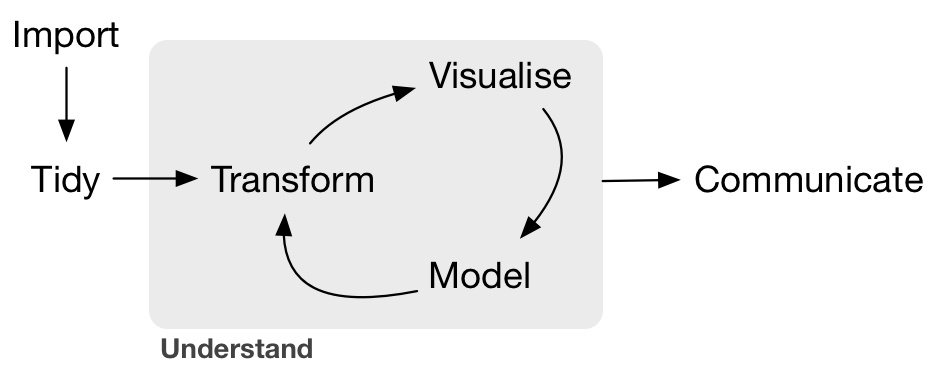
\includegraphics[width=\textwidth]{images/tidy1} 

}

\caption[Hadley's workflow graphic]{Hadley's workflow graphic}\label{fig:unnamed-chunk-3}
\end{figure}

We will begin with a discussion on what is meant by tidy data and then
dig into the gray \textbf{Understand} portion of the cycle and conclude
by talking about interpreting and discussing the results of our models
via \textbf{Communication}. These steps are vital to any statistical
analysis. But why should you care about statistics? ``Why did they make
me take this class?''

There's a reason so many fields require a statistics course. Scientific
knowledge grows through an understanding of statistical significance and
data analysis. You needn't be intimidated by statistics. It's not the
beast that it used to be and, paired with computation, you'll see how
reproducible research in the sciences particularly increases scientific
knowledge.

\section{Reproducibility}\label{reproducibility}

\begin{quote}
``The most important tool is the \emph{mindset}, when starting, that the
end product will be reproducible.'' -- Keith Baggerly
\end{quote}

Another large goal of this book is to help readers understand the
importance of reproducible analyses. The hope is to get readers into the
habit of making their analyses reproducible from the very beginning.
This means we'll be trying to help you build new habits. This will take
practice and be difficult at times. You'll see just why it is so
important for you to keep track of your code and well-document it to
help yourself later and any potential collaborators as well.

Copying and pasting results from one program into a word processor is
not the way that efficient and effective scientific research is
conducted. It's much more important for time to be spent on data
collection and data analysis and not on copying and pasting plots back
and forth across a variety of programs.

In a traditional analyses if an error was made with the original data,
we'd need to step through the entire process again: recreate the plots
and copy and paste all of the new plots and our statistical analysis
into your document. This is error prone and a frustrating use of time.
We'll see how to use R Markdown to get away from this tedious activity
so that we can spend more time doing science.

\begin{quote}
``We are talking about \emph{computational} reproducibility.'' - Yihui
Xie
\end{quote}

Reproducibility means a lot of things in terms of different scientific
fields. Are experiments conducted in a way that another researcher could
follow the steps and get similar results? In this book, we will focus on
what is known as \textbf{computational reproducibility}. This refers to
being able to pass all of one's data analysis, data sets, and
conclusions to someone else and have them get exactly the same results
on their machine. This allows for time to be spent doing actual science
and interpreting of results and assumptions instead of the more error
prone way of starting from scratch or following a list of steps that may
be different from machine to machine.

\section{Who is this book for?}\label{who-is-this-book-for}

This book is targeted at students taking a traditional intro stats class
in a small college environment using RStudio and preferably RStudio
Server. We assume no prerequisites: no algebra, no calculus, and no
prior programming experience. This is intended to be a gentle and nice
introduction to the practice of statistics in terms of how data
scientists, statisticians, data journalists, and other scientists
analyze data and write stories about data. We have intentionally avoided
the use of throwing formulas at you as much as possible and instead have
focused on developing statistical concepts via data visualization and
statistical computing. We hope this is a more intuitive experience than
the way statistics has traditionally been taught in the past (and how it
is commonly perceived from the outside). We additionally hope that you
see the value of reproducible research via R as you continue in your
studies. We understand that there will initially be growing pains in
learning to program but we are here to help you and you should know that
there is a huge community of R users that are always happy to help
newbies along as well.

Now let's get into learning about how to create good stories about and
with data!

\part{Data Exploration}\label{part-data-exploration}

\chapter{Tidy Data}\label{tidy}

In this chapter, we'll discuss the importance of tidy data. You may
think that this means just having your data in a spreadsheet, but you'll
see that it is actually more specific than that. Data actually comes to
us in a variety of formats from pictures to text to just numbers. We'll
focus on datasets that can be stored in a spreadsheet throughout this
book as that is the most common way data is collected in the sciences.

Having tidy data will allow us to more easily create data visualizations
as we will see in Chapter \ref{viz}. It will also help us with
manipulating data in Chapter \ref{manip} and in all subsequent chapters
when we discuss statistical inference. You may not necessarily
understand the importance for \textbf{tidy data} immediately but it will
become more and more apparent as we proceed through the book.

\section{What is tidy data?}\label{what-is-tidy-data}

You have surely heard the word ``tidy'' in your life:

\begin{itemize}
\tightlist
\item
  ``Tidy up your room!''
\item
  ``Please write your homework in a tidy way so that it is easier to
  grade and to provide feedback.''
\item
  Marie Kondo's best-selling book
  \href{https://www.amazon.com/Life-Changing-Magic-Tidying-Decluttering-Organizing/dp/1607747308/ref=sr_1_1?ie=UTF8\&qid=1469400636\&sr=8-1\&keywords=tidying+up}{\emph{The
  Life-Changing Magic of Tidying Up: The Japanese Art of Decluttering
  and Organizing}}
\item
  ``I am not by any stretch of the imagination a tidy person, and the
  piles of unread books on the coffee table and by my bed have a
  plaintive, pleading quality to me - `Read me, please!'\,'' - Linda
  Grant
\end{itemize}

So what does it mean for your data to be \textbf{tidy}? Put simply, it
means that your data is organized. But it's more than just that. It
means that your data follows the same standard format making it easy for
others to find elements of your data, to manipulate and transform your
data, and, for our purposes, continuing with the common theme: it makes
it easier to visualize your data and the relationships between different
variables in your data.

We will follow Hadley Wickham's definition of \textbf{tidy data} here
\citep{tidy}:

\begin{quote}
A dataset is a collection of values, usually either numbers (if
quantitative) or strings (if qualitative). Values are organised in two
ways. Every value belongs to a variable and an observation. A variable
contains all values that measure the same underlying attribute (like
height, temperature, duration) across units. An observation contains all
values measured on the same unit (like a person, or a day, or a race)
across attributes.
\end{quote}

\begin{quote}
Tidy data is a standard way of mapping the meaning of a dataset to its
structure. A dataset is messy or tidy depending on how rows, columns and
tables are matched up with observations, variables and types. In
\textbf{tidy data}:
\end{quote}

\begin{quote}
\begin{enumerate}
\def\labelenumi{\arabic{enumi}.}
\tightlist
\item
  Each variable forms a column.
\item
  Each observation forms a row.
\item
  Each type of observational unit forms a table.
\end{enumerate}
\end{quote}

\begin{figure}

{\centering 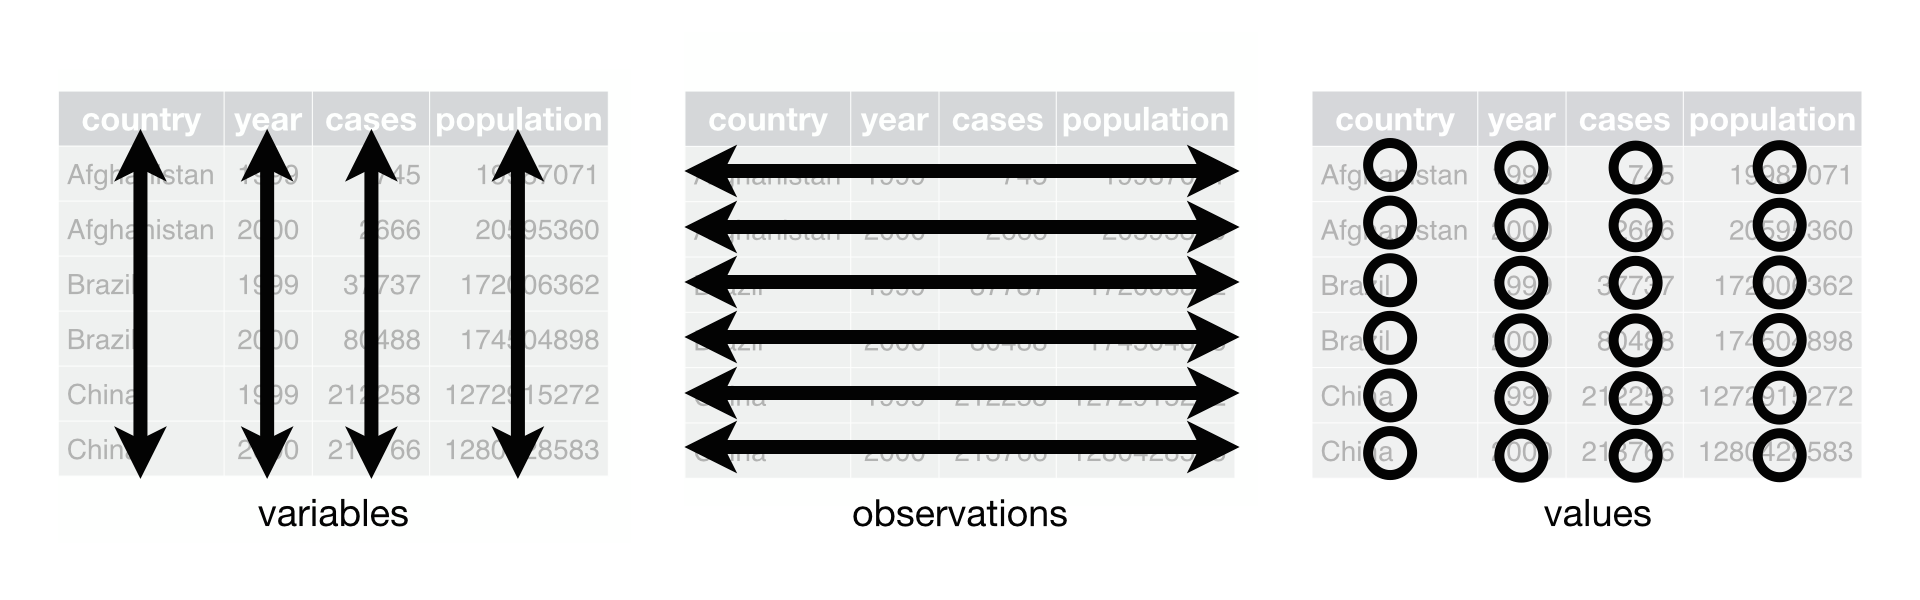
\includegraphics[width=\textwidth]{images/tidy-1} 

}

\caption[Tidy data graphic from http://r4ds.had.co.nz/tidy-data.html]{Tidy data graphic from http://r4ds.had.co.nz/tidy-data.html}\label{fig:tidyfig}
\end{figure}

Reading over this definition, you can begin to think about datasets that
won't follow this nice format.

\begin{center}\rule{0.5\linewidth}{\linethickness}\end{center}

\begin{learncheck}
\textbf{\emph{Learning check}}
\end{learncheck}

\textbf{(LC3.1)} Give an example dataset that doesn't follow this
format.

\begin{itemize}
\tightlist
\item
  What features of this dataset might make it difficult to visualize?\\
\item
  How could the dataset be tweaked to make it \textbf{tidy}?
\end{itemize}

\begin{center}\rule{0.5\linewidth}{\linethickness}\end{center}

\section{\texorpdfstring{The \texttt{nycflights13}
datasets}{The nycflights13 datasets}}\label{the-nycflights13-datasets}

We likely have all flown on airplanes or know someone that has. Air
travel has become an ever-present aspect of our daily lives. If you live
in or are visiting a relatively large city and you walk around that
city's airport, you see gates showing flight information from many
different airlines. And you will frequently see that some flights are
delayed because of a variety of conditions. Are there ways that we can
avoid having to deal with these flight delays?

We'd all like to arrive at our destinations on time whenever possible.
(Unless you secretly love hanging out at airports. If you are one of
these people, pretend for the moment that you are very much anticipating
being at your final destination.) Hadley Wickham (herein just referred
to as ``Hadley'') created multiple datasets containing information about
departing flights from the New York City area in 2013
\citep{R-nycflights13}. We will begin by loading in one of these
datasets, the \texttt{flights} dataset, and getting an idea of its
structure:

\begin{Shaded}
\begin{Highlighting}[]
\KeywordTok{library}\NormalTok{(nycflights13)}
\KeywordTok{data}\NormalTok{(flights)}
\end{Highlighting}
\end{Shaded}

The \texttt{library} function here loads the R package
\texttt{nycflights13} into the current R environment in which you are
working. The \texttt{data(flights)} loads in the \texttt{flights}
dataset that is stored in the \texttt{nycflights13} package. Note that
you'll get an error if you try to load this package in and it hasn't
been downloaded and installed. You can ensure it is installed by running
the code below:

\begin{Shaded}
\begin{Highlighting}[]
\NormalTok{if(!}\KeywordTok{require}\NormalTok{(nycflights13))}
  \KeywordTok{install.packages}\NormalTok{(}\StringTok{"nycflights13"}\NormalTok{, }\DataTypeTok{repos =} \StringTok{"http://cran.rstudio.org"}\NormalTok{)}
\end{Highlighting}
\end{Shaded}

This code checks to see if \texttt{nycflights13} is installed and, if
not, then goes to the specified repository of
``\url{http://cran.rstudio.org}'' and downloads the package from there
and installs it. If it is already installed you can see it listed in the
\textbf{Packages} tab in the bottom right portion of RStudio and the
code will not install the package again since this is redundant and you
won't need to do it over and over again.

This dataset and most others presented in this book will be in the
\texttt{data.frame} format in R. Data frames are ways to look at
collections of variables that are tightly coupled together. Frequently,
the best way to get a feel for a data frame is to use the \texttt{View}
function in RStudio. This command will be given throughout the book as a
reminder, but the actual output will be hidden. Run
\texttt{View(flights)} in R and look over this data frame.

\begin{center}\rule{0.5\linewidth}{\linethickness}\end{center}

\begin{learncheck}
\textbf{\emph{Learning check}}
\end{learncheck}

\textbf{(LC3.2)} What does any \emph{ONE} row in this \texttt{flights}
dataset refer to?

\begin{itemize}
\tightlist
\item
  A. Data on an airline
\item
  B. Data on a flight
\item
  C. Data on an airport
\item
  D. Data on multiple flights
\end{itemize}

\begin{center}\rule{0.5\linewidth}{\linethickness}\end{center}

By running \texttt{View(flights)}, we see the different
\textbf{variables} listed in the columns and we see that there are
different types of variables. Some of the variables like
\texttt{distance}, \texttt{day}, and \texttt{arr\_delay} are what we
will call \textbf{quantitative} variables. These variables vary in a
numerical way. Other variables here are \textbf{categorical}.

Note that if you look in the leftmost column of the
\texttt{View(flights)} output, you will see a column of numbers. These
are the row numbers of the dataset. If you glance across a row with the
same number, say row 5, you can get an idea of what each row corresponds
to. In other words, this will allow you to identify what object is being
referred to in a given row. This is often called the
\textbf{observational unit}. The \textbf{observational unit} in this
example is an individual flight departing New York City in 2013. You can
identify the observational unit by determining what the \textbf{thing}
is that is being measured in each of the variables.

\textbf{Note}: Frequently the first thing you should do when given a
dataset is to

\begin{itemize}
\tightlist
\item
  identify the observation unit,
\item
  specify the variables, and
\item
  give the types of variables you are presented with.
\end{itemize}

\begin{Shaded}
\begin{Highlighting}[]
\KeywordTok{str}\NormalTok{(flights)}
\end{Highlighting}
\end{Shaded}

\begin{verbatim}
## Classes 'tbl_df', 'tbl' and 'data.frame':    336776 obs. of  19 variables:
##  $ year          : int  2013 2013 2013 2013 2013 2013 2013 2013 2013 2013 ...
##  $ month         : int  1 1 1 1 1 1 1 1 1 1 ...
##  $ day           : int  1 1 1 1 1 1 1 1 1 1 ...
##  $ dep_time      : int  517 533 542 544 554 554 555 557 557 558 ...
##  $ sched_dep_time: int  515 529 540 545 600 558 600 600 600 600 ...
##  $ dep_delay     : num  2 4 2 -1 -6 -4 -5 -3 -3 -2 ...
##  $ arr_time      : int  830 850 923 1004 812 740 913 709 838 753 ...
##  $ sched_arr_time: int  819 830 850 1022 837 728 854 723 846 745 ...
##  $ arr_delay     : num  11 20 33 -18 -25 12 19 -14 -8 8 ...
##  $ carrier       : chr  "UA" "UA" "AA" "B6" ...
##  $ flight        : int  1545 1714 1141 725 461 1696 507 5708 79 301 ...
##  $ tailnum       : chr  "N14228" "N24211" "N619AA" "N804JB" ...
##  $ origin        : chr  "EWR" "LGA" "JFK" "JFK" ...
##  $ dest          : chr  "IAH" "IAH" "MIA" "BQN" ...
##  $ air_time      : num  227 227 160 183 116 150 158 53 140 138 ...
##  $ distance      : num  1400 1416 1089 1576 762 ...
##  $ hour          : num  5 5 5 5 6 5 6 6 6 6 ...
##  $ minute        : num  15 29 40 45 0 58 0 0 0 0 ...
##  $ time_hour     : POSIXct, format: "2013-01-01 05:00:00" ...
\end{verbatim}

\begin{center}\rule{0.5\linewidth}{\linethickness}\end{center}

\begin{learncheck}
\textbf{\emph{Learning check}}
\end{learncheck}

\textbf{(LC3.3)} What are some examples in this dataset of
\textbf{categorical} variables? What makes them different than
\textbf{quantitative} variables?

\textbf{(LC3.4)} What does \texttt{int}, \texttt{num}, and \texttt{chr}
mean in the output above?

\textbf{(LC3.5)} How many different columns are in this dataset?

\textbf{(LC3.6)} How many different rows are in this dataset?

\begin{center}\rule{0.5\linewidth}{\linethickness}\end{center}

Another way to view the properties of a dataset is to use the
\texttt{str} function (``str'' is short for ``structure''). The
\texttt{str} function is expecting an object for its argument. In this
case, the object is a data frame named \texttt{flights}. You can use the
\texttt{str} function on other objects and data frames using the syntax
\texttt{str(object)} where \texttt{object} is the name of an object in
R. This will give you the first few entries of each variable in a row
after the variable. In addition, the type of the variable is given
immediately after the \texttt{:} following each variable's name. Here,
\texttt{int} and \texttt{num} refer to quantitative variables. In
contrast, \texttt{chr} refers to categorical variables. One more type of
variable is given here with the \texttt{time\_hour} variable:
\textbf{POSIXct}. As you may suspect, this variable corresponds to a
specific date and time of day.

Another nice feature of R is the help system. You can get help in R by
simply entering a question mark before the name of a function or an
object and you will be presented with a page showing the documentation.
Note that this output help file is omitted here but can be accessed
\href{https://cran.r-project.org/web/packages/nycflights13/nycflights13.pdf}{here}
on page 3 of the PDF document.

\begin{Shaded}
\begin{Highlighting}[]
\NormalTok{?str}
\NormalTok{?flights}
\end{Highlighting}
\end{Shaded}

Another aspect of tidy data is a description of what each variable in
the dataset represents. This helps others to understand what your
variable names mean and what they correspond to. If we look at the
output of \texttt{?flights}, we can see that a description of each
variable by name is given.

An important feature to \textbf{ALWAYS} include with your data is the
appropriate units of measurement. We'll see this further when we work
with the \texttt{dep\_delay} variable in Chapter \ref{viz}. (It's in
minutes, but you'd get some really strange interpretations if you
thought it was in hours or seconds. UNITS MATTER!)

\section{\texorpdfstring{How is \texttt{flights}
tidy?}{How is flights tidy?}}\label{how-is-flights-tidy}

We see that \texttt{flights} has a rectangular shape with each row
corresponding to a different flight and each column corresponding to a
characteristic of that flight. This matches exactly with how Hadley
defined tidy data:

\begin{enumerate}
\def\labelenumi{\arabic{enumi}.}
\tightlist
\item
  Each variable forms a column.
\item
  Each observation forms a row.
\end{enumerate}

But what about the third property?

\begin{quote}
\begin{enumerate}
\def\labelenumi{\arabic{enumi}.}
\setcounter{enumi}{2}
\tightlist
\item
  Each type of observational unit forms a table.
\end{enumerate}
\end{quote}

We identified earlier that the observational unit in the
\texttt{flights} dataset is an individual flight. And we have shown that
this dataset consists of 336,776 flights with 19 variables. In other
words, some rows of this dataset don't refer to a measurement on an
airline or on an airport. They specifically refer to
characteristics/measurements on a given \textbf{flight} from New York
City in 2013.

By contrast, also included in the \texttt{nycflights13} package are
datasets with different observational units \citep{R-nycflights13}:

\begin{itemize}
\tightlist
\item
  \texttt{weather}: hourly meteorological data for each airport
\item
  \texttt{planes}: construction information about each plane
\item
  \texttt{airports}: airport names and locations
\item
  \texttt{airlines}: translation between two letter carrier codes and
  names
\end{itemize}

You may have been asking yourself what \texttt{carrier} refers to in the
\texttt{str(flights)} output above. The \texttt{airlines} dataset
provides a description of this with each airline being the observational
unit:

\begin{Shaded}
\begin{Highlighting}[]
\KeywordTok{data}\NormalTok{(airlines)}
\NormalTok{airlines}
\end{Highlighting}
\end{Shaded}

\begin{verbatim}
##    carrier                        name
## 1       9E           Endeavor Air Inc.
## 2       AA      American Airlines Inc.
## 3       AS        Alaska Airlines Inc.
## 4       B6             JetBlue Airways
## 5       DL        Delta Air Lines Inc.
## 6       EV    ExpressJet Airlines Inc.
## 7       F9      Frontier Airlines Inc.
## 8       FL AirTran Airways Corporation
## 9       HA      Hawaiian Airlines Inc.
## 10      MQ                   Envoy Air
## 11      OO       SkyWest Airlines Inc.
## 12      UA       United Air Lines Inc.
## 13      US             US Airways Inc.
## 14      VX              Virgin America
## 15      WN      Southwest Airlines Co.
## 16      YV          Mesa Airlines Inc.
\end{verbatim}

As can be seen here when you just enter the name of an object in R, by
default it will print the contents of that object to the screen. Be
careful! It's usually better to use the \texttt{View()} function in
RStudio since larger objects may take awhile to print to the screen and
it likely won't be helpful to you to have hundreds of lines outputted.

\section{Normal forms of data}\label{normal-forms-of-data}

The datasets included in the \texttt{nycflights13} package are in a form
that minimizes redundancy of data. We will see that there are ways to
\emph{merge} (or \emph{join}) the different tables together easily. We
are capable of doing so because each of the tables have \emph{keys} in
common to relate one to another. This is an important property of
\textbf{normal forms} of data. The process of decomposing data frames
into less redundant tables without losing information is called
\textbf{normalization}. More information is available on
\href{https://en.wikipedia.org/wiki/Database_normalization}{Wikipedia}.

We saw an example of this above with the \texttt{airlines} dataset.
While the \texttt{flights} data frame could also include a column with
the names of the airlines instead of the carrier code, this would be
repetitive since there is a unique mapping of the carrier code to the
name of the airline/carrier.

Below an example is given showing how to \textbf{join} the
\texttt{airlines} data frame together with the \texttt{flights} data
frame by linking together the two datasets via a common \textbf{key} of
\texttt{"carrier"}. Note that this ``joined'' data frame is assigned to
a new data frame called \texttt{joined\_flights}.

\begin{Shaded}
\begin{Highlighting}[]
\NormalTok{if(!}\KeywordTok{require}\NormalTok{(nycflights13))}
  \KeywordTok{install.packages}\NormalTok{(}\StringTok{"nycflights13"}\NormalTok{, }\DataTypeTok{repos =} \StringTok{"http://cran.rstudio.org"}\NormalTok{)}
\KeywordTok{library}\NormalTok{(dplyr)}
\NormalTok{joined_flights <-}\StringTok{ }\KeywordTok{inner_join}\NormalTok{(}\DataTypeTok{x =} \NormalTok{flights, }\DataTypeTok{y =} \NormalTok{airlines, }\DataTypeTok{by =} \StringTok{"carrier"}\NormalTok{)}
\end{Highlighting}
\end{Shaded}

\begin{Shaded}
\begin{Highlighting}[]
\KeywordTok{View}\NormalTok{(joined_flights)}
\end{Highlighting}
\end{Shaded}

If we \texttt{View} this dataset, we see a new variable has been created
called (We will see in Subsection 5.1.1 ways to change \texttt{name} to
a more descriptive variable name.)

More discussion about joining data frames together will be given in
Chapter \ref{manip}. We will see there that the names of the columns to
be linked need not match as they did here with \texttt{"carrier"}.

\begin{center}\rule{0.5\linewidth}{\linethickness}\end{center}

\begin{center}\rule{0.5\linewidth}{\linethickness}\end{center}

\begin{review}
\textbf{\emph{Review questions}}
\end{review}

\textbf{(RQ3.1)} What are common characteristics of ``tidy'' datasets?

\textbf{(RQ3.2)} What makes ``tidy'' datasets useful for organizing
data?

\textbf{(RQ3.3)} How many variables are presented in the table below?
What does each row correspond to? (\textbf{Hint:} You may not be able to
answer both of these questions immediately but take your best guess.)

\begin{tabular}{r|r}
\hline
students & faculty\\
\hline
4 & 2\\
\hline
6 & 3\\
\hline
\end{tabular}

\textbf{(RQ3.4)} The confusion you may have encountered in Question 4 is
a common one those that work with data are commonly presented with. This
dataset is not tidy. Actually, the dataset in Question 4 has three
variables not the two that were presented. Make a guess as to what these
variables are and present a tidy dataset instead of this untidy one
given in Question 4.

\textbf{(RQ3.5)} The actual data presented in Question 4 is given below
in tidy data format:

\begin{tabular}{l|l|l}
\hline
role & Sociology? & Type of School\\
\hline
student & TRUE & Public\\
\hline
student & TRUE & Public\\
\hline
student & TRUE & Public\\
\hline
student & TRUE & Public\\
\hline
student & FALSE & Public\\
\hline
student & FALSE & Public\\
\hline
student & FALSE & Private\\
\hline
student & FALSE & Private\\
\hline
student & FALSE & Private\\
\hline
student & FALSE & Private\\
\hline
faculty & TRUE & Public\\
\hline
faculty & TRUE & Public\\
\hline
faculty & FALSE & Public\\
\hline
faculty & FALSE & Private\\
\hline
faculty & FALSE & Private\\
\hline
\end{tabular}

\begin{itemize}
\tightlist
\item
  What does each row correspond to?\\
\item
  What are the different variables in this data frame?\\
\item
  The \texttt{Sociology?} variable is known as a logical variable. What
  types of values does a logical variable take on?
\end{itemize}

\textbf{(RQ3.6)} What are some advantages of data in normal forms? What
are some disadvantages?

\begin{center}\rule{0.5\linewidth}{\linethickness}\end{center}

\begin{center}\rule{0.5\linewidth}{\linethickness}\end{center}

\section{What's to come?}\label{whats-to-come}

In Chapter \ref{viz}, we will further explore the distribution of a
variable in a related dataset to \texttt{flights}: the \texttt{temp}
variable in the \texttt{weather} dataset. We'll be interested in
understanding how this variable varies in relation to the values of
other variables in the dataset. We will see that visualization is often
a powerful tool in helping us see what is going on in a dataset. It will
be a useful way to expand on the \texttt{str} function we have seen here
for tidy data.

\chapter{Data Visualization via ggplot2}\label{viz}

In Chapter \ref{tidy}, we discussed the importance of datasets being
\textbf{tidy}. You will see in examples here why having a tidy dataset
helps us immensely when plotting our data. In plotting our data, we will
be able to gain valuable insights from our data that we couldn't
initially see from just looking at the raw data. We will focus on using
Hadley Wickham's \texttt{ggplot2} package in doing so, which was
developed to work specifically on datasets that are \textbf{tidy}. It
provides an easy way to customize your plots and is based on data
visualization theory given in \emph{The Grammar of Graphics}
\citep{wilkinson2005}.

At the most basic level, graphics/plots/charts provide a nice way for us
to get a sense for how quantitative variables compare in terms of their
center and their spread. The most important thing to know about graphics
is that they should be created to make it obvious for your audience to
see the findings you want to get across. This requires a balance of not
including too much in your plots, but also including enough so that
relationships and interesting findings can be easily seen. As we will
see, plots/graphics also help us to identify patterns and outliers in
our data. We will see that a common extension of these ideas is to
compare the \textbf{distribution} of one quantitative variable (i.e.,
what the spread of a variable looks like or how the variable is
\emph{distributed} in terms of its values) as we go across the levels of
a different categorical variable.

\section*{Needed packages}\label{needed-packages}
\addcontentsline{toc}{section}{Needed packages}

Before we proceed with this chapter, let's load all the necessary
packages, in particular the \texttt{nycflights13} package introduced in
Chapter \ref{tidy} containing various data sets.

\begin{Shaded}
\begin{Highlighting}[]
\KeywordTok{library}\NormalTok{(ggplot2)}
\KeywordTok{library}\NormalTok{(nycflights13)}
\KeywordTok{library}\NormalTok{(knitr)}
\KeywordTok{library}\NormalTok{(dplyr)}
\end{Highlighting}
\end{Shaded}

\section{The Grammar of Graphics}\label{grammarofgraphics}

We begin with a discussion of a theoretical framework for data
visualization known as the ``The Grammar of Graphics,'' which serves as
the basis for the \texttt{ggplot2} package. Much like the way we
construct sentences in any language using a linguistic grammar (nouns,
verbs, subjects, objects, etc.), the theoretical framework given by
Leland Wilkinson \citep{wilkinson2005} allows us to specify the
components of a statistical graphic.

\subsection{Components of Grammar}\label{components-of-grammar}

In short, the grammar tells us that:

\begin{quote}
\textbf{A statistical graphic is a mapping of \texttt{data} variables to
\texttt{aes}thetic attributes of \texttt{geom}etric objects.}
\end{quote}

Specifically, we can break a graphic into the following three essential
components:

\begin{enumerate}
\def\labelenumi{\arabic{enumi}.}
\tightlist
\item
  \texttt{data}: the data set comprised of variables that we map.
\item
  \texttt{geom}: the geometric object in question. This refers to our
  type of objects we can observe in our plot. For example, points,
  lines, bars, etc.
\item
  \texttt{aes}: aesthetic attributes of the geometric object that we can
  perceive on a graphic. For example, x/y position, color, shape, and
  size. Each assigned aesthetic attribute can be mapped to a variable in
  our data set. If not assigned, they are set to defaults.
\end{enumerate}

\subsection{Napolean's March on Moscow}\label{napoleans-march-on-moscow}

In 1812, Napoleon led a French invasion of Russia, marching on Moscow.
It was one of the biggest military disasters due in large part to the
Russian winter. In 1869, a French civil engineer named Charles Joseph
Minard published arguably one of the greatest statistical visualizations
of all-time, which summarized this march:

\begin{figure}

{\centering 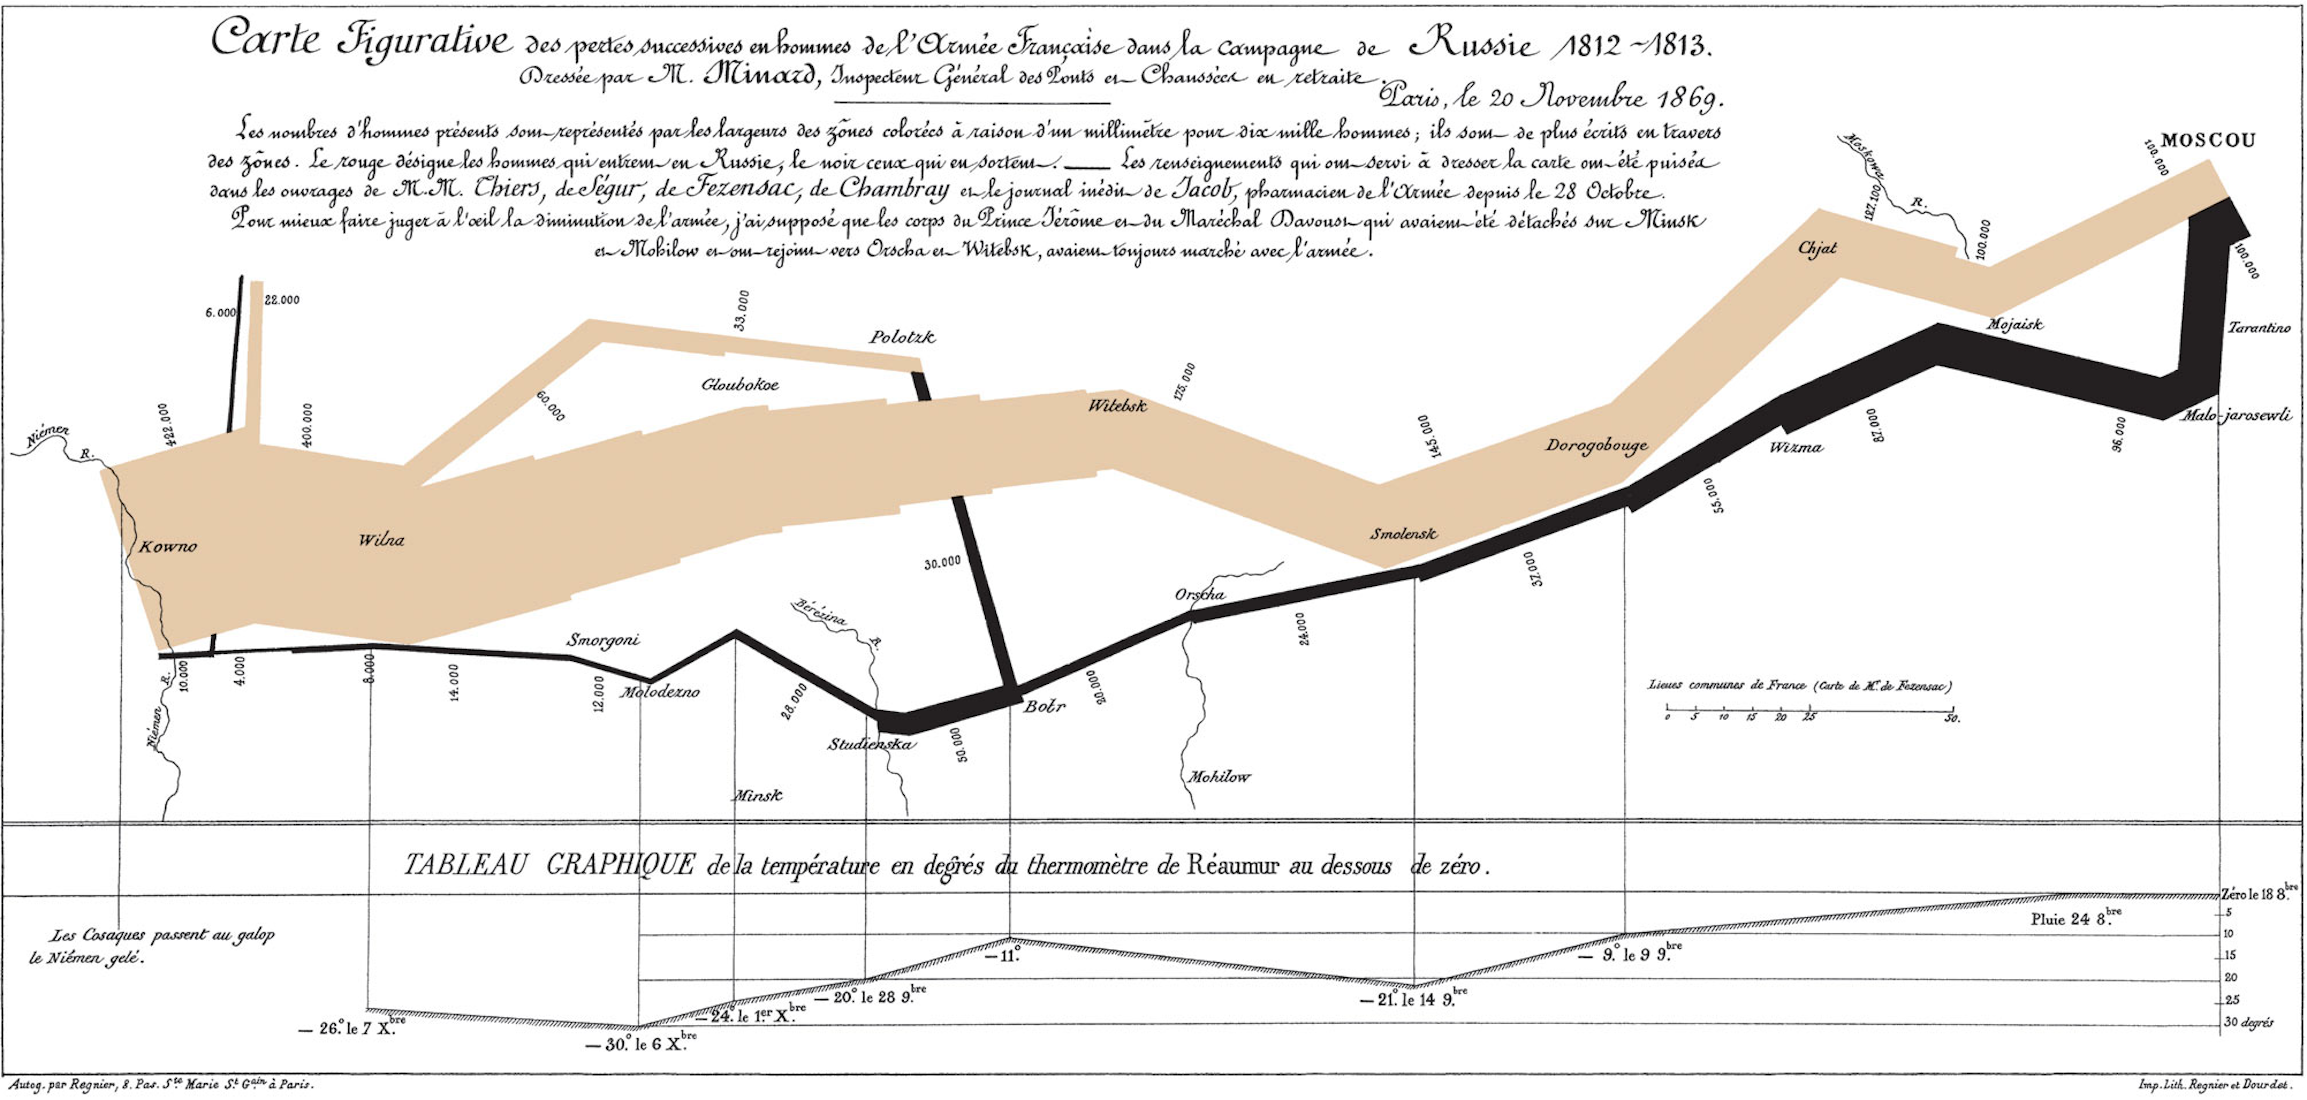
\includegraphics[width=\textwidth]{images/Minard} 

}

\caption[Minard's Visualization of Napolean's March]{Minard's Visualization of Napolean's March}\label{fig:minard}
\end{figure}

This was considered a revolution in statistical graphics because between
the map on top and the line graph on the bottom, there are 6 dimensions
of information (i.e.~variables) being displayed on a 2-dimensional page.
Let's view this graphic through the lens of the Grammar of Graphics:

\begin{table}
\caption{\label{tab:unnamed-chunk-12}Grammar of Map (Top) and Line-Graph (Bottom) in Minard's Graphic of Napolean's March}

\centering
\begin{tabular}[t]{lll}
\toprule
data & aes & geom\\
\midrule
longitude & x & point\\
latitude & y & point\\
army size & size & path\\
army direction & color & path\\
\bottomrule
\end{tabular}
\centering
\begin{tabular}[t]{lll}
\toprule
data & aes & geom\\
\midrule
date & x & line \& text\\
temperature & y & line \& text\\
\bottomrule
\end{tabular}
\end{table}

For example, the data variable \texttt{longitude} gets mapped to the
\texttt{x} \texttt{aes}thetic of the points \texttt{geom}etric objects
on the map while the annotated line-graph displays \texttt{date} and
\texttt{temperature} variable information via its mapping to the
\texttt{x} and \texttt{y} \texttt{aes}thetic of the line
\texttt{geom}etric object.

\subsection{Other Components of the
Grammar}\label{other-components-of-the-grammar}

There are other components of the Grammar of Graphics we can control:

\begin{itemize}
\tightlist
\item
  \texttt{facet}: how to break up a plot into subsets
\item
  \texttt{stat}istical transformations: this includes smoothing, binning
  values into a histogram, or just itself un-transformed as
  \texttt{"identity"}.
\item
  \texttt{scales} both

  \begin{itemize}
  \tightlist
  \item
    convert \textbf{data units} to \textbf{physical units} the computer
    can display
  \item
    draw a legend and/or axes, which provide an inverse mapping to make
    it possible to read the original data values from the graph.
  \end{itemize}
\item
  \texttt{coord}inate system for x/y values: typically
  \texttt{cartesian}, but can also be \texttt{polar} or \texttt{map}
\item
  \texttt{position} adjustments
\end{itemize}

In this text, we will only focus on the first two: \texttt{facet}ing
(introduced in Section \ref{facets}) and \texttt{stat}istical
transformations (in a limited sense, when consider Barplots in Section
\ref{geombar}); the other components are left to a more advanced text.
This is not a problem when producing a plot as each of these components
have default settings.

There are other extra attributes that can be tweaked as well including
the plot title, axes labels, and over-arching themes for the plot. In
general, the Grammar of Graphics allows for customization but also a
consistent framework that allows the user to easily tweak their
creations as needed in order to convey a message about their data.

\subsection{\texorpdfstring{The \texttt{ggplot2}
Package}{The ggplot2 Package}}\label{the-ggplot2-package}

We next introduce Hadley Wickham's \texttt{ggplot2} package, which is an
implementation of the Grammar of Graphics for R \citep{R-ggplot2}. You
may have noticed that a lot of previous text in this chapter is written
in computer font. This is because the various components of the Grammar
of Graphics are specified using the \texttt{ggplot} function, which
expects at a bare minimal as arguments

\begin{itemize}
\tightlist
\item
  the data frame where the variables exist (the \texttt{data} argument)
  and
\item
  the names of the variables to be plotted (the \texttt{mapping}
  argument).
\end{itemize}

The names of the variables will be entered into the \texttt{aes}
function as arguments where \texttt{aes} stands for ``aesthetics''.

\section{Five Named Graphs - The 5NG}\label{five-named-graphs---the-5ng}

For our purposes, we will be limiting consideration to five different
types of graphs (note that in this text we use the terms ``graphs'',
``plots'', and ``charts'' interchangeably). We term these five named
graphs the \textbf{5NG}:

\begin{enumerate}
\def\labelenumi{\arabic{enumi}.}
\tightlist
\item
  scatter-plots
\item
  line-graphs
\item
  boxplots
\item
  histograms
\item
  barplots
\end{enumerate}

With this repertoire of plots, you can visualize a wide array of data
variables thrown at you. We will discuss some variations of these, but
with the 5NG in your toolbox you can do big things! Something we will
also stress here is that certain plots only work for categorical/logical
variables and others only for quantitative variables. You'll want to
quiz yourself often as we go along on which plot makes sense a given a
particular problem set-up.

\section{5NG\#1: Scatter-plots}\label{scatterplots}

The simplest of the 5NG are \textbf{scatter-plots} (also called
bivariate plots); they allow you to investigate the relationship between
two continuous variables. While you may already be familiar with such
plots, let's view it through the lens of the Grammar of Graphics.
Specifically, we will graphically investigate the relationship between
the following two continuous variables in the \texttt{flights} data
frame:

\begin{enumerate}
\def\labelenumi{\arabic{enumi}.}
\tightlist
\item
  \texttt{dep\_delay}: departure delay on the horizontal ``x'' axis and
\item
  \texttt{arr\_delay}: arrival delay on the vertical ``y'' axis
\end{enumerate}

for Alaska Airlines flights leaving NYC in 2013. This requires paring
down the \texttt{flights} data frame to a smaller data frame
\texttt{all\_alaska\_flights} consisting of only Alaska Airlines
(carrier code ``AS'') flights.

\begin{Shaded}
\begin{Highlighting}[]
\KeywordTok{data}\NormalTok{(flights)}
\NormalTok{all_alaska_flights <-}\StringTok{ }\NormalTok{flights %>%}\StringTok{ }
\StringTok{  }\KeywordTok{filter}\NormalTok{(carrier ==}\StringTok{ "AS"}\NormalTok{)}
\end{Highlighting}
\end{Shaded}

This code snippet makes use of functions in the \texttt{dplyr} package
for data manipulation to achieve our goal: it takes the \texttt{flights}
data frame and \texttt{filter}s it to only return the rows which meet
the condition \texttt{carrier\ ==\ "AS"} (recall equality is specified
with \texttt{==} and not \texttt{=}). You will see many more examples
using this function in Chapter \ref{manip}.

\begin{center}\rule{0.5\linewidth}{\linethickness}\end{center}

\begin{learncheck}
\textbf{\emph{Learning check}}
\end{learncheck}

\textbf{(LC4.1)} Take a look at both the \texttt{flights} and
\texttt{all\_alaska\_flights} data frames by running
\texttt{View(flights)} and \texttt{View(all\_alaska\_flights)} in the
console. In what respect do these data frames differ?

\begin{center}\rule{0.5\linewidth}{\linethickness}\end{center}

\subsection{\texorpdfstring{Scatter-plots via
\texttt{geom\_point}}{Scatter-plots via geom\_point}}\label{scatter-plots-via-geom_point}

We proceed to create the scatter-plot using the \texttt{ggplot()}
function:

\begin{Shaded}
\begin{Highlighting}[]
\KeywordTok{ggplot}\NormalTok{(}\DataTypeTok{data =} \NormalTok{all_alaska_flights, }\KeywordTok{aes}\NormalTok{(}\DataTypeTok{x =} \NormalTok{dep_delay, }\DataTypeTok{y =} \NormalTok{arr_delay)) +}\StringTok{ }
\StringTok{  }\KeywordTok{geom_point}\NormalTok{()}
\end{Highlighting}
\end{Shaded}

\begin{figure}

{\centering 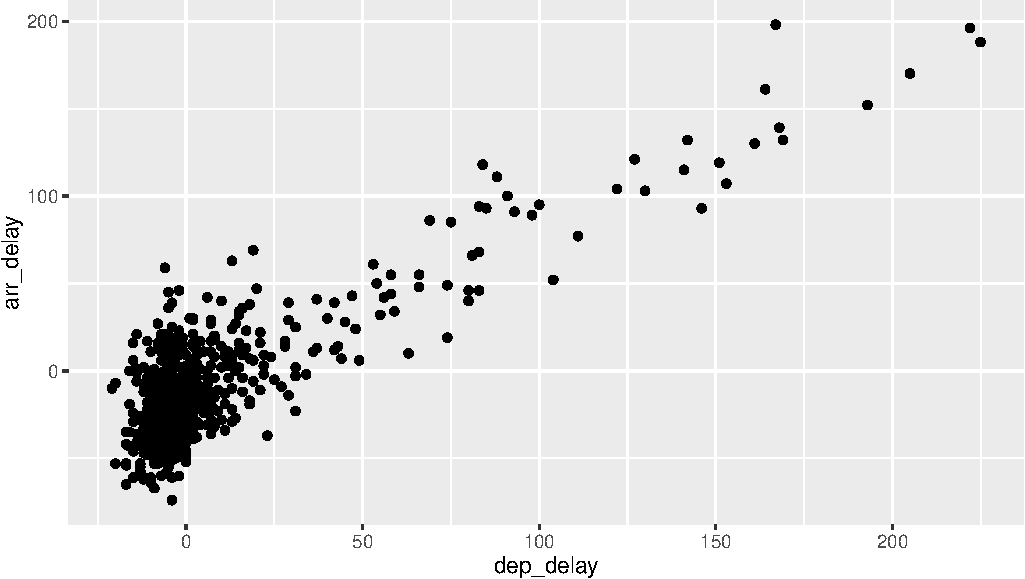
\includegraphics[width=\textwidth]{ismaykim_files/figure-latex/noalpha-1} 

}

\caption[Arrival Delays vs Departure Delays for Alaska Airlines flights from NYC in 2013]{Arrival Delays vs Departure Delays for Alaska Airlines flights from NYC in 2013}\label{fig:noalpha}
\end{figure}

You are encouraged to enter \textbf{Return} on your keyboard after
entering the \texttt{+}. As we add more and more elements, it will be
nice to keep them indented as you see below. Note that this will not
work if you begin the line with the \texttt{+}.

Let's break down this keeping in mind our discussion in Section
\ref{grammarofgraphics}:

\begin{itemize}
\tightlist
\item
  Within the \texttt{ggplot()} function call, we specify two of the
  components of the grammar:

  \begin{enumerate}
  \def\labelenumi{\arabic{enumi}.}
  \tightlist
  \item
    The \texttt{data} frame to be \texttt{all\_alaska\_flights} by
    setting \texttt{data\ =\ all\_alaska\_flights}
  \item
    The \texttt{aes}thetic mapping by setting
    \texttt{aes(x\ =\ dep\_delay,\ y\ =\ arr\_delay)}. Specifically

    \begin{itemize}
    \tightlist
    \item
      \texttt{dep\_delay} maps to the \texttt{x} position
    \item
      \texttt{arr\_delay} maps to the \texttt{y} position
    \end{itemize}
  \end{enumerate}
\item
  We add a \textbf{layer} to the \texttt{ggplot()} function call using
  the \texttt{+} sign
\item
  The layer in question specifies the third component of the grammar:
  the \texttt{geom}etric object in question. In this case the geometric
  object are \texttt{point}s, set by specifying \texttt{geom\_point()}
\end{itemize}

In Figure \ref{fig:noalpha} we see that a positive relationship exists
between \texttt{dep\_delay} and \texttt{arr\_delay}: as departure delays
increase, arrival delays tend to also increase. We also note that the
majority of points fall near the point (0, 0). There is a large mass of
points clustered there. (We will work more with this data set in Chapter
\ref{regress}, where we investigate correlation and linear regression.)

\begin{center}\rule{0.5\linewidth}{\linethickness}\end{center}

\begin{learncheck}
\textbf{\emph{Learning check}}
\end{learncheck}

\textbf{(LC4.2)} What are some practical reasons why \texttt{dep\_delay}
and \texttt{arr\_delay} have a positive relationship?

\textbf{(LC4.3)} What variables (not necessarily in the \texttt{flights}
data frame) would you expect to have a negative correlation (i.e.~a
negative relationship) with \texttt{dep\_delay}? Why? Remember that we
are focusing on continuous variables here.

\textbf{(LC4.4)} Why do you believe there is a cluster of points near
(0, 0)? What does (0, 0) correspond to in terms of the Alaskan flights?

\textbf{(LC4.5)} What are some other features of the plot that stand out
to you?

\textbf{(LC4.6)} Create a new scatter-plot using different variables in
the \texttt{all\_alaska\_flights} data frame by modifying the example
above.

\begin{center}\rule{0.5\linewidth}{\linethickness}\end{center}

\subsection{Over-Plotting}\label{over-plotting}

The large mass of points near (0, 0) can cause some confusion. This is
the result of a phenomenon called \textbf{over-plotting}. As one may
guess, this corresponds to values being plotted on top of each other
\emph{over} and \emph{over} again. It is often difficult to know just
how many values are plotted in this way when looking at a basic
scatter-plot as we have here. There are two ways to address this issue:

\begin{enumerate}
\def\labelenumi{\arabic{enumi}.}
\tightlist
\item
  By adjusting the transparency of the points via the \texttt{alpha}
  argument
\item
  By jittering the points via \texttt{geom\_jitter()}
\end{enumerate}

The first way of relieving over-plotting is by changing the
\texttt{alpha} argument to \texttt{geom\_point()} which controls the
transparency of the points. By default, this value is set to \texttt{1}.
We can change this value to a smaller fraction (greater than 0) to
change the transparency of the points in the plot:

\begin{Shaded}
\begin{Highlighting}[]
\KeywordTok{ggplot}\NormalTok{(}\DataTypeTok{data =} \NormalTok{all_alaska_flights, }\KeywordTok{aes}\NormalTok{(}\DataTypeTok{x =} \NormalTok{dep_delay, }\DataTypeTok{y =} \NormalTok{arr_delay)) +}\StringTok{ }
\StringTok{  }\KeywordTok{geom_point}\NormalTok{(}\DataTypeTok{alpha =} \FloatTok{0.2}\NormalTok{)}
\end{Highlighting}
\end{Shaded}

\begin{figure}

{\centering 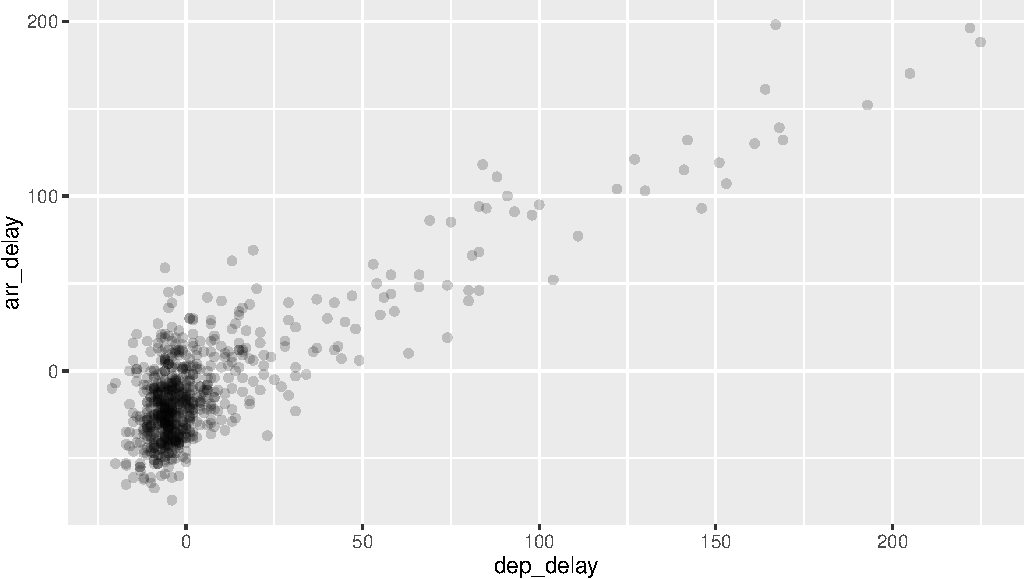
\includegraphics[width=\textwidth]{ismaykim_files/figure-latex/alpha-1} 

}

\caption[Delay scatterplot with alpha=0.2]{Delay scatterplot with alpha=0.2}\label{fig:alpha}
\end{figure}

Note how this function call is identical to the one in Section
\ref{scatterplots}, but with \texttt{geom\_point()} replaced with
\texttt{alpha\ =\ 0.2} added.

The second way of relieving over-plotting is to \textbf{jitter} the
points a bit. In other words, we are going to add just a bit of random
noise to the points to better see them and remove some of the
over-plotting. You can think of ``jittering'' as shaking the points a
bit on the plot. Instead of using \texttt{geom\_point}, we use
\texttt{geom\_jitter} to perform this shaking and specify around how
much jitter to add with the \texttt{width} and \texttt{height}
arguments. This corresponds to how hard you'd like to shake the plot in
units corresponding to those for both the horizontal and vertical
variables (in this case minutes).

\begin{Shaded}
\begin{Highlighting}[]
\KeywordTok{ggplot}\NormalTok{(}\DataTypeTok{data =} \NormalTok{all_alaska_flights, }\KeywordTok{aes}\NormalTok{(}\DataTypeTok{x =} \NormalTok{dep_delay, }\DataTypeTok{y =} \NormalTok{arr_delay)) +}\StringTok{ }
\StringTok{  }\KeywordTok{geom_jitter}\NormalTok{(}\DataTypeTok{width =} \DecValTok{30}\NormalTok{, }\DataTypeTok{height =} \DecValTok{30}\NormalTok{)}
\end{Highlighting}
\end{Shaded}

\begin{figure}

{\centering 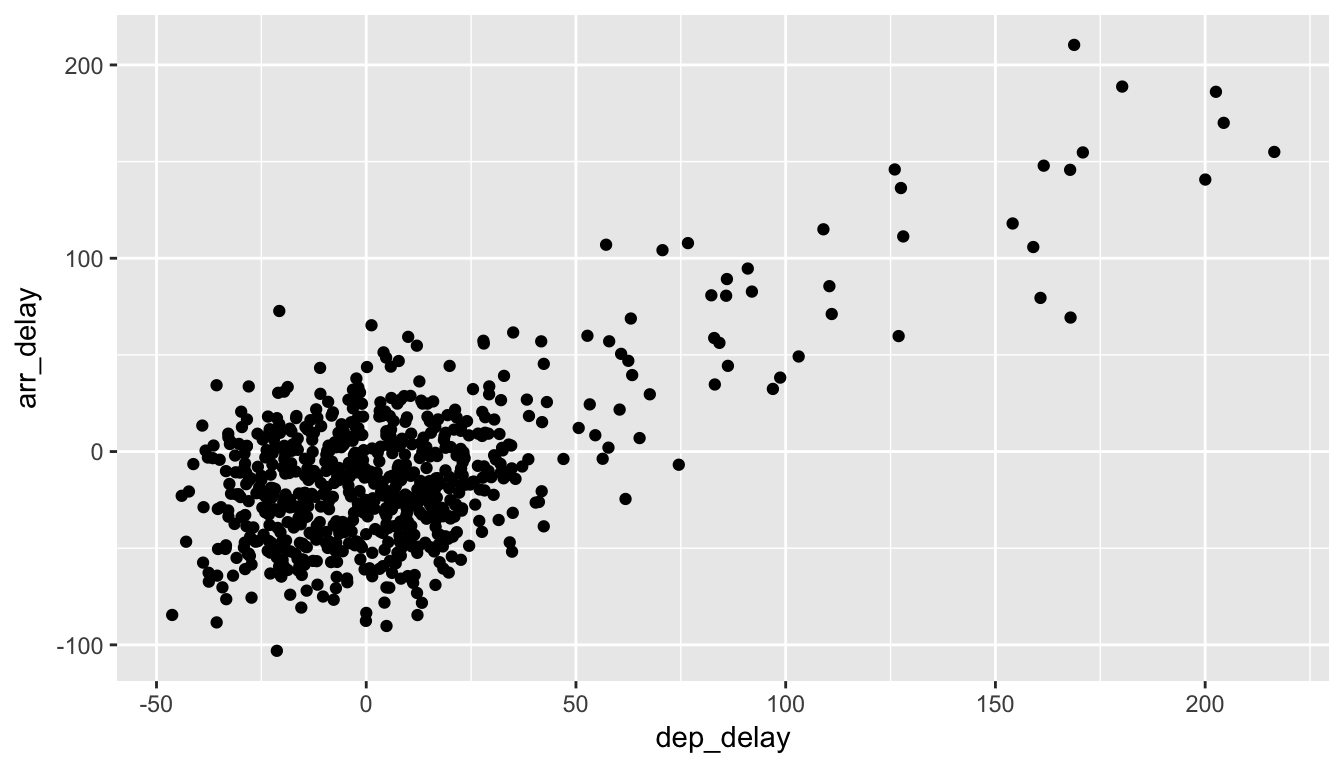
\includegraphics[width=\textwidth]{ismaykim_files/figure-latex/jitter-1} 

}

\caption[Jittered delay scatterplot]{Jittered delay scatterplot}\label{fig:jitter}
\end{figure}

Note how this function call is identical to the one in Section
\ref{geompoint}, but with \texttt{geom\_point()} replaced with
\texttt{geom\_jitter()}. The plot in \ref{fig:jitter} helps us a little
bit in getting a sense for the over-plotting, but with a relatively
large dataset like this one (714 flights), it can be argued that
changing the transparency of the points by setting \texttt{alpha} proved
more effective.

\begin{center}\rule{0.5\linewidth}{\linethickness}\end{center}

\begin{learncheck}
\textbf{\emph{Learning check}}
\end{learncheck}

\textbf{(LC4.7)} Why is setting the \texttt{alpha} argument value useful
with scatter-plots? What further information does it give you that a
regular scatter-plot cannot?

\textbf{(LC4.8)} After viewing the Figure \ref{fig:alpha} above, give a
range of arrival times and departure times that occur most frequently?
How has that region changed compared to when you observed the same plot
without the \texttt{alpha\ =\ 0.2} set in Figure \ref{fig:noalpha}?

\begin{center}\rule{0.5\linewidth}{\linethickness}\end{center}

\subsection{Summary}\label{summary}

Scatter-plots display the relationship between two continuous variables
and may be the most used plot today as they can provide an immediate way
to see the trend in one variable versus another. If you try to create a
scatter-plot where either one of the two variables is not quantitative
however, you will get strange results. Be careful!

With medium to large datasets, you may need to play with either
\texttt{geom\_jitter} or the \texttt{alpha} argument in order to get a
good feel for relationships in your data. This tweaking is often a fun
part of data visualization since you'll have the chance to see different
relationships come about as you make subtle changes to your plots.

\section{5NG\#2: Line-graphs}\label{linegraphs}

The next of the 5NG is a line-graph. They are most frequently used when
the x-axis represents time and the y-axis represents some other
numerical variable; such plots are known as \textbf{time series}. Time
represents a variable that is connected together by each day following
the previous day. In other words, time has a natural ordering.
Line-graphs should be avoided when there is not a clear sequential
ordering to the explanatory variable, i.e.~the x-variable or the
\emph{predictor} variable.

Our focus turns to the \texttt{temp} variable in this \texttt{weather}
dataset. By

\begin{itemize}
\tightlist
\item
  Looking over the \texttt{weather} dataset by typing
  \texttt{View(weather)} in the console.
\item
  Running \texttt{?weather} to bring up the help file.
\end{itemize}

We can see that the \texttt{temp} variable corresponds to hourly
temperature (in Fahrenheit) recordings at weather stations near airports
in New York City. Instead of considering all hours in 2013 for all three
airports in NYC, let's focus on the hourly temperature at Newark airport
(\texttt{origin} code ``EWR'') for the first 15 days in January 2013.
The \texttt{weather} data frame in the \texttt{nycflights13} package
contains this data, but we first need to filter it to only include those
rows that correspond to Newark in the first 15 days of January.

\begin{Shaded}
\begin{Highlighting}[]
\KeywordTok{data}\NormalTok{(weather)}
\NormalTok{early_january_weather <-}\StringTok{ }\NormalTok{weather %>%}\StringTok{ }
\StringTok{  }\KeywordTok{filter}\NormalTok{(origin ==}\StringTok{ "EWR"} \NormalTok{&}\StringTok{ }\NormalTok{month ==}\StringTok{ }\DecValTok{1} \NormalTok{&}\StringTok{ }\NormalTok{day <=}\StringTok{ }\DecValTok{15}\NormalTok{)}
\end{Highlighting}
\end{Shaded}

This is similar to the previous use of the \texttt{filter} command in
Section \ref{scatterplots}, however we now use the \texttt{\&} operator.
The above selects only those rows in \texttt{weather} where
\texttt{origin\ ==\ "EWR"} \textbf{and} \texttt{month\ =\ 1}
\textbf{and} \texttt{day\ \textless{}=\ 15}.

\begin{center}\rule{0.5\linewidth}{\linethickness}\end{center}

\begin{learncheck}
\textbf{\emph{Learning check}}
\end{learncheck}

\textbf{(LC4.9)} Take a look at both the \texttt{weather} and
\texttt{early\_january\_weather} data frames by running
\texttt{View(weather)} and \texttt{View(early\_january\_weather)} in the
console. In what respect do these data frames differ?

\textbf{(LC4.10)} The weather data is recorded hourly. Why does the
\texttt{time\_hour} variable correctly identify the hour of the
measurement whereas the \texttt{hour} variable does not?

\begin{center}\rule{0.5\linewidth}{\linethickness}\end{center}

\subsection{\texorpdfstring{Line-graphs via
\texttt{geom\_line}}{Line-graphs via geom\_line}}\label{line-graphs-via-geom_line}

We plot a line-graph of hourly temperature using \texttt{geom\_line()}:

\begin{Shaded}
\begin{Highlighting}[]
\KeywordTok{ggplot}\NormalTok{(}\DataTypeTok{data =} \NormalTok{early_january_weather, }\KeywordTok{aes}\NormalTok{(}\DataTypeTok{x =} \NormalTok{time_hour, }\DataTypeTok{y =} \NormalTok{temp)) +}
\StringTok{  }\KeywordTok{geom_line}\NormalTok{()}
\end{Highlighting}
\end{Shaded}

\begin{figure}

{\centering 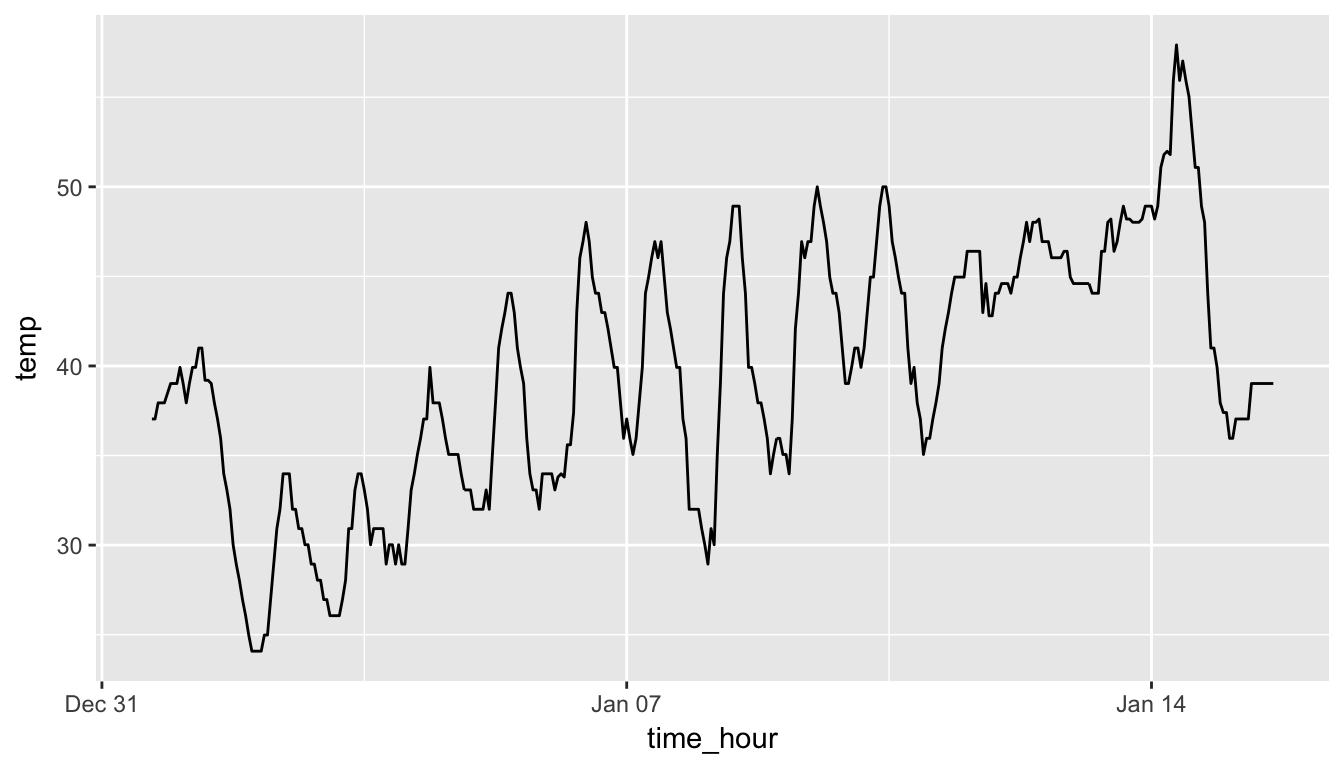
\includegraphics[width=\textwidth]{ismaykim_files/figure-latex/hourlytemp-1} 

}

\caption[Hourly Temperature in Newark for Jan 1-15 2013]{Hourly Temperature in Newark for Jan 1-15 2013}\label{fig:hourlytemp}
\end{figure}

Much as with the \texttt{ggplot()} call in Section \ref{geompoint}, we
specify the components of the Grammar of Graphics:

\begin{itemize}
\tightlist
\item
  Within the \texttt{ggplot()} function call, we specify two of the
  components of the grammar:

  \begin{enumerate}
  \def\labelenumi{\arabic{enumi}.}
  \tightlist
  \item
    The \texttt{data} frame to be \texttt{early\_january\_weather} by
    setting \texttt{data\ =\ early\_january\_weather}
  \item
    The \texttt{aes}thetic mapping by setting
    \texttt{aes(x\ =\ time\_hour,\ y\ =\ temp)}. Specifically

    \begin{itemize}
    \tightlist
    \item
      \texttt{time\_hour} (i.e.~the time variable) maps to the
      \texttt{x} position
    \item
      \texttt{temp} maps to the \texttt{y} position
    \end{itemize}
  \end{enumerate}
\item
  We add a \textbf{layer} to the \texttt{ggplot()} function call using
  the \texttt{+} sign
\item
  The layer in question specifies the third component of the grammar:
  the \texttt{geom}etric object in question. In this case the geometric
  object is a \texttt{line}, set by specifying \texttt{geom\_line()}
\end{itemize}

\begin{center}\rule{0.5\linewidth}{\linethickness}\end{center}

\begin{learncheck}
\textbf{\emph{Learning check}}
\end{learncheck}

\textbf{(LC4.11)} Why should line-graphs be avoided when there is not a
clear ordering of the horizontal axis?

\textbf{(LC4.12)} Why are line-graphs frequently used when time is the
explanatory variable?

\textbf{(LC4.13)} Plot a time series of a variable other than
\texttt{temp} for Newark Airport in the first 15 days of January 2013.

\begin{center}\rule{0.5\linewidth}{\linethickness}\end{center}

\subsection{Summary}\label{summary-1}

Line-graphs, just like scatter-plots, display the relationship between
two continuous variables. However the variable on the x-axis (i.e.~the
explanatory variable) should have a natural ordering, like some notion
of time. We can mislead our audience if that isn't the case.

\section{5NG\#3: Histograms}\label{histograms}

Let's consider the \texttt{temp} variable in the \texttt{weather} data
frame once again, but now unlike with the line-graphs in Section
\ref{linegraphs}, let's say we don't care about the relationship of
temperature to time, but rather you care about the \textbf{(statistical)
distribution} of temperatures. We could just produce points where each
of the different values appear on something similar to a number line:

\begin{figure}

{\centering 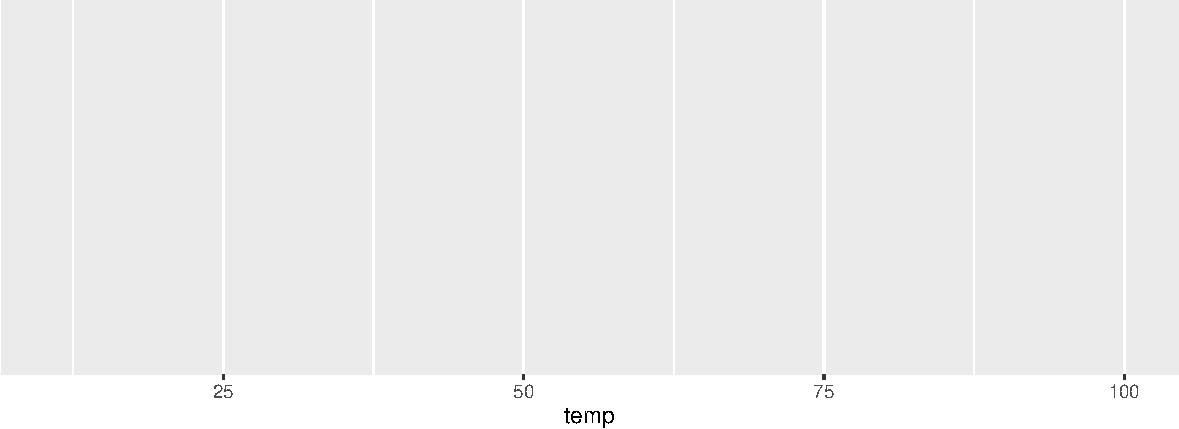
\includegraphics[width=\textwidth]{ismaykim_files/figure-latex/unnamed-chunk-15-1} 

}

\caption[Strip Plot of Hourly Temperature Recordings from NYC in 2013]{Strip Plot of Hourly Temperature Recordings from NYC in 2013}\label{fig:unnamed-chunk-15}
\end{figure}

This gives us a general idea of how the values of \texttt{temp} differ.
We see that temperatures vary from around 11 up to 100 degrees
Fahrenheit. The area between 40 and 60 degrees appears to have more
points plotted than outside that range.

\subsection{Histograms via geom\_histogram}\label{geomhistogram}

What is commonly produced instead of this strip plot is a plot known as
a \textbf{histogram}. The \textbf{histogram} shows how many elements of
a single numerical variable fall in specified \textbf{bins}. In this
case, these \textbf{bins} may correspond to between 0-10°F, 10-20°F,
etc. We produce a histogram of the hour temperatures at all three NYC
airports in 2013:

\begin{Shaded}
\begin{Highlighting}[]
\KeywordTok{ggplot}\NormalTok{(}\DataTypeTok{data =} \NormalTok{weather, }\DataTypeTok{mapping =} \KeywordTok{aes}\NormalTok{(}\DataTypeTok{x =} \NormalTok{temp)) +}
\StringTok{  }\KeywordTok{geom_histogram}\NormalTok{()}
\end{Highlighting}
\end{Shaded}

\begin{verbatim}
## `stat_bin()` using `bins = 30`. Pick better value with `binwidth`.
\end{verbatim}

\begin{verbatim}
## Warning: Removed 1 rows containing non-finite values (stat_bin).
\end{verbatim}

\begin{figure}

{\centering 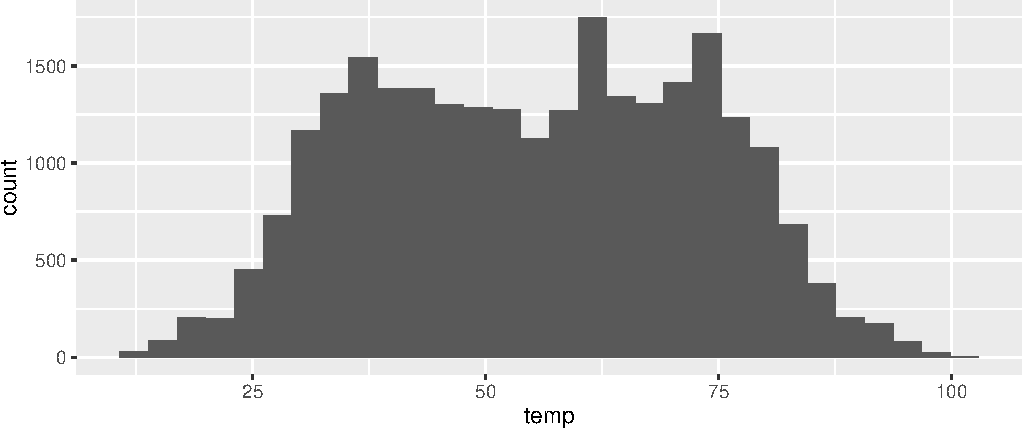
\includegraphics[width=\textwidth]{ismaykim_files/figure-latex/unnamed-chunk-16-1} 

}

\caption[Histogram of Hourly Temperature Recordings from NYC in 2013]{Histogram of Hourly Temperature Recordings from NYC in 2013}\label{fig:unnamed-chunk-16}
\end{figure}

Note here:

\begin{itemize}
\tightlist
\item
  There is only one variable being mapped in \texttt{aes()}: the single
  continuous variable \texttt{temp}. You don't need to compute the
  y-aesthetic: it gets computed automatically.
\item
  We set the \texttt{geom}etric object to be \texttt{geom\_histogram()}
\item
  We got a warning message of
  \texttt{1\ rows\ containing\ non-finite\ values} being removed. This
  is due to one of the values of temperature being missing. R is
  alerting us that this happened.
\end{itemize}

\subsection{Adjusting the Bins}\label{adjustbins}

We can adjust the number/size of the bins two ways:

\begin{enumerate}
\def\labelenumi{\arabic{enumi}.}
\tightlist
\item
  By adjusting the number of bins via the \texttt{bins} argument
\item
  By adjusting the width of the bins via the \texttt{binwidth} argument
\end{enumerate}

First, we have the power to specify how many bins we would like to put
the data into as an argument in the \texttt{geom\_histogram} function.
By default, this is chosen to be 30 somewhat arbitrarily; we have
received a warning above our plot that this was done.

\begin{Shaded}
\begin{Highlighting}[]
\KeywordTok{ggplot}\NormalTok{(}\DataTypeTok{data =} \NormalTok{weather, }\DataTypeTok{mapping =} \KeywordTok{aes}\NormalTok{(}\DataTypeTok{x =} \NormalTok{temp)) +}
\StringTok{  }\KeywordTok{geom_histogram}\NormalTok{(}\DataTypeTok{bins =} \DecValTok{60}\NormalTok{, }\DataTypeTok{color =} \StringTok{"white"}\NormalTok{)}
\end{Highlighting}
\end{Shaded}

\begin{figure}

{\centering 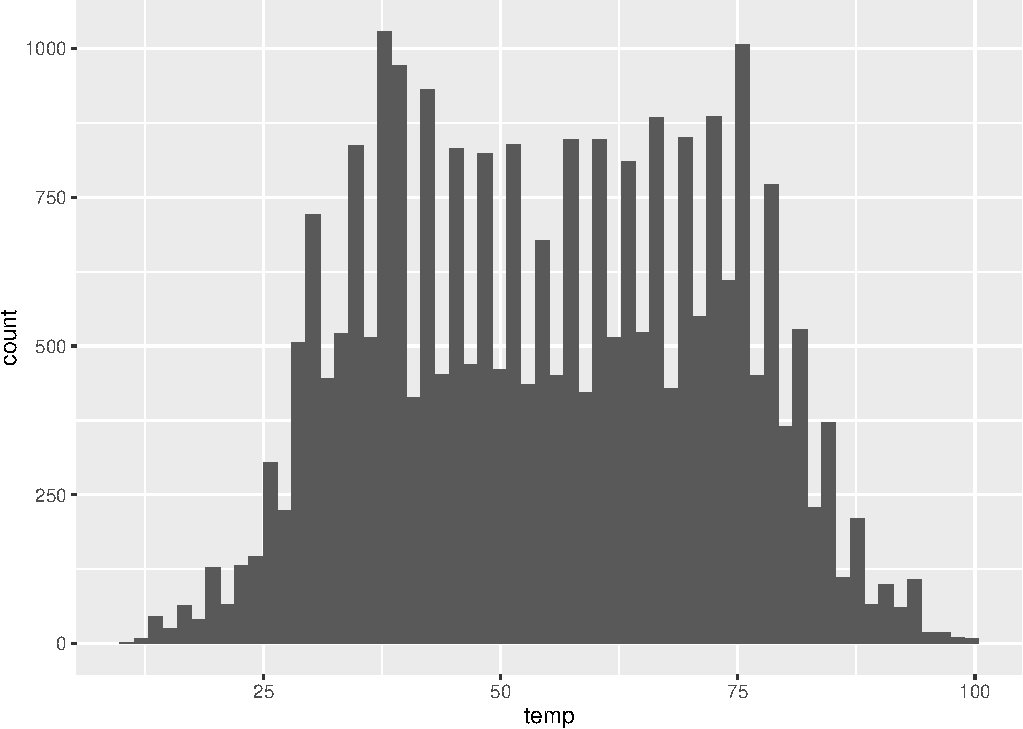
\includegraphics[width=\textwidth]{ismaykim_files/figure-latex/unnamed-chunk-17-1} 

}

\caption[Histogram of Hourly Temperature Recordings from NYC in 2013 - 60 Bins]{Histogram of Hourly Temperature Recordings from NYC in 2013 - 60 Bins}\label{fig:unnamed-chunk-17}
\end{figure}

Note the addition of the \texttt{color} argument. If you'd like to be
able to more easily differentiate each of the bins, you can specify the
color of the outline as done above.

Second, instead of specifying the number of bins, we can also specify
the width of the bins by using the \texttt{binwidth} argument in the
\texttt{geom\_histogram} function.

\begin{Shaded}
\begin{Highlighting}[]
\KeywordTok{ggplot}\NormalTok{(}\DataTypeTok{data =} \NormalTok{weather, }\DataTypeTok{mapping =} \KeywordTok{aes}\NormalTok{(}\DataTypeTok{x =} \NormalTok{temp)) +}
\StringTok{  }\KeywordTok{geom_histogram}\NormalTok{(}\DataTypeTok{binwidth =} \DecValTok{10}\NormalTok{, }\DataTypeTok{color =} \StringTok{"white"}\NormalTok{)}
\end{Highlighting}
\end{Shaded}

\begin{figure}

{\centering 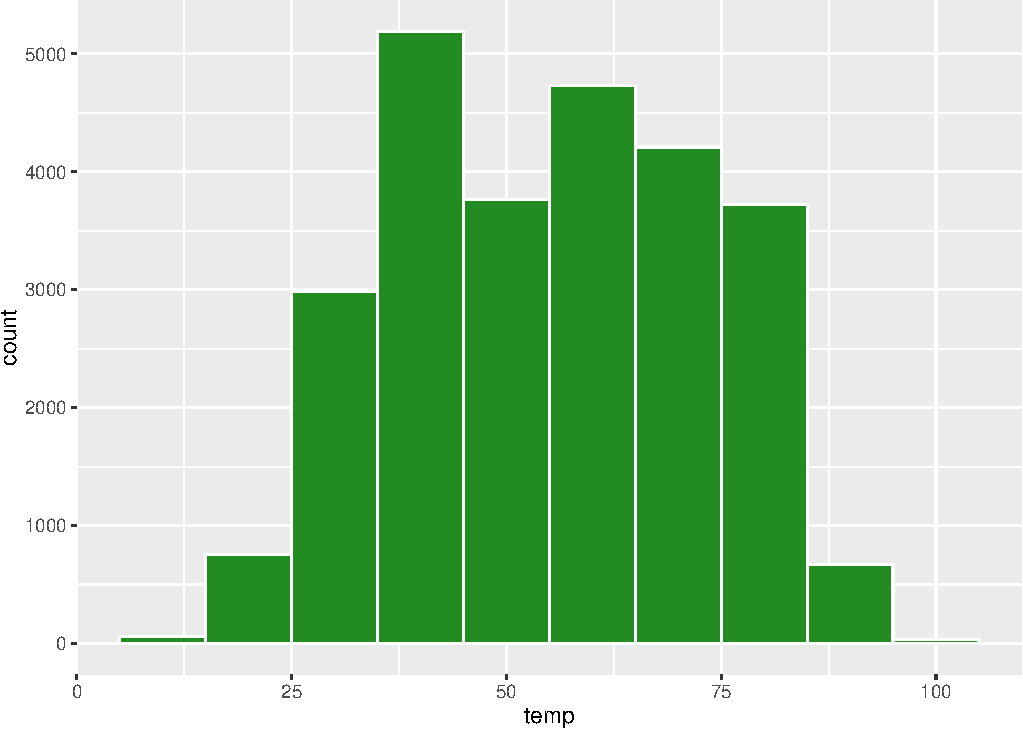
\includegraphics[width=\textwidth]{ismaykim_files/figure-latex/unnamed-chunk-18-1} 

}

\caption[Histogram of Hourly Temperature Recordings from NYC in 2013 - Binwidth = 10]{Histogram of Hourly Temperature Recordings from NYC in 2013 - Binwidth = 10}\label{fig:unnamed-chunk-18}
\end{figure}

\begin{center}\rule{0.5\linewidth}{\linethickness}\end{center}

\begin{learncheck}
\textbf{\emph{Learning check}}
\end{learncheck}

\textbf{(LC4.14)} What does changing the number of bins from 30 to 60
tell us about the distribution of temperatures?

\textbf{(LC4.15)} Would you classify the distribution of temperatures as
symmetric or skewed?

\textbf{(LC4.16)} What would you guess is the ``center'' value in this
distribution? Why did you make that choice?

\textbf{(LC4.17)} Is this data spread out greatly from the center or is
it close? Why?

\begin{center}\rule{0.5\linewidth}{\linethickness}\end{center}

\subsection{Summary}\label{summary-2}

Histograms, unlike scatter-plots and line-graphs, presents information
on only a single continuous variable. In particular they are
visualizations of the (statistical) distribution of values.

\section{Facets}\label{facets}

Before continuing the 5NG, we briefly introduce a new concept called
\textbf{faceting}. Faceting is used when we'd like to create small
multiples of the same plot over a different categorical variable. By
default, all of the small multiples will have the same vertical axis.

For example, suppose we were interested in looking at how the
temperature histograms we saw in Section \ref{histograms} varied by
month. This is what is meant by ``the distribution of a variable over
another variable'': \texttt{temp} is one variable and \texttt{month} is
the other variable. In order to look at histograms of \texttt{temp} for
each month, we add a layer \texttt{facet\_wrap(\textasciitilde{}month)}.
You can also specify how many rows you'd like the small multiple plots
to be in using \texttt{nrow} inside of \texttt{facet\_wrap}.

\begin{Shaded}
\begin{Highlighting}[]
\KeywordTok{ggplot}\NormalTok{(}\DataTypeTok{data =} \NormalTok{weather, }\KeywordTok{aes}\NormalTok{(}\DataTypeTok{x =} \NormalTok{temp)) +}
\StringTok{  }\KeywordTok{geom_histogram}\NormalTok{(}\DataTypeTok{binwidth =} \DecValTok{5}\NormalTok{, }\DataTypeTok{color =} \StringTok{"white"}\NormalTok{) +}
\StringTok{  }\KeywordTok{facet_wrap}\NormalTok{(~}\StringTok{ }\NormalTok{month, }\DataTypeTok{nrow =} \DecValTok{4}\NormalTok{)}
\end{Highlighting}
\end{Shaded}

\begin{figure}

{\centering 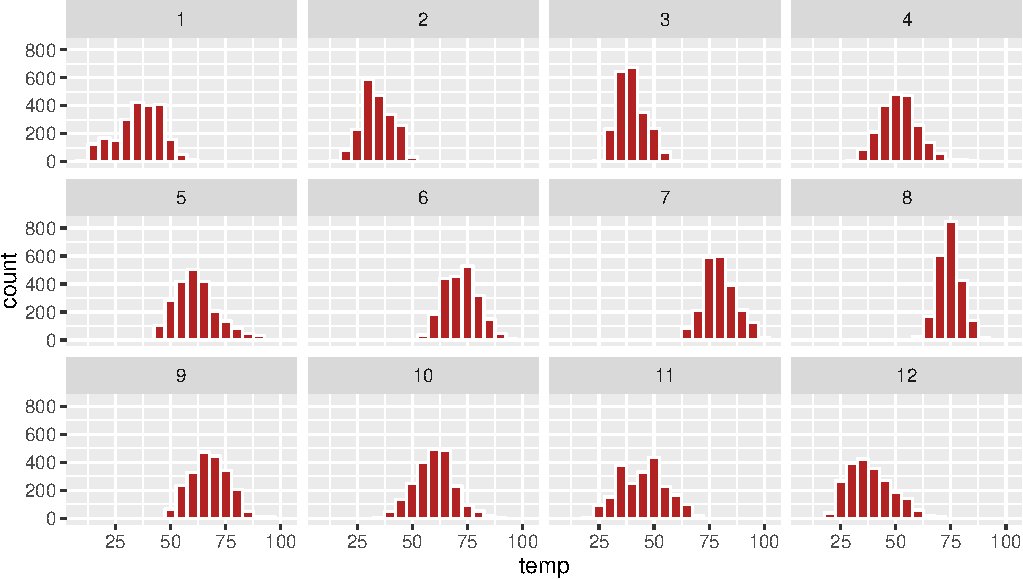
\includegraphics[width=\textwidth]{ismaykim_files/figure-latex/facethistogram-1} 

}

\caption[Faceted histogram]{Faceted histogram}\label{fig:facethistogram}
\end{figure}

As we might expect, the temperature tends to increase as summer
approaches and then decrease as winter approaches.

\begin{center}\rule{0.5\linewidth}{\linethickness}\end{center}

\begin{learncheck}
\textbf{\emph{Learning check}}
\end{learncheck}

\textbf{(LC4.18)} What other things do you notice about the faceted plot
above? How does a faceted plot help us see how relationships between two
variables?

\textbf{(LC4.19)} What do the numbers 1-12 correspond to in the plot
above? What about 25, 50, 75, 100?

\textbf{(LC4.20)} For which types of datasets would these types of
faceted plots not work well in comparing relationships between
variables? Give an example describing the variability of the variables
and other important characteristics.

\textbf{(LC4.21)} Does the \texttt{temp} variable in the
\texttt{weather} data set have a lot of variability? Why do you say
that?

\begin{center}\rule{0.5\linewidth}{\linethickness}\end{center}

\section{5NG\#4: Boxplots}\label{ng4-boxplots}

While using faceted histograms can provide a way to compare
distributions of a continuous variable split by groups of a categorical
variable as in Chapter \ref{facets}, an alternative plot called a
\textbf{boxplot} (also called a \textbf{side-by-side boxplot}) achieves
the same task and is frequently preferred. The \textbf{boxplot} uses the
information provided in the \textbf{five-number summary} referred to in
Appendix \ref{appendixA}. It gives a way to compare this summary
information across the different levels of a categorical variable.

\subsection{\texorpdfstring{Boxplots via
\texttt{geom\_boxplot}}{Boxplots via geom\_boxplot}}\label{boxplots-via-geom_boxplot}

Let's create a boxplot to compare the monthly temperatures as we did
above with the faceted histograms.

\begin{Shaded}
\begin{Highlighting}[]
\KeywordTok{ggplot}\NormalTok{(}\DataTypeTok{data =} \NormalTok{weather, }\KeywordTok{aes}\NormalTok{(}\DataTypeTok{x =} \NormalTok{month, }\DataTypeTok{y =} \NormalTok{temp)) +}
\StringTok{  }\KeywordTok{geom_boxplot}\NormalTok{()}
\end{Highlighting}
\end{Shaded}

\begin{figure}

{\centering 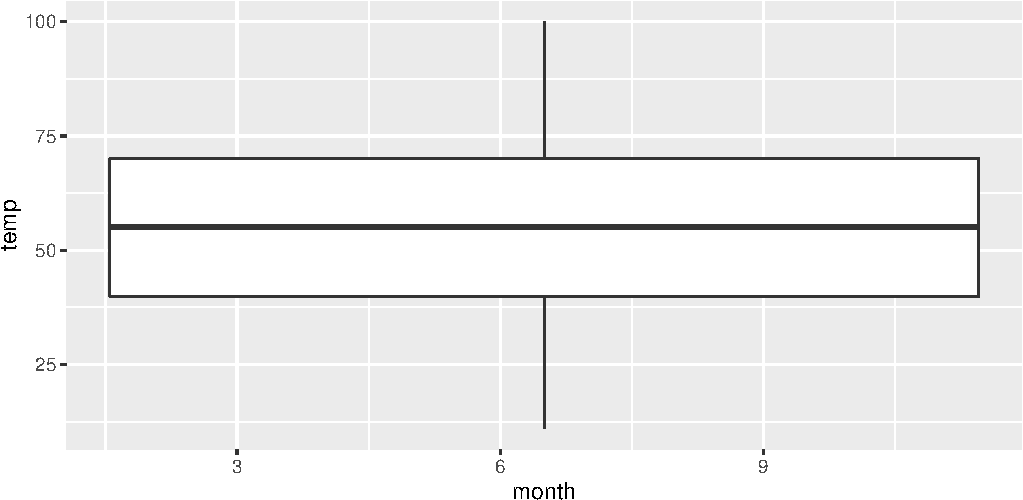
\includegraphics[width=\textwidth]{ismaykim_files/figure-latex/badbox-1} 

}

\caption[Invalid boxplot specification]{Invalid boxplot specification}\label{fig:badbox}
\end{figure}

Note the first warning that is given here. (The second one corresponds
to missing values in the data frame and it is turned off on subsequent
plots.) Observe that this plot does not look like what we were
expecting. We were expecting to see the distribution of temperatures for
each month (so 12 different boxplots). This gives us the overall boxplot
without any other groupings. We can get around this by introducing a new
function for our \texttt{x} variable:

\begin{Shaded}
\begin{Highlighting}[]
\KeywordTok{ggplot}\NormalTok{(}\DataTypeTok{data =} \NormalTok{weather, }\DataTypeTok{mapping =} \KeywordTok{aes}\NormalTok{(}\DataTypeTok{x =} \KeywordTok{factor}\NormalTok{(month), }\DataTypeTok{y =} \NormalTok{temp)) +}
\StringTok{  }\KeywordTok{geom_boxplot}\NormalTok{()}
\end{Highlighting}
\end{Shaded}

\begin{figure}

{\centering 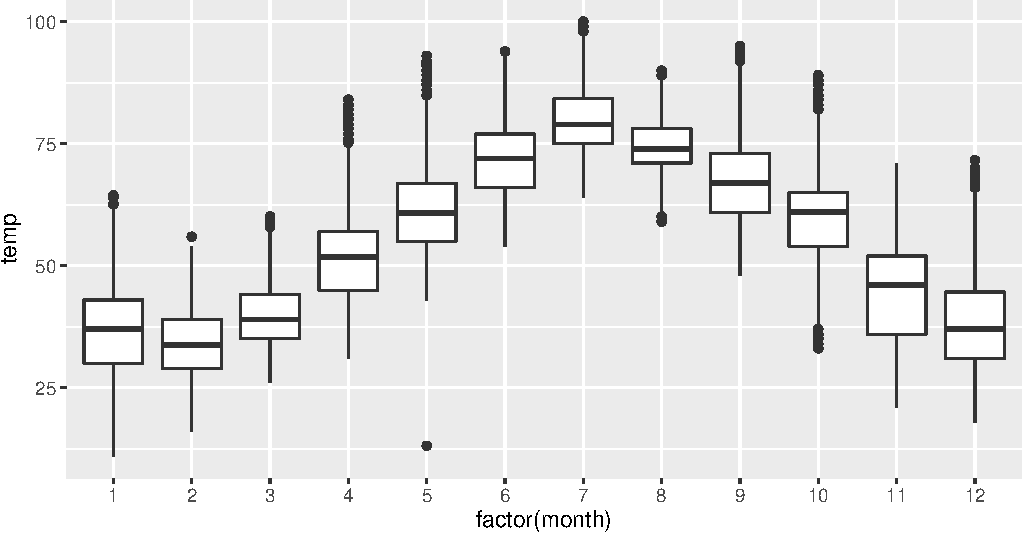
\includegraphics[width=\textwidth]{ismaykim_files/figure-latex/monthtempbox-1} 

}

\caption[Month by temp boxplot]{Month by temp boxplot}\label{fig:monthtempbox}
\end{figure}

We have introduced a new function called \texttt{factor()} here. One of
the things this function does is to convert a discrete value like
\texttt{month} (1, 2, \ldots{}, 12) into a categorical variable. The
``box'' part of this plot represents the 25\textsuperscript{th}
percentile, the median (50\textsuperscript{th} percentile), and the
75\textsuperscript{th} percentile. The dots correspond to
\textbf{outliers}. (The specific formulation for these outliers is
discussed in Appendix \ref{appendixA}.) The lines show how the data
varies that is not in the center 50\% defined by the first and third
quantiles. Longer lines correspond to more variability and shorter lines
correspond to less variability.

\begin{center}\rule{0.5\linewidth}{\linethickness}\end{center}

\begin{learncheck}
\textbf{\emph{Learning check}}
\end{learncheck}

\textbf{(LC4.22)} What does the dot at the bottom of the plot for May
correspond to? Explain what might have occurred in May to produce this
point.

\textbf{(LC4.23)} Which months have the highest variability in
temperature? What reasons do you think this is?

\textbf{(LC4.24)} We looked at the distribution of a continuous variable
over a categorical variable here with this boxplot. Why can't we look at
the distribution of one continuous variable over the distribution of
another continuous variable? Say, temperature across pressure, for
example?

\textbf{(LC4.25)} Boxplots provide a simple way to identify outliers.
Why may outliers be easier to identify when looking at a boxplot instead
of a faceted histogram?

\begin{center}\rule{0.5\linewidth}{\linethickness}\end{center}

\subsection{Summary}\label{summary-3}

Boxplots provide a way to compare and contrast the distribution of one
quantitative variable across multiple levels of one categorical
variable. One can easily look to see where the median falls across the
different groups by looking at the center line in the box. You can also
see how spread out the variable is across the different groups by
looking at the width of the box and also how far out the lines stretch
from the box. If the lines stretch far from the box but the box has a
small width, the variability of the values closer to the center is much
smaller than the variability of the outer ends of the variable. Lastly,
outliers are even more easily identified when looking at a boxplot than
when looking at a histogram.

\section{5NG\#5: Barplots}\label{geombar}

Both histograms and boxplots represent ways to visualize the variability
of continuous variables. Another common task is to present the
distribution of a categorical variable. This is a simpler task since we
will be interested in how many elements from our data fall into the
different categories of the categorical variable.

\subsection{\texorpdfstring{Barplots via
\texttt{geom\_bar}}{Barplots via geom\_bar}}\label{barplots-via-geom_bar}

Frequently, the best way to visualize these different counts (also known
as \textbf{frequencies}) is via a barplot. Consider the distribution of
airlines that flew out of New York City in 2013. Here we explore the
number of flights from each airline/\texttt{carrier}. This can be
plotted by invoking the \texttt{geom\_bar} function in \texttt{ggplot2}:

\begin{Shaded}
\begin{Highlighting}[]
\KeywordTok{ggplot}\NormalTok{(}\DataTypeTok{data =} \NormalTok{flights, }\DataTypeTok{mapping =} \KeywordTok{aes}\NormalTok{(}\DataTypeTok{x =} \NormalTok{carrier)) +}
\StringTok{  }\KeywordTok{geom_bar}\NormalTok{()}
\end{Highlighting}
\end{Shaded}

\begin{figure}

{\centering 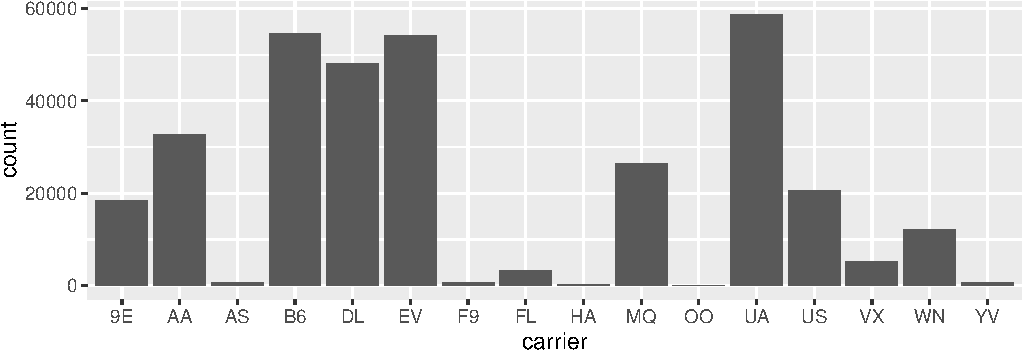
\includegraphics[width=\textwidth]{ismaykim_files/figure-latex/flightsbar-1} 

}

\caption[Number of flights departing NYC in 2013 by airline]{Number of flights departing NYC in 2013 by airline}\label{fig:flightsbar}
\end{figure}

To get an understanding of what the names of these airlines are
corresponding to these \texttt{carrier} codes, we can look at the
\texttt{airlines} data frame in the \texttt{nycflights13} package. Note
the use of the \texttt{kable} function here in the \texttt{knitr}
package, which produces a nicely-formatted table of the values in the
\texttt{airlines} data frame.

\begin{Shaded}
\begin{Highlighting}[]
\KeywordTok{data}\NormalTok{(airlines)}
\KeywordTok{kable}\NormalTok{(airlines)}
\end{Highlighting}
\end{Shaded}

\begin{tabular}{l|l}
\hline
carrier & name\\
\hline
9E & Endeavor Air Inc.\\
\hline
AA & American Airlines Inc.\\
\hline
AS & Alaska Airlines Inc.\\
\hline
B6 & JetBlue Airways\\
\hline
DL & Delta Air Lines Inc.\\
\hline
EV & ExpressJet Airlines Inc.\\
\hline
F9 & Frontier Airlines Inc.\\
\hline
FL & AirTran Airways Corporation\\
\hline
HA & Hawaiian Airlines Inc.\\
\hline
MQ & Envoy Air\\
\hline
OO & SkyWest Airlines Inc.\\
\hline
UA & United Air Lines Inc.\\
\hline
US & US Airways Inc.\\
\hline
VX & Virgin America\\
\hline
WN & Southwest Airlines Co.\\
\hline
YV & Mesa Airlines Inc.\\
\hline
\end{tabular}

Going back to our barplot, we see that United Air Lines, JetBlue
Airways, and ExpressJet Airlines had the most flights depart New York
City in 2013. To get the actual number of flights by each airline we can
use the \texttt{count} function in the \texttt{dplyr} package on the
\texttt{carrier} variable in \texttt{flights}, which we will introduce
formally in Chapter \ref{manip}.

\begin{Shaded}
\begin{Highlighting}[]
\NormalTok{flights_table <-}\StringTok{ }\NormalTok{flights %>%}\StringTok{ }\NormalTok{dplyr::}\KeywordTok{count}\NormalTok{(carrier)}
\NormalTok{knitr::}\KeywordTok{kable}\NormalTok{(flights_table)}
\end{Highlighting}
\end{Shaded}

\begin{tabular}{l|r}
\hline
carrier & n\\
\hline
9E & 18460\\
\hline
AA & 32729\\
\hline
AS & 714\\
\hline
B6 & 54635\\
\hline
DL & 48110\\
\hline
EV & 54173\\
\hline
F9 & 685\\
\hline
FL & 3260\\
\hline
HA & 342\\
\hline
MQ & 26397\\
\hline
OO & 32\\
\hline
UA & 58665\\
\hline
US & 20536\\
\hline
VX & 5162\\
\hline
WN & 12275\\
\hline
YV & 601\\
\hline
\end{tabular}

\textbf{Technical note}: Refer to the use of \texttt{::} in both lines
of code above. This is another way of ensuring the correct function is
called. A \texttt{count} exists in a couple different packages and
sometimes you'll receive strange errors when a different instance of a
function is used. This is a great way of telling R that ``I want this
one!''. You specify the name of the package directly before the
\texttt{::} and then the name of the function immediately after
\texttt{::}.

\begin{center}\rule{0.5\linewidth}{\linethickness}\end{center}

\begin{learncheck}
\textbf{\emph{Learning check}}
\end{learncheck}

\textbf{(LC4.26)} Why are histograms inappropriate for visualizing
categorical variables?

\textbf{(LC4.27)} What is the difference between histograms and
barplots?

\textbf{(LC4.28)} How many Envoy Air flights departed NYC in 2013?

\textbf{(LC4.29)} What was the seventh highest airline in terms of
departed flights from NYC in 2013? How could we better present the table
to get this answer quickly.

\begin{center}\rule{0.5\linewidth}{\linethickness}\end{center}

\subsection{Must avoid pie charts!}\label{must-avoid-pie-charts}

Unfortunately, one of the most common plots seen today for categorical
data is the pie chart. While they may see harmless enough, they actually
present a problem in that humans are unable to judge angles well. As
Naomi Robbins describes in her book ``Creating More Effective Graphs''
\citep{robbins2013}, we overestimate angles greater than 90 degrees and
we underestimate angles less than 90 degrees. In other words, it is
difficult for us to determine relative size of one piece of the pie
compared to another.

Let's examine our previous barplot example on the number of flights
departing NYC by airline. This time we will use a pie chart. As you
review this chart, try to identify

\begin{itemize}
\tightlist
\item
  how much larger the portion of the pie is for ExpressJet Airlines
  (\texttt{EV}) compared to US Airways (\texttt{US}),
\item
  what the third largest carrier is in terms of departing flights, and
\item
  how many carriers have fewer flights than United Airlines
  (\texttt{UA})?
\end{itemize}

\begin{figure}

{\centering 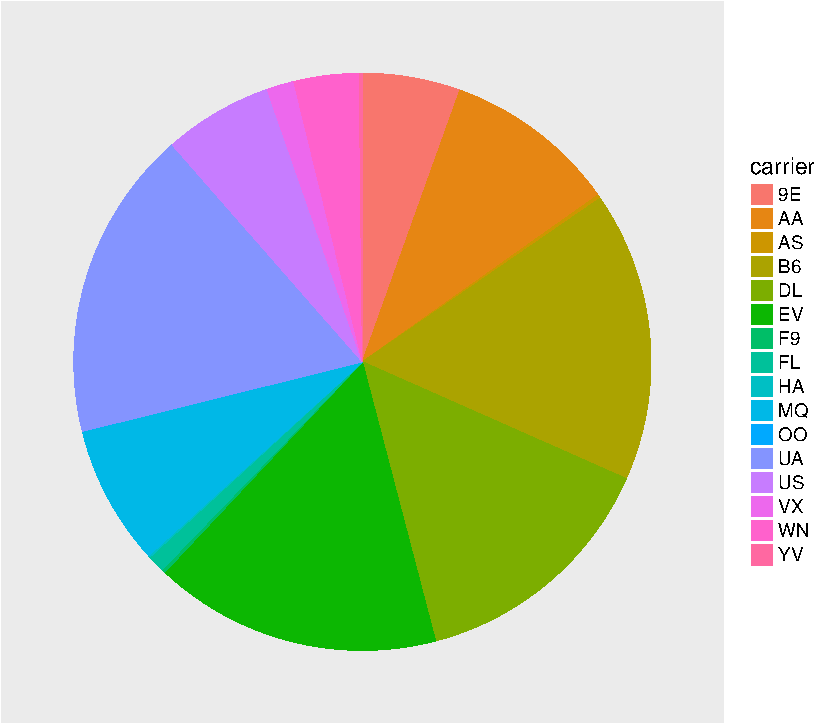
\includegraphics[width=\textwidth]{ismaykim_files/figure-latex/carrierpie-1} 

}

\caption[The dreaded pie chart]{The dreaded pie chart}\label{fig:carrierpie}
\end{figure}

While it is quite easy to look back at the barplot to get the answer to
these questions, it's quite difficult to get the answers correct when
looking at the pie graph. Barplots can always present the information in
a way that is easier for the eye to determine relative position. There
may be one exception from Nathan Yau at
\href{https://flowingdata.com/2008/09/19/pie-i-have-eaten-and-pie-i-have-not-eaten/}{FlowingData.com}
but we will leave this for the reader to decide:

\begin{figure}

{\centering 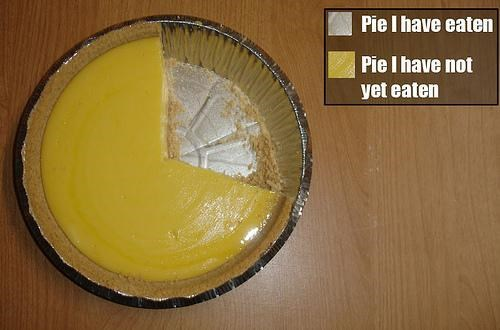
\includegraphics[width=\textwidth,height=2.5in]{images/Pie-I-have-Eaten} 

}

\caption[The only good pie chart]{The only good pie chart}\label{fig:unnamed-chunk-21}
\end{figure}

\begin{center}\rule{0.5\linewidth}{\linethickness}\end{center}

\begin{learncheck}
\textbf{\emph{Learning check}}
\end{learncheck}

\textbf{(LC4.30)} Why should pie charts be avoided and replaced by
barplots?

\textbf{(LC4.31)} What is your opinion as to why pie charts continue to
be used?

\begin{center}\rule{0.5\linewidth}{\linethickness}\end{center}

\subsection{Using barplots to compare two
variables}\label{using-barplots-to-compare-two-variables}

Barplots are the go-to way to visualize the frequency of different
categories of a categorical variable. They make it easy to order the
counts and to compare one group's frequency to another. Another use of
barplots (unfortunately, sometimes inappropriately and confusingly) is
to compare two categorical variables together. Let's examine the
distribution of outgoing flights from NYC by \texttt{carrier} and
\texttt{airport}.

We begin by getting the names of the airports in NYC that were included
in the \texttt{flights} dataset. Remember from Chapter \ref{tidy} that
this can be done by using the \texttt{inner\_join} function (more in
Chapter \ref{manip}).

\begin{Shaded}
\begin{Highlighting}[]
\NormalTok{flights_namedports <-}\StringTok{ }\NormalTok{flights %>%}\StringTok{ }
\StringTok{  }\KeywordTok{inner_join}\NormalTok{(airports, }\DataTypeTok{by =} \KeywordTok{c}\NormalTok{(}\StringTok{"origin"} \NormalTok{=}\StringTok{ "faa"}\NormalTok{))}
\end{Highlighting}
\end{Shaded}

After running \texttt{View(flights\_namedports)}, we see that
\texttt{name} now corresponds to the name of the airport as referenced
by the \texttt{origin} variable. We will now plot \texttt{carrier} as
the horizontal variable. When we specify \texttt{geom\_bar}, it will
specify \texttt{count} as being the vertical variable. A new addition
here is \texttt{fill\ =\ name}. Look over what was produced from the
plot to get an idea of what this argument gives.

Note that \texttt{fill} is an \texttt{aes}thetic just like \texttt{x} is
an \texttt{aes}thetic. We need to make the \texttt{name} variable to
this \texttt{aes}thetic. Any time you use a variable like this, you need
to make sure it is wrapped inside the \texttt{aes} function.
\textbf{This is a common error!} Make note of this now so you don't fall
into this problem later.

\begin{Shaded}
\begin{Highlighting}[]
\KeywordTok{ggplot}\NormalTok{(}\DataTypeTok{data =} \NormalTok{flights_namedports, }\DataTypeTok{mapping =} \KeywordTok{aes}\NormalTok{(}\DataTypeTok{x =} \NormalTok{carrier, }\DataTypeTok{fill =} \NormalTok{name)) +}
\StringTok{  }\KeywordTok{geom_bar}\NormalTok{()}
\end{Highlighting}
\end{Shaded}

\begin{figure}

{\centering 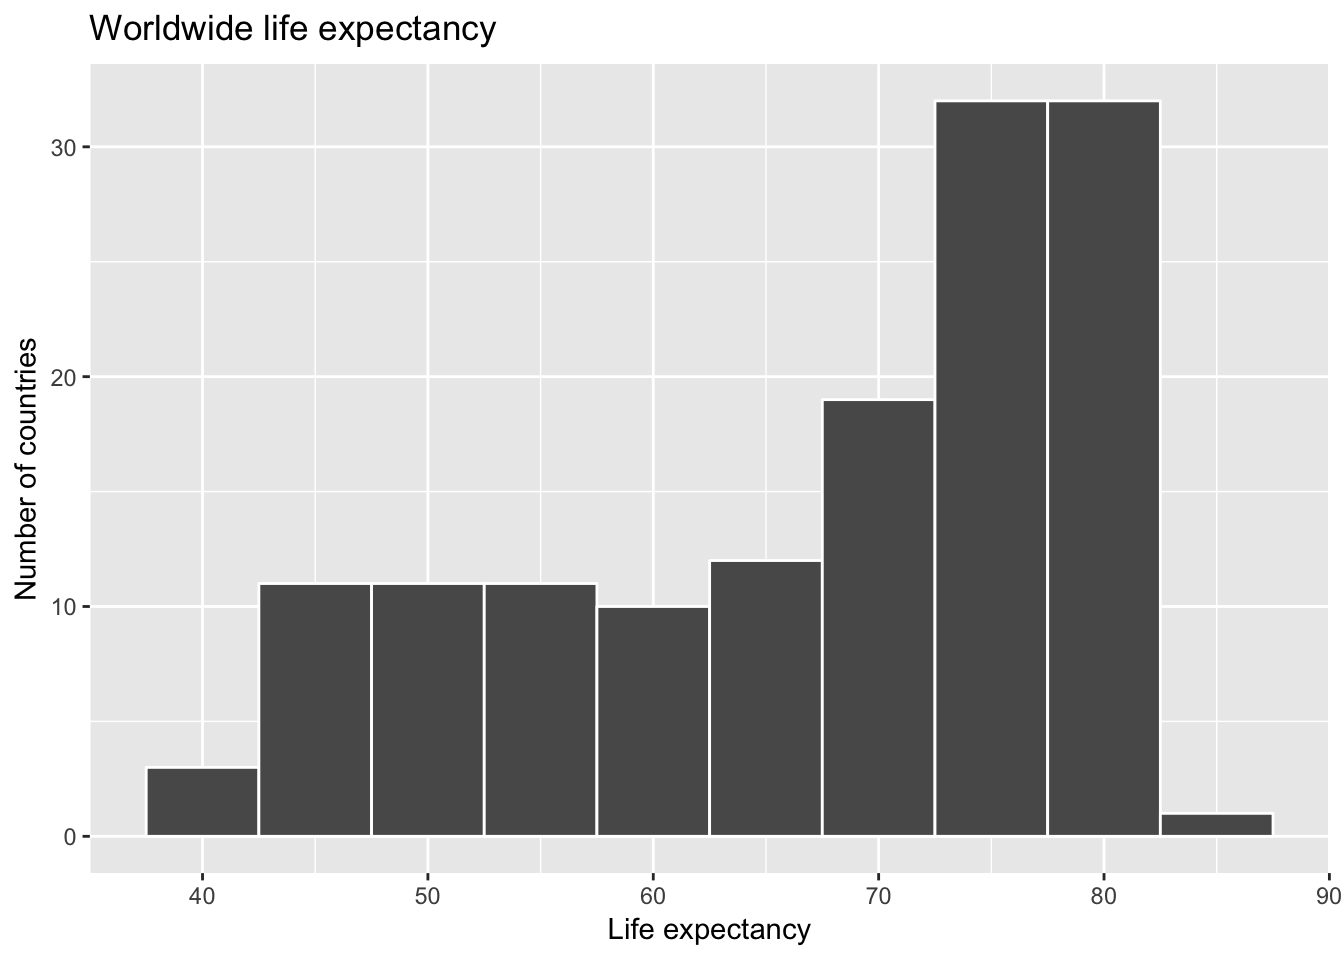
\includegraphics[width=\textwidth]{ismaykim_files/figure-latex/unnamed-chunk-23-1} 

}

\caption[Stacked barplot comparing the number of flights by carrier and airport]{Stacked barplot comparing the number of flights by carrier and airport}\label{fig:unnamed-chunk-23}
\end{figure}

This plot is what is known as a \textbf{stacked barplot}. While simple
to make, it often leads to many problems.

\begin{center}\rule{0.5\linewidth}{\linethickness}\end{center}

\begin{learncheck}
\textbf{\emph{Learning check}}
\end{learncheck}

\textbf{(LC4.32)} What kinds of questions are not easily answered by
looking at the above figure?

\textbf{(LC4.33)} What can you say, if anything, about the relationship
between airline and airport in NYC in 2013 in regards to the number of
departing flights?

\begin{center}\rule{0.5\linewidth}{\linethickness}\end{center}

Another variation on the \textbf{stacked barplot} is the
\textbf{side-by-side barplot}.

\begin{Shaded}
\begin{Highlighting}[]
\KeywordTok{ggplot}\NormalTok{(}\DataTypeTok{data =} \NormalTok{flights_namedports, }\DataTypeTok{mapping =} \KeywordTok{aes}\NormalTok{(}\DataTypeTok{x =} \NormalTok{carrier, }\DataTypeTok{fill =} \NormalTok{name)) +}
\StringTok{  }\KeywordTok{geom_bar}\NormalTok{(}\DataTypeTok{position =} \StringTok{"dodge"}\NormalTok{)}
\end{Highlighting}
\end{Shaded}

\begin{figure}

{\centering 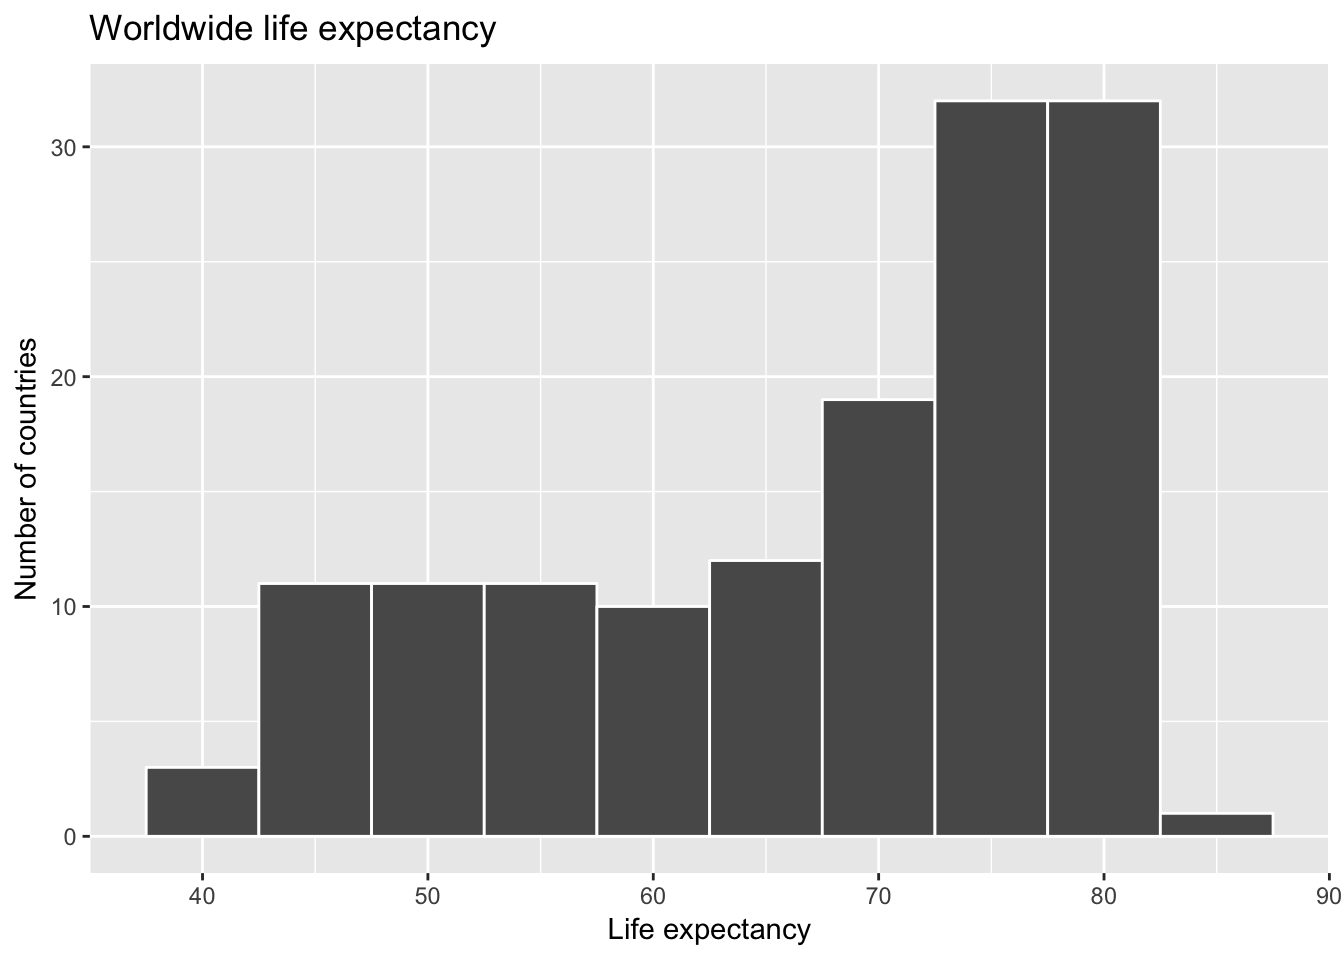
\includegraphics[width=\textwidth]{ismaykim_files/figure-latex/unnamed-chunk-24-1} 

}

\caption[Side-by-side barplot comparing the number of flights by carrier and airport]{Side-by-side barplot comparing the number of flights by carrier and airport}\label{fig:unnamed-chunk-24}
\end{figure}

\begin{center}\rule{0.5\linewidth}{\linethickness}\end{center}

\begin{learncheck}
\textbf{\emph{Learning check}}
\end{learncheck}

\textbf{(LC4.34)} Why might the side-by-side barplot be preferable to a
stacked barplot in this case?

\textbf{(LC4.35)} What are the disadvantages of using a side-by-side
barplot, in general?

\begin{center}\rule{0.5\linewidth}{\linethickness}\end{center}

Lastly, an often preferred type of barplot is the \textbf{faceted
barplot}. We already saw this concept of faceting and small multiples in
Section \ref{facets}. This gives us a nicer way to compare the
distributions across both \texttt{carrier} and airport/\texttt{name}.

\begin{Shaded}
\begin{Highlighting}[]
\KeywordTok{ggplot}\NormalTok{(}\DataTypeTok{data =} \NormalTok{flights_namedports, }\DataTypeTok{mapping =} \KeywordTok{aes}\NormalTok{(}\DataTypeTok{x =} \NormalTok{carrier, }\DataTypeTok{fill =} \NormalTok{name)) +}
\StringTok{  }\KeywordTok{geom_bar}\NormalTok{() +}
\StringTok{  }\KeywordTok{facet_grid}\NormalTok{(name ~}\StringTok{ }\NormalTok{.)}
\end{Highlighting}
\end{Shaded}

\begin{figure}

{\centering 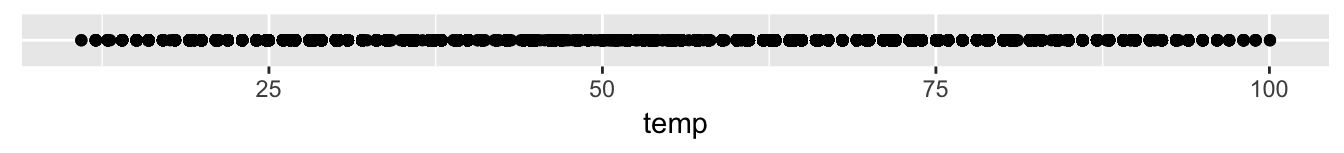
\includegraphics[width=\textwidth]{ismaykim_files/figure-latex/unnamed-chunk-25-1} 

}

\caption[Faceted barplot comparing the number of flights by carrier and airport]{Faceted barplot comparing the number of flights by carrier and airport}\label{fig:unnamed-chunk-25}
\end{figure}

Note how the \texttt{facet\_grid} function arguments are written here.
We are wanting the names of the airports vertically and the
\texttt{carrier} listed horizontally. As you may have guessed, this
argument and other \emph{formulas} of this sort in R are in
\texttt{y\ \textasciitilde{}\ x} order. We will see more examples of
this in Chapter \ref{regress}.

\begin{center}\rule{0.5\linewidth}{\linethickness}\end{center}

\begin{learncheck}
\textbf{\emph{Learning check}}
\end{learncheck}

\textbf{(LC4.36)} Why is the faceted barplot preferred to the
side-by-side and stacked barplots in this case?

\textbf{(LC4.37)} What information about the different carriers at
different airports is more easily seen in the faceted barplot?

\begin{center}\rule{0.5\linewidth}{\linethickness}\end{center}

\subsection{Summary}\label{summary-4}

Barplots are the preferred way of displaying categorical variables. They
are easy-to-understand and to make comparisons across groups of a
categorical variable. When dealing with more than one categorical
variable, faceted barplots are frequently preferred over side-by-side or
stacked barplots. Stacked barplots are sometimes nice to look at, but it
is quite difficult to compare across the levels since the sizes of the
bars are all of different sizes. Side-by-side barplots can provide an
improvement on this, but the issue about comparing across groups still
must be dealt with.

\section{Conclusion}\label{conclusion}

\subsection{Resources}\label{resources}

An excellent resource as you begin to create plots using the
\texttt{ggplot2} package is a cheatsheet that RStudio has put together
entitled ``Data Visualization with ggplot2'' available

\begin{itemize}
\tightlist
\item
  By clicking
  \href{https://www.rstudio.com/wp-content/uploads/2015/12/ggplot2-cheatsheet-2.0.pdf}{here}
\item
  or by clicking the RStudio Menu Bar -\textgreater{} Help
  -\textgreater{} Cheatsheets -\textgreater{} ``Data Visualization with
  \texttt{ggplot2}''
\end{itemize}

This covers more than what we've discussed in this chapter but provides
nice visual descriptions of what each function produces.

\subsection{Script of R code}\label{script-of-r-code}

An R script file of all R code used in this chapter is available
\href{http://ismayc.github.io/moderndiver-book/04-viz.R}{here}.

\subsection{What's to come?}\label{whats-to-come-1}

In Chapter \ref{manip}, we'll further explore data by grouping our data,
creating summaries based on those groupings, filtering our data to match
conditions, selecting specific columns of our data, and other
manipulations with our data including defining new columns/variables.
These data manipulation procedures will go hand-in-hand with the data
visualizations you've produced here.

\chapter{Data Manipulation via dplyr}\label{manip}

Let's briefly recap where we have been so far and where we are headed.
In Chapter \ref{tidy}, we discussed what it means for data to be tidy.
We saw that this refers to observational units corresponding to rows and
variables being stored in columns. The entries in the data frame
correspond to different combinations of observational units and
variables. In the \texttt{flights} data frame, we saw that each row
corresponds to a different flight leaving New York City. In other words,
the observational unit of that tidy data frame is a flight. The
variables are listed as columns and for \texttt{flights} they include
both quantitative variables like \texttt{dep\_delay} and
\texttt{distance} but also categorical variables like \texttt{carrier}
and \texttt{origin}. An entry in the table corresponds to a particular
flight on a given day and a particular value of a given variable
representing that flight.

We saw in Chapter \ref{viz} that organizing data in this tidy way makes
it easy for us to produce graphics. We can simply specify what
variable/column we would like on one axis, what variable we'd like on
the other axis, and what type of plot we'd like to make. We can also do
things such as changing the color by another variable or change the size
of our points by a fourth variable given this tidy data set.

Furthermore, in Chapter \ref{viz}, we hinted at some ways to summarize
and manipulate data to suit your needs. This chapter expands on this by
giving a variety of examples using what we call the \emph{Five Main
Verbs} in the \texttt{dplyr} package \citep{R-dplyr}. There are more
advanced operations than just these and you'll see some examples of this
near the end of the chapter.

\section*{Needed packages}\label{needed-packages-1}
\addcontentsline{toc}{section}{Needed packages}

Before we proceed with this chapter, let's load all the necessary
packages.

\begin{Shaded}
\begin{Highlighting}[]
\KeywordTok{library}\NormalTok{(dplyr)}
\KeywordTok{library}\NormalTok{(ggplot2)}
\KeywordTok{library}\NormalTok{(nycflights13)}
\KeywordTok{library}\NormalTok{(knitr)}
\end{Highlighting}
\end{Shaded}

\section{\texorpdfstring{The pipe
\texttt{\%\textgreater{}\%}}{The pipe \%\textgreater{}\%}}\label{the-pipe}

Before we introduce the five main verbs, we first introduce the the pipe
operator (\texttt{\%\textgreater{}\%}). Just as the \texttt{+} sign was
used to add layers to a plot created using \texttt{ggplot()}, the pipe
operator allows us to chain together \texttt{dplyr} data manipulation
functions. The pipe operator can be read read as ``\emph{then}''. The
\texttt{\%\textgreater{}\%} operator allows us to go from one step in
\texttt{dplyr} to the next easily so we can for example:

\begin{itemize}
\tightlist
\item
  \texttt{filter} our data frame to only focus on a few rows \emph{then}
\item
  \texttt{group\_by} another variable to create groups \emph{then}
\item
  \texttt{summarize} this grouped data to calculate the mean for each
  level of the group.
\end{itemize}

The piping syntax will be our major focus throughout the rest of this
book and you'll find that you'll quickly be addicted to the chaining
with some practice. If you'd like to see more examples on using
\texttt{dplyr}, the 5MV (in addition to some other \texttt{dplyr}
verbs), and \texttt{\%\textgreater{}\%} with the \texttt{nycflights13}
data set, you can check out Chapter 5 of Hadley and Garrett's book
\citep{rds2016}.

\section{Five Main Verbs - The 5MV}\label{five-main-verbs---the-5mv}

The \texttt{d} in \texttt{dplyr} stands for data frames, so the
functions here work when you are working with objects of the data frame
type. It's most important for you to focus on the 5MV: the five most
commonly used functions that help us manipulate and summarize data. A
description of these verbs follows with each subsection devoted to
seeing an example of that verb in play (or a combination of a few
verbs):

\begin{itemize}
\tightlist
\item
  \texttt{filter}: Pick rows based on conditions about their values
\item
  \texttt{summarize}: Create summary measures of variables either

  \begin{itemize}
  \tightlist
  \item
    over the entire data frame
  \item
    or over groups of observations on variables using \texttt{group\_by}
  \end{itemize}
\item
  \texttt{mutate}: Create a new variable in the data frame by mutating
  existing ones
\item
  \texttt{arrange}: Arrange/sort the rows based on one or more variables
\end{itemize}

Just as we had the 5NG (The Five Named Graphs in Chapter \ref{viz} using
\texttt{ggplot2}) for data visualization, we also have the 5MV here (The
Five Main Verbs in \texttt{dplyr}) for data manipulation. All of the
5MVs follow the same syntax with the argument before the pipe
\texttt{\%\textgreater{}\%} being the name of the data frame and then
the name of the verb with other arguments specifying which criteria
you'd like the verb to work with in parantheses.

\subsection{\texorpdfstring{Filter observations using
\texttt{filter}}{Filter observations using filter}}\label{filter-observations-using-filter}

\begin{figure}

{\centering 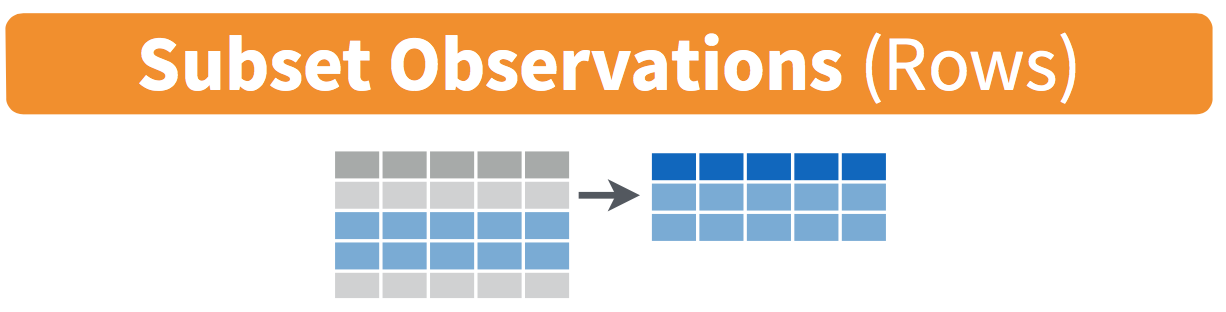
\includegraphics[width=\textwidth]{images/filter} 

}

\caption[Filter diagram from Data Wrangling with dplyr and tidyr cheatsheet]{Filter diagram from Data Wrangling with dplyr and tidyr cheatsheet}\label{fig:filter}
\end{figure}

The \texttt{filter} function here works much like the ``Filter'' option
in Microsoft Excel; it allows you to specify criteria about values of a
variable in your data set and then chooses only those rows that match
that criteria. We begin by focusing only on flights from New York City
to Portland, Oregon. The \texttt{dest} code (or airport code) for
Portland, Oregon is \texttt{"PDX"}. Run the following and look at the
resulting spreadsheet to ensure that only flights heading to Portland
are chosen here:

\begin{Shaded}
\begin{Highlighting}[]
\NormalTok{portland_flights <-}\StringTok{ }\NormalTok{flights %>%}\StringTok{ }
\StringTok{  }\KeywordTok{filter}\NormalTok{(dest ==}\StringTok{ "PDX"}\NormalTok{)}
\KeywordTok{View}\NormalTok{(pdx_flights)}
\end{Highlighting}
\end{Shaded}

Note the following:

\begin{itemize}
\tightlist
\item
  The ordering of the commands:

  \begin{itemize}
  \tightlist
  \item
    Take the data frame \texttt{flights} \emph{then}
  \item
    \texttt{filter} the data frame so that only those where the
    \texttt{dest} equals \texttt{"PDX"}.
  \end{itemize}
\item
  The double equal sign \texttt{==} You are almost guaranteed to make
  the mistake at least once of only including one equals sign. Let's see
  what happens when we make this error:
\end{itemize}

\begin{Shaded}
\begin{Highlighting}[]
\NormalTok{portland_flights <-}\StringTok{ }\NormalTok{flights %>%}\StringTok{ }
\StringTok{  }\KeywordTok{filter}\NormalTok{(}\DataTypeTok{dest =} \StringTok{"PDX"}\NormalTok{)}
\end{Highlighting}
\end{Shaded}

\begin{verbatim}
Error: filter() takes unnamed arguments. Do you need `==`?
\end{verbatim}

You can combine multiple criteria together using operators that make
comparisons:

\begin{itemize}
\tightlist
\item
  \texttt{\textbar{}} corresponds to ``or''
\item
  \texttt{\&} corresponds to ``and''
\end{itemize}

We can often skip the use of \texttt{\&} and just separate our
conditions with a comma. You'll see this in the example below.

In addition, you can use other mathematical checks (similar to
\texttt{==}):

\begin{itemize}
\tightlist
\item
  \texttt{\textgreater{}} corresponds to ``greater than''
\item
  \texttt{\textless{}} corresponds to ``less than''
\item
  \texttt{\textgreater{}=} corresponds to ``greater than or equal to''
\item
  \texttt{\textless{}=} corresponds to ``less than or equal to''
\item
  \texttt{!=} corresponds to ``not equal to''
\end{itemize}

To see many of these in action, let's select all flights that left JFK
airport heading to Burlington, Vermont (\texttt{"BTV"}) or Seattle,
Washington (\texttt{"SEA"}) in the months of October, November, or
December. Run the following

\begin{Shaded}
\begin{Highlighting}[]
\NormalTok{btv_sea_flights_fall <-}\StringTok{ }\NormalTok{flights %>%}\StringTok{ }
\StringTok{  }\KeywordTok{filter}\NormalTok{(origin ==}\StringTok{ "JFK"}\NormalTok{, (dest ==}\StringTok{ "BTV"} \NormalTok{|}\StringTok{ }\NormalTok{dest ==}\StringTok{ "SEA"}\NormalTok{), month >=}\StringTok{ }\DecValTok{10}\NormalTok{)}
\KeywordTok{View}\NormalTok{(btv_sea_flights_fall)}
\end{Highlighting}
\end{Shaded}

Note how even though colloquially speaking one might say ``all flights
leaving Burlington, Vermont \emph{and} Seattle, Washington'', in terms
of computer operations, we really mean ``all flights leaving Burlington,
Vermont \emph{or} Seattle, Washington'', because for a given row in the
data, \texttt{dest} can either be: ``BTV'', ``SEA'', something else, but
not ``BTV'' and ``SEA'' at the same time.

Another example uses the \texttt{!} to pick rows that \textbf{DON'T}
match a condition. Here we are selecting rows corresponding to flights
that didn't go to Burlington, VT or Seattle, WA.

\begin{Shaded}
\begin{Highlighting}[]
\NormalTok{not_BTV_SEA <-}\StringTok{ }\NormalTok{flights %>%}\StringTok{ }
\StringTok{  }\KeywordTok{filter}\NormalTok{(!(dest ==}\StringTok{ "BTV"} \NormalTok{|}\StringTok{ }\NormalTok{dest ==}\StringTok{ "SEA"}\NormalTok{))}
\KeywordTok{View}\NormalTok{(not_BTV_SEA)}
\end{Highlighting}
\end{Shaded}

\begin{center}\rule{0.5\linewidth}{\linethickness}\end{center}

\begin{learncheck}
\textbf{\emph{Learning check}}
\end{learncheck}

\textbf{(LC5.1)} What's another way using \texttt{!} we could filter
only the rows that are not to Burlington, VT nor Seattle, WA in the
\texttt{flights} data frame? Test this out using the code above.

\begin{center}\rule{0.5\linewidth}{\linethickness}\end{center}

\subsection{\texorpdfstring{Summarize variables using
\texttt{summarize}}{Summarize variables using summarize}}\label{summarize-variables-using-summarize}

\begin{figure}

{\centering 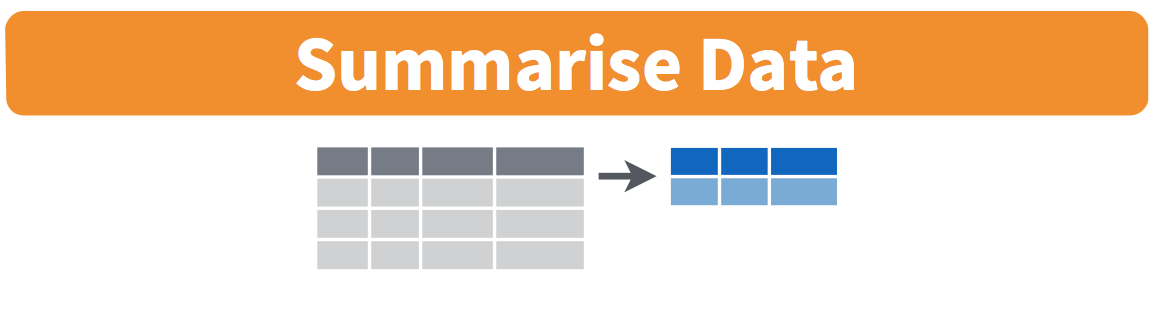
\includegraphics[width=\textwidth]{images/summarize1} 

}

\caption[Summarize diagram from Data Wrangling with dplyr and tidyr cheatsheet]{Summarize diagram from Data Wrangling with dplyr and tidyr cheatsheet}\label{fig:sum1}
\end{figure}

\begin{figure}

{\centering 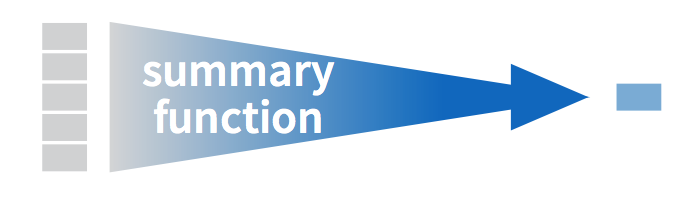
\includegraphics[width=\textwidth]{images/summary} 

}

\caption[Another summarize diagram from Data Wrangling with dplyr and tidyr cheatsheet]{Another summarize diagram from Data Wrangling with dplyr and tidyr cheatsheet}\label{fig:sum2}
\end{figure}

We saw in Subsection \ref{contsum} a way to calculate the standard
deviation and mean of the temperature variable \texttt{temp} in the
\texttt{weather} data frame of \texttt{nycflights}. We can do so in one
step using the \texttt{summarize} function in \texttt{dplyr}:

\begin{Shaded}
\begin{Highlighting}[]
\NormalTok{summary_temp <-}\StringTok{ }\NormalTok{weather %>%}\StringTok{ }
\StringTok{  }\KeywordTok{summarize}\NormalTok{(}\DataTypeTok{mean =} \KeywordTok{mean}\NormalTok{(temp), }\DataTypeTok{std_dev =} \KeywordTok{sd}\NormalTok{(temp))}
\NormalTok{summary_temp}
\end{Highlighting}
\end{Shaded}

\begin{verbatim}
## # A tibble: 1 × 2
##    mean std_dev
##   <dbl>   <dbl>
## 1    NA      NA
\end{verbatim}

We've created a small data frame here called \texttt{summary\_temp} that
includes both the \texttt{mean} and the \texttt{std\_dev} of the
\texttt{temp} variable in \texttt{weather}. By why are the mean and
standard deviation missing i.e. \texttt{NA}? Remember that by default
the \texttt{mean} and \texttt{sd} functions do not ignore missing
values. We need to specify the argument \texttt{na.rm=TRUE} (\texttt{rm}
is short for ``remove''):

\begin{Shaded}
\begin{Highlighting}[]
\NormalTok{summary_temp <-}\StringTok{ }\NormalTok{weather %>%}\StringTok{ }
\StringTok{  }\KeywordTok{summarize}\NormalTok{(}\DataTypeTok{mean =} \KeywordTok{mean}\NormalTok{(temp, }\DataTypeTok{na.rm =} \OtherTok{TRUE}\NormalTok{),}
            \DataTypeTok{std_dev =} \KeywordTok{sd}\NormalTok{(temp, }\DataTypeTok{na.rm =} \OtherTok{TRUE}\NormalTok{))}
\NormalTok{summary_temp}
\end{Highlighting}
\end{Shaded}

\begin{verbatim}
## # A tibble: 1 × 2
##       mean  std_dev
##      <dbl>    <dbl>
## 1 55.20351 17.78212
\end{verbatim}

Notice as shown in Figures \ref{fig:sum1} and \ref{fig:sum2}, the data
fram went from many rows to a single row of just the summary values.

If we'd like to access either of these values directly we can use the
\texttt{\$} to specify a column in a data frame:

\begin{Shaded}
\begin{Highlighting}[]
\NormalTok{summary_temp$mean}
\end{Highlighting}
\end{Shaded}

\begin{verbatim}
## [1] 55.20351
\end{verbatim}

\begin{Shaded}
\begin{Highlighting}[]
\NormalTok{summary_temp$std_dev}
\end{Highlighting}
\end{Shaded}

\begin{verbatim}
## [1] 17.78212
\end{verbatim}

However, it's often more useful to summarize a variable based on the
groupings of another variable. Let's say we were interested in the mean
and standard deviation of temperatures for each month. We believe that
you will be amazed at just how simple this is:

\begin{figure}

{\centering 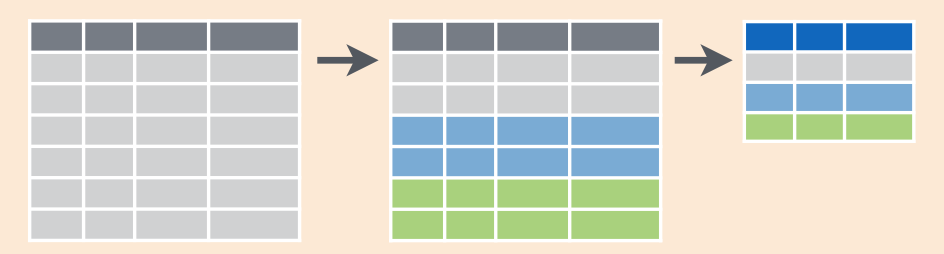
\includegraphics[width=\textwidth]{images/group_summary} 

}

\caption[Group by and summarize diagram from Data Wrangling with dplyr and tidyr cheatsheet]{Group by and summarize diagram from Data Wrangling with dplyr and tidyr cheatsheet}\label{fig:groupsummarize}
\end{figure}

Run the following code:

\begin{Shaded}
\begin{Highlighting}[]
\NormalTok{summary_monthly_temp <-}\StringTok{ }\NormalTok{weather %>%}\StringTok{ }
\StringTok{  }\KeywordTok{group_by}\NormalTok{(month) %>%}\StringTok{ }
\StringTok{  }\KeywordTok{summarize}\NormalTok{(}\DataTypeTok{mean =} \KeywordTok{mean}\NormalTok{(temp, }\DataTypeTok{na.rm =} \OtherTok{TRUE}\NormalTok{),}
            \DataTypeTok{std_dev =} \KeywordTok{sd}\NormalTok{(temp, }\DataTypeTok{na.rm =} \OtherTok{TRUE}\NormalTok{))}
\NormalTok{summary_monthly_temp}
\end{Highlighting}
\end{Shaded}

\begin{verbatim}
## # A tibble: 12 × 3
##    month     mean   std_dev
##    <dbl>    <dbl>     <dbl>
## 1      1 35.64127 10.185459
## 2      2 34.15454  6.940228
## 3      3 39.81404  6.224948
## 4      4 51.67094  8.785250
## 5      5 61.59185  9.608687
## 6      6 72.14500  7.603356
## 7      7 80.00967  7.147631
## 8      8 74.40495  5.171365
## 9      9 67.42582  8.475824
## 10    10 60.03305  8.829652
## 11    11 45.10893 10.502249
## 12    12 38.36811  9.940822
\end{verbatim}

Note that this code is identical to the previous code that created
\texttt{summary\_temp}, but there is an extra \texttt{group\_by(month)}
spliced in between. By simply grouping the \texttt{weather} data set by
\texttt{month} first and then passing this new data frame into
\texttt{summarize} we get a resulting data frame that shows the mean and
standard deviation temperature for each month in New York City.

What other summary functions can we use inside the \texttt{summarize()}
verb? Any function in R that takes a vector of values and returns just
one. Here are just a few:

\begin{itemize}
\tightlist
\item
  \texttt{min()} and \texttt{max()}: the minimum and maximum values
  respectively
\item
  \texttt{IQR()}: Interquartile range
\item
  \texttt{sum()}: the sum
\item
  \texttt{n()}: a count of how many entries appeared in the groupings.
\end{itemize}

Note there is a subtle but important difference between \texttt{sum()}
and \texttt{n()}. While \texttt{sum()} simply adds up a large set of
numbers, the latter counts the number of times different values occurs.
For example, suppose we'd like to get a sense for how many flights
departed each of the three airports in New York City:

\begin{Shaded}
\begin{Highlighting}[]
\NormalTok{by_origin <-}\StringTok{ }\NormalTok{flights %>%}\StringTok{ }
\StringTok{  }\KeywordTok{group_by}\NormalTok{(origin) %>%}\StringTok{ }
\StringTok{  }\KeywordTok{summarize}\NormalTok{(}\DataTypeTok{count =} \KeywordTok{n}\NormalTok{())}
\NormalTok{by_origin}
\end{Highlighting}
\end{Shaded}

\begin{verbatim}
## # A tibble: 3 × 2
##   origin  count
##    <chr>  <int>
## 1    EWR 120835
## 2    JFK 111279
## 3    LGA 104662
\end{verbatim}

We see that Newark (\texttt{"EWR"}) had the most flights departing in
2013 followed by \texttt{"JFK"} and lastly by LaGuardia
(\texttt{"LGA"}).

\begin{center}\rule{0.5\linewidth}{\linethickness}\end{center}

\begin{learncheck}
\textbf{\emph{Learning check}}
\end{learncheck}

\textbf{(LC5.2)} Recall from Chapter \ref{viz} when we looked at plots
of temperatures by months in NYC. What does the standard deviation
column in the \texttt{summary\_tempXmonth} data frame tell us about
temperatures in New York City throughout the year?

\textbf{(LC5.3)} What code would be required to get the mean and
standard deviation temperature for each day in 2013 for NYC?

\textbf{(LC5.4)} How could we identify how many flights left each of the
three airports in each of the months of 2013?

\begin{center}\rule{0.5\linewidth}{\linethickness}\end{center}

\subsection{\texorpdfstring{Create new variables/change old variables
using
\texttt{mutate}}{Create new variables/change old variables using mutate}}\label{create-new-variableschange-old-variables-using-mutate}

\begin{figure}

{\centering 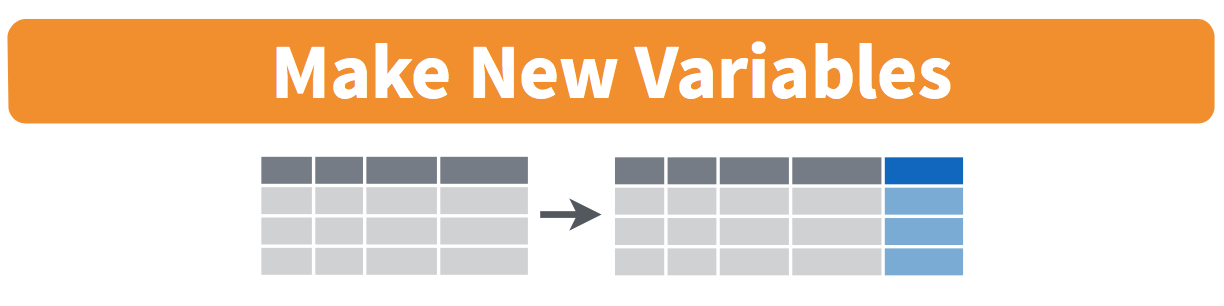
\includegraphics[width=\textwidth]{images/mutate} 

}

\caption[Mutate diagram from Data Wrangling with dplyr and tidyr cheatsheet]{Mutate diagram from Data Wrangling with dplyr and tidyr cheatsheet}\label{fig:select}
\end{figure}

When looking at the \texttt{flights} data set, there are some clear
additional variables that could be calculated based on the values of
variables already in the data set. Passengers are often frustrated when
their flights departs late, but change their mood a bit if pilots can
make up some time during the flight to get them to their destination
close to when they expected to land. This is commonly referred to as
``gain'' and we will create this variable using the \texttt{mutate}
function. Note that we have also overwritten the \texttt{flights} data
frame with what it was before as well as an additional variable
\texttt{gain} here.

\begin{Shaded}
\begin{Highlighting}[]
\NormalTok{flights <-}\StringTok{ }\NormalTok{flights %>%}\StringTok{ }
\StringTok{  }\KeywordTok{mutate}\NormalTok{(}\DataTypeTok{gain =} \NormalTok{arr_delay -}\StringTok{ }\NormalTok{dep_delay)}
\end{Highlighting}
\end{Shaded}

We can now look at summary measures of this \texttt{gain} variable and
even plot it in the form of a histogram:

\begin{Shaded}
\begin{Highlighting}[]
\NormalTok{gain_summary <-}\StringTok{ }\NormalTok{flights %>%}\StringTok{ }
\StringTok{  }\KeywordTok{summarize}\NormalTok{(}
    \DataTypeTok{min =} \KeywordTok{min}\NormalTok{(gain, }\DataTypeTok{na.rm =} \OtherTok{TRUE}\NormalTok{),}
    \DataTypeTok{q1 =} \KeywordTok{quantile}\NormalTok{(gain, }\FloatTok{0.25}\NormalTok{, }\DataTypeTok{na.rm =} \OtherTok{TRUE}\NormalTok{),}
    \DataTypeTok{median =} \KeywordTok{quantile}\NormalTok{(gain, }\FloatTok{0.5}\NormalTok{, }\DataTypeTok{na.rm =} \OtherTok{TRUE}\NormalTok{),}
    \DataTypeTok{q3 =} \KeywordTok{quantile}\NormalTok{(gain, }\FloatTok{0.75}\NormalTok{, }\DataTypeTok{na.rm =} \OtherTok{TRUE}\NormalTok{),}
    \DataTypeTok{max =} \KeywordTok{max}\NormalTok{(gain, }\DataTypeTok{na.rm =} \OtherTok{TRUE}\NormalTok{),}
    \DataTypeTok{mean =} \KeywordTok{mean}\NormalTok{(gain, }\DataTypeTok{na.rm =} \OtherTok{TRUE}\NormalTok{),}
    \DataTypeTok{sd =} \KeywordTok{sd}\NormalTok{(gain, }\DataTypeTok{na.rm =} \OtherTok{TRUE}\NormalTok{),}
    \DataTypeTok{missing =} \KeywordTok{sum}\NormalTok{(}\KeywordTok{is.na}\NormalTok{(gain))}
  \NormalTok{)}
\NormalTok{gain_summary}
\end{Highlighting}
\end{Shaded}

\begin{verbatim}
## # A tibble: 1 × 8
##     min    q1 median    q3   max      mean       sd missing
##   <dbl> <dbl>  <dbl> <dbl> <dbl>     <dbl>    <dbl>   <int>
## 1  -109   -17     -7     3   196 -5.659779 18.04365    9430
\end{verbatim}

We've recreated the \texttt{summary} function we saw in Chapter
\ref{viz} here using the \texttt{summarize} function in \texttt{dplyr}.

\begin{Shaded}
\begin{Highlighting}[]
\KeywordTok{ggplot}\NormalTok{(}\DataTypeTok{data =} \NormalTok{flights, }\DataTypeTok{mapping =} \KeywordTok{aes}\NormalTok{(}\DataTypeTok{x =} \NormalTok{gain)) +}
\StringTok{  }\KeywordTok{geom_histogram}\NormalTok{(}\DataTypeTok{color =} \StringTok{"white"}\NormalTok{, }\DataTypeTok{bins =} \DecValTok{20}\NormalTok{)}
\end{Highlighting}
\end{Shaded}

\begin{figure}

{\centering 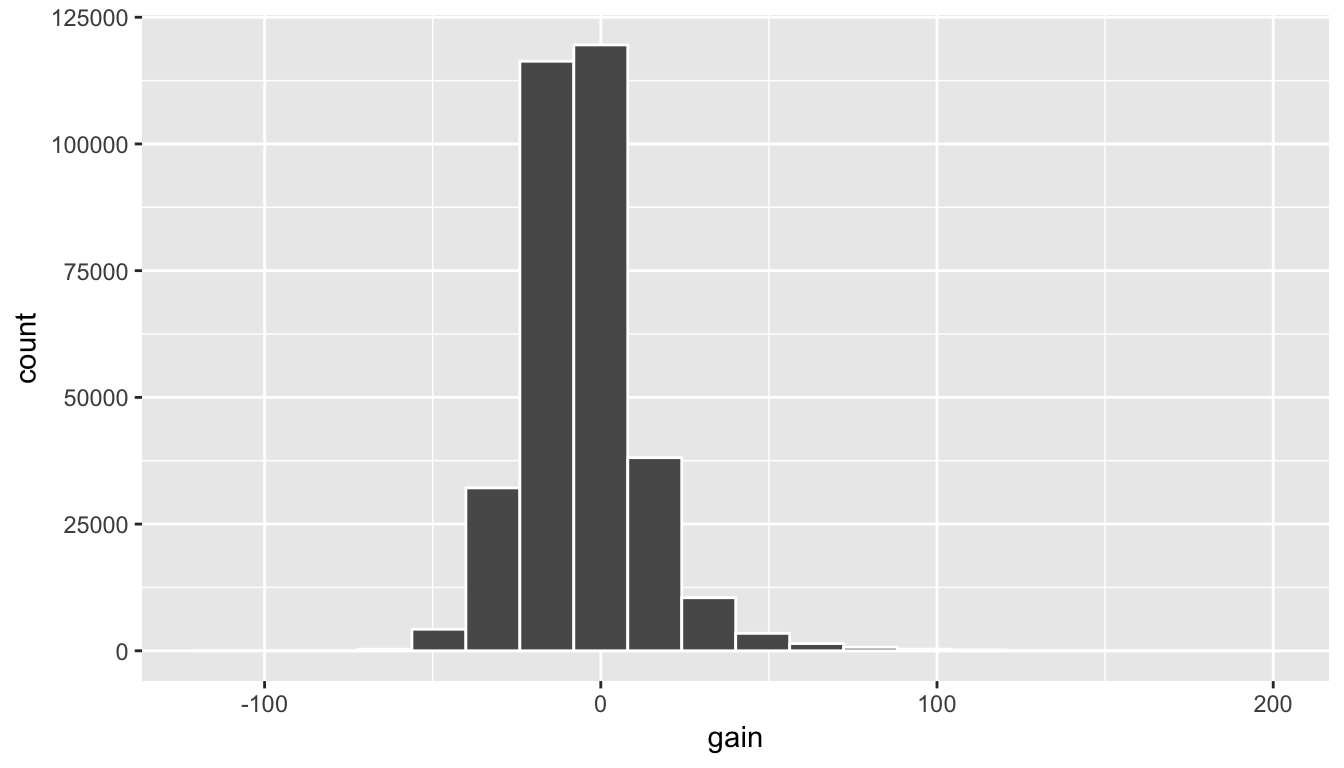
\includegraphics[width=\textwidth]{ismaykim_files/figure-latex/unnamed-chunk-39-1} 

}

\caption[Histogram of gain variable]{Histogram of gain variable}\label{fig:unnamed-chunk-39}
\end{figure}

We can also create multiple columns at once and even refer to columns
that were just created in a new column. Hadley produces one such example
in Chapter 5 of ``R for Data Science'' \citep{rds2016}:

\begin{Shaded}
\begin{Highlighting}[]
\NormalTok{flights_plus <-}\StringTok{ }\NormalTok{flights %>%}\StringTok{ }
\StringTok{  }\KeywordTok{mutate}\NormalTok{(}
    \DataTypeTok{gain =} \NormalTok{arr_delay -}\StringTok{ }\NormalTok{dep_delay,}
    \DataTypeTok{hours =} \NormalTok{air_time /}\StringTok{ }\DecValTok{60}\NormalTok{,}
    \DataTypeTok{gain_per_hour =} \NormalTok{gain /}\StringTok{ }\NormalTok{hours}
  \NormalTok{)}
\end{Highlighting}
\end{Shaded}

\begin{center}\rule{0.5\linewidth}{\linethickness}\end{center}

\begin{learncheck}
\textbf{\emph{Learning check}}
\end{learncheck}

\textbf{(LC5.5)} What do positive values of the \texttt{gain} variable
in \texttt{flights\_plus} correspond to? What about negative values? And
what about a zero value?

\textbf{(LC5.6)} Could we create the \texttt{dep\_delay} and
\texttt{arr\_delay} columns by simply subtracting \texttt{dep\_time}
from \texttt{sched\_dep\_time} and similarly for arrivals? Try the code
out and explain any differences between the result and what actually
appears in \texttt{flights}.

\textbf{(LC5.7)} What can we say about the distribution of
\texttt{gain}? Describe it in a few sentences using the plot and the
\texttt{gain\_summary} data frame values.

\begin{center}\rule{0.5\linewidth}{\linethickness}\end{center}

\subsection{\texorpdfstring{Reorder the data frame using
\texttt{arrange}}{Reorder the data frame using arrange}}\label{reorder-the-data-frame-using-arrange}

As you may have thought about with the data frames we've worked with so
far in the book, one of the most common things you'd like to do is sort
the data frames by a specific column. Have you ever been asked to
calculate a median by hand? This requires you to put the data in order
from smallest to highest in value. The \texttt{dplyr} package has a
function called \texttt{arrange} that we will use to sort/reorder our
data according to the values of the specified variable. This is most
frequently used after we have used the \texttt{group\_by} and
\texttt{summarize} functions as we will see.

Let's suppose we were interested in determining the most frequent
destination airports from New York City in 2013:

\begin{Shaded}
\begin{Highlighting}[]
\NormalTok{freq_dest <-}\StringTok{ }\NormalTok{flights %>%}\StringTok{ }
\StringTok{  }\KeywordTok{group_by}\NormalTok{(dest) %>%}\StringTok{ }
\StringTok{  }\KeywordTok{summarize}\NormalTok{(}\DataTypeTok{num_flights =} \KeywordTok{n}\NormalTok{())}
\NormalTok{freq_dest}
\end{Highlighting}
\end{Shaded}

\begin{verbatim}
## # A tibble: 105 × 2
##     dest num_flights
##    <chr>       <int>
## 1    ABQ         254
## 2    ACK         265
## 3    ALB         439
## 4    ANC           8
## 5    ATL       17215
## 6    AUS        2439
## 7    AVL         275
## 8    BDL         443
## 9    BGR         375
## 10   BHM         297
## # ... with 95 more rows
\end{verbatim}

You'll see that by default the values of \texttt{dest} are displayed in
alphabetical order here. Remember to use \texttt{View()} in the R
Console to look at all the values of \texttt{freq\_dest} in spreadsheet
format. We are interested in finding those airports that appear most:

\begin{Shaded}
\begin{Highlighting}[]
\NormalTok{freq_dest %>%}\StringTok{ }
\StringTok{  }\KeywordTok{arrange}\NormalTok{(num_flights)}
\end{Highlighting}
\end{Shaded}

\begin{verbatim}
## # A tibble: 105 × 2
##     dest num_flights
##    <chr>       <int>
## 1    LEX           1
## 2    LGA           1
## 3    ANC           8
## 4    SBN          10
## 5    HDN          15
## 6    MTJ          15
## 7    EYW          17
## 8    PSP          19
## 9    JAC          25
## 10   BZN          36
## # ... with 95 more rows
\end{verbatim}

This is actually giving us the opposite of what we are looking for. It
tells us the least frequent destination airports first. To switch the
ordering to be descending instead of ascending we use the \texttt{desc}
function:

\begin{Shaded}
\begin{Highlighting}[]
\NormalTok{freq_dest %>%}\StringTok{ }
\StringTok{  }\KeywordTok{arrange}\NormalTok{(}\KeywordTok{desc}\NormalTok{(num_flights))}
\end{Highlighting}
\end{Shaded}

\begin{verbatim}
## # A tibble: 105 × 2
##     dest num_flights
##    <chr>       <int>
## 1    ORD       17283
## 2    ATL       17215
## 3    LAX       16174
## 4    BOS       15508
## 5    MCO       14082
## 6    CLT       14064
## 7    SFO       13331
## 8    FLL       12055
## 9    MIA       11728
## 10   DCA        9705
## # ... with 95 more rows
\end{verbatim}

\subsection{Joining/merging data
frames}\label{joiningmerging-data-frames}

Something you may have thought to yourself as you looked at the most
freqent destinations of flights from NYC in 2013 is

\begin{itemize}
\tightlist
\item
  ``What cities are these airports in?''
\item
  ``Is \texttt{"ORD"} Orlando?''
\item
  ``Where is \texttt{"FLL"}?
\end{itemize}

The \texttt{nycflights13} data package contains multiple data frames.
Instead of having to manually look up different values of airport names
corresponding to airport codes like \texttt{ORD}, we can have R
automatically do this ``looking up'' for us. To do so, we'll need to
tell R how to match one data frame to another data frame. Let's first
check out the \texttt{airports} data frame inside of R:

\begin{Shaded}
\begin{Highlighting}[]
\KeywordTok{View}\NormalTok{(airports)}
\end{Highlighting}
\end{Shaded}

The first column \texttt{faa} corresponds to the airport codes that we
saw in \texttt{dest} in our \texttt{flights} and subsequent
\texttt{ten\_freq\_dests} data sets. Hadley and Garrett \citep{rds2016}
created the following diagram to help us understand how the different
data sets are linked:

\begin{figure}

{\centering 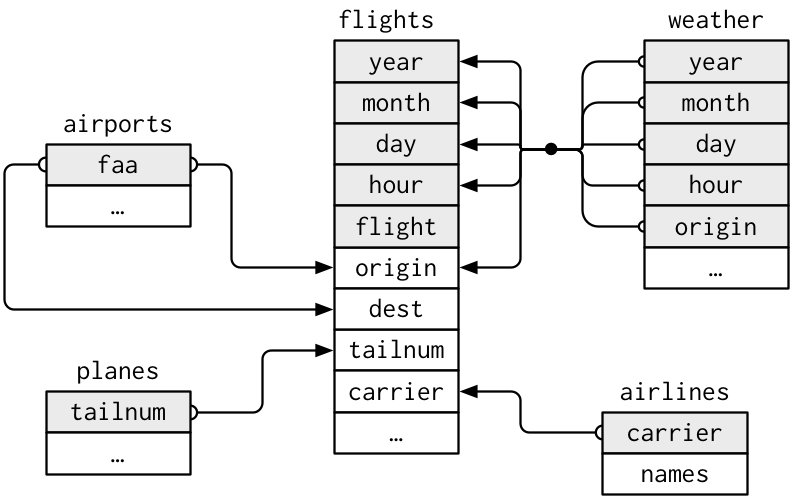
\includegraphics[width=\textwidth]{images/relational-nycflights} 

}

\caption[Data relationships in nycflights13 from R for Data Science]{Data relationships in nycflights13 from R for Data Science}\label{fig:reldiagram}
\end{figure}

We see from \texttt{View(airports)} that \texttt{airports} contains a
lot of other information about 1458. We are only really interested here
in the \texttt{faa} and \texttt{name} columns. Let's use the
\texttt{select} function to only use those variables:

\begin{Shaded}
\begin{Highlighting}[]
\NormalTok{airports_small <-}\StringTok{ }\NormalTok{airports %>%}\StringTok{ }\KeywordTok{select}\NormalTok{(faa, name)}
\end{Highlighting}
\end{Shaded}

So if we identify the names of the airports we can use the
\texttt{inner\_join} function to bring two different data frames
together. Note that we will also rename the subsequent column
\texttt{name} as \texttt{airport\_name}:

\begin{Shaded}
\begin{Highlighting}[]
\NormalTok{named_freq_dests <-}\StringTok{ }\NormalTok{flights %>%}
\StringTok{  }\KeywordTok{group_by}\NormalTok{(dest) %>%}
\StringTok{  }\KeywordTok{summarize}\NormalTok{(}\DataTypeTok{num_flights =} \KeywordTok{n}\NormalTok{()) %>%}
\StringTok{  }\KeywordTok{arrange}\NormalTok{(}\KeywordTok{desc}\NormalTok{(num_flights)) %>%}
\StringTok{  }\KeywordTok{inner_join}\NormalTok{(airports_small, }\DataTypeTok{by =} \KeywordTok{c}\NormalTok{(}\StringTok{"dest"} \NormalTok{=}\StringTok{ "faa"}\NormalTok{)) %>%}
\StringTok{  }\KeywordTok{rename}\NormalTok{(}\DataTypeTok{airport_name =} \NormalTok{name)}
\NormalTok{named_freq_dests}
\end{Highlighting}
\end{Shaded}

\begin{verbatim}
## # A tibble: 101 × 3
##     dest num_flights                       airport_name
##    <chr>       <int>                              <chr>
## 1    ORD       17283                 Chicago Ohare Intl
## 2    ATL       17215    Hartsfield Jackson Atlanta Intl
## 3    LAX       16174                   Los Angeles Intl
## 4    BOS       15508 General Edward Lawrence Logan Intl
## 5    MCO       14082                       Orlando Intl
## 6    CLT       14064             Charlotte Douglas Intl
## 7    SFO       13331                 San Francisco Intl
## 8    FLL       12055     Fort Lauderdale Hollywood Intl
## 9    MIA       11728                         Miami Intl
## 10   DCA        9705      Ronald Reagan Washington Natl
## # ... with 91 more rows
\end{verbatim}

In case you didn't know, \texttt{"ORD"} is the airport code of Chicago
O'Hare airport and \texttt{"FLL"} is the main airport in Fort
Lauderdale, Florida, which we can now see in our
\texttt{named\_freq\_dests} data frame.

A visual representation of the \texttt{inner\_join} is given below
\citep{rds2016}:

\begin{figure}

{\centering 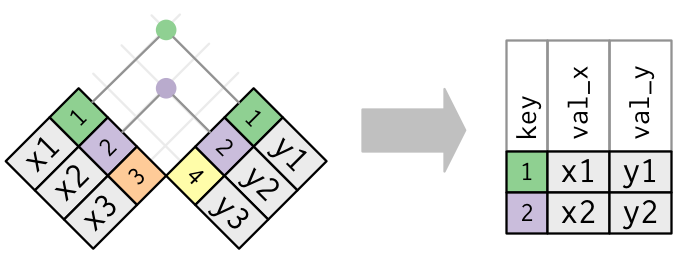
\includegraphics[width=\textwidth]{images/join-inner} 

}

\caption[Diagram of inner join from R for Data Science]{Diagram of inner join from R for Data Science}\label{fig:ijdiagram}
\end{figure}

There are more complex joins available, but the \texttt{inner\_join}
will solve nearly all of the problems you'll face in our experience.

\begin{center}\rule{0.5\linewidth}{\linethickness}\end{center}

\begin{learncheck}
\textbf{\emph{Learning check}}
\end{learncheck}

\textbf{(LC5.8)} What happens when you try to \texttt{inner\_join} the
\texttt{ten\_freq\_dests} data frame with \texttt{airports} instead of
\texttt{airports\_small}? How might one use this result to answer
further questions about the top 10 destinations?

\textbf{(LC5.9)} What surprises you about the top 10 destinations from
NYC in 2013?

\begin{center}\rule{0.5\linewidth}{\linethickness}\end{center}

\section{Other verbs}\label{other-verbs}

\subsection{\texorpdfstring{Select variables using
\texttt{select}}{Select variables using select}}\label{select-variables-using-select}

\begin{figure}

{\centering 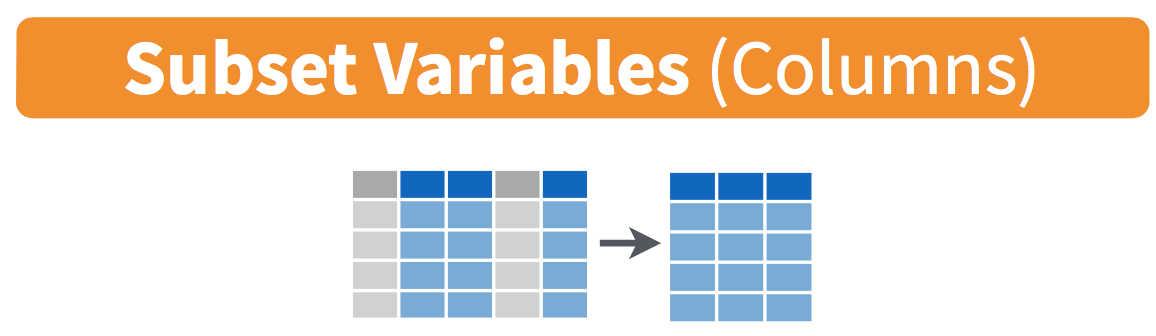
\includegraphics[width=\textwidth]{images/select} 

}

\caption[Select diagram from Data Wrangling with dplyr and tidyr cheatsheet]{Select diagram from Data Wrangling with dplyr and tidyr cheatsheet}\label{fig:selectfig}
\end{figure}

We've seen that the \texttt{flights} data frame in the
\texttt{nycflights13} package contains many different variables (19 in
fact). You can identify this by running the \texttt{dim} function or the
\texttt{ncol} function:

\begin{Shaded}
\begin{Highlighting}[]
\KeywordTok{data}\NormalTok{(flights)}
\KeywordTok{dim}\NormalTok{(flights)}
\end{Highlighting}
\end{Shaded}

\begin{verbatim}
## [1] 336776     19
\end{verbatim}

\begin{Shaded}
\begin{Highlighting}[]
\KeywordTok{ncol}\NormalTok{(flights)}
\end{Highlighting}
\end{Shaded}

\begin{verbatim}
## [1] 19
\end{verbatim}

One of these variables is \texttt{year}. If you remember the original
description of the \texttt{flights} data frame (or by running
\texttt{?flights}), you'll remember that this data correspond to flights
in 2013 departing New York City. The \texttt{year} variable isn't really
a variable here in that it doesn't vary\ldots{} \texttt{flights}
actually comes from a larger data set that covers many years. We may
want to remove the \texttt{year} variable from our data set since it
won't be helpful for analysis in this case. To do so easily, we use the
\texttt{select} variable:

\begin{Shaded}
\begin{Highlighting}[]
\NormalTok{flights_small <-}\StringTok{ }\NormalTok{flights %>%}\StringTok{ }
\StringTok{  }\KeywordTok{select}\NormalTok{(-year)}
\KeywordTok{names}\NormalTok{(flights_small)}
\end{Highlighting}
\end{Shaded}

\begin{verbatim}
##  [1] "month"          "day"            "dep_time"       "sched_dep_time"
##  [5] "dep_delay"      "arr_time"       "sched_arr_time" "arr_delay"     
##  [9] "carrier"        "flight"         "tailnum"        "origin"        
## [13] "dest"           "air_time"       "distance"       "hour"          
## [17] "minute"         "time_hour"
\end{verbatim}

The \texttt{names} function gives a listing of all the columns in a data
frame. We see that \texttt{year} has been removed. This was done using a
\texttt{-} in front of the name of the column we'd like to remove.

We could also select specific columns (instead of deselecting columns)
by listing them out:

\begin{Shaded}
\begin{Highlighting}[]
\NormalTok{flight_dep_times <-}\StringTok{ }\NormalTok{flights %>%}\StringTok{ }
\StringTok{  }\KeywordTok{select}\NormalTok{(month, day, dep_time, sched_dep_time)}
\NormalTok{flight_dep_times}
\end{Highlighting}
\end{Shaded}

\begin{verbatim}
## # A tibble: 336,776 × 4
##    month   day dep_time sched_dep_time
##    <int> <int>    <int>          <int>
## 1      1     1      517            515
## 2      1     1      533            529
## 3      1     1      542            540
## 4      1     1      544            545
## 5      1     1      554            600
## 6      1     1      554            558
## 7      1     1      555            600
## 8      1     1      557            600
## 9      1     1      557            600
## 10     1     1      558            600
## # ... with 336,766 more rows
\end{verbatim}

Or we could specify a ranges of columns:

\begin{Shaded}
\begin{Highlighting}[]
\NormalTok{flight_arr_times <-}\StringTok{ }\NormalTok{flights %>%}\StringTok{ }
\StringTok{  }\KeywordTok{select}\NormalTok{(month:day, arr_time:sched_arr_time)}
\NormalTok{flight_arr_times}
\end{Highlighting}
\end{Shaded}

\begin{verbatim}
## # A tibble: 336,776 × 4
##    month   day arr_time sched_arr_time
##    <int> <int>    <int>          <int>
## 1      1     1      830            819
## 2      1     1      850            830
## 3      1     1      923            850
## 4      1     1     1004           1022
## 5      1     1      812            837
## 6      1     1      740            728
## 7      1     1      913            854
## 8      1     1      709            723
## 9      1     1      838            846
## 10     1     1      753            745
## # ... with 336,766 more rows
\end{verbatim}

The \texttt{select} function can also be used to reorder columns in
combination with the \texttt{everything} helper function. Let's suppose
we'd like the \texttt{hour}, \texttt{minute}, and \texttt{time\_hour}
variables, which appear at the end of the \texttt{flights} data set, to
actually appear immediately after the \texttt{day} variable:

\begin{Shaded}
\begin{Highlighting}[]
\NormalTok{flights_reorder <-}\StringTok{ }\NormalTok{flights %>%}\StringTok{ }
\StringTok{  }\KeywordTok{select}\NormalTok{(month:day, hour:time_hour, }\KeywordTok{everything}\NormalTok{())}
\KeywordTok{names}\NormalTok{(flights_reorder)}
\end{Highlighting}
\end{Shaded}

\begin{verbatim}
##  [1] "month"          "day"            "hour"           "minute"        
##  [5] "time_hour"      "year"           "dep_time"       "sched_dep_time"
##  [9] "dep_delay"      "arr_time"       "sched_arr_time" "arr_delay"     
## [13] "carrier"        "flight"         "tailnum"        "origin"        
## [17] "dest"           "air_time"       "distance"
\end{verbatim}

Lastly, the helper functions \texttt{starts\_with}, \texttt{ends\_with},
and \texttt{contains} can be used to choose column names that match
those conditions:

\begin{Shaded}
\begin{Highlighting}[]
\NormalTok{flights_begin_a <-}\StringTok{ }\NormalTok{flights %>%}\StringTok{ }
\StringTok{  }\KeywordTok{select}\NormalTok{(}\KeywordTok{starts_with}\NormalTok{(}\StringTok{"a"}\NormalTok{))}
\NormalTok{flights_begin_a}
\end{Highlighting}
\end{Shaded}

\begin{verbatim}
## # A tibble: 336,776 × 3
##    arr_time arr_delay air_time
##       <int>     <dbl>    <dbl>
## 1       830        11      227
## 2       850        20      227
## 3       923        33      160
## 4      1004       -18      183
## 5       812       -25      116
## 6       740        12      150
## 7       913        19      158
## 8       709       -14       53
## 9       838        -8      140
## 10      753         8      138
## # ... with 336,766 more rows
\end{verbatim}

\begin{Shaded}
\begin{Highlighting}[]
\NormalTok{flights_delays <-}\StringTok{ }\NormalTok{flights %>%}\StringTok{ }
\StringTok{  }\KeywordTok{select}\NormalTok{(}\KeywordTok{ends_with}\NormalTok{(}\StringTok{"delay"}\NormalTok{))}
\NormalTok{flights_delays}
\end{Highlighting}
\end{Shaded}

\begin{verbatim}
## # A tibble: 336,776 × 2
##    dep_delay arr_delay
##        <dbl>     <dbl>
## 1          2        11
## 2          4        20
## 3          2        33
## 4         -1       -18
## 5         -6       -25
## 6         -4        12
## 7         -5        19
## 8         -3       -14
## 9         -3        -8
## 10        -2         8
## # ... with 336,766 more rows
\end{verbatim}

\begin{Shaded}
\begin{Highlighting}[]
\NormalTok{flights_time <-}\StringTok{ }\NormalTok{flights %>%}\StringTok{ }
\StringTok{  }\KeywordTok{select}\NormalTok{(}\KeywordTok{contains}\NormalTok{(}\StringTok{"time"}\NormalTok{))}
\NormalTok{flights_time}
\end{Highlighting}
\end{Shaded}

\begin{verbatim}
## # A tibble: 336,776 × 6
##    dep_time sched_dep_time arr_time sched_arr_time air_time
##       <int>          <int>    <int>          <int>    <dbl>
## 1       517            515      830            819      227
## 2       533            529      850            830      227
## 3       542            540      923            850      160
## 4       544            545     1004           1022      183
## 5       554            600      812            837      116
## 6       554            558      740            728      150
## 7       555            600      913            854      158
## 8       557            600      709            723       53
## 9       557            600      838            846      140
## 10      558            600      753            745      138
## # ... with 336,766 more rows, and 1 more variables: time_hour <dttm>
\end{verbatim}

\subsection{\texorpdfstring{Rename variables using
\texttt{rename}}{Rename variables using rename}}\label{rename-variables-using-rename}

Another useful function is \texttt{rename}, which as you may suspect
renames one column to another name. Suppose we wanted \texttt{dep\_time}
and \texttt{arr\_time} to be \texttt{departure\_time} and
\texttt{arrival\_time} instead in the \texttt{flights\_time} data frame:

\begin{Shaded}
\begin{Highlighting}[]
\NormalTok{flights_time <-}\StringTok{ }\NormalTok{flights_time %>%}\StringTok{ }
\StringTok{  }\KeywordTok{rename}\NormalTok{(}\DataTypeTok{departure_time =} \NormalTok{dep_time,}
         \DataTypeTok{arrival_time =} \NormalTok{arr_time)}
\KeywordTok{names}\NormalTok{(flights_time)}
\end{Highlighting}
\end{Shaded}

\begin{verbatim}
## [1] "departure_time" "sched_dep_time" "arrival_time"   "sched_arr_time"
## [5] "air_time"       "time_hour"
\end{verbatim}

It's easy to forget if the new name comes before or after the equals
sign. I usually remember this as ``New Before, Old After'' or NBOA.

You'll receive an error if you try to do it the other way:

\begin{verbatim}
Error: Unknown variables: departure_time, arrival_time.
\end{verbatim}

\begin{center}\rule{0.5\linewidth}{\linethickness}\end{center}

\begin{learncheck}
\textbf{\emph{Learning check}}
\end{learncheck}

\textbf{(LC5.10)} What are some ways to select all three of the
\texttt{dest}, \texttt{air\_time}, and \texttt{distance} variables from
\texttt{flights}? Give the code showing how to do this in at least three
different ways.

\textbf{(LC5.11)} How could one use \texttt{starts\_with},
\texttt{ends\_with}, and \texttt{contains} to select columns from the
\texttt{flights} data frame? Provide three different examples in total:
one for \texttt{starts\_with}, one for \texttt{ends\_with}, and one for
\texttt{contains}.

\textbf{(LC5.12)} Why might we want to use the \texttt{select} function
on a data frame?

\begin{center}\rule{0.5\linewidth}{\linethickness}\end{center}

\subsection{\texorpdfstring{Find the top number of values using
\texttt{top\_n}}{Find the top number of values using top\_n}}\label{find-the-top-number-of-values-using-top_n}

We can also use the \texttt{top\_n} function which automatically tells
us the most frequent \texttt{num\_flights}. We specify the top 10
airports here:

\begin{Shaded}
\begin{Highlighting}[]
\NormalTok{freq_dest %>%}\StringTok{ }
\StringTok{  }\KeywordTok{top_n}\NormalTok{(}\DataTypeTok{n =} \DecValTok{10}\NormalTok{, }\DataTypeTok{wt =} \NormalTok{num_flights)}
\end{Highlighting}
\end{Shaded}

\begin{verbatim}
## # A tibble: 10 × 2
##     dest num_flights
##    <chr>       <int>
## 1    ATL       17215
## 2    BOS       15508
## 3    CLT       14064
## 4    DCA        9705
## 5    FLL       12055
## 6    LAX       16174
## 7    MCO       14082
## 8    MIA       11728
## 9    ORD       17283
## 10   SFO       13331
\end{verbatim}

We'll still need to arrange this by \texttt{num\_flights} though:

\begin{Shaded}
\begin{Highlighting}[]
\NormalTok{freq_dest %>%}\StringTok{ }
\StringTok{  }\KeywordTok{top_n}\NormalTok{(}\DataTypeTok{n =} \DecValTok{10}\NormalTok{, }\DataTypeTok{wt =} \NormalTok{num_flights) %>%}\StringTok{ }
\StringTok{  }\KeywordTok{arrange}\NormalTok{(}\KeywordTok{desc}\NormalTok{(num_flights))}
\end{Highlighting}
\end{Shaded}

\begin{verbatim}
## # A tibble: 10 × 2
##     dest num_flights
##    <chr>       <int>
## 1    ORD       17283
## 2    ATL       17215
## 3    LAX       16174
## 4    BOS       15508
## 5    MCO       14082
## 6    CLT       14064
## 7    SFO       13331
## 8    FLL       12055
## 9    MIA       11728
## 10   DCA        9705
\end{verbatim}

\textbf{Note:} Remember that I didn't pull the \texttt{n} and
\texttt{wt} arguments out of thin air. They can be found by using the
\texttt{?} function on \texttt{top\_n}.

We can go one stop further and tie together the group\_by and summarize
functions we used to find the most frequent flights:

\begin{Shaded}
\begin{Highlighting}[]
\NormalTok{ten_freq_dests <-}\StringTok{ }\NormalTok{flights %>%}
\StringTok{  }\KeywordTok{group_by}\NormalTok{(dest) %>%}
\StringTok{  }\KeywordTok{summarize}\NormalTok{(}\DataTypeTok{num_flights =} \KeywordTok{n}\NormalTok{()) %>%}
\StringTok{  }\KeywordTok{top_n}\NormalTok{(}\DataTypeTok{n =} \DecValTok{10}\NormalTok{) %>%}
\StringTok{  }\KeywordTok{arrange}\NormalTok{(}\KeywordTok{desc}\NormalTok{(num_flights))}
\end{Highlighting}
\end{Shaded}

\begin{verbatim}
## Selecting by num_flights
\end{verbatim}

\begin{center}\rule{0.5\linewidth}{\linethickness}\end{center}

\begin{learncheck}
\textbf{\emph{Learning check}}
\end{learncheck}

\textbf{\texttt{paste0("(LC",\ chap,\ ".",\ (lc\ \textless{}-\ lc\ +\ 1),\ ")")}}
Create a new data frame that shows the top 5 airports with the largest
arrival delays from NYC in 2013.

\begin{center}\rule{0.5\linewidth}{\linethickness}\end{center}

\section{Conclusion}\label{conclusion-1}

\subsection{Resources}\label{resources-1}

As we saw with the RStudio cheatsheet on
\href{https://www.rstudio.com/wp-content/uploads/2015/12/ggplot2-cheatsheet-2.0.pdf}{data
visualization}, RStudio has also created a cheatsheet for data
manipulation entitled ``Data Wrangling with dplyr and tidyr'' available

\begin{itemize}
\tightlist
\item
  By clicking
  \href{https://www.rstudio.com/wp-content/uploads/2015/02/data-wrangling-cheatsheet.pdf}{here}
\item
  Or by clicking the RStudio Menu Bar -\textgreater{} Help
  -\textgreater{} Cheatsheets -\textgreater{} ``Data Manipulation with
  \texttt{dplyr}, \texttt{tidyr}''
\end{itemize}

We will focus only on the \texttt{dplyr} functions in this book, but you
are encouraged to also explore \texttt{tidyr} if you are presented with
data that is not in the tidy format that we have specified as the
preferred option for our purposes.

\subsection{Script of R code}\label{script-of-r-code-1}

An R script file of all R code used in this chapter is available
\href{http://ismayc.github.io/moderndiver-book/05-manip.R}{here}.

\subsection{What's to come?}\label{whats-to-come-2}

This concludes the \textbf{Data Exploration} unit of this book. You
should be pretty proficient in both plotting variables (or multiple
variables together) in various data sets and manipulating data as we've
done in this chapter. You are encouraged to step back through the code
in earlier chapters and make changes as you see fit based on your
updated knowledge.

In Chapter \ref{sim}, we'll begin to build the pieces needed to
understand how this unit of \textbf{Data Exploration} can tie into
statistical inference in the \textbf{Inference} part of the book.
Remember that the focus throughout is on data visualization and we'll
see that next when we discuss sampling, resampling, and bootstrapping.
These ideas will lead us into hypothesis testing and confidence
intervals.

\part{Inference}\label{part-inference}

\chapter{Simulating Randomness via mosaic}\label{sim}

In this chapter we will introduce new concepts that will serve as the
basis for the remainder of the text: \textbf{sampling} and
\textbf{resampling}. We will see that the tools that you learned in the
Data Exploration part of this book (tidy data, data manipulation, and
data visualization) will also play an important role here. As mentioned
before, the concepts all build into a culmination allowing you to create
better stories with data.

We begin with some helpful definitions that will help us better
understand why statistical inference exists and why it is needed. We
will then progress with introducing the second of our main data sets (in
addition to the \texttt{nycflights13} data you've been working with)
about OKCupid dating profiles to see how one can think of the
distribution of a sample being an approximation of the distribution of
the population. We will also focus on representative, random samples
versus convenience samples in this context.

We then shift to a famous example from statistics lore on a lady tasting
tea. This section will focus on introducing concepts without a lot of
statistical jargon. The chapter will conclude with a summary of the
different functions introduced in the \texttt{mosaic} package in this
chapter.

\section*{Needed packages}\label{needed-packages-2}
\addcontentsline{toc}{section}{Needed packages}

\begin{Shaded}
\begin{Highlighting}[]
\KeywordTok{library}\NormalTok{(dplyr)}
\KeywordTok{library}\NormalTok{(ggplot2)}
\KeywordTok{library}\NormalTok{(okcupiddata)}
\KeywordTok{library}\NormalTok{(mosaic)}
\KeywordTok{library}\NormalTok{(knitr)}
\end{Highlighting}
\end{Shaded}

\section{Random sampling}\label{random-sampling}

Whenever you hear the phrases ``random sampling'' or just ``sampling''
(with regards to statistics), you should think about tasting soup. This
likely sounds a little bonkers. Let's dig into why tasting soup is such
an excellent analogy to random sampling.

\subsection{Tasting soup}\label{tasting-soup}

\begin{figure}

{\centering 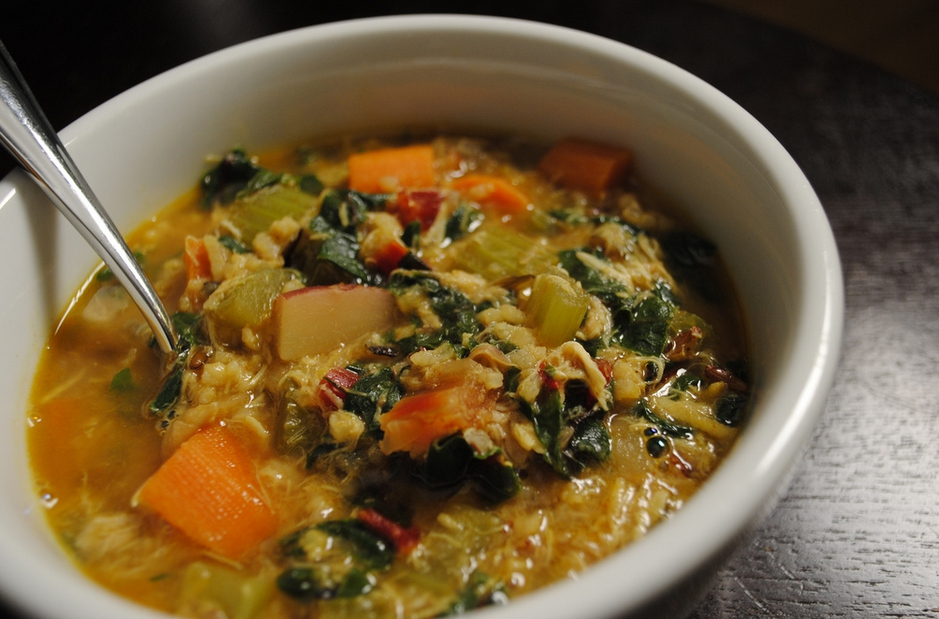
\includegraphics[width=\textwidth]{images/soup} 

}

\caption[A bowl of Indian chicken and vegetable soup]{A bowl of Indian chicken and vegetable soup}\label{fig:soupimg}
\end{figure}

Imagine that you have invited a group of friends over to try a new
recipe for soup that you've never made before. As in the image above
downloaded from
\href{http://readthespirit.wpengine.netdna-cdn.com/feed-the-spirit/wp-content/uploads/sites/19/2015/02/Chicken-soup-Indian-by-Fifth-Floor-Kitchen.jpg}{here},
you'd like to make a bowl of Indian chicken soup with lots of different
kinds of vegetables included.

You've carefully followed along with the recipe but you are concerned
that you don't have a lot of experience making foods from India. It is
coming near the end of the prescribed time to cook given in the recipe.
You begin to wonder:

\begin{itemize}
\tightlist
\item
  ``Did I add too much curry spice?''
\item
  ``Are the carrots cooked enough?''\\
\item
  ``Does this actually taste good?''
\end{itemize}

How can we answer these questions? Does it matter where we take a bite
of soup from? Is there anything we should do to the soup before we
taste? Is one taste enough?

\begin{center}\rule{0.5\linewidth}{\linethickness}\end{center}

\begin{learncheck}
\textbf{\emph{Learning check}}
\end{learncheck}

\textbf{(LC6.1)} Explain in your own words how tasting soup relates to
the concepts of sampling covered here.

\textbf{(LC6.2)} Describe a different scenario (not food or drink
related) that is analogous to sampling concepts covered here.

\begin{center}\rule{0.5\linewidth}{\linethickness}\end{center}

\subsection{Common terms}\label{common-terms}

The process of sampling brings with it many common terms that we define
now. As you read over these definitions, think about how they each apply
to the tasting soup example above.

\begin{center}\rule{0.5\linewidth}{\linethickness}\end{center}

\textbf{Definition: population}

The \emph{population} is the (usually) large pool of observational units
that we are interested in.

\textbf{Definition: sample}

A \emph{sample} is a smaller collection of observational units that is
selected from the population.

\textbf{Definition: sampling}

\emph{Sampling} refers to the process of selecting observations from a
population. There are both random and non-random ways this can be done.

\textbf{Definition: representative sample}

A sample is said be a \emph{representative sample} if the
characteristics of observational units selected are a good approximation
of the characteristics from the original population.

\textbf{Definition: bias}

\emph{Bias} corresponds to a favoring of one group in a population over
another group.

\textbf{Definition: generalizability}

\emph{Generalizability} refers to the largest group in which it makes
sense to make inferences about from the sample collected. This is
directly related to how the sample was selected.

\textbf{Definition: parameter}

A \emph{parameter} is a calculation based on one or more variables
measured in the population. Parameters are almost always denoted
symbolically using Greek letters such as \(\mu\), \(\pi\), \(\sigma\),
\(\rho\), and \(\beta\).

\textbf{Definition: statistic}

A \emph{statistic} is a calculated based on one or more variables
measured in the sample. Parameters are usually denoted by lower case
Arabic letters with other symbols added sometimes. These include
\(\bar{x}\), \(\hat{p}\), \(s\), \(p\), and \(b\).

\begin{center}\rule{0.5\linewidth}{\linethickness}\end{center}

Let's explore these terms for our tasting soup example:

\emph{Population} - the entire container of soup that we have cooked.

\emph{Sample} - any smaller portion of soup collected that isn't the
whole container of soup. We could say that each spoonful of soup
represents one sample.

\emph{Sampling} - the process of selecting spoonfuls from the container
of soup

\emph{Representative sample} - A sample we select will only be
representative if it tastes like what the soup tastes like in general.
If we only select a carrot in our spoonful, we might not have a
representative sample.

\emph{Bias} - As we noted with the carrot selection example above, we
may select a sample that is not representative. If you watch chefs cook
or if you frequently cook, you'll be sure to stir the soup before you
taste it.

\emph{Generalizability} - If we stir our soup before we taste a spoonful
(and if we make sure we don't just pick our favorite item in the soup),
results from our sample can be generalized (by and large) to the larger
pot of soup. When we say ``Yum! This is good!'' after a couple
spoonfuls, we can be pretty confident that each bowl of soup for our
friends will taste good too.

\emph{Parameter} - An example here is could be the proportion of curry
entered into the entire pot of soup. A measurement of how salty the pot
of soup is on average is also a parameter. How crunchy, on average, the
carrots are in the pot of soup is one more example.

\emph{Statistic} - To convert a parameter to a statistic, you need only
to think about the same measurement on a spoonful:

\begin{itemize}
\tightlist
\item
  The proportion of curry to non-curry in a spoonful of soup
\item
  How salty the spoonful of soup is that we collected as our sample
\item
  How crunchy the carrots are in our spoonful of soup
\end{itemize}

\begin{center}\rule{0.5\linewidth}{\linethickness}\end{center}

\begin{learncheck}
\textbf{\emph{Learning check}}
\end{learncheck}

\textbf{(LC6.3)} Why isn't our population all bowls of soup? All bowls
of Indian chicken soup?

\textbf{(LC6.4)} Describe a way in which we could select a sample of
flights from \texttt{nycflights13} that is not representative.

\textbf{(LC6.5)} If we treat all of the flights in \texttt{nycflights13}
as the population, give examples of three \emph{parameters} we could
calculate.

\textbf{(LC6.6)} If we treat all of the flights in \texttt{nycflights13}
as the population, give examples of three \emph{statistics} we could
calculate.

\textbf{(LC6.7)} What biases might we see if we only select flights to
Boston when we are interested in looking at mean flight delays from NYC?

\begin{center}\rule{0.5\linewidth}{\linethickness}\end{center}

\section{Visualizing sampling}\label{visualizing-sampling}

Let's explore how sampling and these other terms relate to working with
data and data visualization. Here we introduce the \texttt{okcupiddata}
R package. Note that permission to use this data to create the R package
was explicitly granted by OkCupid. More information about this package
is available \href{https://github.com/rudeboybert/okcupiddata}{here}.
The \texttt{profiles} data frame in this R data package contains data
about 59,946 OkCupid users who were living within 25 miles of San
Francisco, had active profiles on June 26, 2012, were online in the
previous year, and had at least one picture in their profile. We will be
focusing on the \texttt{height} variable, which corresponds to
self-reported heights of the individual on their profile. Note that this
is measured in inches.

\begin{Shaded}
\begin{Highlighting}[]
\KeywordTok{library}\NormalTok{(okcupiddata)}
\KeywordTok{data}\NormalTok{(profiles)}
\end{Highlighting}
\end{Shaded}

Let's take a look at the distribution of \texttt{height} using a
histogram and \texttt{ggplot2}:

\begin{Shaded}
\begin{Highlighting}[]
\KeywordTok{library}\NormalTok{(ggplot2)}
\KeywordTok{ggplot}\NormalTok{(}\DataTypeTok{data =} \NormalTok{profiles, }\DataTypeTok{mapping =} \KeywordTok{aes}\NormalTok{(}\DataTypeTok{x =} \NormalTok{height)) +}
\StringTok{  }\KeywordTok{geom_histogram}\NormalTok{(}\DataTypeTok{bins =} \DecValTok{20}\NormalTok{, }\DataTypeTok{color =} \StringTok{"white"}\NormalTok{)}
\end{Highlighting}
\end{Shaded}

\begin{center}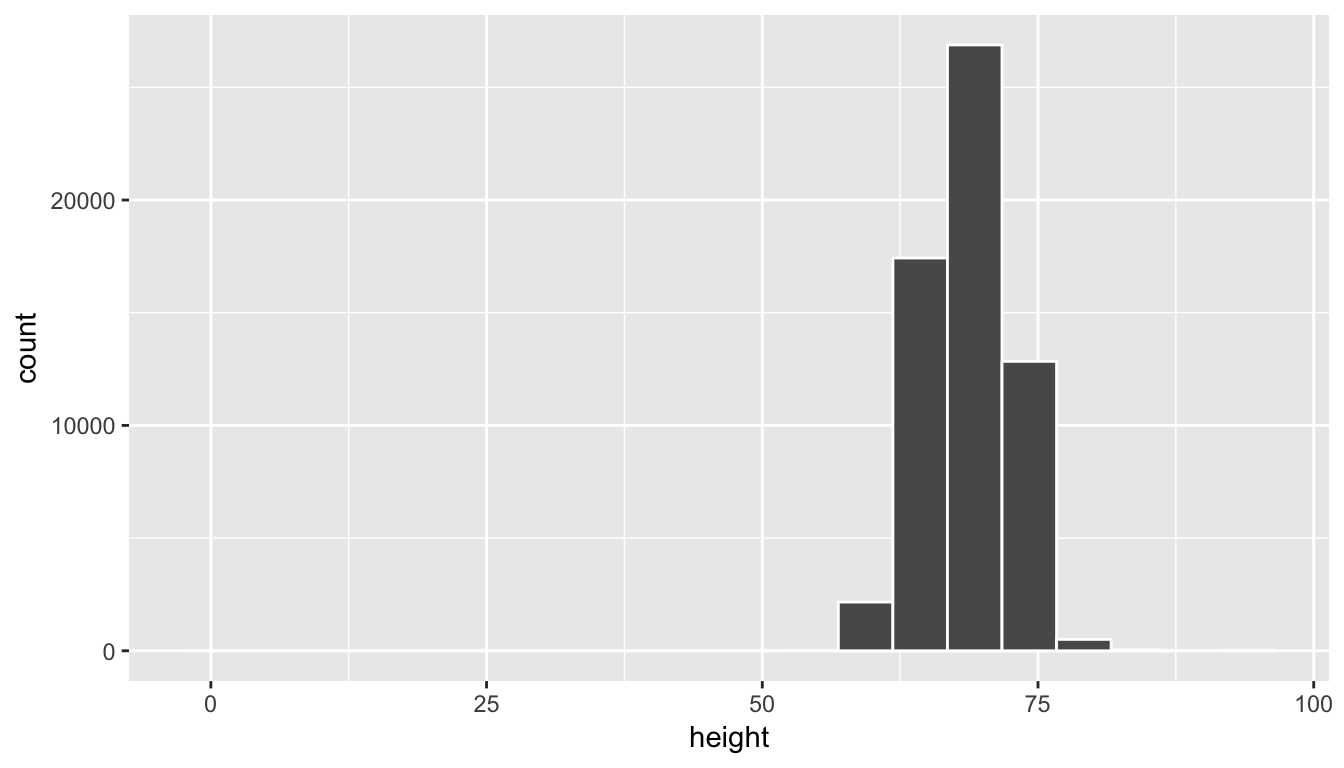
\includegraphics[width=\textwidth]{ismaykim_files/figure-latex/height-hist-1} \end{center}

We see here that this being self-reported data has led to the data being
a little messy.

\begin{center}\rule{0.5\linewidth}{\linethickness}\end{center}

\begin{learncheck}
\textbf{\emph{Learning check}}
\end{learncheck}

\textbf{(LC6.8)} Why does the histogram go all the way back to 0 for
height and all the way up to 100?

\begin{center}\rule{0.5\linewidth}{\linethickness}\end{center}

To clean up the data a bit, let's focus on just looking at heights
between 55 inches and 85 inches. Remember that the \texttt{filter}
function in \texttt{dplyr} allows us to focus on a subset of rows. The
specific subset of rows we are interested in corresponds to the argument
to the \texttt{filter} function. We will create a new data frame called
\texttt{profiles\_subset} that contains all rows with heights between 55
and 85 inclusive.

\begin{Shaded}
\begin{Highlighting}[]
\KeywordTok{library}\NormalTok{(dplyr)}
\NormalTok{profiles_subset <-}\StringTok{ }\NormalTok{profiles %>%}\StringTok{ }
\StringTok{  }\KeywordTok{filter}\NormalTok{(}\KeywordTok{between}\NormalTok{(height, }\DecValTok{55}\NormalTok{, }\DecValTok{85}\NormalTok{))}
\end{Highlighting}
\end{Shaded}

Next, let's produce the same histogram as above but using the
\texttt{profiles\_subset} data frame instead.

\begin{Shaded}
\begin{Highlighting}[]
\KeywordTok{library}\NormalTok{(ggplot2)}
\KeywordTok{ggplot}\NormalTok{(}\DataTypeTok{data =} \NormalTok{profiles_subset, }\DataTypeTok{mapping =} \KeywordTok{aes}\NormalTok{(}\DataTypeTok{x =} \NormalTok{height)) +}
\StringTok{  }\KeywordTok{geom_histogram}\NormalTok{(}\DataTypeTok{bins =} \DecValTok{20}\NormalTok{, }\DataTypeTok{color =} \StringTok{"white"}\NormalTok{)}
\end{Highlighting}
\end{Shaded}

\begin{center}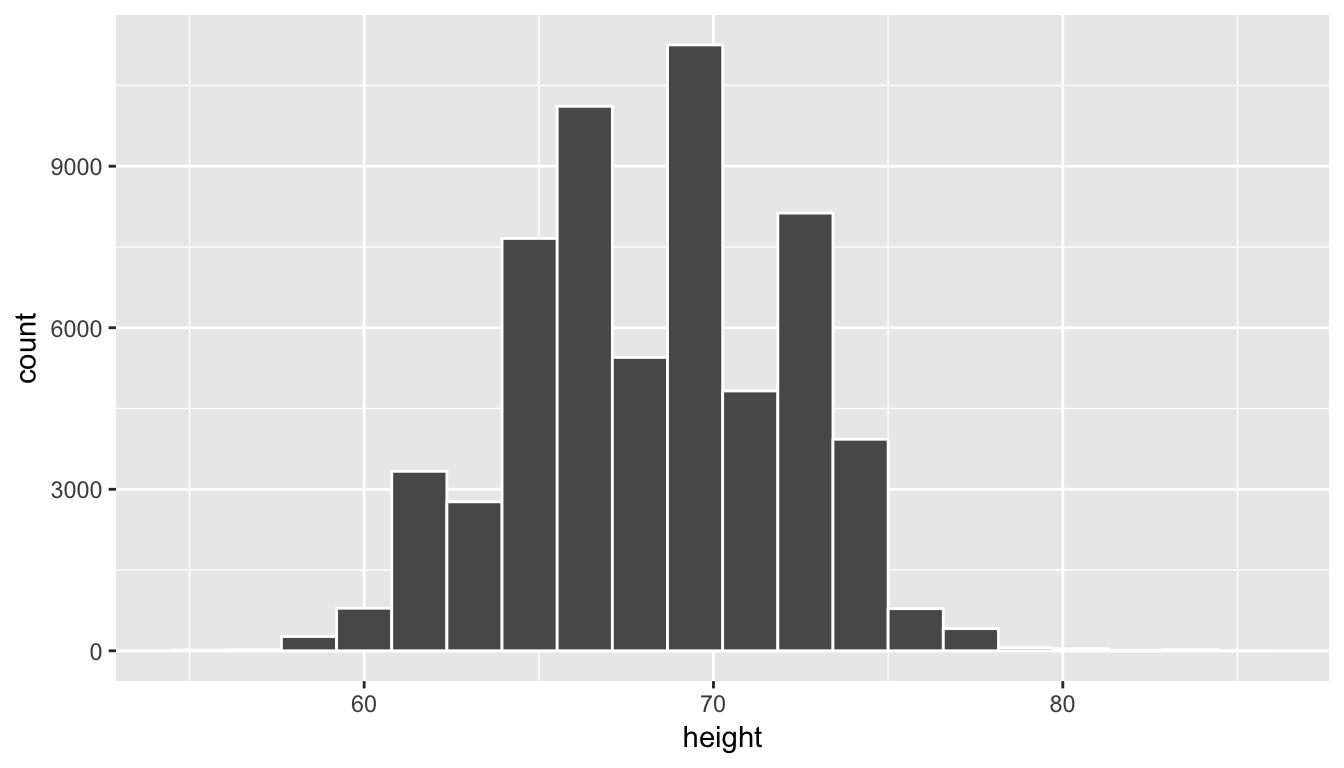
\includegraphics[width=\textwidth]{ismaykim_files/figure-latex/height-hist2-1} \end{center}

We can think of this data as representing the \emph{population} of
interest. Let's now take a random sample of size 100 from this
population and look to see if this sample represents the overall shape
of the population. In other words, we are going to use data
visualization as our guide to understand the \emph{representativeness}
of the sample selected.

\begin{Shaded}
\begin{Highlighting}[]
\KeywordTok{library}\NormalTok{(mosaic)}
\KeywordTok{set.seed}\NormalTok{(}\DecValTok{2017}\NormalTok{)}
\NormalTok{profiles_sample1 <-}\StringTok{ }\NormalTok{profiles_subset %>%}\StringTok{ }\KeywordTok{resample}\NormalTok{(}\DataTypeTok{size =} \DecValTok{100}\NormalTok{, }\DataTypeTok{replace =} \OtherTok{FALSE}\NormalTok{)}
\end{Highlighting}
\end{Shaded}

The \texttt{set.seed} function is used to ensure that all users get the
same random sample when they run the code above. It is a way of
interfacing with the pseudo-random number generation scheme that R uses
to generate ``random'' numbers. If that command was not run, you'd
obtain a different random sample if you ran the code above for the first
time.

We have introduced the \texttt{resample} function from the
\texttt{mosaic} package here. This function can be used for both
sampling with and without replacement. Here we have chosen to sample
without replacement. In other words, after the first row is chosen from
the \texttt{profiles\_subset} data frame at random it is kept out of the
further 99 samples. Let's now visualize the 100 values of the
\texttt{height} variable in the \texttt{profiles\_sample1} data frame.
To keep this visualization on the same horizontal scale as our original
population presented in \texttt{profiles\_subset} we can use the
\texttt{coord\_cartesian} function along with the \texttt{c} function to
specify the limits on the horizontal axis.

\begin{Shaded}
\begin{Highlighting}[]
\KeywordTok{ggplot}\NormalTok{(}\DataTypeTok{data =} \NormalTok{profiles_sample1, }\DataTypeTok{mapping =} \KeywordTok{aes}\NormalTok{(}\DataTypeTok{x =} \NormalTok{height)) +}
\StringTok{  }\KeywordTok{geom_histogram}\NormalTok{(}\DataTypeTok{bins =} \DecValTok{20}\NormalTok{, }\DataTypeTok{color =} \StringTok{"white"}\NormalTok{, }\DataTypeTok{fill =} \StringTok{"red"}\NormalTok{) +}
\StringTok{  }\KeywordTok{coord_cartesian}\NormalTok{(}\DataTypeTok{xlim =} \KeywordTok{c}\NormalTok{(}\DecValTok{55}\NormalTok{, }\DecValTok{85}\NormalTok{))}
\end{Highlighting}
\end{Shaded}

\begin{center}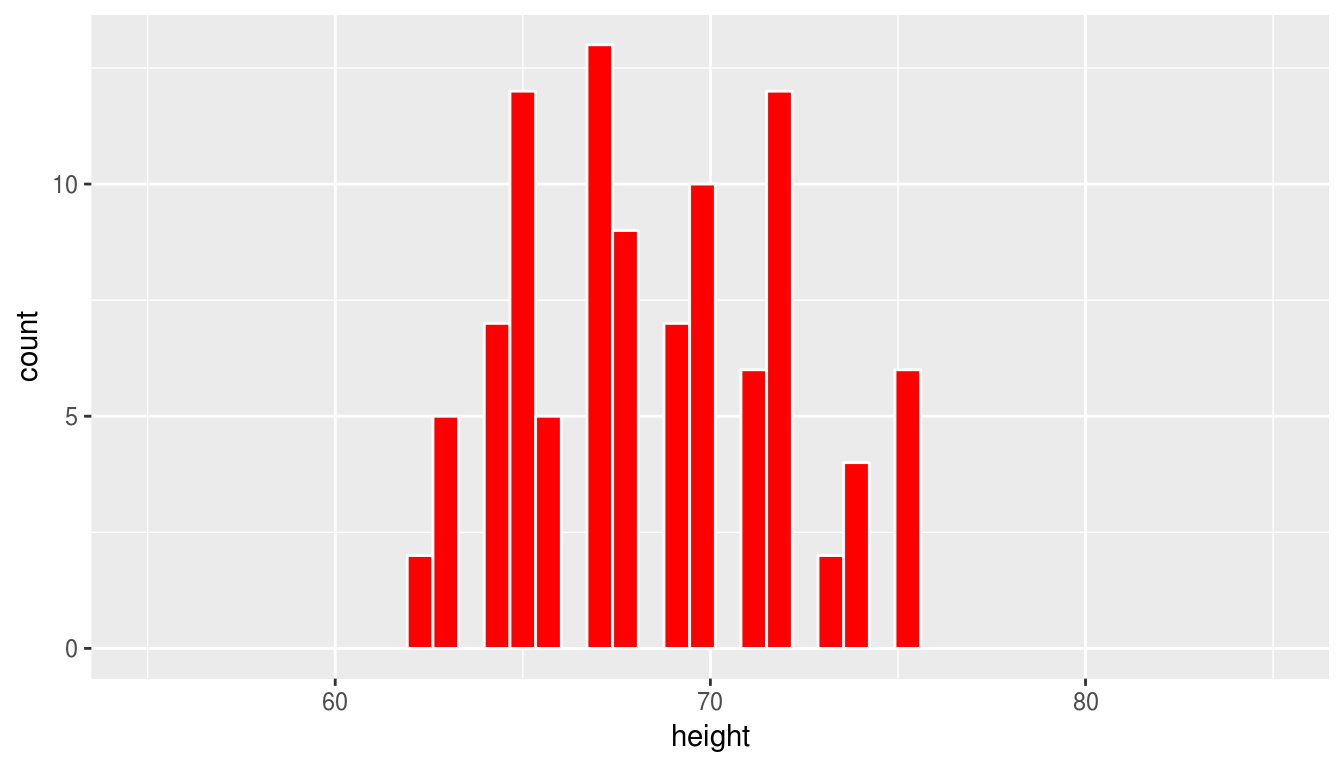
\includegraphics[width=\textwidth]{ismaykim_files/figure-latex/plot-sample1-1} \end{center}

\begin{center}\rule{0.5\linewidth}{\linethickness}\end{center}

\begin{learncheck}
\textbf{\emph{Learning check}}
\end{learncheck}

\textbf{(LC6.9)} Does this random sample of \texttt{height} represent
the population \texttt{height} variable well? Explain why or why not in
a couple of sentences.

\begin{center}\rule{0.5\linewidth}{\linethickness}\end{center}

We now repeat this process of sampling to look to see how another random
sample of \texttt{height} compares to the original population
distribution.

\begin{Shaded}
\begin{Highlighting}[]
\NormalTok{profiles_sample2 <-}\StringTok{ }\NormalTok{profiles_subset %>%}\StringTok{ }\KeywordTok{resample}\NormalTok{(}\DataTypeTok{size =} \DecValTok{100}\NormalTok{, }\DataTypeTok{replace =} \OtherTok{FALSE}\NormalTok{)}
\KeywordTok{ggplot}\NormalTok{(}\DataTypeTok{data =} \NormalTok{profiles_sample2, }\DataTypeTok{mapping =} \KeywordTok{aes}\NormalTok{(}\DataTypeTok{x =} \NormalTok{height)) +}
\StringTok{  }\KeywordTok{geom_histogram}\NormalTok{(}\DataTypeTok{bins =} \DecValTok{20}\NormalTok{, }\DataTypeTok{color =} \StringTok{"black"}\NormalTok{, }\DataTypeTok{fill =} \StringTok{"yellow"}\NormalTok{) +}
\StringTok{  }\KeywordTok{coord_cartesian}\NormalTok{(}\DataTypeTok{xlim =} \KeywordTok{c}\NormalTok{(}\DecValTok{55}\NormalTok{, }\DecValTok{85}\NormalTok{))}
\end{Highlighting}
\end{Shaded}

\begin{center}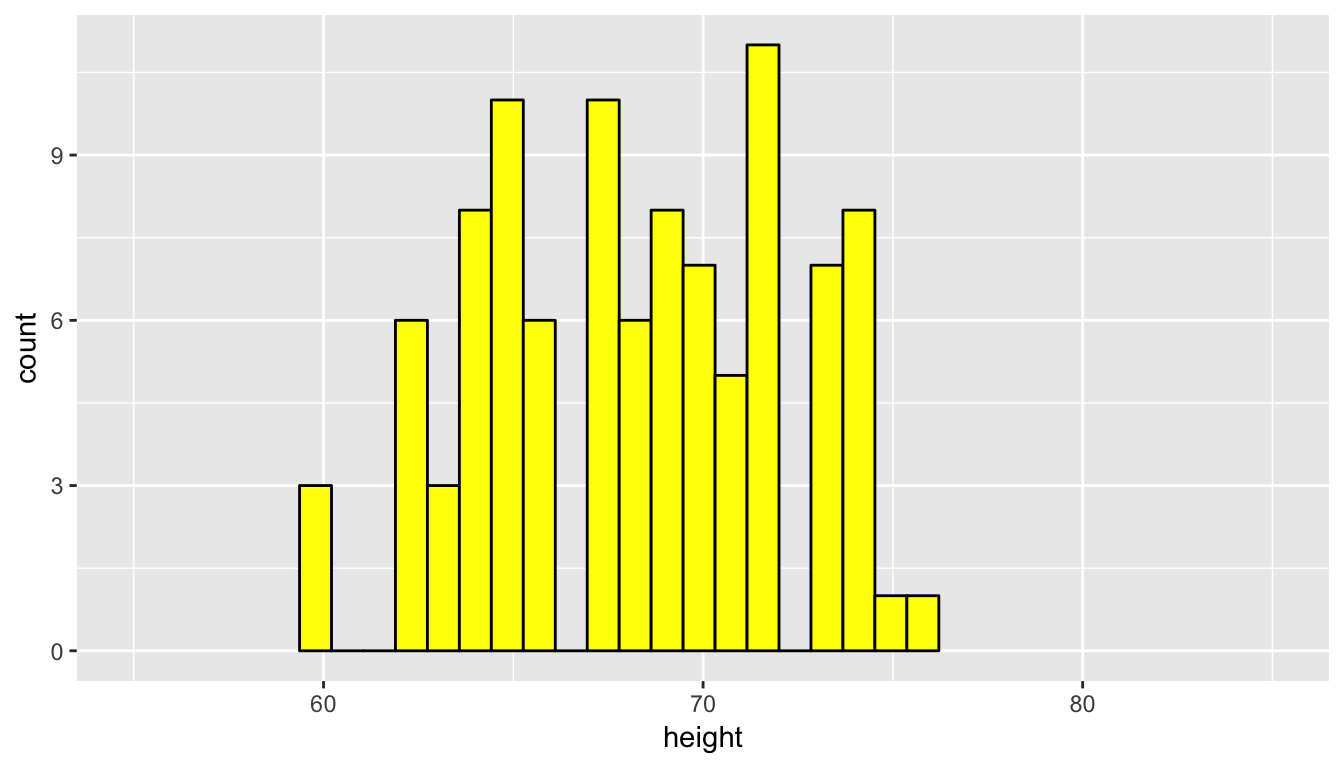
\includegraphics[width=\textwidth]{ismaykim_files/figure-latex/sample-profiles2-1} \end{center}

Remember that a sample can never truly quantify all of the properties of
a population since it contains less data and, thus, less information. We
can use the overall shape as a good guess as to the representativeness
of the sample in regards to the population. We see that the above two
random samples of size 100 have roughly the same shape as the original
population \texttt{height} data. Let's next explore what is known as a
convenience sample and how its distribution compares to the population
distribution.

A \textbf{convenience sample} is a sample that is chosen conveniently by
the person selecting the sample. While certainly less work, convenience
samples are generally not representative of the population since they
will exclude some (usually large) portion of the population. Let's look
at values of \texttt{height} in our \texttt{profiles\_subset} population
that are larger than 6 feet tall (72 inches) and have that be the sample
we choose.

\begin{Shaded}
\begin{Highlighting}[]
\NormalTok{profiles_sample3 <-}\StringTok{ }\NormalTok{profiles_subset %>%}\StringTok{ }
\StringTok{  }\KeywordTok{filter}\NormalTok{(height >=}\StringTok{ }\DecValTok{72}\NormalTok{)}
\KeywordTok{ggplot}\NormalTok{(}\DataTypeTok{data =} \NormalTok{profiles_sample3, }\DataTypeTok{mapping =} \KeywordTok{aes}\NormalTok{(}\DataTypeTok{x =} \NormalTok{height)) +}
\StringTok{  }\KeywordTok{geom_histogram}\NormalTok{(}\DataTypeTok{bins =} \DecValTok{20}\NormalTok{, }\DataTypeTok{color =} \StringTok{"white"}\NormalTok{, }\DataTypeTok{fill =} \StringTok{"blue"}\NormalTok{) +}
\StringTok{  }\KeywordTok{coord_cartesian}\NormalTok{(}\DataTypeTok{xlim =} \KeywordTok{c}\NormalTok{(}\DecValTok{55}\NormalTok{, }\DecValTok{85}\NormalTok{))}
\end{Highlighting}
\end{Shaded}

\begin{center}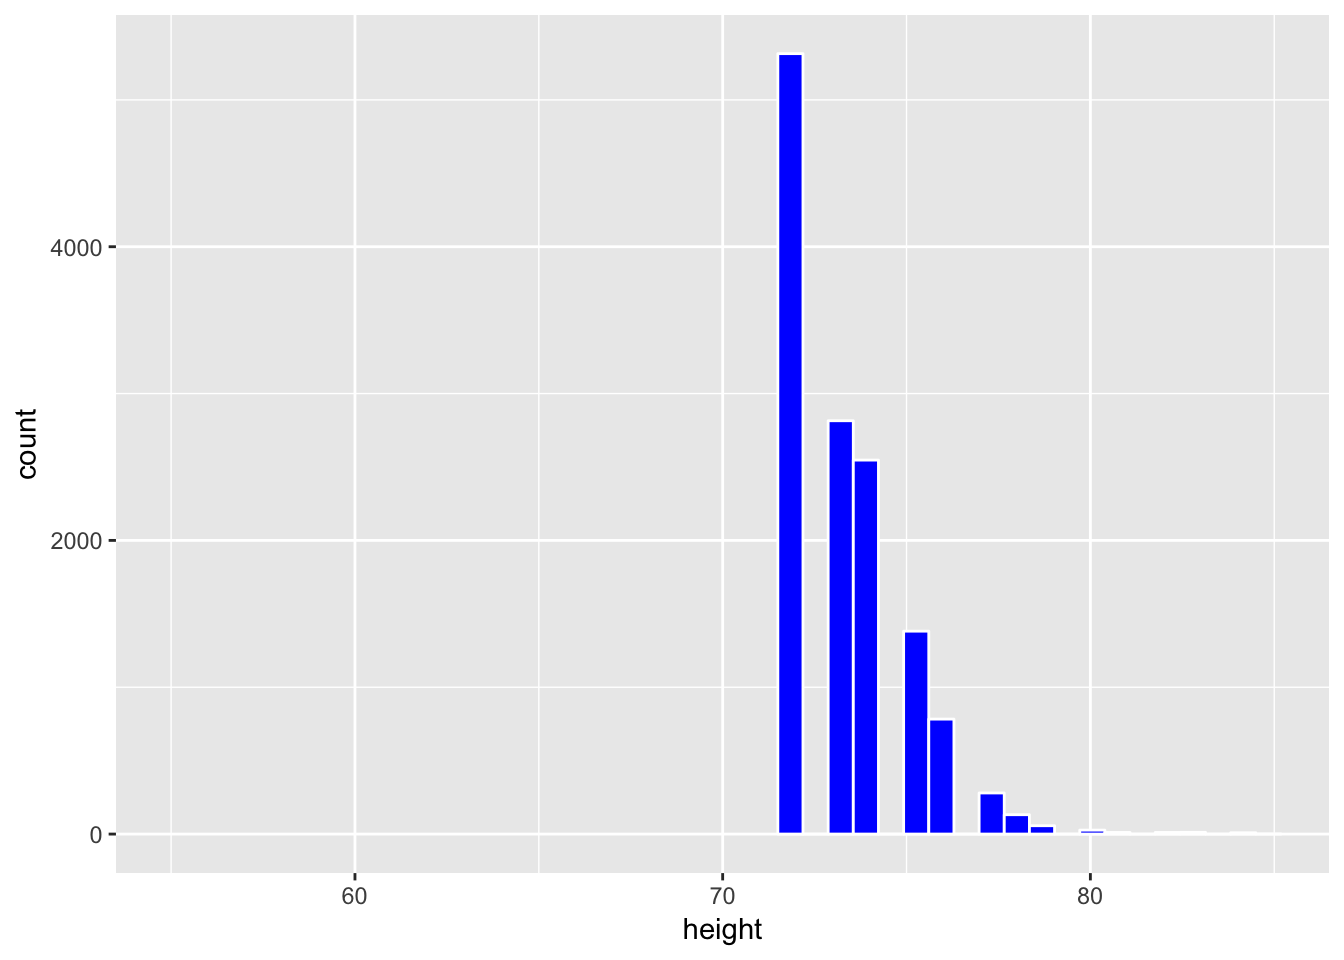
\includegraphics[width=\textwidth]{ismaykim_files/figure-latex/sample-profiles3-1} \end{center}

This is a clear example of a sample that is not representative of the
population. The population \texttt{height} is roughly symmetric, whereas
this distribution is right-skewed. Further, since it only selects large
heights it has completely excluded the small and middle heights. We have
seen here that data visualization provides an excellent tool in judging
the representativeness of a sample.

\subsection{Sampling distribution}\label{sampling-distribution}

The representativeness of a sample plays an even larger role than just
looking at the shapes of distributions. Let's suppose we were interested
in estimating the mean \texttt{height} of all profiles in the
\texttt{profiles\_subset} data frame. To do so, we could look at the
mean of the \texttt{height} variable in the \texttt{profiles\_sample1}
data frame:

\begin{Shaded}
\begin{Highlighting}[]
\NormalTok{profiles_sample1 %>%}\StringTok{ }\KeywordTok{summarize}\NormalTok{(}\KeywordTok{mean}\NormalTok{(height))}
\end{Highlighting}
\end{Shaded}

\begin{verbatim}
##   mean(height)
## 1        68.45
\end{verbatim}

But, we could also use \texttt{profiles\_sample2}:

\begin{Shaded}
\begin{Highlighting}[]
\NormalTok{profiles_sample2 %>%}\StringTok{ }\KeywordTok{summarize}\NormalTok{(}\KeywordTok{mean}\NormalTok{(height))}
\end{Highlighting}
\end{Shaded}

\begin{verbatim}
##   mean(height)
## 1         68.2
\end{verbatim}

Or maybe even \texttt{profiles\_sample3}:

\begin{Shaded}
\begin{Highlighting}[]
\NormalTok{profiles_sample3 %>%}\StringTok{ }\KeywordTok{summarize}\NormalTok{(}\KeywordTok{mean}\NormalTok{(height))}
\end{Highlighting}
\end{Shaded}

\begin{verbatim}
##   mean(height)
## 1     73.37917
\end{verbatim}

We see a clear difference here in looking at the mean of \texttt{height}
in \texttt{profiles\_sample3} versus \texttt{profiles\_sample1} and
\texttt{profiles\_sample2}. This comes from the bias that is used in
choosing only the top heights for \texttt{profiles\_sample3}. If we had
chosen to use this sample as our only sample, we would be quite a ways
off from what the actual mean \texttt{height} in our population of
\texttt{profiles\_subset} is.

We also see that even random samples produce means that aren't exactly
the same. This sampling variability can be shown via what is called a
\emph{sampling distribution}. This is defined as the behavior of a
statistic under repeated sampling. To build this sampling distribution
for this example, we've created an interactive app using the
\texttt{shiny} R package below that is available at
\url{http://ismay.shinyapps.io/okcupidheights/}. You can specify the
sample size you'd like to work with (100 is chosen by default) and then
generate a random sample. You then can see the mean of this generated
sample plotted in the bottom visualization. Repeating this process many
times, you can start to see the shape of the sampling distribution take
form.

\begin{figure}

{\centering 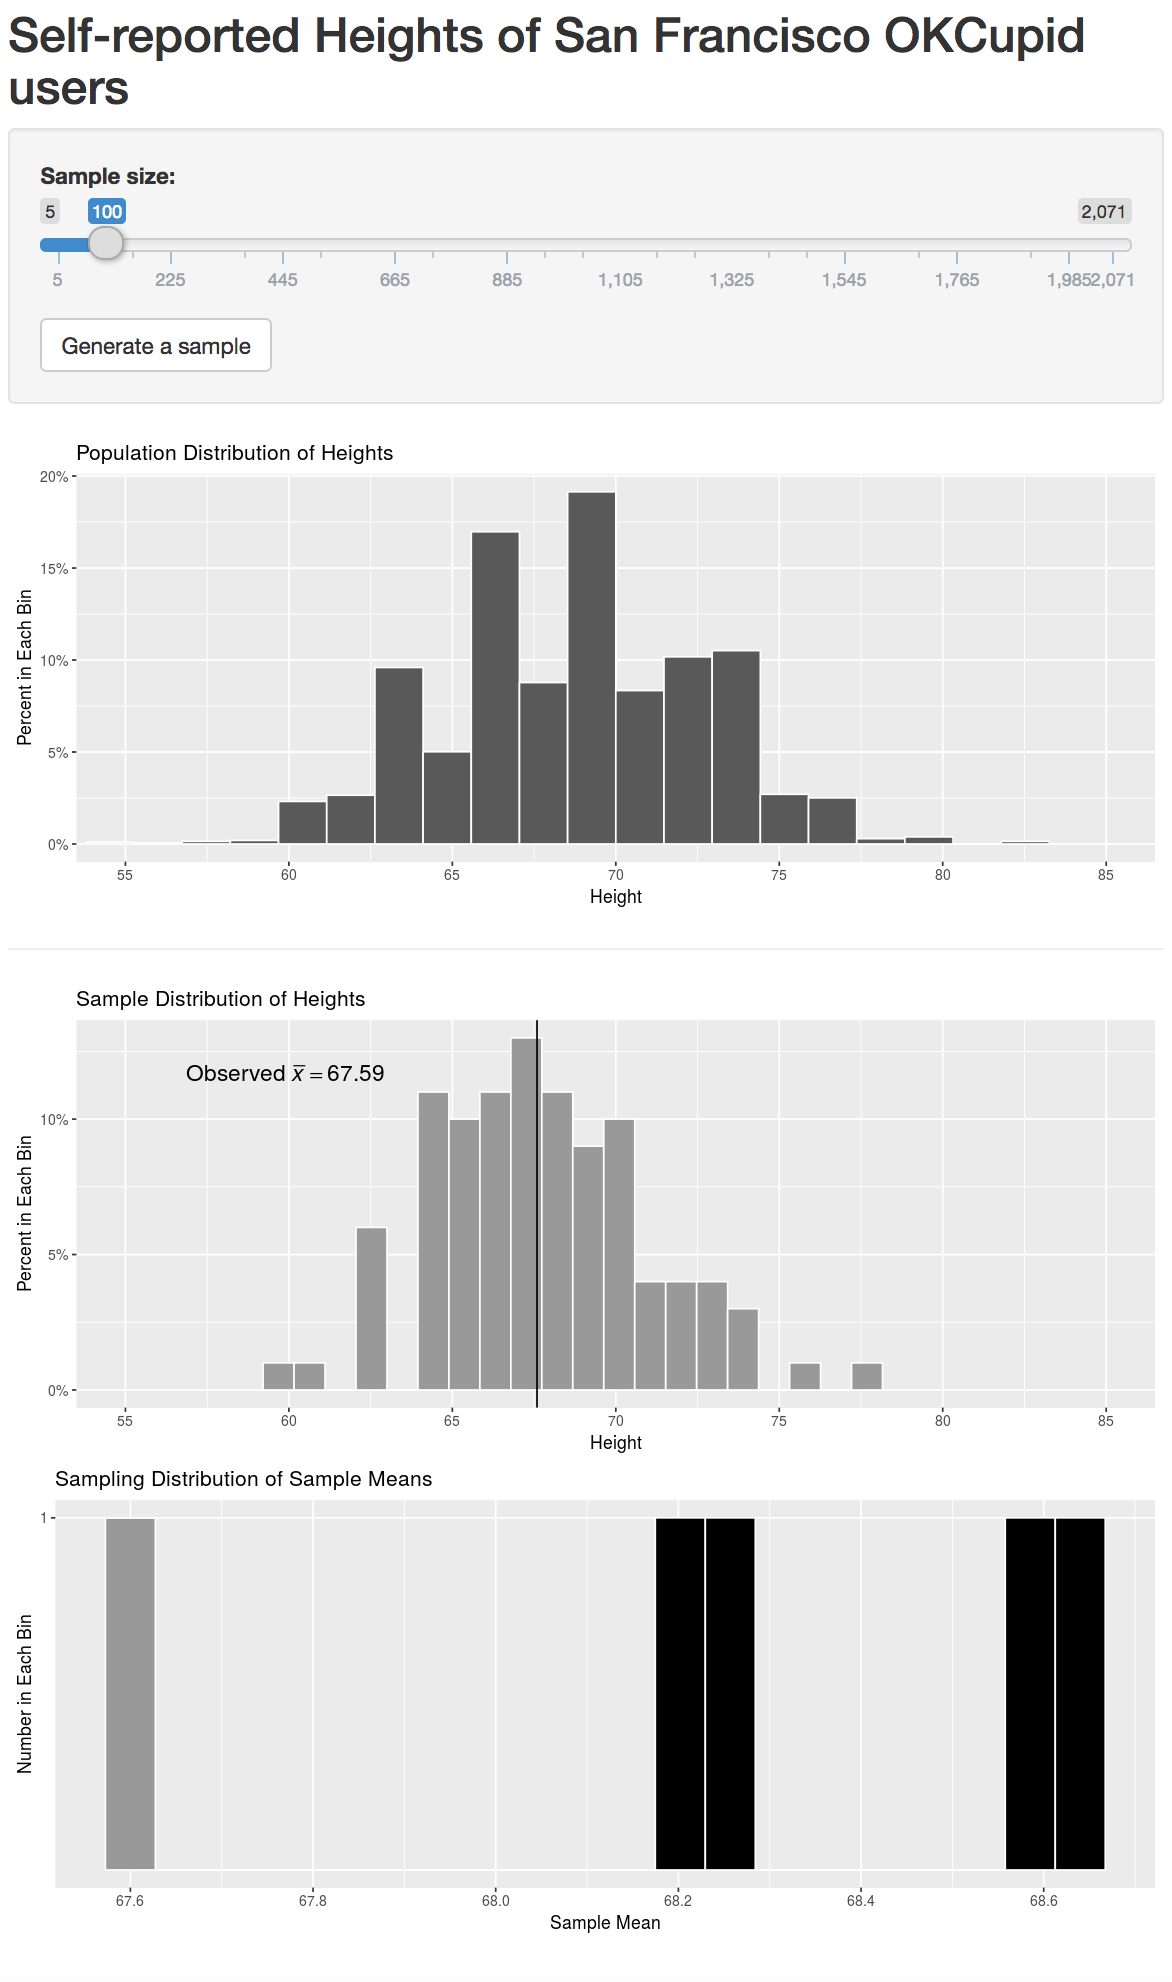
\includegraphics[width=1\linewidth]{images/shinyapp} 

}

\caption[Sampling distribution app]{Sampling distribution app}\label{fig:shiny}
\end{figure}

\subsection{\texorpdfstring{Repeated sampling via
\texttt{do}}{Repeated sampling via do}}\label{repeated-sampling-via-do}

We have looked at two random samples above, but using \texttt{mosaic} we
can repeat this process over and over again with the \texttt{do}
function. Below, we repeat this sampling process 10,000 times. We can
then plot the different values of the sample means to get a sense for
what a reasonable range of values for the population parameter mean
\texttt{height} is in the \texttt{profiles\_subset} data frame.

\begin{Shaded}
\begin{Highlighting}[]
\NormalTok{sample_means <-}\StringTok{ }\KeywordTok{do}\NormalTok{(}\DecValTok{10000}\NormalTok{) *}
\StringTok{  }\NormalTok{(profiles_subset %>%}\StringTok{ }\KeywordTok{resample}\NormalTok{(}\DataTypeTok{size =} \DecValTok{100}\NormalTok{, }\DataTypeTok{replace =} \OtherTok{FALSE}\NormalTok{) %>%}\StringTok{ }
\StringTok{  }\KeywordTok{summarize}\NormalTok{(}\DataTypeTok{mean_height =} \KeywordTok{mean}\NormalTok{(height)))}
\KeywordTok{ggplot}\NormalTok{(}\DataTypeTok{data =} \NormalTok{sample_means, }\DataTypeTok{mapping =} \KeywordTok{aes}\NormalTok{(}\DataTypeTok{x =} \NormalTok{mean_height)) +}
\StringTok{  }\KeywordTok{geom_histogram}\NormalTok{(}\DataTypeTok{color =} \StringTok{"white"}\NormalTok{, }\DataTypeTok{bins =} \DecValTok{20}\NormalTok{)}
\end{Highlighting}
\end{Shaded}

\begin{center}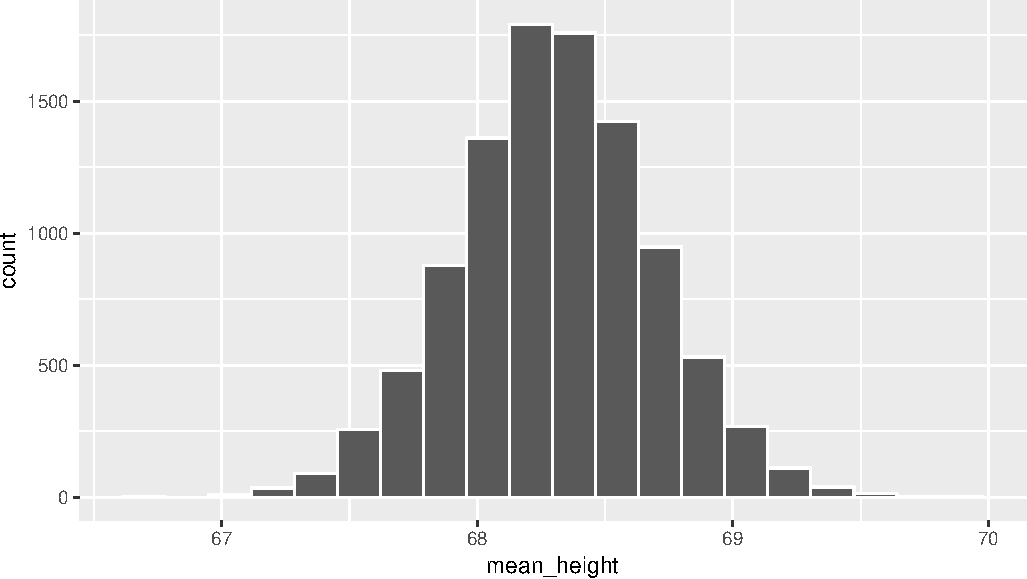
\includegraphics[width=\textwidth]{ismaykim_files/figure-latex/do-first-1} \end{center}

Note how the range of sample mean height values is much more narrow than
the original range of \texttt{height} in the \texttt{profiles\_subset}
data frame. We also see a characteristic shape to this distribution of
\texttt{sample\_mean}: the normal curve. This idea is commonly
associated with statistics and you hopefully have a good sense of how
this distribution comes about. As before, if you aren't quite sure of
this yet, go back and explore the shiny app above a bit more. We see
that many values for the sample mean appear near the center of the
distribution and a few values out in the tails providing the bell-shaped
distribution linked with the normal distribution. You'll see more
examples of this in the chapters to come and in the appendices.

\begin{center}\rule{0.5\linewidth}{\linethickness}\end{center}

\begin{learncheck}
\textbf{\emph{Learning check}}
\end{learncheck}

\textbf{(LC6.10)} Why do the sample mean values have a much smaller
spread than the original population data? You may want to play with the
shiny app above a bit to understand why this is the case.

\textbf{(LC6.11)} Why is random sampling so important here to create a
distribution of sample means that provide a range of plausible values
for the population mean height?

\begin{center}\rule{0.5\linewidth}{\linethickness}\end{center}

\section{Simulation}\label{simulation}

We next will introduce the ideas behind hypothesis testing that we will
delve into more formally in the chapters to come. What follows is taken
from a book entitled \emph{The Lady Tasting Tea} \citep{salsburg2001}:

\begin{quote}
It was a summer afternoon in Cambridge, England, in the late 1920s. A
group of university dons, their wives, and some guests were sitting
around an outdoor table for afternoon tea. One of the women was
insisting that tea tasted different depending upon whether the tea was
poured into the milk or whether the milk was poured into the tea. The
scientific minds among the men scoffed at this as sheer nonsense. What
could be the difference? They could not conceive of any difference in
the chemistry of the mixtures that could exist. A thin, short man, with
thick glasses and a Vandyke beard beginning to turn gray, pounced on the
problem. ``Let us test the proposition,'' he said excitedly. He began to
outline an experiment in which the lady who insisted there was a
difference would be presented with a sequence of cups of tea, in some of
which the milk had been poured into the tea and in others of which the
tea had been poured into the milk\ldots{}
\end{quote}

\begin{quote}
So it was that sunny summer afternoon in Cambridge. The lady might or
might not have been correct about the tea infusion. The fun would be in
finding a way to determine if she was right, and, under the direction of
the man with the Vandyke beard, they began to discuss how they might
make that determination.
\end{quote}

\begin{quote}
Enthusiastically, many of them joined with him in setting up the
experiment. Within a few minutes, they were pouring different patterns
of infusion in a place where the lady could not see which cup was which.
Then, with an air of finality, the man with the Vandyke beard presented
her with her first cup. She sipped for a minute and declared that it was
one where the milk had been poured into the tea. He noted her response
without comment and presented her with the second cup\ldots{}
\end{quote}

\begin{quote}
The man with the Vandyke beard was Ronald Aylmer Fisher, who was in his
late thirties at the time. He would later be knighted Sir Ronald Fisher.
In 1935, he wrote a book entitled \emph{The Design of Experiments}, and
he described the experiment of the lady tasting tea in the second
chapter of that book. In his book, Fisher discusses the lady and her
belief as a hypothetical problem. He considers the various ways in which
an experiment might be designed to determine if she could tell the
difference. The problem in designing the experiment is that, if she is
given a single cup of tea, she has a 50 percent chance of guessing
correctly which infusion was used, even if she cannot tell the
difference. If she is given two cups of tea, she still might guess
correctly. In fact, if she knew that the two cups of tea were each made
with a different infusion, one guess could be completely right (or
completely wrong).
\end{quote}

\begin{quote}
Similarly, even if she could tell the difference, there is some chance
that she might have made a mistake, that one of the cups was not mixed
as well or that the infusion was made when the tea was not hot enough.
She might be presented with a series of ten cups and correctly identify
only nine of them, even if she could tell the difference.
\end{quote}

\begin{quote}
In his book, Fisher discusses the various possible outcomes of such an
experiment. He describes how to decide how many cups should be presented
and in what order and how much to tell the lady about the order of
presentations. He works out the probabilities of different outcomes,
depending upon whether the lady is or is not correct. Nowhere in this
discussion does he indicate that such an experiment was ever run. Nor
does he describe the outcome of an actual experiment.
\end{quote}

It's amazing that there is no actual evidence that such an event
actually took place. This problem is a great introduction into inference
though and we can proceed by testing to see how likely it is for a
person to guess correctly, say, 9 out of 10 times assuming that that
person is just guessing. In other words, is the person just lucky or do
we have reason to suspect that they can actually detect whether milk was
put in first or not?

We need to think about this problem from the standpoint of hypothesis
testing. First, we'll need to identify some important parts of a
hypothesis test before we proceed with the analysis.

\begin{center}\rule{0.5\linewidth}{\linethickness}\end{center}

\begin{learncheck}
\textbf{\emph{Learning check}}
\end{learncheck}

\textbf{(LC6.12)} What does ``by chance'' mean in this context?

\textbf{(LC6.13)} What is our observed statistic?

\textbf{(LC6.14)} What is this statistic trying to estimate?

\textbf{(LC6.15)} How could we test to see whether the person is just
guessing or if they have some special talent of identifying milk before
tea or vice-versa?

\begin{center}\rule{0.5\linewidth}{\linethickness}\end{center}

Let's begin with an experiment. I will flip a coin 10 times. Your job is
to try to predict the sequence of my 10 flips. Write down 10 H's and T's
corresponding to your predictions. We could compare your guesses with my
actual flips and then we will note how many correct guesses you have.

You may be asking yourself how this models a way to test whether the
person was just guessing or not. All we are trying to do is see how
likely it is to have 9 matches out of 10 if the person was truly
guessing. When we say ``truly guessing'' we are assuming that we have a
50/50 chance of guessing correctly. This can be modeled using a coin
flip and then seeing whether we guessed correctly for each of the coin
flips. If we guessed correctly, we can think of that as a ``success.''

We often don't have time to do the physical flipping over and over again
and we'd like to be able to do more than just 20 different simulations
or so. Luckily, we can use R to simulate this process many times. The
\texttt{mosaic} package includes a function called \texttt{rflip()},
which can be used to flip one coin. Well, not exactly. It uses
pseudo-random number generation to ``flip'' a virtual coin. In order for
us all to get the same results here, we can set the seed of the
pseudo-random number generator. Let's see an example of this: (Remember
to load the \texttt{mosaic} package!)

\begin{Shaded}
\begin{Highlighting}[]
\KeywordTok{library}\NormalTok{(mosaic)}
\KeywordTok{set.seed}\NormalTok{(}\DecValTok{2017}\NormalTok{)}
\KeywordTok{do}\NormalTok{(}\DecValTok{1}\NormalTok{) *}\StringTok{ }\KeywordTok{rflip}\NormalTok{(}\DecValTok{1}\NormalTok{)}
\end{Highlighting}
\end{Shaded}

\begin{verbatim}
##   n heads tails prop
## 1 1     1     0    1
\end{verbatim}

This shows us the proportion of ``successes'' in one flip of a coin. The
\texttt{do} function in the \texttt{mosaic} package will be useful and
you can begin to understand what it does with another example.

\begin{Shaded}
\begin{Highlighting}[]
\KeywordTok{do}\NormalTok{(}\DecValTok{13}\NormalTok{) *}\StringTok{ }\KeywordTok{rflip}\NormalTok{(}\DecValTok{10}\NormalTok{)}
\end{Highlighting}
\end{Shaded}

\begin{verbatim}
##     n heads tails prop
## 1  10     4     6  0.4
## 2  10     5     5  0.5
## 3  10     5     5  0.5
## 4  10     7     3  0.7
## 5  10     5     5  0.5
## 6  10     7     3  0.7
## 7  10     5     5  0.5
## 8  10     4     6  0.4
## 9  10     7     3  0.7
## 10 10     2     8  0.2
## 11 10     4     6  0.4
## 12 10     5     5  0.5
## 13 10     4     6  0.4
\end{verbatim}

We've now done a simulation of what actually happened when you flipped a
coin ten times. We have 13 different simulations of flipping a coin 10
times. Note here that \texttt{heads} now corresponds to the number of
correct guesses and \texttt{tails} corresponds to the number of
incorrect guesses. (This can be tricky to understand at first since
we've done a switch on what the meaning of ``heads'' and ``tails" are.)

If you look at the output above for our simulation of 13 student
guesses, we can begin to get a sense for what an ``expected'' sample
proportion of successes may be. Around five out of 10 seems to be the
most likely value. What does this say about our assumed \(\hat{p}\) of
9/10? To better answer this question, we can simulate 10,000 student
guesses and then look at the distribution of the simulated sample
proportion of successes, also known as the \textbf{null distribution}.

\begin{Shaded}
\begin{Highlighting}[]
\KeywordTok{library}\NormalTok{(dplyr)}
\NormalTok{simGuesses <-}\StringTok{ }\KeywordTok{do}\NormalTok{(}\DecValTok{10000}\NormalTok{) *}\StringTok{ }\KeywordTok{rflip}\NormalTok{(}\DecValTok{10}\NormalTok{)}
\NormalTok{simGuesses %>%}\StringTok{ }
\StringTok{  }\KeywordTok{group_by}\NormalTok{(heads) %>%}
\StringTok{  }\KeywordTok{summarize}\NormalTok{(}\DataTypeTok{count =} \KeywordTok{n}\NormalTok{())}
\end{Highlighting}
\end{Shaded}

\begin{verbatim}
## # A tibble: 11 × 2
##    heads count
##    <dbl> <int>
## 1      0     9
## 2      1    98
## 3      2   431
## 4      3  1197
## 5      4  2016
## 6      5  2459
## 7      6  2066
## 8      7  1211
## 9      8   408
## 10     9    91
## 11    10    14
\end{verbatim}

We can see here that we have created a count of how many of each of the
10,000 sets of 10 flips resulted in 0, 1, 2, \ldots{}, up to 10 heads.
Note the use of the \texttt{group\_by} and \texttt{summarize} functions
from Chapter \ref{manip} here.

In addition, we can plot the distribution of these simulated
\texttt{heads} using the ideas from Chapter \ref{viz}. \texttt{heads} is
a quantitative variable. Think about which type of plot is most
appropriate here before reading further.

We already have an idea as to an appropriate plot by the data
summarization that we did in the chunk above. We'd like to see how many
heads occurred in the 10,000 sets of 10 flips. In other words, we'd like
to see how frequently 9 or more heads occurred in the 10 flips:

\begin{Shaded}
\begin{Highlighting}[]
\KeywordTok{library}\NormalTok{(ggplot2)}
\NormalTok{simGuesses %>%}\StringTok{ }\KeywordTok{ggplot}\NormalTok{(}\KeywordTok{aes}\NormalTok{(}\DataTypeTok{x =} \NormalTok{heads)) +}
\StringTok{  }\KeywordTok{geom_histogram}\NormalTok{(}\DataTypeTok{binwidth =} \DecValTok{1}\NormalTok{, }\DataTypeTok{color =} \StringTok{"white"}\NormalTok{)}
\end{Highlighting}
\end{Shaded}

\begin{figure}

{\centering 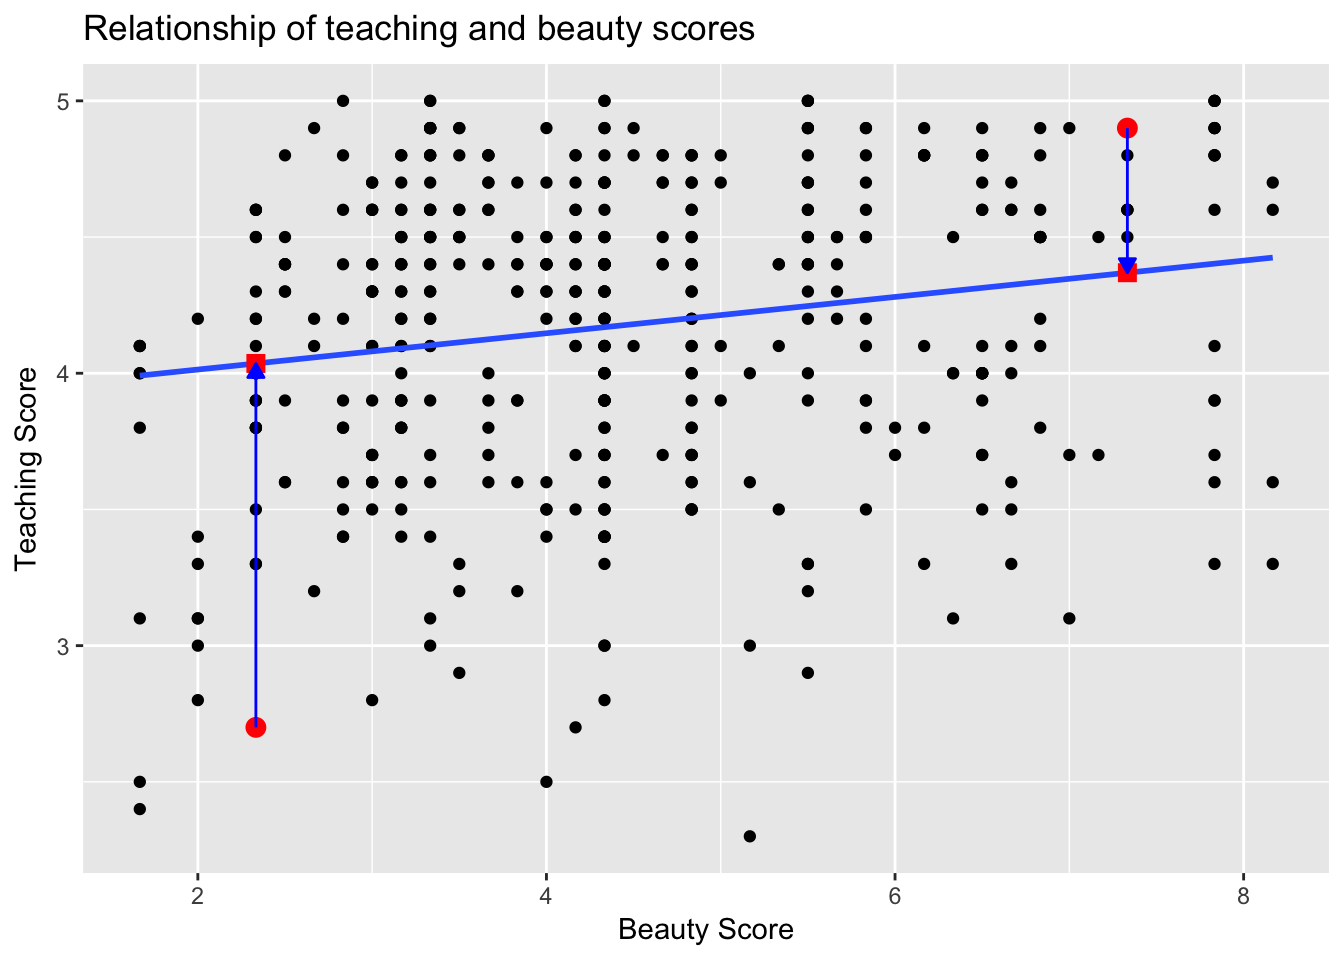
\includegraphics[width=\textwidth]{ismaykim_files/figure-latex/unnamed-chunk-64-1} 

}

\caption[Histogram of number of heads in simulation - needs tweaking]{Histogram of number of heads in simulation - needs tweaking}\label{fig:unnamed-chunk-64}
\end{figure}

This horizontal axis labels are a little confusing here. What does 2.5
or 7.5 heads mean? In \texttt{simGuesses}, \texttt{heads} is a
\texttt{numerical} variable. Thus, \texttt{ggplot} is expecting the
values to be on a continuous scale. We can switch the scale to be
discrete by invoking the \texttt{factor} function and using
\texttt{geom\_bar} instead of \texttt{geom\_histogram}:

\begin{Shaded}
\begin{Highlighting}[]
\KeywordTok{library}\NormalTok{(ggplot2)}
\NormalTok{simGuesses %>%}\StringTok{ }\KeywordTok{ggplot}\NormalTok{(}\KeywordTok{aes}\NormalTok{(}\DataTypeTok{x =} \KeywordTok{factor}\NormalTok{(heads))) +}
\StringTok{  }\KeywordTok{geom_bar}\NormalTok{()}
\end{Highlighting}
\end{Shaded}

\begin{figure}

{\centering 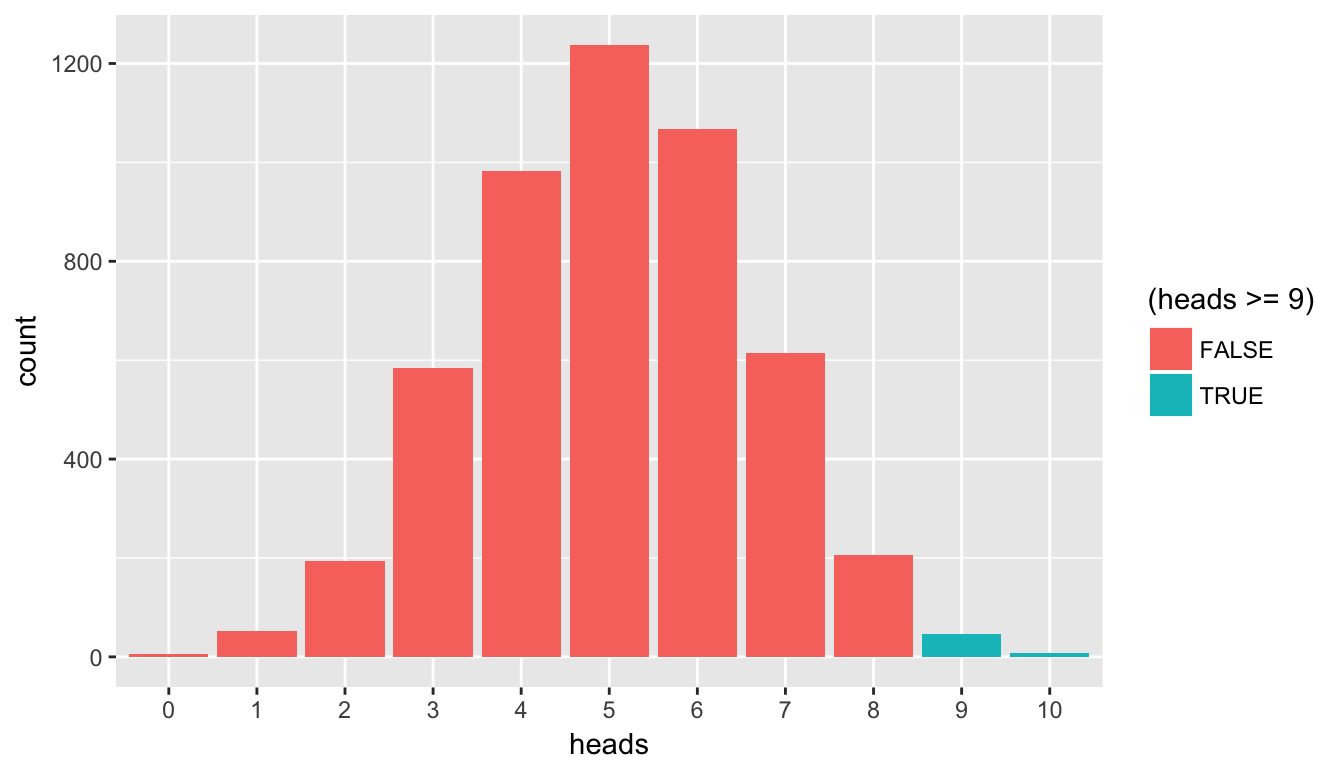
\includegraphics[width=\textwidth]{ismaykim_files/figure-latex/unnamed-chunk-65-1} 

}

\caption[Barplot of number of heads in simulation]{Barplot of number of heads in simulation}\label{fig:unnamed-chunk-65}
\end{figure}

You'll frequently need to make this conversion to \texttt{factor} when
making a barplot with quantitative variables. Remember from ``Getting
Used to R, RStudio, and R Markdown'' \citep{usedtor2016}, that a
\texttt{factor} variable is useful when there is a natural ordering to
the variable and it only takes on discrete values and not fractional
values like 2.5. Our \texttt{heads} variable has a natural ordering: 0,
1, 2, \(\ldots\), 10.

Again, note that the shape of these number of heads follows what appears
to be a normal distribution. We'll see that if appropriate
conditions/assumptions are met with the data that we can expect to see a
normal distribution result. When these conditions aren't met, the
simulation methodology we've presented here still works well whereas the
traditional normal-based methods start to fall apart.

We will delve further into hypothesis testing in the next few chapters.
This null distribution in combination with the \textbf{sampling
distribution} concept covered earlier will be of utmost importance going
forward.

\section{\texorpdfstring{Review of \texttt{mosaic} simulation
functions}{Review of mosaic simulation functions}}\label{review-of-mosaic-simulation-functions}

In this chapter, we've discussed three functions in the \texttt{mosaic}
package useful in understanding the stepping stones to statistical
inference: \texttt{do}, \texttt{rflip}, and \texttt{resample}. We will
also work with the \texttt{shuffle} function in later chapters and we
summarize it here for your reference later.

\begin{itemize}
\item
  \texttt{do}: Its main use is in replicating a process many times. It
  has one argument \texttt{n} which specifies how many times to
  replicate the process. It then uses \texttt{*}, which can be read as
  ``times'', and whatever follows immediately after it as the process.
\item
  \texttt{rflip}: This is used to simulate the flipping of a coin many
  times. By default, it flips a fair coin one time giving an equal
  chance to heads and tails. It is frequently used with \texttt{do()\ *}
  to simulate many coin flips in multiple sets.
\item
  \texttt{resample}: This is used to sample from a larger data set with
  or without replacement. When we are thinking about the concept of
  random sampling, we sample without replacement. We can also sample
  with replacement corresponding to the values being replaced into the
  pool to draw from with the possibility that they are drawn again in
  the resample. This will be of great importance when we discuss
  \textbf{bootstrapping} with confidence intervals.
\item
  \texttt{shuffle}: Its main purpose is to permute the values of one
  variable across the values of another variable. This acts in much the
  same way as shuffling a deck of cards and then presenting the shuffled
  deck to two (or more) players.
\end{itemize}

\begin{center}\rule{0.5\linewidth}{\linethickness}\end{center}

\begin{learncheck}
\textbf{\emph{Learning check}}
\end{learncheck}

\textbf{(LC6.16)} Recreate \texttt{rflip} using only the
\texttt{resample} function and specifying the appropriate arguments.

\textbf{(LC6.17)} Recreate \texttt{shuffle} using only the
\texttt{resample} function and specifying the appropriate arguments.

\begin{center}\rule{0.5\linewidth}{\linethickness}\end{center}

\section{Conclusion}\label{conclusion-2}

\subsection{Script of R code}\label{script-of-r-code-2}

An R script file of all R code used in this chapter is available
\href{http://ismayc.github.io/moderndiver-book/06-sim.R}{here}.

\subsection{What's to come?}\label{whats-to-come-3}

This chapter has served as an introduction into inferential techniques
that will be discussed in greater detail in Chapter \ref{hypo} for
hypothesis testing and in Chapter \ref{ci} for confidence intervals. In
these chapters, we will see how we can use a related concept of
\textbf{resampling} when working with the distributions of two groups.
All of these concepts will be further reinforced in Chapter
\ref{regress} as well.

\chapter{Hypothesis Testing}\label{hypo}

We saw some of the main concepts of hypothesis testing introduced in
Chapter \ref{sim}. We will expand further on these ideas here and also
provide a framework for understanding hypothesis tests in general.
Instead of presenting you with lots of different formulas and scenarios,
we hope to build a way to think about all hypothesis tests. You can then
adapt to different scenarios as needed down the road when you encounter
different statistical situations.

The same can be said for confidence intervals. There is one general
framework that applies to all confidence intervals and we will elaborate
on this further in Chapter \ref{ci}. The specifics may change slightly
for each variation, but the important idea is to understand the general
framework so that you can apply it to more specific problems. We believe
that this approach is much better in the long-term than teaching you
specific tests and confidence intervals rigorously. You can find full
worked out examples for five common hypothesis tests and their
corresponding confidence intervals in Appendix \ref{appendixB}. We
recommend that you carefully review these examples as they also cover
how the general frameworks apply to traditional normal-based
methodologies like the \(t\)-test and normal-theory confidence
intervals. You'll see there that these methods are just approximations
for the general computational frameworks, but require conditions to be
met for their results to be valid. The general frameworks using
randomization, simulation, and bootstrapping do not hold the same sorts
of restrictions and further advance computational thinking, which is one
big reason for their emphasis throughout this textbook.

\section*{Needed packages}\label{needed-packages-3}
\addcontentsline{toc}{section}{Needed packages}

\begin{Shaded}
\begin{Highlighting}[]
\KeywordTok{library}\NormalTok{(dplyr)}
\KeywordTok{library}\NormalTok{(ggplot2)}
\KeywordTok{library}\NormalTok{(okcupiddata)}
\KeywordTok{library}\NormalTok{(mosaic)}
\KeywordTok{library}\NormalTok{(knitr)}
\KeywordTok{library}\NormalTok{(nycflights13)}
\end{Highlighting}
\end{Shaded}

\section{When Inference Is Not
Needed}\label{when-inference-is-not-needed}

Before we delve into the two techniques of inference (hypothesis testing
and confidence intervals), it's good to remember that there are cases
where you need not perform a rigorous statistical inference. An
important and time-saving skill is to \textbf{ALWAYS} do exploratory
data analysis using \texttt{dplyr} and \texttt{ggplot2} before thinking
about running a hypothesis test. Let's look at such an example selecting
a sample of flights traveling to Boston and to San Francisco from New
York City in the \texttt{flights} data frame in the
\texttt{nycflights13} package. (We will remove flights with missing data
first using \texttt{na.omit} and then sample 100 flights going to each
of the two airports.)

\begin{Shaded}
\begin{Highlighting}[]
\KeywordTok{library}\NormalTok{(nycflights13)}
\KeywordTok{data}\NormalTok{(flights)}
\NormalTok{bos_sfo <-}\StringTok{ }\NormalTok{flights %>%}\StringTok{ }\KeywordTok{na.omit}\NormalTok{() %>%}\StringTok{ }
\StringTok{  }\KeywordTok{filter}\NormalTok{(dest %in%}\StringTok{ }\KeywordTok{c}\NormalTok{(}\StringTok{"BOS"}\NormalTok{, }\StringTok{"SFO"}\NormalTok{)) %>%}\StringTok{ }
\StringTok{  }\KeywordTok{group_by}\NormalTok{(dest) %>%}\StringTok{ }
\StringTok{  }\KeywordTok{sample_n}\NormalTok{(}\DecValTok{100}\NormalTok{)}
\end{Highlighting}
\end{Shaded}

Suppose we were interested in seeing if the \texttt{air\_time} to SFO in
San Francisco was statistically greater than the \texttt{air\_time} to
BOS in Boston. As suggested, let's begin with some exploratory data
analysis to get a sense for how the two variables of \texttt{air\_time}
and \texttt{dest} relate for these two destination airports:

\begin{Shaded}
\begin{Highlighting}[]
\KeywordTok{library}\NormalTok{(dplyr)}
\NormalTok{bos_sfo_summary <-}\StringTok{ }\NormalTok{bos_sfo %>%}\StringTok{ }\KeywordTok{group_by}\NormalTok{(dest) %>%}\StringTok{ }
\StringTok{  }\KeywordTok{summarize}\NormalTok{(}\DataTypeTok{mean_time =} \KeywordTok{mean}\NormalTok{(air_time),}
            \DataTypeTok{sd_time =} \KeywordTok{sd}\NormalTok{(air_time))}
\KeywordTok{kable}\NormalTok{(bos_sfo_summary)}
\end{Highlighting}
\end{Shaded}

\begin{tabular}{l|r|r}
\hline
dest & mean\_time & sd\_time\\
\hline
BOS & 38.35 & 5.726732\\
\hline
SFO & 345.61 & 15.354988\\
\hline
\end{tabular}

Looking at these results, we can clearly see that SFO \texttt{air\_time}
is much larger than BOS \texttt{air\_time}. The standard deviation is
also extremely informative here.

\begin{center}\rule{0.5\linewidth}{\linethickness}\end{center}

\begin{learncheck}
\textbf{\emph{Learning check}}
\end{learncheck}

\textbf{(LC7.1)} Could we make the same type of immediate conclusion
that SFO had a statistically greater \texttt{air\_time} if, say, its
corresponding standard deviation was 200 minutes? What about 100
minutes? Explain.

\begin{center}\rule{0.5\linewidth}{\linethickness}\end{center}

To further understand just how different the \texttt{air\_time} variable
is for BOS and SFO, let's look at a boxplot:

\begin{Shaded}
\begin{Highlighting}[]
\KeywordTok{library}\NormalTok{(ggplot2)}
\KeywordTok{ggplot}\NormalTok{(}\DataTypeTok{data =} \NormalTok{bos_sfo, }\DataTypeTok{mapping =} \KeywordTok{aes}\NormalTok{(}\DataTypeTok{x =} \NormalTok{dest, }\DataTypeTok{y =} \NormalTok{air_time)) +}
\StringTok{  }\KeywordTok{geom_boxplot}\NormalTok{()}
\end{Highlighting}
\end{Shaded}

\begin{center}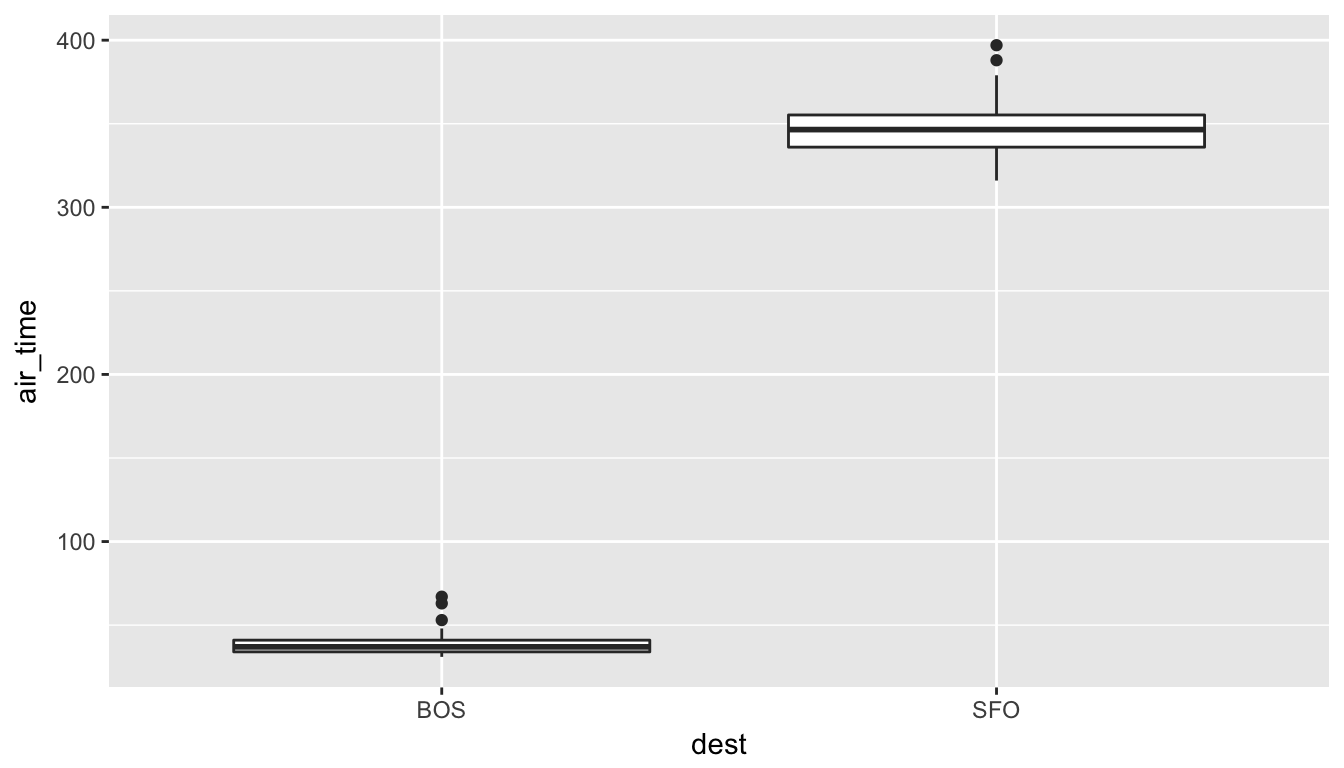
\includegraphics[width=\textwidth]{ismaykim_files/figure-latex/unnamed-chunk-70-1} \end{center}

Since there is no overlap at all, we can conclude that the
\texttt{air\_time} for San Francisco flights is statistically greater
(at any level of significance) than the \texttt{air\_time} for Boston
flights. This is a clear example of not needing to do anything more than
some simple descriptive statistics to get an appropriate inferential
conclusion. This is one reason why you should \textbf{ALWAYS}
investigate the sample data first using \texttt{dplyr} and
\texttt{ggplot2} via exploratory data analysis.

As you get more and more practice with hypothesis testing, you'll be
better able to determine in many cases whether or not the results will
be statistically significant. There are circumstances where it is
difficult to tell, but you should always try to make a guess FIRST about
significance after you have completed your data exploration and before
you actually begin the inferential techniques.

\section{Basics of Hypothesis
Testing}\label{basics-of-hypothesis-testing}

In a hypothesis test, we will use data from a sample to help us decide
between two competing \emph{hypotheses} about a population. We make
these hypotheses more concrete by specifying them in terms of at least
one \emph{population parameter} of interest. We refer to the competing
claims about the population as the \textbf{null hypothesis}, denoted by
\(H_0\), and the \textbf{alternative (or research) hypothesis}, denoted
by \(H_a\). The roles of these two hypotheses are NOT interchangeable.

\begin{itemize}
\tightlist
\item
  The claim for which we seek significant evidence is assigned to the
  alternative hypothesis. The alternative is usually what the
  experimenter or researcher wants to establish or find evidence for.
\item
  Usually, the null hypothesis is a claim that there really is ``no
  effect'' or ``no difference.'' In many cases, the null hypothesis
  represents the status quo or that nothing interesting is happening.\\
\item
  We assess the strength of evidence by assuming the null hypothesis is
  true and determining how unlikely it would be to see sample
  results/statistics as extreme (or more extreme) as those in the
  original sample.
\end{itemize}

Hypothesis testing brings about many weird and incorrect notions in the
scientific community and society at large. One reason for this is that
statistics has traditionally been thought of as this magic box of
algorithms and procedures to get to results and this has been readily
apparent if you do a Google search of ``flowchart statistics hypothesis
tests''. There are so many different complex ways to determine which
test is appropriate.

You'll see that we don't need to rely on these complicated series of
assumptions and procedures to conduct a hypothesis test any longer.
These methods were introduced in a time when computers weren't powerful.
Your cellphone (in 2016) has more power than the computers that sent
NASA astronauts to the moon after all. We'll see that ALL hypothesis
tests can be broken down into the following framework given by Allen
Downey
\href{http://allendowney.blogspot.com/2016/06/there-is-still-only-one-test.html}{here}:

\begin{figure}

{\centering 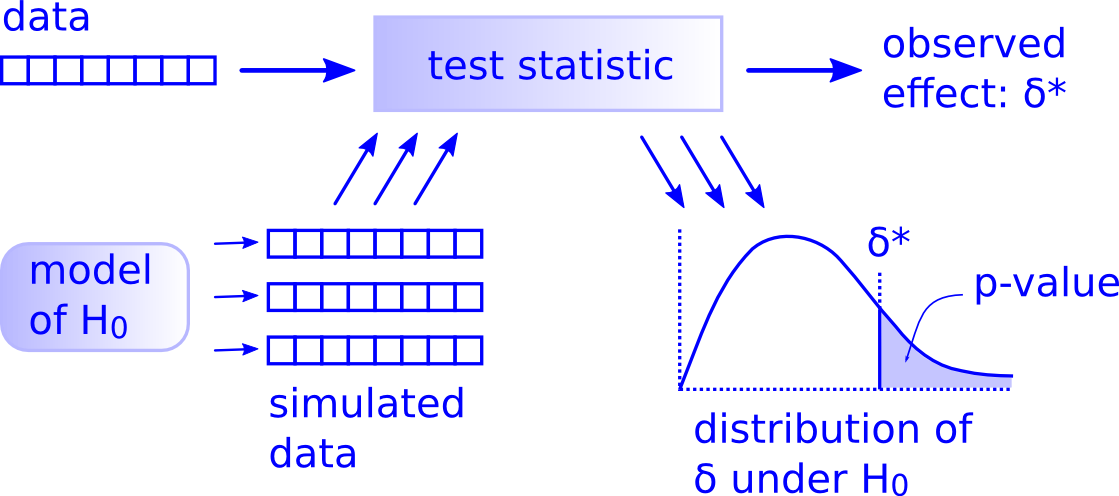
\includegraphics[width=\textwidth]{images/ht} 

}

\caption[Hypothesis Testing Framework]{Hypothesis Testing Framework}\label{fig:htdowney}
\end{figure}

Before we hop into this framework, we will provide another way to think
about hypothesis testing that may be useful.

\section{Criminal trial analogy}\label{trial}

We can think of hypothesis testing in the same context as a criminal
trial in the United States. A criminal trial in the United States is a
familiar situation in which a choice between two contradictory claims
must be made. 1. The accuser of the crime must be judged either guilty
or not guilty.

\begin{enumerate}
\def\labelenumi{\arabic{enumi}.}
\setcounter{enumi}{1}
\item
  Under the U.S. system of justice, the individual on trial is initially
  presumed not guilty.
\item
  Only STRONG EVIDENCE to the contrary causes the not guilty claim to be
  rejected in favor of a guilty verdict.
\item
  The phrase ``beyond a reasonable doubt'' is often used to set the
  cutoff value for when enough evidence has been given to convict.
\end{enumerate}

Theoretically, we should never say ``The person is innocent.'' but
instead ``There is not sufficient evidence to show that the person is
guilty.''

Now let's compare that to how we look at a hypothesis test.

\begin{enumerate}
\def\labelenumi{\arabic{enumi}.}
\item
  The decision about the population parameter(s) must be judged to
  follow one of two hypotheses.
\item
  We initially assume that \(H_0\) is true.
\item
  The null hypothesis \(H_0\) will be rejected (in favor of \(H_a\))
  only if the sample evidence strongly suggests that \(H_0\) is false.
  If the sample does not provide such evidence, \(H_0\) will not be
  rejected.
\item
  The analogy to ``beyond a reasonable doubt'' in hypothesis testing is
  what is known as the \textbf{significance level}. This will be set
  before conducting the hypothesis test and is denoted as \(\alpha\).
  Common values for \(\alpha\) are 0.1, 0.01, and 0.05.
\end{enumerate}

\subsection{Two possible conclusions}\label{two-possible-conclusions}

Therefore, we have two possible conclusions with hypothesis testing:

\begin{itemize}
\tightlist
\item
  Reject \(H_0\)\\
\item
  Fail to reject \(H_0\)
\end{itemize}

Gut instinct says that ``Fail to reject \(H_0\)'' should say ``Accept
\(H_0\)'' but this technically is not correct. Accepting \(H_0\) is the
same as saying that a person is innocent. We cannot show that a person
is innocent; we can only say that there was not enough substantial
evidence to find the person guilty.

When you run a hypothesis test, you are the jury of the trial. You
decide whether there is enough evidence to convince yourself that
\(H_a\) is true (``the person is guilty'') or that there was not enough
evidence to convince yourself \(H_a\) is true (``the person is not
guilty''). You must convince yourself (using statistical arguments)
which hypothesis is the correct one given the sample information.

\textbf{Important note:} Therefore, DO NOT WRITE ``Accept \(H_0\)'' any
time you conduct a hypothesis test. Instead write ``Fail to reject
\(H_0\).''

\section{Types of Errors in Hypothesis
Testing}\label{types-of-errors-in-hypothesis-testing}

Unfortunately, just as a jury or a judge can make an incorrect decision
in regards to a criminal trial by reaching the wrong verdict, there is
some chance we will reach the wrong conclusion via a hypothesis test
about a population parameter. As with criminal trials, this comes from
the fact that we don't have complete information, but rather a sample
from which to try to infer about a population.

The possible erroneous conclusions in a criminal trial are

\begin{itemize}
\tightlist
\item
  an innocent person is convicted (found guilty) or
\item
  a guilty person is set free (found not guilty).
\end{itemize}

The possible errors in a hypothesis test are - rejecting \(H_0\) when in
fact \(H_0\) is true (Type I Error) - failing to reject \(H_0\) when in
fact \(H_0\) is false (Type II Error)

The risk of error is the price researchers pay for basing an inference
about a population on a sample. With any reasonable sample-based
procedure, there is some chance that a Type I error will be made and
some chance that a Type II error will occur.

To help understand the concepts of Type I error and Type II error,
observe the following table:

\begin{figure}

{\centering 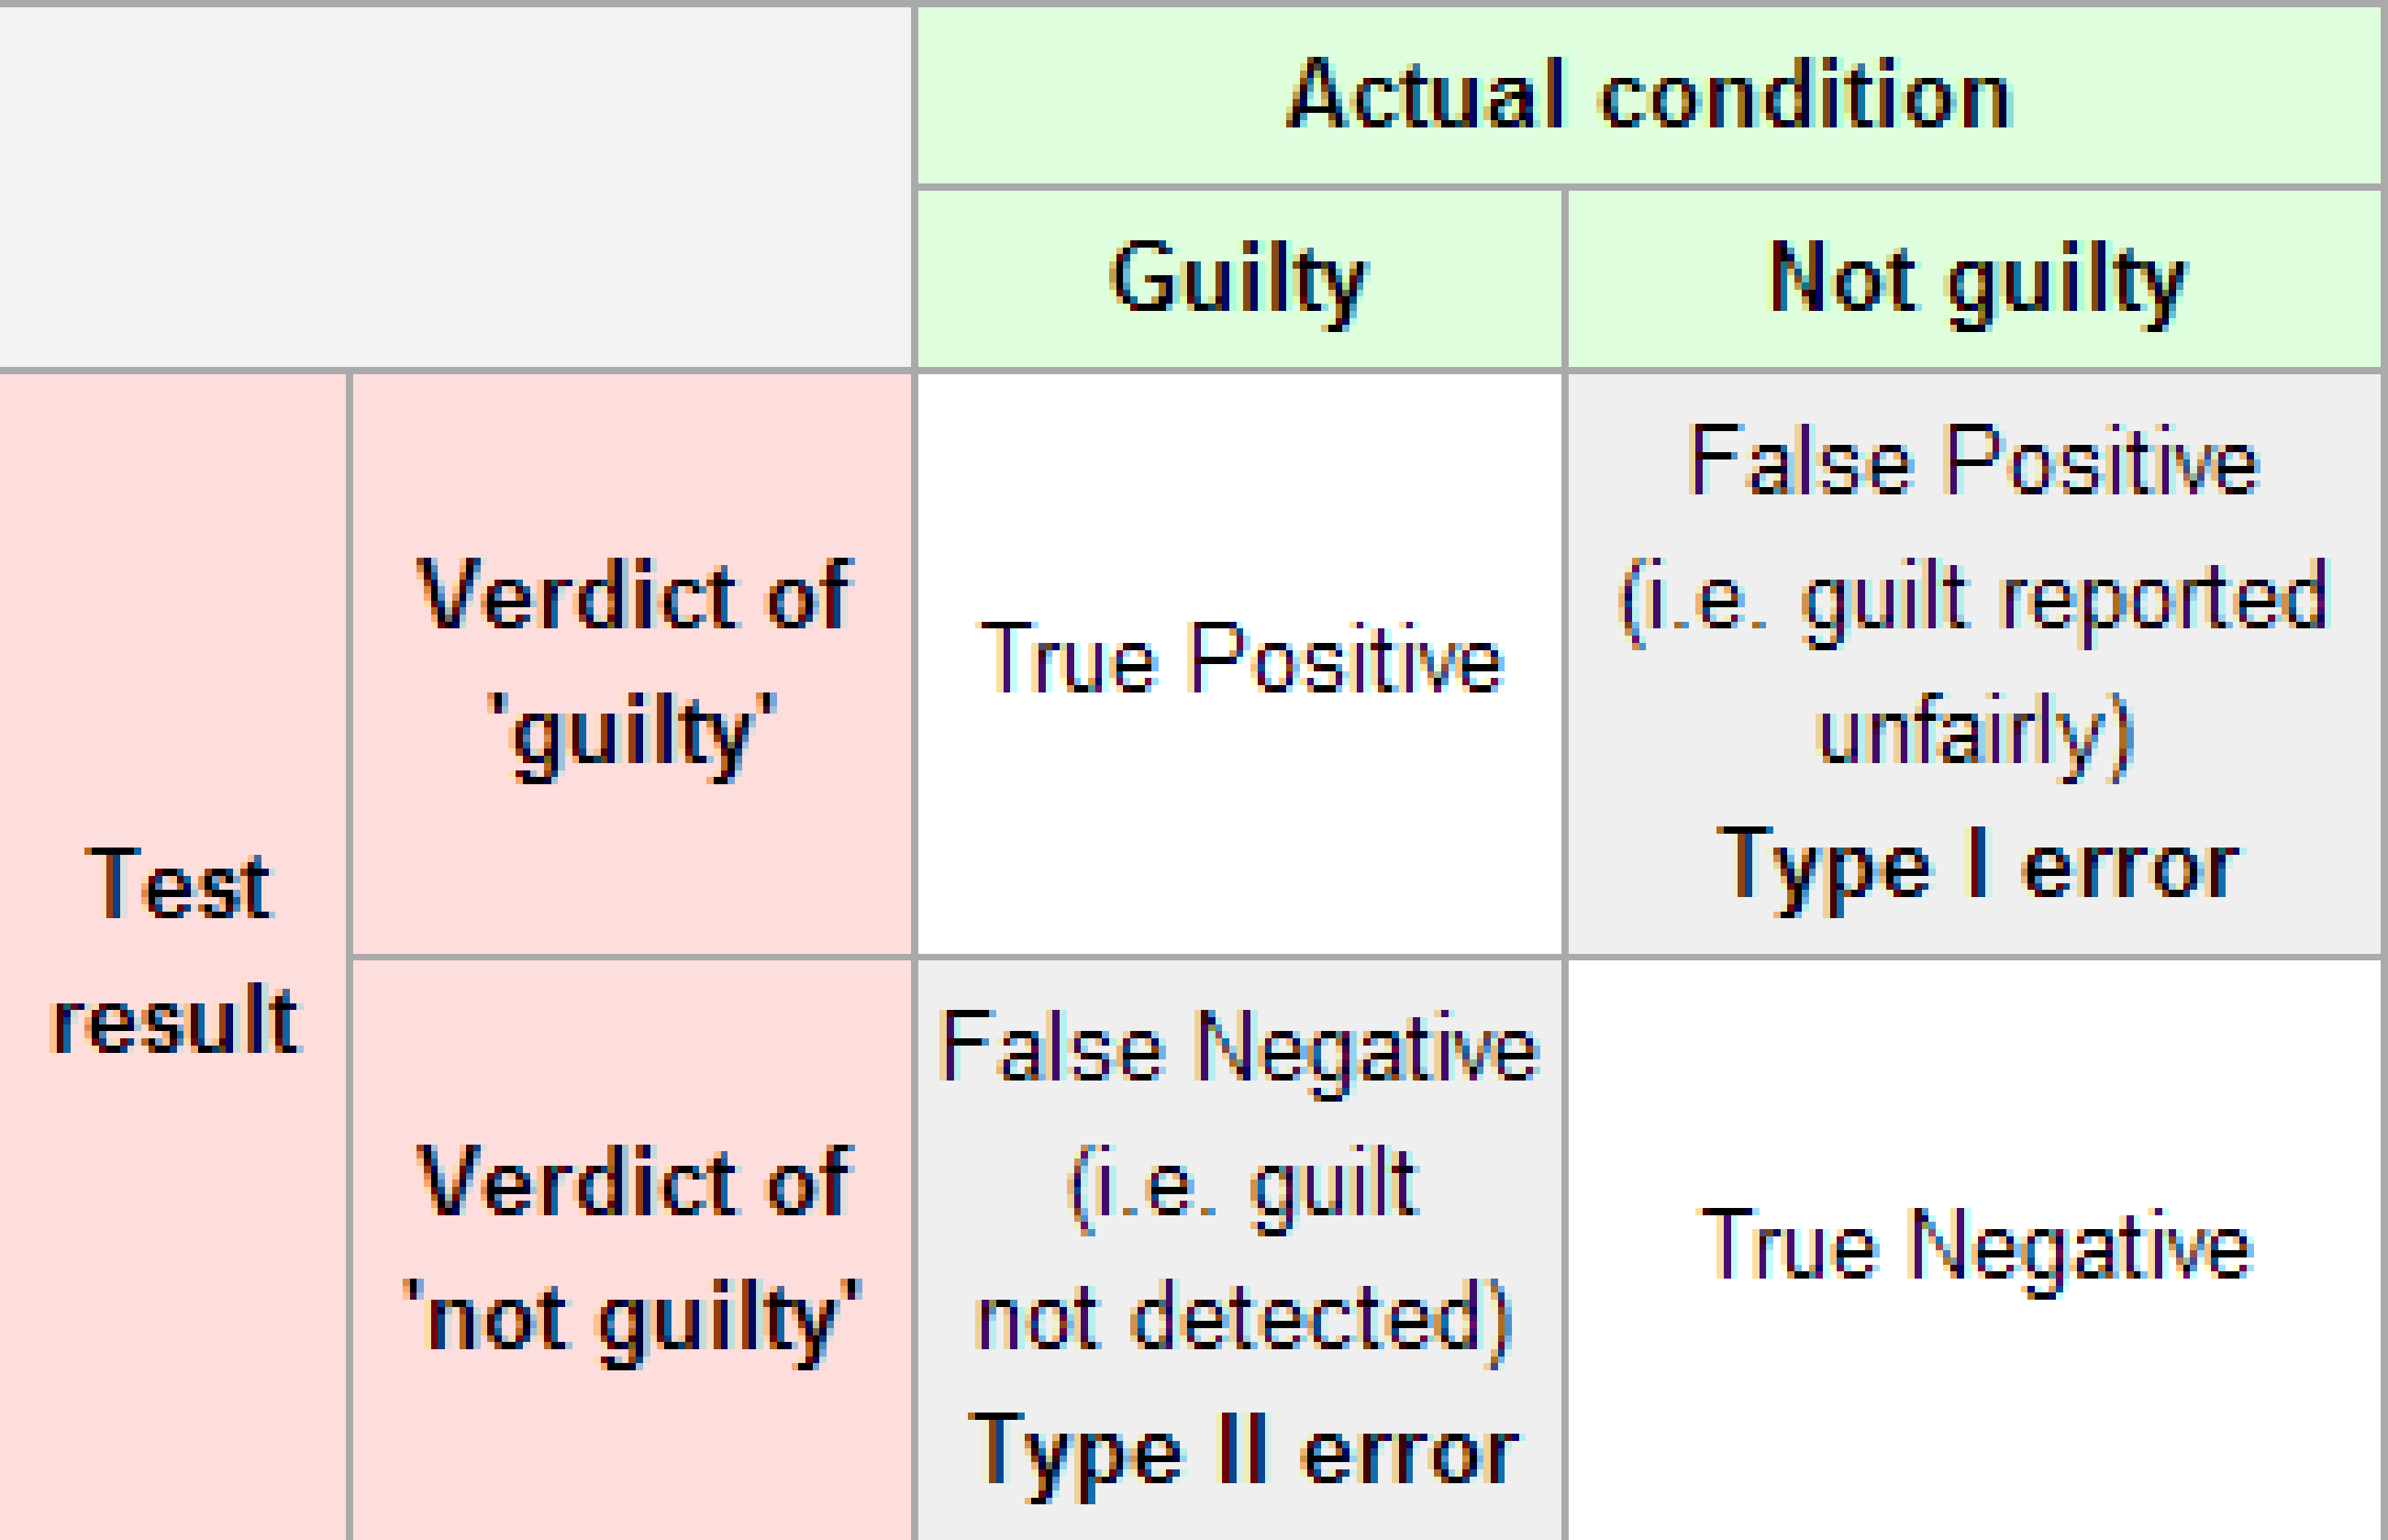
\includegraphics[width=\textwidth]{images/errors} 

}

\caption[Type I and Type II errors]{Type I and Type II errors}\label{fig:unnamed-chunk-71}
\end{figure}

If we are using sample data to make inferences about a parameter, we run
the risk of making a mistake. Obviously, we want to minimize our chance
of error; we want a small probability of drawing an incorrect
conclusion.

\begin{itemize}
\tightlist
\item
  The probability of a Type I Error occurring is denoted by \(\alpha\)
  and is called the \textbf{significance level} of a hypothesis test
\item
  The probability of a Type II Error is denoted by \(\beta\).
\end{itemize}

Formally, we can define \(\alpha\) and \(\beta\) in regards to the table
above, but for hypothesis tests instead of a criminal trial.

\begin{itemize}
\tightlist
\item
  \(\alpha\) corresponds to the probability of rejecting \(H_0\) when,
  in fact, \(H_0\) is true.
\item
  \(\beta\) corresponds to the probability of failing to reject \(H_0\)
  when, in fact, \(H_0\) is false.
\end{itemize}

Ideally, we want \(\alpha = 0\) and \(\beta = 0\), meaning that the
chance of making an error does not exist. When we have to use incomplete
information (sample data), it is not possible to have both
\(\alpha = 0\) and \(\beta = 0\). We will always have the possibility of
at least one error existing when we use sample data.

Usually, what is done is that \(\alpha\) is set before the hypothesis
test is conducted and then the evidence is judged against that
significance level. Common values for \(\alpha\) are 0.05, 0.01, and
0.10. If \(\alpha = 0.05\), we are using a testing procedure that, used
over and over with different samples, rejects a TRUE null hypothesis
five percent of the time.

So if we can set \(\alpha\) to be whatever we want, why choose 0.05
instead of 0.01 or even better 0.0000000000000001? Well, a small
\(\alpha\) means the test procedure requires the evidence against
\(H_0\) to be \textbf{very strong} before we can reject \(H_0\). This
means we will almost never reject \(H_0\) if \(\alpha\) is very small.
If we almost never reject \(H_0\), the probability of a Type II Error --
failing to reject \(H_0\) when we should -- will \emph{increase}! Thus,
as \(\alpha\) decreases, \(\beta\) increases and as \(\alpha\)
increases, \(\beta\) decreases. We, therefore, need to strike a balance
in \(\alpha\) and \(\beta\) and the common values of 0.05, 0.01, and
0.10 usually lead to a nice balance.

\begin{center}\rule{0.5\linewidth}{\linethickness}\end{center}

\begin{learncheck}
\textbf{\emph{Learning check}}
\end{learncheck}

\textbf{(LC7.2)} Reproduce the table above, but for a hypothesis test,
instead of the one provided for a criminal trial.

\begin{center}\rule{0.5\linewidth}{\linethickness}\end{center}

\subsection{Logic of Hypothesis
Testing}\label{logic-of-hypothesis-testing}

\begin{itemize}
\tightlist
\item
  Take a random sample (or samples) from a population (or two
  populations)
\item
  If the sample data are consistent with the null hypothesis, do not
  reject the null hypothesis.
\item
  If the sample data are inconsistent with the null hypothesis (in the
  direction of the alternative hypothesis), reject the null hypothesis
  and conclude that there is evidence the alternative hypothesis is true
  (based on the particular sample collected).
\end{itemize}

\section{Statistical Significance}\label{statistical-significance}

The idea that sample results are more extreme than we would reasonably
expect to see by random chance if the null hypothesis were true is the
fundamental idea behind statistical hypothesis tests. If data as extreme
would be very unlikely if the null hypothesis were true, we say the data
are \textbf{statistically significant}. Statistically significant data
provide convincing evidence against the null hypothesis in favor of the
alternative, and allow us to generalize our sample results to the claim
about the population.

\begin{center}\rule{0.5\linewidth}{\linethickness}\end{center}

\textbf{Definition: Statistical Significance}

When results as extreme as the observed sample statistic are unlikely to
occur by random chance alone (assuming the null hypothesis is true), we
say the sample results/statistics are \emph{statistically significant}.
If our sample is statistically significant, we have convincing evidence
against \(H_0\) and in favor of \(H_a\).

\begin{center}\rule{0.5\linewidth}{\linethickness}\end{center}

\begin{learncheck}
\textbf{\emph{Learning check}}
\end{learncheck}

\textbf{(LC7.3)} What is wrong about saying ``The defendant is
innocent.'' based on the US system of criminal trials?

\textbf{(LC7.4)} What is the purpose of hypothesis testing?

\textbf{(LC7.5)} What are some flaws with hypothesis testing? How could
we alleviate them?

\begin{center}\rule{0.5\linewidth}{\linethickness}\end{center}

\section{EXAMPLE: Revisiting the Lady Tasting
Tea}\label{example-revisiting-the-lady-tasting-tea}

Recall the ``There is Only One Test'' diagram from earlier:

\begin{figure}

{\centering 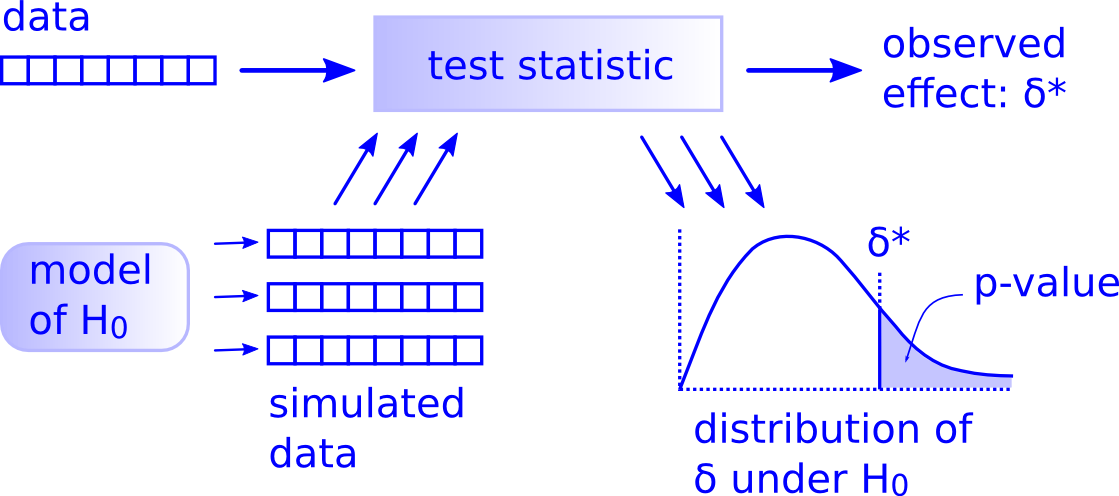
\includegraphics[width=\textwidth]{images/ht} 

}

\caption[Hypothesis Testing Framework]{Hypothesis Testing Framework}\label{fig:htdowney2}
\end{figure}

We will now walk-through how each of the steps to the diagram apply to
determining whether the lady tasting tea was actually better than chance
at determining whether or not milk was added first. We will see that the
process of creating a null distribution is a statistical way to
quantifying surprise.

\subsection{Data}\label{data}

Let's assume as we did in Chapter \ref{sim}, that the lady is correct in
determining whether milk was added first or not in 9 out of 10 trials.
Our data, therefore, may look something like

\begin{tabular}{l}
\hline
Correct\\
\hline
Correct\\
\hline
Correct\\
\hline
Incorrect\\
\hline
Correct\\
\hline
Correct\\
\hline
Correct\\
\hline
Correct\\
\hline
Correct\\
\hline
Correct\\
\hline
\end{tabular}

\subsection{\texorpdfstring{Test Statistic
\(\delta\)}{Test Statistic \textbackslash{}delta}}\label{test-statistic-delta}

We are interested in the number of \texttt{Correct} out of our 10
trials. We can denote this number of successes using the symbol \(t\),
where \(t\) corresponds to total. This is our test statistic \(\delta\)
in this case.

\subsection{\texorpdfstring{Observed effect
\(\delta^*\)}{Observed effect \textbackslash{}delta\^{}*}}\label{observed-effect-delta}

The actual observed value of the test statistic from our observed sample
is \(\hat{t}_{obs} = 9\). Thus, \(\delta^* = 9\).

\subsection{\texorpdfstring{Model of
\(H_0\)}{Model of H\_0}}\label{model-of-h_0}

Our null hypothesis is that the lady is only as good as chance at
guessing correctly. Hypotheses always correspond to parameters and are
denoted with Greek letters. Thus, symbolically, we have
\(H_0: \tau = 5\). Since we are assuming chance and we have 10 flips
with 0.5 probability of success of each flip, we have
\(\tau = 10 \times 0.5 = 5\).

\subsection{Simulated Data}\label{simulated-data}

We now want to use this null hypothesis to simulate the test statistic
assuming that the null hypothesis is true. Therefore, we want to figure
out a way to simulate in 10 trials, getting either the choice Correct or
Incorrect, assuming that the probability of success (getting it Correct)
in any given trial is 0.5.

\textbf{Tactile simulation}

When you are presented with a hypothesis testing problem, frequently the
most challenging portion is setting up how to simulate the data assuming
the null hypothesis is true. To facilitate with this, setting up a
tactile, hands on experiment can help.

In this case, flipping a fair coin is a great way to simulate this
process. To simulate 10 trials, we could flip the fair coin and record
Heads as Correct and Tails as Incorrect.

Some simulated data using this coin flipping procedure may look like the
following. Note that this data frame is not tidy, but is a convenient
way to look at the results of the simulation in this wide format. The
numbers on the fair left correspond to the number of the trial.

\begin{tabular}{l|l|l|l}
\hline
  & sample1 & sample2 & sample3\\
\hline
1 & Correct & Correct & Correct\\
\hline
2 & Correct & Incorrect & Incorrect\\
\hline
3 & Incorrect & Incorrect & Correct\\
\hline
4 & Incorrect & Incorrect & Correct\\
\hline
5 & Correct & Incorrect & Incorrect\\
\hline
6 & Correct & Incorrect & Correct\\
\hline
7 & Incorrect & Incorrect & Correct\\
\hline
8 & Incorrect & Correct & Incorrect\\
\hline
9 & Incorrect & Correct & Incorrect\\
\hline
10 & Incorrect & Correct & Incorrect\\
\hline
\end{tabular}

We then use the formula for the \textbf{Test Statistic} to determine the
simulated test statistic for each of these simulated samples. So in this
case we have

\(t_1 = 4\), \(t_2 = 4\), \(t_3 = 5\)

\subsection{\texorpdfstring{Distribution of \(\delta\) under
\(H_0\)}{Distribution of \textbackslash{}delta under H\_0}}\label{distribution-of-delta-under-h_0}

We could continue this process say 10,000 times by flipping a coin in
sets of 10 for 10,000 repetitions and counting and taking note of how
many heads out of 10 we have for each set. It's at this point that you
realize that a computer can do this procedure much faster and more
efficient than the tactile experiment with a coin.

Recall that we've already created the distribution of 10,000 such coin
flips and we've stored these values in the \texttt{heads} variable in
the \texttt{simGuesses} data frame:

\begin{Shaded}
\begin{Highlighting}[]
\KeywordTok{library}\NormalTok{(ggplot2)}
\KeywordTok{ggplot}\NormalTok{(}\DataTypeTok{data =} \NormalTok{simGuesses, }\KeywordTok{aes}\NormalTok{(}\DataTypeTok{x =} \KeywordTok{factor}\NormalTok{(heads))) +}
\StringTok{  }\KeywordTok{geom_bar}\NormalTok{()}
\end{Highlighting}
\end{Shaded}

\begin{center}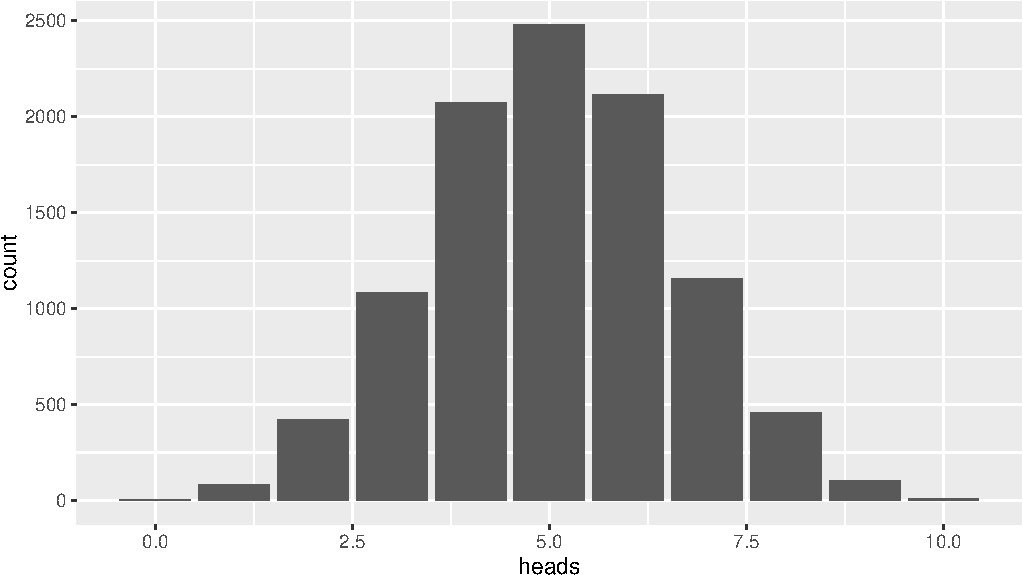
\includegraphics[width=\textwidth]{ismaykim_files/figure-latex/unnamed-chunk-75-1} \end{center}

\subsection{The p-value}\label{the-p-value}

\begin{center}\rule{0.5\linewidth}{\linethickness}\end{center}

\textbf{Definition: \(p\)-value}:

The \textbf{p-value} is the probability of observing a sample statistic
as extreme or more extreme than what was observed, assuming that the
null hypothesis of a by chance operation is true.

\begin{center}\rule{0.5\linewidth}{\linethickness}\end{center}

This definition may be a little intimidating the first time you read it,
but it's important to come back to this ``The Lady Tasting Tea'' problem
whenever you encounter \(p\)-values as you begin to learn about the
concept. Here the \(p\)-value corresponds to how many times in our
\textbf{null distribution} of \texttt{heads} 9 or more heads occurred.

We can use another neat feature of R to calculate the \(p\)-value for
this problem. Note that ``more extreme'' in this case corresponds to
looking at values of 9 or greater since our alternative hypothesis
invokes a right-tail test corresponding to a ``greater than'' hypothesis
of \(H_a: \pi > 0.5\). In other words, we are looking to see how likely
it is for the lady to pick 9 or more correct instead of 9 or less
correct. We'd like to go in the right direction.

\begin{Shaded}
\begin{Highlighting}[]
\NormalTok{pvalue_tea <-}\StringTok{ }\NormalTok{simGuesses %>%}
\StringTok{  }\KeywordTok{filter}\NormalTok{(heads >=}\StringTok{ }\DecValTok{9}\NormalTok{) %>%}
\StringTok{  }\KeywordTok{nrow}\NormalTok{() /}\StringTok{ }\KeywordTok{nrow}\NormalTok{(simGuesses)}
\end{Highlighting}
\end{Shaded}

Let's walk through each step of this calculation:

\begin{enumerate}
\def\labelenumi{\arabic{enumi}.}
\item
  First, \texttt{pvalue\_tea} will be the name of our calculated
  \(p\)-value and the assignment operator \texttt{\textless{}-} directs
  us to this naming.
\item
  We are working with the \texttt{simGuesses} data frame here so that
  comes immediately before the pipe operator.
\item
  We would like to only focus on the rows in our \texttt{simGuesses}
  data frame that have \texttt{heads} values of 9 or 10. This represents
  simulated statistics ``as extreme or more extreme'' than what we
  observed (9 correct guesses out of 10). Let's get a glimpse of what we
  have up to this point:

\begin{Shaded}
\begin{Highlighting}[]
\KeywordTok{kable}\NormalTok{(simGuesses %>%}\StringTok{ }\KeywordTok{filter}\NormalTok{(heads >=}\StringTok{ }\DecValTok{9}\NormalTok{))    }
\end{Highlighting}
\end{Shaded}

  \begin{tabular}{r|r|r|r}
  \hline
  n & heads & tails & prop\\
  \hline
  10 & 9 & 1 & 0.9\\
  \hline
  10 & 10 & 0 & 1.0\\
  \hline
  10 & 9 & 1 & 0.9\\
  \hline
  10 & 9 & 1 & 0.9\\
  \hline
  10 & 10 & 0 & 1.0\\
  \hline
  10 & 9 & 1 & 0.9\\
  \hline
  10 & 9 & 1 & 0.9\\
  \hline
  10 & 9 & 1 & 0.9\\
  \hline
  10 & 9 & 1 & 0.9\\
  \hline
  10 & 9 & 1 & 0.9\\
  \hline
  10 & 9 & 1 & 0.9\\
  \hline
  10 & 9 & 1 & 0.9\\
  \hline
  10 & 9 & 1 & 0.9\\
  \hline
  10 & 9 & 1 & 0.9\\
  \hline
  10 & 9 & 1 & 0.9\\
  \hline
  10 & 9 & 1 & 0.9\\
  \hline
  10 & 9 & 1 & 0.9\\
  \hline
  10 & 9 & 1 & 0.9\\
  \hline
  10 & 9 & 1 & 0.9\\
  \hline
  10 & 9 & 1 & 0.9\\
  \hline
  10 & 9 & 1 & 0.9\\
  \hline
  10 & 9 & 1 & 0.9\\
  \hline
  10 & 10 & 0 & 1.0\\
  \hline
  10 & 10 & 0 & 1.0\\
  \hline
  10 & 10 & 0 & 1.0\\
  \hline
  10 & 9 & 1 & 0.9\\
  \hline
  10 & 9 & 1 & 0.9\\
  \hline
  10 & 9 & 1 & 0.9\\
  \hline
  10 & 9 & 1 & 0.9\\
  \hline
  10 & 9 & 1 & 0.9\\
  \hline
  10 & 9 & 1 & 0.9\\
  \hline
  10 & 9 & 1 & 0.9\\
  \hline
  10 & 10 & 0 & 1.0\\
  \hline
  10 & 9 & 1 & 0.9\\
  \hline
  10 & 9 & 1 & 0.9\\
  \hline
  10 & 10 & 0 & 1.0\\
  \hline
  10 & 9 & 1 & 0.9\\
  \hline
  10 & 9 & 1 & 0.9\\
  \hline
  10 & 9 & 1 & 0.9\\
  \hline
  10 & 9 & 1 & 0.9\\
  \hline
  10 & 9 & 1 & 0.9\\
  \hline
  10 & 9 & 1 & 0.9\\
  \hline
  10 & 9 & 1 & 0.9\\
  \hline
  10 & 9 & 1 & 0.9\\
  \hline
  10 & 9 & 1 & 0.9\\
  \hline
  10 & 9 & 1 & 0.9\\
  \hline
  10 & 9 & 1 & 0.9\\
  \hline
  10 & 9 & 1 & 0.9\\
  \hline
  10 & 9 & 1 & 0.9\\
  \hline
  10 & 9 & 1 & 0.9\\
  \hline
  10 & 9 & 1 & 0.9\\
  \hline
  10 & 9 & 1 & 0.9\\
  \hline
  10 & 9 & 1 & 0.9\\
  \hline
  10 & 9 & 1 & 0.9\\
  \hline
  10 & 9 & 1 & 0.9\\
  \hline
  10 & 10 & 0 & 1.0\\
  \hline
  10 & 10 & 0 & 1.0\\
  \hline
  10 & 9 & 1 & 0.9\\
  \hline
  10 & 9 & 1 & 0.9\\
  \hline
  10 & 9 & 1 & 0.9\\
  \hline
  10 & 9 & 1 & 0.9\\
  \hline
  10 & 9 & 1 & 0.9\\
  \hline
  10 & 9 & 1 & 0.9\\
  \hline
  10 & 9 & 1 & 0.9\\
  \hline
  10 & 9 & 1 & 0.9\\
  \hline
  10 & 10 & 0 & 1.0\\
  \hline
  10 & 9 & 1 & 0.9\\
  \hline
  10 & 9 & 1 & 0.9\\
  \hline
  10 & 9 & 1 & 0.9\\
  \hline
  10 & 9 & 1 & 0.9\\
  \hline
  10 & 9 & 1 & 0.9\\
  \hline
  10 & 9 & 1 & 0.9\\
  \hline
  10 & 9 & 1 & 0.9\\
  \hline
  10 & 9 & 1 & 0.9\\
  \hline
  10 & 9 & 1 & 0.9\\
  \hline
  10 & 9 & 1 & 0.9\\
  \hline
  10 & 9 & 1 & 0.9\\
  \hline
  10 & 9 & 1 & 0.9\\
  \hline
  10 & 10 & 0 & 1.0\\
  \hline
  10 & 9 & 1 & 0.9\\
  \hline
  10 & 9 & 1 & 0.9\\
  \hline
  10 & 10 & 0 & 1.0\\
  \hline
  10 & 9 & 1 & 0.9\\
  \hline
  10 & 9 & 1 & 0.9\\
  \hline
  10 & 9 & 1 & 0.9\\
  \hline
  10 & 10 & 0 & 1.0\\
  \hline
  10 & 10 & 0 & 1.0\\
  \hline
  10 & 9 & 1 & 0.9\\
  \hline
  10 & 9 & 1 & 0.9\\
  \hline
  10 & 9 & 1 & 0.9\\
  \hline
  10 & 9 & 1 & 0.9\\
  \hline
  10 & 9 & 1 & 0.9\\
  \hline
  10 & 9 & 1 & 0.9\\
  \hline
  10 & 9 & 1 & 0.9\\
  \hline
  10 & 9 & 1 & 0.9\\
  \hline
  10 & 9 & 1 & 0.9\\
  \hline
  10 & 9 & 1 & 0.9\\
  \hline
  10 & 9 & 1 & 0.9\\
  \hline
  10 & 9 & 1 & 0.9\\
  \hline
  10 & 9 & 1 & 0.9\\
  \hline
  10 & 9 & 1 & 0.9\\
  \hline
  10 & 9 & 1 & 0.9\\
  \hline
  10 & 9 & 1 & 0.9\\
  \hline
  10 & 9 & 1 & 0.9\\
  \hline
  10 & 9 & 1 & 0.9\\
  \hline
  \end{tabular}
\item
  Now that we have changed the focus to only those rows that have number
  of heads out of 10 flips corresponding to 9 or more, we count how many
  of those there are. The function \texttt{nrow} gives how many entries
  are in this filtered data frame and lastly we calculate the proportion
  that are at least as extreme as our observed value of 9 by dividing by
  the number of total simulations (10,000).
\end{enumerate}

We can see that the observed statistic of 9 correct guesses is not a
likely outcome assuming the null hypothesis is true. Only around 1\% of
the outcomes in our 10,000 simulations fall at or above 9 successes. We
have evidence supporting the conclusion that the person is actually
better than just guessing at random at determining whether milk has been
added first or not. To better visualize this we can also make use of
pink shading on the histogram corresponding to the \(p\)-value:

\begin{Shaded}
\begin{Highlighting}[]
\KeywordTok{library}\NormalTok{(ggplot2)}
  \KeywordTok{ggplot}\NormalTok{(}\DataTypeTok{data =} \NormalTok{simGuesses, }\KeywordTok{aes}\NormalTok{(}\DataTypeTok{x =} \KeywordTok{factor}\NormalTok{(heads), }\DataTypeTok{fill =} \NormalTok{(heads >=}\StringTok{ }\DecValTok{9}\NormalTok{))) +}
\StringTok{  }\KeywordTok{geom_bar}\NormalTok{() +}
\StringTok{  }\KeywordTok{labs}\NormalTok{(}\DataTypeTok{x =} \StringTok{"heads"}\NormalTok{)}
\end{Highlighting}
\end{Shaded}

\begin{figure}

{\centering 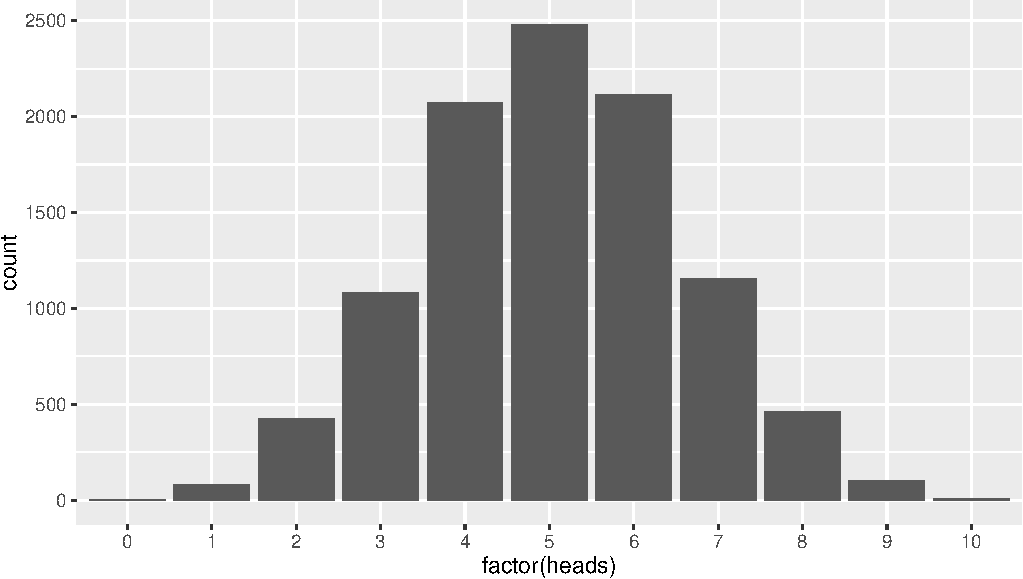
\includegraphics[width=\textwidth]{ismaykim_files/figure-latex/unnamed-chunk-78-1} 

}

\caption[Barplot of heads with p-value highlighted]{Barplot of heads with p-value highlighted}\label{fig:unnamed-chunk-78}
\end{figure}

This helps us better see just how few of the values of \texttt{heads}
are at our observed value or more extreme.

We'll see in Chapters \ref{hypo} and \ref{ci} that this idea of a
\(p\)-value can be extended to the more traditional methods using normal
and \(t\) distributions in the traditional way that introductory
statistics has been presented. These traditional methods were used
because statisticians haven't always been able to do 10,000 simulations
on the computer within seconds. We'll elaborate on this more in these
later chapters.

\begin{center}\rule{0.5\linewidth}{\linethickness}\end{center}

\begin{learncheck}
\textbf{\emph{Learning check}}
\end{learncheck}

\textbf{(LC7.6)} What is meant by ``pseudo-random number generation?''

\textbf{(LC7.7)} How can simulation be used to help us address the
question of whether or not an observed result is statistically
significant?

\textbf{(LC7.8)} In Chapter \ref{viz}, we noted that barplots should be
used when creating a plot of categorical variables. Why are we using
barplots to make a plot of a numerical variable \texttt{heads} in this
chapter?

\begin{center}\rule{0.5\linewidth}{\linethickness}\end{center}

\section{EXAMPLE: Comparing two
means}\label{example-comparing-two-means}

\subsection{Randomization/Permutation}\label{randomizationpermutation}

We will now focus on building hypotheses looking at the difference
between two population means in an example. We will denote population
means using the Greek symbol \(\mu\) (pronounced ``mu''). Thus, we will
be looking to see if one group ``out-performs'' another group. This is
quite possibly the most common type of statistical inference and serves
as a basis for many other types of analyses when comparing two groups.

Our null hypothesis will be of the form \(H_0: \mu_1 = \mu_2\), which
can also be written as \(H_0: \mu_1 - \mu_2 = 0\). Our alternative
hypothesis will be of the form \(H_0: \mu_1 \star \mu_2\) (or
\(H_a: \mu_1 - \mu_2 \, \star \, 0\)) where \(\star\) = \(<\), \(\ne\),
or \(>\) depending on the context of the problem. You needn't focus on
these new symbols too much at this point. It will just be a shortcut way
for us to describe our hypotheses.

As we saw earlier, simulation is a valuable tool when conducting
inferences based on one population variable. We will see that the
process of \textbf{randomization} (also known as \textbf{permutation})
will be valuable in conducting tests comparing quantitative values from
two groups.

\subsection{Comparing Action and Romance
Movies}\label{comparing-action-and-romance-movies}

The \texttt{movies} data set in the \texttt{ggplot2movies} package
contains information on a large number of movies that have been rated by
users of IMDB.com. We are interested in the question here of whether
\texttt{Action} movies are rated higher on IMDB than \texttt{Romance}
movies. We will first need to do a little bit of data manipulation using
the ideas from Chapter \ref{manip} to get the data in the form that we
would like:

\begin{Shaded}
\begin{Highlighting}[]
\KeywordTok{library}\NormalTok{(dplyr)}
\KeywordTok{library}\NormalTok{(ggplot2movies)}
\NormalTok{(movies_trimmed <-}\StringTok{ }\NormalTok{movies %>%}\StringTok{ }\KeywordTok{select}\NormalTok{(title, year, rating, Action, Romance))}
\end{Highlighting}
\end{Shaded}

\begin{verbatim}
## # A tibble: 58,788 × 5
##                       title  year rating Action Romance
##                       <chr> <int>  <dbl>  <int>   <int>
## 1                         $  1971    6.4      0       0
## 2         $1000 a Touchdown  1939    6.0      0       0
## 3    $21 a Day Once a Month  1941    8.2      0       0
## 4                   $40,000  1996    8.2      0       0
## 5  $50,000 Climax Show, The  1975    3.4      0       0
## 6                     $pent  2000    4.3      0       0
## 7                   $windle  2002    5.3      1       0
## 8                      '15'  2002    6.7      0       0
## 9                       '38  1987    6.6      0       0
## 10                  '49-'17  1917    6.0      0       0
## # ... with 58,778 more rows
\end{verbatim}

Note that \texttt{Action} and \texttt{Romance} are binary variables
here. To remove any overlap of movies (and potential confusion) that are
both \texttt{Action} and \texttt{Romance}, we will remove them from our
\emph{population}:

\begin{Shaded}
\begin{Highlighting}[]
\NormalTok{movies_trimmed <-}\StringTok{ }\NormalTok{movies_trimmed %>%}
\StringTok{  }\KeywordTok{filter}\NormalTok{(!(Action ==}\StringTok{ }\DecValTok{1} \NormalTok{&}\StringTok{ }\NormalTok{Romance ==}\StringTok{ }\DecValTok{1}\NormalTok{))}
\end{Highlighting}
\end{Shaded}

We will now create a new variable called \texttt{genre} that specifies
whether a movie in our \texttt{movies\_trimmed} data frame is an
\texttt{"Action"} movie, a \texttt{"Romance"} movie, or
\texttt{"Neither"}. We aren't really interested in the
\texttt{"Neither"} category here so we will exclude those rows as well.
Lastly, the \texttt{Action} and \texttt{Romance} columns are not needed
anymore since they are encoded in the \texttt{genre} column.

\begin{Shaded}
\begin{Highlighting}[]
\NormalTok{movies_trimmed <-}\StringTok{ }\NormalTok{movies_trimmed %>%}
\StringTok{  }\KeywordTok{mutate}\NormalTok{(}\DataTypeTok{genre =} \KeywordTok{ifelse}\NormalTok{(Action ==}\StringTok{ }\DecValTok{1}\NormalTok{, }\StringTok{"Action"}\NormalTok{,}
                        \KeywordTok{ifelse}\NormalTok{(Romance ==}\StringTok{ }\DecValTok{1}\NormalTok{, }\StringTok{"Romance"}\NormalTok{,}
                               \StringTok{"Neither"}\NormalTok{))) %>%}
\StringTok{  }\KeywordTok{filter}\NormalTok{(genre !=}\StringTok{ "Neither"}\NormalTok{) %>%}
\StringTok{  }\KeywordTok{select}\NormalTok{(-Action, -Romance)}
\end{Highlighting}
\end{Shaded}

We are left with 8878 movies in our \emph{population} data set that
focuses on only \texttt{"Action"} and \texttt{"Romance"} movies.

\begin{center}\rule{0.5\linewidth}{\linethickness}\end{center}

\begin{learncheck}
\textbf{\emph{Learning check}}
\end{learncheck}

\textbf{(LC7.9)} Why are the different genre variables stored as binary
variables (1s and 0s) instead of just listing the \texttt{genre} as a
column of values like ``Action'', ``Comedy'', etc.?

\textbf{(LC7.10)} What complications could come above with us excluding
action romance movies? Should we question the results of our hypothesis
test? Explain.

\begin{center}\rule{0.5\linewidth}{\linethickness}\end{center}

Let's now visualize the distributions of \texttt{rating} across both
levels of \texttt{genre}. Think about what type(s) of plot is/are
appropriate here before you proceed:

\begin{Shaded}
\begin{Highlighting}[]
\KeywordTok{library}\NormalTok{(ggplot2)}
\KeywordTok{ggplot}\NormalTok{(}\DataTypeTok{data =} \NormalTok{movies_trimmed, }\KeywordTok{aes}\NormalTok{(}\DataTypeTok{x =} \NormalTok{genre, }\DataTypeTok{y =} \NormalTok{rating)) +}
\StringTok{  }\KeywordTok{geom_boxplot}\NormalTok{()}
\end{Highlighting}
\end{Shaded}

\begin{figure}

{\centering 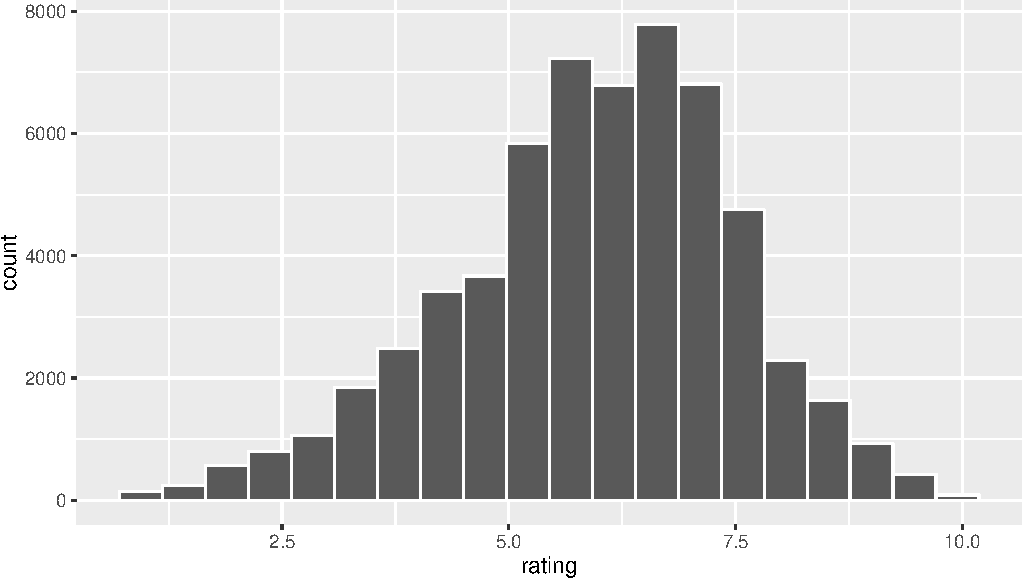
\includegraphics[width=\textwidth]{ismaykim_files/figure-latex/unnamed-chunk-82-1} 

}

\caption[Rating vs genre in the population]{Rating vs genre in the population}\label{fig:unnamed-chunk-82}
\end{figure}

We can see that the middle 50\% of ratings for \texttt{"Action"} movies
is more spread out than that of \texttt{"Romance"} movies in the
population. \texttt{"Romance"} has outliers at both the top and bottoms
of the scale though. We are initially interested in comparing the mean
\texttt{rating} across these two groups so a faceted histogram may also
be useful:

\begin{Shaded}
\begin{Highlighting}[]
\KeywordTok{ggplot}\NormalTok{(}\DataTypeTok{data =} \NormalTok{movies_trimmed, }\DataTypeTok{mapping =} \KeywordTok{aes}\NormalTok{(}\DataTypeTok{x =} \NormalTok{rating)) +}
\StringTok{  }\KeywordTok{geom_histogram}\NormalTok{(}\DataTypeTok{binwidth =} \DecValTok{1}\NormalTok{, }\DataTypeTok{color =} \StringTok{"white"}\NormalTok{, }\DataTypeTok{fill =} \StringTok{"dodgerblue"}\NormalTok{) +}
\StringTok{  }\KeywordTok{facet_grid}\NormalTok{(genre ~}\StringTok{ }\NormalTok{.)}
\end{Highlighting}
\end{Shaded}

\begin{figure}

{\centering 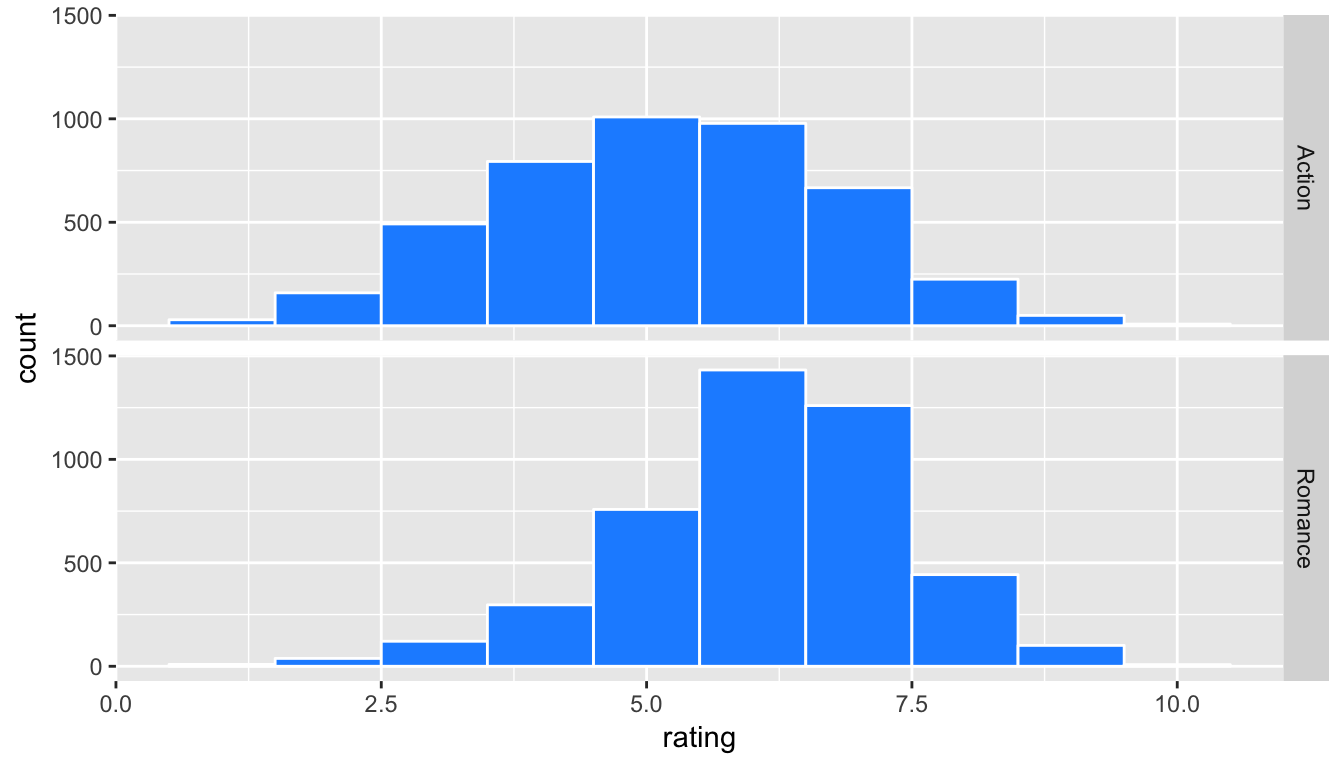
\includegraphics[width=\textwidth]{ismaykim_files/figure-latex/movie-hist-1} 

}

\caption[Faceted histogram of genre vs rating]{Faceted histogram of genre vs rating}\label{fig:movie-hist}
\end{figure}

\textbf{Important note:} Remember that we hardly ever have access to the
population values as we do here. This example and the
\texttt{nycflights13} data set were used to create a common flow from
chapter to chapter. In nearly all circumstances, we'll be needing to use
only a sample of the population to try to infer conclusions about the
unknown population parameter values. These examples do show a nice
relationship between statistics (where data is usually small and more
focused on experimental settings) and data science (where data is
frequently large and collected without experimental conditions).

\subsection{\texorpdfstring{Sampling \(\rightarrow\)
Randomization}{Sampling \textbackslash{}rightarrow Randomization}}\label{sampling-rightarrow-randomization}

We can use hypothesis testing to investigate ways to determine, for
example, whether a \textbf{treatment} has an effect over a
\textbf{control} and other ways to statistically analyze if one group
performs better than, worse than, or different than another. We will
also use confidence intervals to determine the size of the effect if it
exists. You'll see more on this in Chapter \ref{ci}.

We are interested here in seeing how we can use a random sample of
action movies and a random sample of romance movies from \texttt{movies}
to determine if a statistical difference exists in the mean ratings of
each group.

\begin{center}\rule{0.5\linewidth}{\linethickness}\end{center}

\begin{learncheck}
\textbf{\emph{Learning check}}
\end{learncheck}

\textbf{(LC7.11)} Define the relevant parameters here in terms of the
populations of movies.

\begin{center}\rule{0.5\linewidth}{\linethickness}\end{center}

\subsection{Data}\label{data-1}

Let's select a random sample of 34 action movies and a random sample of
34 romance movies. (The number 34 was chosen somewhat arbitrarily here.)

\begin{Shaded}
\begin{Highlighting}[]
\KeywordTok{library}\NormalTok{(dplyr)}
\KeywordTok{library}\NormalTok{(mosaic)}
\KeywordTok{set.seed}\NormalTok{(}\DecValTok{2016}\NormalTok{)}
\NormalTok{movies_genre_sample <-}\StringTok{ }\NormalTok{movies_trimmed %>%}\StringTok{ }
\StringTok{  }\KeywordTok{group_by}\NormalTok{(genre) %>%}
\StringTok{  }\KeywordTok{sample_n}\NormalTok{(}\DecValTok{34}\NormalTok{)}
\end{Highlighting}
\end{Shaded}

We can now observe the distributions of our two sample ratings for both
groups. Remember that these plots should be rough approximations of our
population distributions of movie ratings for \texttt{"Action"} and
\texttt{"Romance"} in our population of all movies in the
\texttt{movies} data frame.

\begin{Shaded}
\begin{Highlighting}[]
 \KeywordTok{ggplot}\NormalTok{(}\DataTypeTok{data =} \NormalTok{movies_genre_sample, }\KeywordTok{aes}\NormalTok{(}\DataTypeTok{x =} \NormalTok{genre, }\DataTypeTok{y =} \NormalTok{rating)) +}
\StringTok{  }\KeywordTok{geom_boxplot}\NormalTok{()}
\end{Highlighting}
\end{Shaded}

\begin{figure}

{\centering 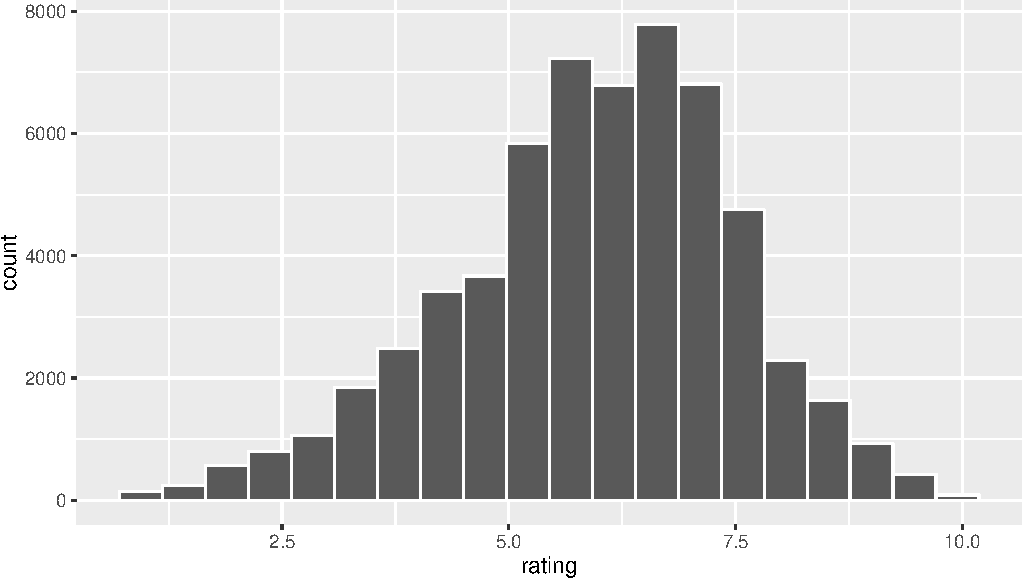
\includegraphics[width=\textwidth]{ismaykim_files/figure-latex/unnamed-chunk-84-1} 

}

\caption[Genre vs rating for our sample]{Genre vs rating for our sample}\label{fig:unnamed-chunk-84}
\end{figure}

\begin{Shaded}
\begin{Highlighting}[]
\KeywordTok{ggplot}\NormalTok{(}\DataTypeTok{data =} \NormalTok{movies_genre_sample, }\DataTypeTok{mapping =} \KeywordTok{aes}\NormalTok{(}\DataTypeTok{x =} \NormalTok{rating)) +}
\StringTok{  }\KeywordTok{geom_histogram}\NormalTok{(}\DataTypeTok{binwidth =} \DecValTok{1}\NormalTok{, }\DataTypeTok{color =} \StringTok{"white"}\NormalTok{, }\DataTypeTok{fill =} \StringTok{"dodgerblue"}\NormalTok{) +}
\StringTok{  }\KeywordTok{facet_grid}\NormalTok{(genre ~}\StringTok{ }\NormalTok{.)}
\end{Highlighting}
\end{Shaded}

\begin{figure}

{\centering 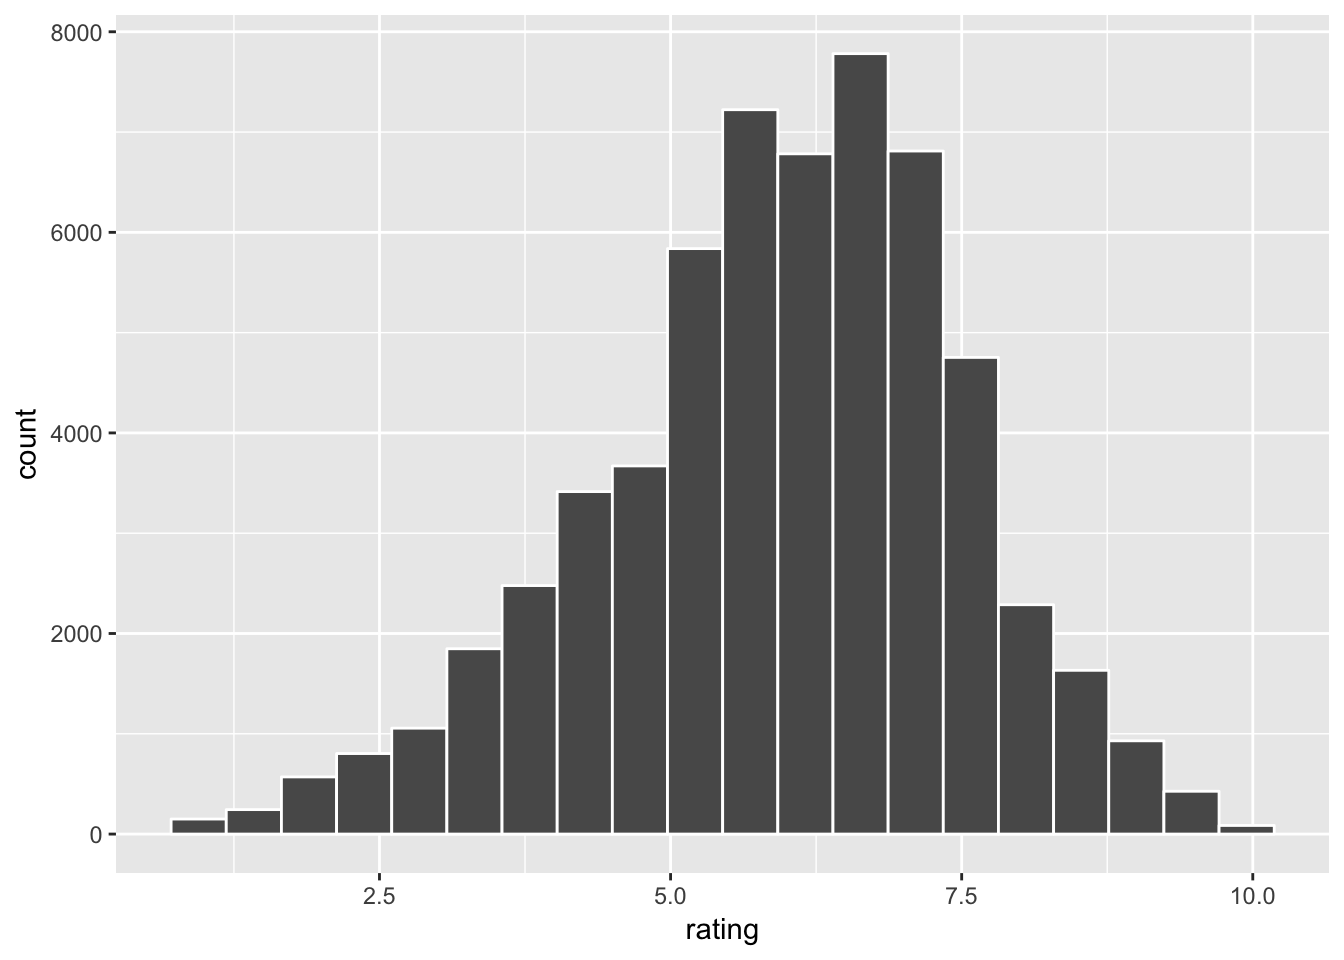
\includegraphics[width=\textwidth]{ismaykim_files/figure-latex/unnamed-chunk-85-1} 

}

\caption[Genre vs rating for our sample as faceted histogram]{Genre vs rating for our sample as faceted histogram}\label{fig:unnamed-chunk-85}
\end{figure}

\begin{center}\rule{0.5\linewidth}{\linethickness}\end{center}

\begin{learncheck}
\textbf{\emph{Learning check}}
\end{learncheck}

\textbf{(LC7.12)} What single value could we change to improve the
approximation using the sample distribution on the population
distribution?

\begin{center}\rule{0.5\linewidth}{\linethickness}\end{center}

Do we have reason to believe, based on the sample distributions of
\texttt{rating} over the two groups of \texttt{genre}, that there is a
significant difference between the mean \texttt{rating} for action
movies compared to romance movies? It's hard to say just based on the
plots. The boxplot does show that the median sample rating is higher for
romance movies, but the histogram isn't as clear. The two groups have
somewhat differently shaped distributions but they are both over similar
values of \texttt{rating}. It's often useful to calculate the mean and
standard deviation as well, conditioned on the two levels.

\begin{Shaded}
\begin{Highlighting}[]
\NormalTok{summary_ratings <-}\StringTok{ }\NormalTok{movies_genre_sample %>%}\StringTok{ }
\StringTok{  }\KeywordTok{group_by}\NormalTok{(genre) %>%}
\StringTok{  }\KeywordTok{summarize}\NormalTok{(}\DataTypeTok{mean =} \KeywordTok{mean}\NormalTok{(rating),}
            \DataTypeTok{std_dev =} \KeywordTok{sd}\NormalTok{(rating),}
            \DataTypeTok{n =} \KeywordTok{n}\NormalTok{())}
\NormalTok{summary_ratings}
\end{Highlighting}
\end{Shaded}

\begin{verbatim}
## # A tibble: 2 × 4
##     genre     mean  std_dev     n
##     <chr>    <dbl>    <dbl> <int>
## 1  Action 5.197059 1.464837    34
## 2 Romance 6.026471 1.202096    34
\end{verbatim}

\begin{center}\rule{0.5\linewidth}{\linethickness}\end{center}

\begin{learncheck}
\textbf{\emph{Learning check}}
\end{learncheck}

\textbf{(LC7.13)} Why did we not specify \texttt{na.rm\ =\ TRUE} here as
we did in Chapter \ref{manip}?

\begin{center}\rule{0.5\linewidth}{\linethickness}\end{center}

We see that the sample mean rating for romance movies, \(\bar{x}_{r}\),
is greater than the similar measure for action movies, \(\bar{x}_a\).
But is it statistically significantly greater (thus, leading us to
conclude that the means are statistically different)? The standard
deviation can provide some insight here but with these standard
deviations being so similar it's still hard to say for sure.

\begin{center}\rule{0.5\linewidth}{\linethickness}\end{center}

\begin{learncheck}
\textbf{\emph{Learning check}}
\end{learncheck}

\textbf{(LC7.14)} Why might the standard deviation provide some insight
about the means being statistically different or not?

\begin{center}\rule{0.5\linewidth}{\linethickness}\end{center}

\subsection{\texorpdfstring{Model of
\(H_0\)}{Model of H\_0}}\label{model-of-h_0-1}

The hypotheses we specified can also be written in another form to
better give us an idea of what we will be simulating to create our null
distribution.

\begin{itemize}
\tightlist
\item
  \(H_0: \mu_r - \mu_a = 0\)
\item
  \(H_a: \mu_r - \mu_a \ne 0\)
\end{itemize}

\subsection{\texorpdfstring{Test Statistic
\(\delta\)}{Test Statistic \textbackslash{}delta}}\label{test-statistic-delta-1}

We are, therefore, interested in seeing whether the difference in the
sample means, \(\bar{x}_r - \bar{x}_a\), is statistically different than
0. R has a built-in command that can calculate the difference in these
two sample means.

\subsection{\texorpdfstring{Observed effect
\(\delta^*\)}{Observed effect \textbackslash{}delta\^{}*}}\label{observed-effect-delta-1}

\begin{Shaded}
\begin{Highlighting}[]
\NormalTok{mean_ratings <-}\StringTok{ }\NormalTok{movies_genre_sample %>%}\StringTok{ }\KeywordTok{group_by}\NormalTok{(genre) %>%}
\StringTok{  }\KeywordTok{summarize}\NormalTok{(}\DataTypeTok{mean =} \KeywordTok{mean}\NormalTok{(rating))}
\NormalTok{obs_diff <-}\StringTok{ }\KeywordTok{diff}\NormalTok{(mean_ratings$mean)}
\end{Highlighting}
\end{Shaded}

We see here that the \texttt{diff} function calculates
\(\bar{x}_r - \bar{x}_a = 6.0264706 - 5.1970588 = 0.8294118\). We will
now proceed similarly to how we conducted the hypothesis test above for
the Lady Tasting Tea using simulation. Our goal is figure out a random
process with which to simulate the null hypothesis being true. Earlier
in this chapter, we used flipping of a fair coin as the random process
we were simulating with the null hypothesis being true
(\(H_0: \tau = 5\)).

\subsection{Simulated Data}\label{simulated-data-1}

\textbf{Tactile simulation}

Here, with us assuming the two population means are equal
(\(H_0: \mu_r - \mu_a = 0\)), we can look at this from a tactile point
of view by using index cards. There are \(n_r = 34\) data elements
corresponding to romance movies and \(n_a = 34\) for action movies. We
can write the 34 ratings from our sample for romance movies on one set
of 34 index cards and the 34 ratings for action movies on another set of
34 index cards. (Note that the sample sizes need not be the same.)

The next step is to put the two stacks of index cards together, creating
a new set of 68 cards. If we assume that the two population means are
equal, we are saying that there is no association between ratings and
genre (romance vs action). We can use the index cards to create two
\textbf{new} stacks for romance and action movies. First, we must
shuffle all the cards thoroughly. After doing so, in this case with
equal values of sample sizes, we split the deck in half.

We then calculate the new sample mean rating of the romance deck, and
also the new sample mean rating of the action deck. This creates one
simulation of the samples that were collected originally. We next want
to calculate a statistic from these two samples. Instead of actually
doing the calculation using index cards, we can use R as we have before
to simulate this process.

\begin{center}\rule{0.5\linewidth}{\linethickness}\end{center}

\begin{learncheck}
\textbf{\emph{Learning check}}
\end{learncheck}

\textbf{(LC7.15)} How would the tactile shuffling of index cards change
if we had different samples of say 20 action movies and 60 romance
movies? Describe each step that would change.

\textbf{(LC7.16)} Why are we taking the difference in the means of the
cards in the new shuffled decks?

\begin{center}\rule{0.5\linewidth}{\linethickness}\end{center}

\begin{Shaded}
\begin{Highlighting}[]
\KeywordTok{library}\NormalTok{(mosaic)}
\NormalTok{shuffled_ratings <-}\StringTok{ }\NormalTok{movies_trimmed %>%}
\StringTok{     }\KeywordTok{mutate}\NormalTok{(}\DataTypeTok{genre =} \KeywordTok{shuffle}\NormalTok{(genre)) %>%}\StringTok{ }
\StringTok{     }\KeywordTok{group_by}\NormalTok{(genre) %>%}
\StringTok{     }\KeywordTok{summarize}\NormalTok{(}\DataTypeTok{mean =} \KeywordTok{mean}\NormalTok{(rating))}
\KeywordTok{diff}\NormalTok{(shuffled_ratings$mean)}
\end{Highlighting}
\end{Shaded}

\begin{verbatim}
## [1] -0.0170207
\end{verbatim}

\subsection{\texorpdfstring{Distribution of \(\delta\) under
\(H_0\)}{Distribution of \textbackslash{}delta under H\_0}}\label{distribution-of-delta-under-h_0-1}

The only new command here is \texttt{shuffle} from the \texttt{mosaic}
package, which does what we would expect it to do. It simulates a
shuffling of the ratings between the two levels of \texttt{genre} just
as we could have done with index cards. We can now proceed in a similar
way to what we have done previously with the Lady Tasting Tea example by
repeating this process many times to create a \emph{null distribution}
of simulated differences in sample means.

\begin{Shaded}
\begin{Highlighting}[]
\KeywordTok{set.seed}\NormalTok{(}\DecValTok{2016}\NormalTok{)}
\NormalTok{many_shuffles <-}\StringTok{ }\KeywordTok{do}\NormalTok{(}\DecValTok{10000}\NormalTok{) *}\StringTok{ }
\StringTok{  }\NormalTok{(movies_trimmed %>%}
\StringTok{     }\KeywordTok{mutate}\NormalTok{(}\DataTypeTok{rating =} \KeywordTok{shuffle}\NormalTok{(rating)) %>%}\StringTok{ }
\StringTok{     }\KeywordTok{group_by}\NormalTok{(genre) %>%}
\StringTok{     }\KeywordTok{summarize}\NormalTok{(}\DataTypeTok{mean =} \KeywordTok{mean}\NormalTok{(rating))}
   \NormalTok{)}
\end{Highlighting}
\end{Shaded}

It is a good idea here to \texttt{View} the \texttt{many\_shuffles} data
frame via \texttt{View(many\_shuffles)}. We need to figure out a way to
subtract the first value of \texttt{mean} from the second value of
\texttt{mean} for each of the 10,000 simulations. This is a little
tricky but the \texttt{group\_by} function comes to our rescue here:

\begin{Shaded}
\begin{Highlighting}[]
\NormalTok{rand_distn <-}\StringTok{ }\NormalTok{many_shuffles %>%}
\StringTok{  }\KeywordTok{group_by}\NormalTok{(.index) %>%}
\StringTok{  }\KeywordTok{summarize}\NormalTok{(}\DataTypeTok{diffmean =} \KeywordTok{diff}\NormalTok{(mean))}
\end{Highlighting}
\end{Shaded}

We can now plot the distribution of these simulated differences in
means:

\begin{Shaded}
\begin{Highlighting}[]
\KeywordTok{ggplot}\NormalTok{(}\DataTypeTok{data =} \NormalTok{rand_distn, }\KeywordTok{aes}\NormalTok{(}\DataTypeTok{x =} \NormalTok{diffmean)) +}
\StringTok{  }\KeywordTok{geom_histogram}\NormalTok{(}\DataTypeTok{color =} \StringTok{"white"}\NormalTok{, }\DataTypeTok{bins =} \DecValTok{20}\NormalTok{)}
\end{Highlighting}
\end{Shaded}

\begin{figure}

{\centering \includegraphics[width=\textwidth]{ismaykim_files/figure-latex/unnamed-chunk-91-1} 

}

\caption[Simulated differences in means histogram]{Simulated differences in means histogram}\label{fig:unnamed-chunk-91}
\end{figure}

\subsection{The p-value}\label{the-p-value-1}

Remember that we are interested in seeing where our observed sample mean
difference of 0.8294118 falls on this null/randomization distribution.
We are interested in simply a difference here so ``more extreme''
corresponds to values in both tails on the distribution. Let's shade our
null distribution to show a visual representation of our \(p\)-value:

\begin{Shaded}
\begin{Highlighting}[]
\KeywordTok{ggplot}\NormalTok{(}\DataTypeTok{data =} \NormalTok{rand_distn, }\KeywordTok{aes}\NormalTok{(}\DataTypeTok{x =} \NormalTok{diffmean, }\DataTypeTok{fill =} \NormalTok{(}\KeywordTok{abs}\NormalTok{(diffmean) >=}\StringTok{ }\NormalTok{obs_diff))) +}
\StringTok{  }\KeywordTok{geom_histogram}\NormalTok{(}\DataTypeTok{color =} \StringTok{"white"}\NormalTok{, }\DataTypeTok{bins =} \DecValTok{20}\NormalTok{)}
\end{Highlighting}
\end{Shaded}

\begin{figure}

{\centering \includegraphics[width=\textwidth]{ismaykim_files/figure-latex/unnamed-chunk-92-1} 

}

\caption[Shaded histogram to show p-value]{Shaded histogram to show p-value}\label{fig:unnamed-chunk-92}
\end{figure}

You may initially think there is an error here, but remember that the
observed difference in means was 0.8294118. It falls far outside the
range of simulated differences. We can add a vertical line to represent
both it and its negative (since this is a two-tailed test) instead:

\begin{Shaded}
\begin{Highlighting}[]
\KeywordTok{ggplot}\NormalTok{(}\DataTypeTok{data =} \NormalTok{rand_distn, }\KeywordTok{aes}\NormalTok{(}\DataTypeTok{x =} \NormalTok{diffmean)) +}
\StringTok{  }\KeywordTok{geom_histogram}\NormalTok{(}\DataTypeTok{color =} \StringTok{"white"}\NormalTok{, }\DataTypeTok{bins =} \DecValTok{100}\NormalTok{) +}
\StringTok{  }\KeywordTok{geom_vline}\NormalTok{(}\DataTypeTok{xintercept =} \NormalTok{obs_diff, }\DataTypeTok{color =} \StringTok{"red"}\NormalTok{) +}
\StringTok{  }\KeywordTok{geom_vline}\NormalTok{(}\DataTypeTok{xintercept =} \NormalTok{-obs_diff, }\DataTypeTok{color =} \StringTok{"red"}\NormalTok{)}
\end{Highlighting}
\end{Shaded}

\begin{figure}

{\centering \includegraphics[width=\textwidth]{ismaykim_files/figure-latex/unnamed-chunk-93-1} 

}

\caption[Histogram with vertical lines corresponding to observed statistic]{Histogram with vertical lines corresponding to observed statistic}\label{fig:unnamed-chunk-93}
\end{figure}

Based on this plot, we have no values as extreme or more extreme than
our observed effect in both directions so we have evidence supporting
the conclusion that the mean rating for romance movies is different from
that of action movies. (It doesn't really matter what significance level
was chosen in this case. Think about why.) The next important idea is to
better understand just how much higher of a mean rating can we expect
the romance movies to have compared to that of action movies. This can
be addressed by creating a 95\% confidence interval as we will explore
in Chapter \ref{ci}.

\begin{center}\rule{0.5\linewidth}{\linethickness}\end{center}

\begin{learncheck}
\textbf{\emph{Learning check}}
\end{learncheck}

\textbf{(LC7.17)} Conduct the same analysis comparing action movies
versus romantic movies using the median rating instead of the mean
rating? Make sure to use the \texttt{\%\textgreater{}\%} as much as
possible. What was different and what was the same?

\textbf{(LC7.18)} What conclusions can you make from viewing the faceted
histogram looking at \texttt{rating} versus \texttt{genre} that you
couldn't see when looking at the boxplot?

\textbf{(LC7.19)} Describe in a paragraph how we used Allen Downey's
diagram to conclude if a statistical difference existed between mean
movie ratings for action and romance movies.

\textbf{(LC7.20)} Why are we relatively confident that the distributions
of the sample ratings will be good approximations of the population
distributions of ratings for the two genres?

\textbf{(LC7.21)} Using the definition of ``\(p\)-value'', write in
words what the \(p\)-value represents for the hypothesis test above
comparing the mean rating of romance to action movies.

\textbf{(LC7.22)} What is the value of the \(p\)-value for the
hypothesis test comparing the mean rating of romance to action movies?

\textbf{(LC7.23)} Do the results of the hypothesis test match up with
the original plots we made looking at the population of movies? Why or
why not?

\begin{center}\rule{0.5\linewidth}{\linethickness}\end{center}

\subsection{Summary}\label{summary-5}

To review, these are the steps one would take whenever you'd like to do
a hypothesis test comparing values from the distributions of two groups:

\begin{itemize}
\item
  Simulate many samples using a random process that matches the way the
  original data were collected and that \emph{assumes the null
  hypothesis is true}.
\item
  Collect the values of a sample statistic for each sample created using
  this random process to build a \emph{randomization distribution}.
\item
  Assess the significance of the \emph{original} sample by determining
  where its sample statistic lies in the randomization distribution.
\item
  If the proportion of values as extreme or more extreme than the
  observed statistic in the randomization distribution is smaller than
  the pre-determined significance level \(\alpha\), we reject \(H_0\).
  Otherwise, we fail to reject \(H_0\). (If no significance level is
  given, one can assume \(\alpha = 0.05\).)
\end{itemize}

\section{Building theory-based methods using
computation}\label{theory-hypo}

As a point of reference, we will now discuss the traditional
theory-based way to conduct the hypothesis test for determining if there
is a statistically significant difference in the sample mean rating of
Action movies versus Romance movies. This method and ones like it work
very well when the assumptions are met in order to run the test. They
are based on probability models and distributions such as the normal and
\(t\)-distributions.

These traditional methods have been used for many decades back to the
time when researchers didn't have access to computers that could run
10,000 simulations in under a minute. They had to base their methods on
probability theory instead. Many fields and researchers continue to use
these methods and that is the biggest reason for their inclusion here.
It's important to remember that a \(t\)-test or a \(z\)-test is really
just an approximation of what you have seen in this chapter already
using simulation and randomization. The focus here is on understanding
how the shape of the \(t\)-curve comes about without digging big into
the mathematical underpinnings.

\subsection{\texorpdfstring{EXAMPLE: \(t\)-test for two independent
samples}{EXAMPLE: t-test for two independent samples}}\label{example-t-test-for-two-independent-samples}

What is commonly done in statistics is the process of normalization.
What this entails is calculating the mean and standard deviation of a
variable. Then you subtract the mean from each value of your variable
and divide by the standard deviation. The most common normalization is
known as the \(z\)-score. The formula for a \(z\)-score is
\[Z = \frac{x - \mu}{\sigma}\], where \(x\) represent the value of a
variable, \(\mu\) represents the mean of the variable, and \(\sigma\)
represents the standard deviation of the variable. \(z\)-scores are
normally distributed with mean 0 and standard deviation 1. They have the
common, bell-shaped pattern.

\begin{center}\includegraphics[width=\textwidth]{ismaykim_files/figure-latex/unnamed-chunk-94-1} \end{center}

Recall, that we hardly ever know the mean and standard deviation of the
population of interest. This is almost always the case when considering
the means of two independent groups. To help account for us not knowing
the population parameter values, we can use the sample statistics
instead, but this comes with a bit of a price in terms of complexity.

Another form of normalization occurs when we need to use the sample
standard deviations as estimates for the unknown population standard
deviations. This normalization is often called the \(t\)-score. For the
two independent samples case like what we have for comparing action
movies to romance movies, the formula is
\[T =\dfrac{ (\bar{x}_1 - \bar{x}_2) - (\mu_1 - \mu_2)}{ \sqrt{\dfrac{s_1^2}{n_1} + \dfrac{s_2^2}{n_2}}  }\]

There is a lot to try to unpack here.

\begin{itemize}
\tightlist
\item
  \(\bar{x}_1\) is the sample mean response of the first group
\item
  \(\bar{x}_2\) is the sample mean response of the second group
\item
  \(\mu_1\) is the population mean response of the first group
\item
  \(\mu_2\) is the population mean response of the second group
\item
  \(s_1\) is the sample standard deviation of the response of the first
  group
\item
  \(s_2\) is the sample standard deviation of the response of the second
  group
\item
  \(n_1\) is the sample size of the first group
\item
  \(n_2\) is the sample size of the second group
\end{itemize}

Assuming that the null hypothesis is true (\(H_0: \mu_1 - \mu_2 = 0\)),
\(T\) is said to be distributed following a \(t\) distribution with
degrees of freedom equal to the smaller value of \(n_1 - 1\) and
\(n_2 - 1\). The ``degrees of freedom'' can be thought of measuring how
different the \(t\) distribution will be as compared to a normal
distribution. Small sample sizes lead to small degrees of freedom and,
thus, \(t\) distributions that have more values in the tails of their
distributions. Large sample sizes lead to large degrees of freedom and,
thus, \(t\) distributions that closely align with the standard normal,
bell-shaped curve.

So, assuming \(H_0\) is true, our formula simplifies a bit:

\[T =\dfrac{ \bar{x}_1 - \bar{x}_2}{ \sqrt{\dfrac{s_1^2}{n_1} + \dfrac{s_2^2}{n_2}}  }\]

We have already built an approximation for what we think the
distribution of \(\delta = \bar{x}_1 - \bar{x}_2\) looks like using
randomization above. Recall this distribution:

\begin{Shaded}
\begin{Highlighting}[]
\KeywordTok{ggplot}\NormalTok{(}\DataTypeTok{data =} \NormalTok{rand_distn, }\KeywordTok{aes}\NormalTok{(}\DataTypeTok{x =} \NormalTok{diffmean)) +}
\StringTok{  }\KeywordTok{geom_histogram}\NormalTok{(}\DataTypeTok{color =} \StringTok{"white"}\NormalTok{, }\DataTypeTok{bins =} \DecValTok{20}\NormalTok{)}
\end{Highlighting}
\end{Shaded}

\begin{figure}

{\centering \includegraphics[width=\textwidth]{ismaykim_files/figure-latex/unnamed-chunk-95-1} 

}

\caption[Simulated differences in means histogram]{Simulated differences in means histogram}\label{fig:unnamed-chunk-95}
\end{figure}

If we'd like to have a guess as to what the distribution of \(T\) might
look like instead, we need only to divide every value in
\texttt{rand\_distn} by
\(\sqrt{\dfrac{s_1^2}{n_1} + \dfrac{s_2^2}{n_2}}\). As we did before, we
will assign Romance to be group 1 and Action to be group 2. (This was
done since Romance comes second alphabetically and the reason why we
have a number mismatch below with 1 and 2.) Remember that we've already
calculated these values:

\begin{Shaded}
\begin{Highlighting}[]
\KeywordTok{kable}\NormalTok{(summary_ratings)}
\end{Highlighting}
\end{Shaded}

\begin{tabular}{l|r|r|r}
\hline
genre & mean & std\_dev & n\\
\hline
Action & 5.197059 & 1.464837 & 34\\
\hline
Romance & 6.026471 & 1.202096 & 34\\
\hline
\end{tabular}

We will create some shortcuts here so you can see the value being
calculated for the denominator of \(T\).

\begin{Shaded}
\begin{Highlighting}[]
\NormalTok{s1 <-}\StringTok{ }\NormalTok{summary_ratings$std_dev[}\DecValTok{2}\NormalTok{]}
\NormalTok{s2 <-}\StringTok{ }\NormalTok{summary_ratings$std_dev[}\DecValTok{1}\NormalTok{]}
\NormalTok{n1 <-}\StringTok{ }\NormalTok{summary_ratings$n[}\DecValTok{2}\NormalTok{]}
\NormalTok{n2 <-}\StringTok{ }\NormalTok{summary_ratings$n[}\DecValTok{1}\NormalTok{]}
\end{Highlighting}
\end{Shaded}

Here, we have \(s_1 = 1.2020964\), \(s_2 = 1.4648374\), \(n_1 = 34\),
and \(n_2 = 34\).

We can calculate the denominator via

\begin{Shaded}
\begin{Highlighting}[]
\NormalTok{denom_T <-}\StringTok{ }\KeywordTok{sqrt}\NormalTok{( (s1^}\DecValTok{2} \NormalTok{/}\StringTok{ }\NormalTok{n1) +}\StringTok{ }\NormalTok{(s2^}\DecValTok{2} \NormalTok{/}\StringTok{ }\NormalTok{n2) )}
\end{Highlighting}
\end{Shaded}

Now if we divide all of the values of \texttt{diffmean} in
\texttt{rand\_distn} by \texttt{denom\_T} we can have a simulated
distribution of \(T\) test statistics instead:

\begin{Shaded}
\begin{Highlighting}[]
\NormalTok{rand_distn <-}\StringTok{ }\NormalTok{rand_distn %>%}\StringTok{ }
\StringTok{  }\KeywordTok{mutate}\NormalTok{(}\DataTypeTok{t_stat =} \NormalTok{diffmean /}\StringTok{ }\NormalTok{denom_T)}
\KeywordTok{ggplot}\NormalTok{(}\DataTypeTok{data =} \NormalTok{rand_distn, }\KeywordTok{aes}\NormalTok{(}\DataTypeTok{x =} \NormalTok{t_stat)) +}
\StringTok{  }\KeywordTok{geom_histogram}\NormalTok{(}\DataTypeTok{color =} \StringTok{"white"}\NormalTok{, }\DataTypeTok{bins =} \DecValTok{20}\NormalTok{)}
\end{Highlighting}
\end{Shaded}

\begin{figure}

{\centering \includegraphics[width=\textwidth]{ismaykim_files/figure-latex/unnamed-chunk-99-1} 

}

\caption[Simulated T statistics histogram]{Simulated T statistics histogram}\label{fig:unnamed-chunk-99}
\end{figure}

We see that the shape of this distribution is the same as that of
\texttt{diffmean}. The scale has changed though with \texttt{t\_stat}
having less spread than \texttt{diffmean}.

A traditional \(t\)-test doesn't look at this simulated distribution,
but instead it looks at the \(t\)-curve with degrees of freedom equal to
33 (the minimum of \(n_1 = 34 - 1 = 33\) and \(n_2 = 34 - 1 = 33\)). We
now overlay what this \(t\)-curve looks like on top of the histogram
showing the simulated \(T\) statistics.

\begin{Shaded}
\begin{Highlighting}[]
\KeywordTok{ggplot}\NormalTok{(}\DataTypeTok{data =} \NormalTok{rand_distn, }\DataTypeTok{mapping =} \KeywordTok{aes}\NormalTok{(}\DataTypeTok{x =} \NormalTok{t_stat)) +}
\StringTok{  }\KeywordTok{geom_histogram}\NormalTok{(}\KeywordTok{aes}\NormalTok{(}\DataTypeTok{y =} \NormalTok{..density..), }\DataTypeTok{color =} \StringTok{"white"}\NormalTok{, }\DataTypeTok{binwidth =} \FloatTok{0.1}\NormalTok{) +}
\StringTok{  }\KeywordTok{stat_function}\NormalTok{(}\DataTypeTok{fun =} \NormalTok{dt,}
    \DataTypeTok{args =} \KeywordTok{list}\NormalTok{(}\DataTypeTok{df =} \KeywordTok{min}\NormalTok{(n1 -}\StringTok{ }\DecValTok{1}\NormalTok{, n2 -}\StringTok{ }\DecValTok{1}\NormalTok{)), }
    \DataTypeTok{color =} \StringTok{"royalblue"}\NormalTok{, }\DataTypeTok{size =} \DecValTok{2}\NormalTok{)}
\end{Highlighting}
\end{Shaded}

\begin{center}\includegraphics[width=\textwidth]{ismaykim_files/figure-latex/unnamed-chunk-100-1} \end{center}

We can see that the curve does a good job of approximating the
randomization distribution here. (More on when to expect for this to be
the case when we discuss conditions for the \(t\)-test in a bit.) To
calculate the \(p\)-value in this case, we need to figure out how much
of the total area under the \(t\)-curve is at our observed
\(T\)-statistic or more, plus also adding the area under the curve at
the negative value of the observed \(T\)-statistic or below. (Remember
this is a two-tailed test so we are looking for a difference--values in
the tails of either direction.) Just as we converted all of the
simulated values to \(T\)-statistics, we must also do so for our
observed effect \(\delta^*\):

\begin{Shaded}
\begin{Highlighting}[]
\NormalTok{(t_obs <-}\StringTok{ }\NormalTok{obs_diff /}\StringTok{ }\NormalTok{denom_T)}
\end{Highlighting}
\end{Shaded}

\begin{verbatim}
## [1] 2.552202
\end{verbatim}

So graphically we are interested in finding the percentage of values
that are at or above 2.5522017 or at or below -2.5522017.

\begin{Shaded}
\begin{Highlighting}[]
\KeywordTok{ggplot}\NormalTok{(}\DataTypeTok{data =} \NormalTok{rand_distn, }\DataTypeTok{mapping =} \KeywordTok{aes}\NormalTok{(}\DataTypeTok{x =} \NormalTok{t_stat)) +}
\StringTok{  }\KeywordTok{stat_function}\NormalTok{(}\DataTypeTok{fun =} \NormalTok{dt,}
    \DataTypeTok{args =} \KeywordTok{list}\NormalTok{(}\DataTypeTok{df =} \KeywordTok{min}\NormalTok{(n1 -}\StringTok{ }\DecValTok{1}\NormalTok{, n2 -}\StringTok{ }\DecValTok{1}\NormalTok{)), }
    \DataTypeTok{color =} \StringTok{"royalblue"}\NormalTok{, }\DataTypeTok{size =} \DecValTok{2}\NormalTok{) +}
\StringTok{  }\KeywordTok{geom_vline}\NormalTok{(}\DataTypeTok{xintercept =} \NormalTok{t_obs, }\DataTypeTok{color =} \StringTok{"red"}\NormalTok{) +}
\StringTok{  }\KeywordTok{geom_vline}\NormalTok{(}\DataTypeTok{xintercept =} \NormalTok{-t_obs, }\DataTypeTok{color =} \StringTok{"red"}\NormalTok{)}
\end{Highlighting}
\end{Shaded}

\begin{center}\includegraphics[width=\textwidth]{ismaykim_files/figure-latex/unnamed-chunk-102-1} \end{center}

At this point, you should make a guess as to what a reasonable value may
be for the \(p\)-value. Let's say the \(p\)-value is 0.01 or so. To
actually perform this calculation by hand, you'd need to do some
calculus. Let's have R do it for us instead using the \texttt{pt}
function.

\begin{Shaded}
\begin{Highlighting}[]
\KeywordTok{pt}\NormalTok{(t_obs, }\DataTypeTok{df =} \KeywordTok{min}\NormalTok{(n1 -}\StringTok{ }\DecValTok{1}\NormalTok{, n2 -}\StringTok{ }\DecValTok{1}\NormalTok{), }\DataTypeTok{lower.tail =} \OtherTok{FALSE}\NormalTok{) +}
\StringTok{  }\KeywordTok{pt}\NormalTok{(-t_obs, }\DataTypeTok{df =} \KeywordTok{min}\NormalTok{(n1 -}\StringTok{ }\DecValTok{1}\NormalTok{, n2 -}\StringTok{ }\DecValTok{1}\NormalTok{), }\DataTypeTok{lower.tail =} \OtherTok{TRUE}\NormalTok{)}
\end{Highlighting}
\end{Shaded}

\begin{verbatim}
## [1] 0.01551859
\end{verbatim}

\subsection{Conditions for t-test}\label{conditions-for-t-test}

In order for the results of the \(t\)-test to be valid, three conditions
must be met:

\begin{enumerate}
\def\labelenumi{\arabic{enumi}.}
\tightlist
\item
  Independent observations in both samples
\item
  Nearly normal populations OR large sample sizes (\(n \ge 30\))
\item
  Independently selected samples
\end{enumerate}

Condition 1: This is met since we sampled at random using R from our
population.

Condition 2: Recall from Figure \ref{fig:movie-hist}, that we know how
the populations are distributed. Both of them are close to normally
distributed. If we are a little concerned about this assumption, we also
do have samples of size larger than 30 (\(n_1 = n_2 = 34\)).

Condition 3: This is met since there is no natural pairing of a movie in
the Action group to a movie in the Romance group.

Since all three conditions are met, we can be reasonably certain that
the theory-based test will match the results of the randomization-based
test using shuffling. Remember that theory-based tests can produce some
incorrect results in these assumptions are not carefully checked. The
only assumption for randomization and computational-based methods is
that the sample is selected at random. They are our preference and we
strongly believe they should be yours as well, but it's important to
also see how the theory-based tests can be done and used as an
approximation for the computational techniques until at least more
researchers are using these techniques that utilize the power of
computers.

\section{Conclusion}\label{conclusion-3}

\subsection{Script of R code}\label{script-of-r-code-3}

An R script file of all R code used in this chapter is available
\href{http://ismayc.github.io/moderndiver-book/07-hypo.R}{here}.

\subsection{What's to come?}\label{whats-to-come-4}

This chapter examined the basics of hypothesis testing with terminology
and also an example of how to apply the ``There is Only One Test''
diagram to the Lady Tasting Tea example presented in Chapter \ref{sim}
and to an example on comparing the IMDB ratings of action movies and
romance movies. We'll see in Chapter \ref{ci} how we can provide a range
of possible values for an unknown population parameter instead of just
running a Yes/No decision from a hypothesis test.

We will see in Chapter \ref{regress} many of the same ideas we have seen
with hypothesis testing and confidence intervals in the last two
chapters. Regression is frequently associated both correctly and
incorrectly with statistics and data analysis, so you'll need to make
sure you understand when it is appropriate and when it is not.

\chapter{Confidence Intervals}\label{ci}

\begin{center}\rule{0.5\linewidth}{\linethickness}\end{center}

\textbf{Definition: Confidence Interval}

A \emph{confidence interval} gives a range of plausible values for a
parameter. It depends on a specified \emph{confidence level} with higher
confidence levels corresponding to wider confidence intervals and lower
confidence levels corresponding to narrower confidence intervals. Common
confidence levels include 90\%, 95\%, and 99\%.

\begin{center}\rule{0.5\linewidth}{\linethickness}\end{center}

Usually we don't just begin chapters with a definition, but
\emph{confidence intervals} are simple to define and play an important
role in the sciences and any field that uses data. You can think of a
confidence interval as playing the role of a net when fishing. Instead
of just trying to catch a fish with a single spear (estimating an
unknown parameter by using a single point estimate/statistic), we can
use a net to try to provide a range of possible locations for the fish
(use a range of possible values based around our statistic to make a
plausible guess as to the location of the parameter).

\section*{Needed packages}\label{needed-packages-4}
\addcontentsline{toc}{section}{Needed packages}

\begin{Shaded}
\begin{Highlighting}[]
\KeywordTok{library}\NormalTok{(dplyr)}
\KeywordTok{library}\NormalTok{(ggplot2)}
\KeywordTok{library}\NormalTok{(mosaic)}
\KeywordTok{library}\NormalTok{(knitr)}
\end{Highlighting}
\end{Shaded}

\section{Bootstrapping}\label{bootstrapping}

Just as we did in Chapter \ref{hypo} with the Lady Tasting Tea when
making hypotheses about a population total with which we would like to
test which one is more plausible, we can also use simulation to infer
conclusions about a population quantitative statistic such as the mean.
In this case, we will focus on constructing confidence intervals to
produce plausible values for a population mean. (We can do a similar
analysis for a population median or other summary measure as well.)

Traditionally, the way to construct confidence intervals for a mean is
to assume a normal distribution for the population or to invoke the
Central Limit Theorem and get, what often appears to be magic, results.
(This is similar to what was done in Section \ref{theory-hypo}.) These
methods are often not intuitive, especially for those that lack a strong
mathematical background. They also come with their fair share of
assumptions and often turn Statistics, a field that is full of tons of
useful applications to many different fields and disciplines, into a
robotic procedural-based topic. It doesn't have to be that way!

In this section, we will introduce the concept of
\textbf{bootstrapping}. It will be a useful tool that will allow us to
estimate the variability of our statistic from sample to sample. One
neat feature of bootstrapping is that it enables us to approximate the
sampling distribution and estimate the distribution's standard deviation
using ONLY the information in the one selected (original) sample.

It sounds just as plagued with the magical type qualities of traditional
theory-based inference on initial glance but we will see that it
provides an intuitive and useful way to make inferences, especially when
the samples are of medium to large size.

To introduce the concept of bootstrapping, we again will use the
\texttt{movies} data set in the \texttt{ggplot2movies} data frame.
Remember that we load this data frame into R in much the same way as we
loaded \texttt{flights} and \texttt{weather} from the
\texttt{nycflights13} package.

\begin{Shaded}
\begin{Highlighting}[]
\KeywordTok{library}\NormalTok{(ggplot2movies)}
\KeywordTok{data}\NormalTok{(movies, }\DataTypeTok{package =} \StringTok{"ggplot2movies"}\NormalTok{)}
\end{Highlighting}
\end{Shaded}

Recall that you can also glance at this data frame using the
\texttt{View} function and look at the help documentation for
\texttt{movies} using the \texttt{?} function.

We will explore many other features of this data set in the chapters to
come, but here we will be focusing on the \texttt{rating} variable
corresponding to the average IMDB user rating.

You may notice that this data set is quite large: 58,788 movies have
data collected about them here. This will correspond to our population
of ALL movies. Remember from Chapter \ref{sim} that our population is
rarely known. We use this data set as our population here to show you
the power of bootstrapping in estimating population parameters. We'll
see how \textbf{confidence intervals} built using the bootstrap
distribution do at including our population parameter of interest. Here
we can actually calculate these values since our population is known,
but remember that in general this isn't the case.

Let's take a look at what the distribution of our population
\texttt{ratings} looks like. We'll see that we will use the distribution
of our sample(s) as an estimate of this population histogram.

\begin{Shaded}
\begin{Highlighting}[]
\NormalTok{movies %>%}\StringTok{ }\KeywordTok{ggplot}\NormalTok{(}\KeywordTok{aes}\NormalTok{(}\DataTypeTok{x =} \NormalTok{rating)) +}
\StringTok{  }\KeywordTok{geom_histogram}\NormalTok{(}\DataTypeTok{color =} \StringTok{"white"}\NormalTok{, }\DataTypeTok{bins =} \DecValTok{20}\NormalTok{)}
\end{Highlighting}
\end{Shaded}

\begin{figure}

{\centering \includegraphics[width=\textwidth]{ismaykim_files/figure-latex/unnamed-chunk-107-1} 

}

\caption[Population ratings histogram]{Population ratings histogram}\label{fig:unnamed-chunk-107}
\end{figure}

\begin{center}\rule{0.5\linewidth}{\linethickness}\end{center}

\begin{learncheck}
\textbf{\emph{Learning check}}
\end{learncheck}

\textbf{(LC8.1)} Why was a histogram chosen as the plot to make for the
\texttt{rating} variable above?

\textbf{(LC8.2)} Why does the shape of the \texttt{rating} histogram
tell us about how IMDB users rate movies? What stands out about the
plot?

\begin{center}\rule{0.5\linewidth}{\linethickness}\end{center}

It's important to think about what our goal is here. We would like to
produce a confidence interval for the population mean \texttt{rating}.
We will have to pretend for a moment that we don't have all 58,788
movies. Let's say that we only have a random sample of 50 movies from
this data set instead. In order to get a random sample, we can use the
\texttt{resample} function in the \texttt{mosaic} package with
\texttt{replace\ =\ FALSE}. We could also use the \texttt{sample\_n}
function from \texttt{dplyr}.

\begin{Shaded}
\begin{Highlighting}[]
\KeywordTok{set.seed}\NormalTok{(}\DecValTok{2017}\NormalTok{)}
\KeywordTok{library}\NormalTok{(mosaic)}
\NormalTok{movies_sample <-}\StringTok{ }\NormalTok{movies %>%}\StringTok{ }\KeywordTok{resample}\NormalTok{(}\DataTypeTok{size =} \DecValTok{50}\NormalTok{, }\DataTypeTok{replace =} \OtherTok{FALSE}\NormalTok{)}
\end{Highlighting}
\end{Shaded}

The \texttt{resample} function has filtered the data frame
\texttt{movies} ``at random'' to choose only 50 rows from the larger
\texttt{movies} data frame. We store information on these 50 movies in
the \texttt{movies\_sample} data frame.

Let's now explore what the \texttt{rating} variable looks like for these
50 movies:

\begin{Shaded}
\begin{Highlighting}[]
\NormalTok{movies_sample %>%}\StringTok{ }\KeywordTok{ggplot}\NormalTok{(}\KeywordTok{aes}\NormalTok{(}\DataTypeTok{x =} \NormalTok{rating)) +}
\StringTok{  }\KeywordTok{geom_histogram}\NormalTok{(}\DataTypeTok{color =} \StringTok{"white"}\NormalTok{, }\DataTypeTok{bins =} \DecValTok{20}\NormalTok{)}
\end{Highlighting}
\end{Shaded}

\begin{figure}

{\centering \includegraphics[width=\textwidth]{ismaykim_files/figure-latex/unnamed-chunk-109-1} 

}

\caption[Sample ratings histogram]{Sample ratings histogram}\label{fig:unnamed-chunk-109}
\end{figure}

Remember that we can think of this histogram as an estimate of our
population distribution histogram that we saw above. We are interested
in the population mean rating and trying to find a range of plausible
values for that value. A good start in guessing the population mean is
to use the mean of our sample \texttt{rating} from the
\texttt{movies\_sample} data:

\begin{Shaded}
\begin{Highlighting}[]
\NormalTok{(movies_sample_mean <-}\StringTok{ }\NormalTok{movies_sample %>%}\StringTok{ }\KeywordTok{summarize}\NormalTok{(}\DataTypeTok{mean =} \KeywordTok{mean}\NormalTok{(rating)))}
\end{Highlighting}
\end{Shaded}

\begin{verbatim}
## # A tibble: 1 × 1
##    mean
##   <dbl>
## 1 5.894
\end{verbatim}

Note the use of the \texttt{(\ )} at the beginning and the end of this
creation of the \texttt{movies\_sample\_mean} object. If you'd like to
print out your newly created object, you can enclose it in the
parentheses as we have here.

This value of 5.894 is just one guess at the population mean. The idea
behind \emph{bootstrapping} is to sample \textbf{with replacement} from
the original sample to create new \textbf{resamples} of the same size as
our original sample.

Returning to our example, let's investigate what one such resample of
the \texttt{movies\_sample} data set accomplishes. We can create one
resample/bootstrap sample by using the \texttt{resample} function in the
\texttt{mosaic} package.

\begin{Shaded}
\begin{Highlighting}[]
\KeywordTok{library}\NormalTok{(mosaic)}
\NormalTok{boot1 <-}\StringTok{ }\KeywordTok{resample}\NormalTok{(movies_sample) %>%}
\StringTok{  }\KeywordTok{arrange}\NormalTok{(orig.id)}
\end{Highlighting}
\end{Shaded}

The important thing to note here is the original row numbers from the
\texttt{movies\_sample} data frame in the far right column called
\texttt{orig.ids}. Since we are sampling with replacement, there is a
strong likelihood that some of the 50 observational units are going to
be selected again.

You may be asking yourself what does this mean and how does this lead us
to creating a distribution for the sample mean. Recall that the original
sample mean of our data was calculated using the \texttt{summarize}
function above.

\begin{center}\rule{0.5\linewidth}{\linethickness}\end{center}

\begin{learncheck}
\textbf{\emph{Learning check}}
\end{learncheck}

\textbf{(LC8.3)} What happens if we change the seed to our pseudo-random
generation? Try it above when we used \texttt{resample} to describe the
resulting \texttt{movies\_sample}.

\textbf{(LC8.4)} Why is sampling at random important from the
\texttt{movies} data frame? Why don't we just pick \texttt{Action}
movies and do bootstrapping with this \texttt{Action} movies subset?

\textbf{(LC8.5)} What was the purpose of assuming we didn't have access
to the full \texttt{movies} data set here?

\begin{center}\rule{0.5\linewidth}{\linethickness}\end{center}

Before we had a calculated mean in our original sample of 5.894. Let's
calculate the mean of \texttt{ratings} in our bootstrapped sample:

\begin{Shaded}
\begin{Highlighting}[]
\NormalTok{(movies_boot1_mean <-}\StringTok{ }\NormalTok{boot1 %>%}\StringTok{ }\KeywordTok{summarize}\NormalTok{(}\DataTypeTok{mean =} \KeywordTok{mean}\NormalTok{(rating)))}
\end{Highlighting}
\end{Shaded}

\begin{verbatim}
## # A tibble: 1 × 1
##    mean
##   <dbl>
## 1 5.686
\end{verbatim}

More than likely the calculated bootstrap sample mean is different than
the original sample mean. This is what was meant earlier by the sample
means having some variability. What we are trying to do is replicate
many different samples being taken from a larger population. Our best
guess at what the population looks like is multiple copies of the sample
we collected. We then can sample from that larger ``created'' population
by generating bootstrap samples.

Similar to what we did in the previous section, we can repeat this
process using the \texttt{do} function followed by an asterisk. Let's
look at 10 different bootstrap means for \texttt{ratings} from
\texttt{movies\_sample}. Note the use of the \texttt{resample} function
here.

\begin{Shaded}
\begin{Highlighting}[]
\KeywordTok{do}\NormalTok{(}\DecValTok{10}\NormalTok{) *}\StringTok{ }
\StringTok{  }\NormalTok{(}\KeywordTok{resample}\NormalTok{(movies_sample) %>%}\StringTok{ }
\StringTok{     }\KeywordTok{summarize}\NormalTok{(}\DataTypeTok{mean =} \KeywordTok{mean}\NormalTok{(rating)))}
\end{Highlighting}
\end{Shaded}

\begin{verbatim}
##     mean
## 1  5.942
## 2  5.572
## 3  5.828
## 4  6.292
## 5  6.032
## 6  5.920
## 7  5.996
## 8  5.852
## 9  6.098
## 10 5.608
\end{verbatim}

You should see some variability begin to tease its way out here. Many of
the simulated means will be close to our original sample mean but many
will stray pretty far away. This occurs because outliers may have been
selected a couple of times in the resampling or small values were
selected more than larger. There are myriad reasons why this might be
the case.

So what's the next step now? Just as we repeated the repetitions
thousands of times with the ``Lady Tasting Tea'' example, we can do a
similar thing here.

\begin{Shaded}
\begin{Highlighting}[]
\NormalTok{trials <-}\StringTok{ }\KeywordTok{do}\NormalTok{(}\DecValTok{10000}\NormalTok{) *}\StringTok{ }\KeywordTok{summarize}\NormalTok{(}\KeywordTok{resample}\NormalTok{(movies_sample), }
                                \DataTypeTok{mean =} \KeywordTok{mean}\NormalTok{(rating))}
\KeywordTok{ggplot}\NormalTok{(}\DataTypeTok{data =} \NormalTok{trials, }\DataTypeTok{mapping =} \KeywordTok{aes}\NormalTok{(}\DataTypeTok{x =} \NormalTok{mean)) +}
\StringTok{  }\KeywordTok{geom_histogram}\NormalTok{(}\DataTypeTok{bins =} \DecValTok{30}\NormalTok{, }\DataTypeTok{color =} \StringTok{"white"}\NormalTok{)}
\end{Highlighting}
\end{Shaded}

\begin{figure}

{\centering \includegraphics[width=\textwidth]{ismaykim_files/figure-latex/unnamed-chunk-114-1} 

}

\caption[Bootstrapped means histogram]{Bootstrapped means histogram}\label{fig:unnamed-chunk-114}
\end{figure}

The shape of this resulting distribution may look familiar to you. It
resembles the well-known normal (bell-shaped) curve. At this point, we
can easily calculate a confidence interval. In fact, we have a couple
different options. We will first use the percentiles of the distribution
we just created to isolate the middle 95\% of values. This will
correspond to our 95\% confidence interval for the population mean
\texttt{rating}, denoted by \(\mu\).

\begin{Shaded}
\begin{Highlighting}[]
\NormalTok{(ciq_mean_rating <-}\StringTok{ }\KeywordTok{confint}\NormalTok{(trials, }\DataTypeTok{level =} \FloatTok{0.95}\NormalTok{, }\DataTypeTok{method =} \StringTok{"quantile"}\NormalTok{))}
\end{Highlighting}
\end{Shaded}

\begin{verbatim}
##   name lower upper level     method estimate
## 1 mean 5.456 6.296  0.95 percentile    5.894
\end{verbatim}

It's always important at this point to interpret the results of this
confidence interval calculation. In this context, we can say something
like the following:

\begin{quote}
Based on the sample data and bootstrapping techniques, we can be 95\%
confident that the true mean rating of ALL IMDB ratings is between 5.456
and 6.296.
\end{quote}

This statement may seem a little confusing to you. Another way to think
about this is that this confidence interval was constructed using the
sample data by a procedure that is \textbf{95\% reliable.} We will get
invalid results 5\% of the time. Just as we had a trade-off with
\(\alpha\) and \(\beta\) with hypothesis tests, we have a similar
trade-off here with setting the confidence level.

To further reiterate this point, the graphic below from \citet{isrs2014}
shows us that if we repeated a confidence interval process 25 times with
25 different samples, we would expect about 95\% of them to actually
contain the population parameter of interest. This parameter is marked
with a dotted vertical line. We can see that only one confidence
interval does not overlap with this value. (The one marked in red.)
Therefore 24 in 25 (96\%), which is quite close to our 95\% reliability,
do include the population parameter.

\begin{figure}

{\centering \includegraphics[width=\textwidth]{images/cis} 

}

\caption[Confidence interval coverage plot from OpenIntro]{Confidence interval coverage plot from OpenIntro}\label{fig:ci-coverage}
\end{figure}

Remember that we are pretending like we don't know what the mean IMDB
rating for ALL movies is. Our population here is all of the movies
listed in the \texttt{movies} data frame from \texttt{ggplot2movies}. So
does our bootstrapped confidence interval here contain the actual mean
value?

\begin{Shaded}
\begin{Highlighting}[]
\NormalTok{movies %>%}\StringTok{ }\KeywordTok{summarize}\NormalTok{(}\DataTypeTok{mean_rating =} \KeywordTok{mean}\NormalTok{(rating)) %>%}\StringTok{ }
\StringTok{  }\KeywordTok{kable}\NormalTok{()}
\end{Highlighting}
\end{Shaded}

\begin{tabular}{r}
\hline
mean\_rating\\
\hline
5.93285\\
\hline
\end{tabular}

We see here that the population mean does fall in our range of plausible
values generated from the bootstrapped samples.

We can also get an idea of how the theory-based inference techniques
would have approximated this confidence interval by using the formula
\[\bar{x} \pm (2 * SE),\] where \(\bar{x}\) is our original sample mean
and \(SE\) stands for \textbf{standard error} and corresponds to the
standard deviation of the bootstrap distribution. The value of 2 here
corresponds to it being a 95\% confidence interval. This formula assumes
that the bootstrap distribution is symmetric and bell-shaped. This is
often the case with bootstrap distributions, especially those in which
the original distribution of the sample is not highly skewed.

\begin{center}\rule{0.5\linewidth}{\linethickness}\end{center}

\textbf{Definition: standard error}

The \emph{standard error} is the standard deviation of the sampling
distribution. The sampling distribution may be approximated by the
bootstrap distribution or the null distribution depending on the
context. Traditional theory-based methodologies for inference also have
formulas for standard errors assuming some conditions are met.

\begin{center}\rule{0.5\linewidth}{\linethickness}\end{center}

To compute this type of confidence interval, we only need to make a
slight modification to the \texttt{confint} function seen above. (The
expression after the \(\pm\) sign is known as the \textbf{margin of
error}.)

\begin{Shaded}
\begin{Highlighting}[]
\NormalTok{(cise_mean_rating <-}\StringTok{ }\KeywordTok{confint}\NormalTok{(trials, }\DataTypeTok{level =} \FloatTok{0.95}\NormalTok{, }\DataTypeTok{method =} \StringTok{"stderr"}\NormalTok{))}
\end{Highlighting}
\end{Shaded}

\begin{verbatim}
##   name    lower    upper level method estimate margin.of.error
## 1 mean 5.468465 6.314277  0.95 stderr    5.894       0.4229063
\end{verbatim}

\begin{quote}
Based on the sample data and bootstrapping techniques, we can be 95\%
confident that the true mean rating of ALL IMDB ratings is between
5.4684649 and 6.3142775.
\end{quote}

\begin{center}\rule{0.5\linewidth}{\linethickness}\end{center}

\begin{learncheck}
\textbf{\emph{Learning check}}
\end{learncheck}

\textbf{(LC8.6)} Reproduce the bootstrapping above using a sample of
size 50 instead of 25. What changes do you see?

\textbf{(LC8.7)} Reproduce the bootstrapping above using a sample of
size 5 instead of 25. What changes do you see?

\textbf{(LC8.8)} How does the sample size affect the analysis?

\textbf{(LC8.9)} Why must bootstrap samples be the same size as the
original sample?

\begin{center}\rule{0.5\linewidth}{\linethickness}\end{center}

\subsection{Review of Bootstrapping}\label{review-of-bootstrapping}

We can summarize the process to generate a bootstrap distribution here
in a series of steps that clearly identify the terminology we will use
\citep{lock2012}.

\begin{itemize}
\tightlist
\item
  Generate \texttt{bootstrap\ samples} by sampling with replacement from
  the original sample, using the same sample size.
\item
  Compute the statistic of interest, called a
  \texttt{bootstrap\ statistic}, for each of the bootstrap samples.
\item
  Collect the statistics for many bootstrap samples to create a
  \texttt{bootstrap\ distribution}.
\end{itemize}

Visually, we can represent this process in the following diagram.

\begin{figure}

{\centering \includegraphics[width=\textwidth]{images/bootstrap} 

}

\caption[Bootstrapping diagram from Lock5 textbook]{Bootstrapping diagram from Lock5 textbook}\label{fig:bootstrapimg}
\end{figure}

\section{Relation to hypothesis
testing}\label{relation-to-hypothesis-testing}

Recall that we found a statistically significant difference in the
sample mean of romance movie ratings compared to the sample mean of
action movie ratings. We concluded Chapter \ref{hypo} by attempted to
understand just how much greater we could expect the \emph{population}
mean romance movie rating to be as compared to the \emph{population}
mean action movie rating. In order to do so, we will calculate a
confidence interval for the difference \(\mu_r - \mu_a\). We'll then go
back to our population parameter values and see if our confidence
interval contains our parameter value.

We could use bootstrapping in a way similar to that done above, except
now on a difference in sample means, to create a distribution and then
use the \texttt{confint} function with the option of \texttt{quantile}
to determine a confidence interval for the plausible values of the
difference in population means. This is an excellent programming
activity and the reader is urged to try to do so.

Recall what the randomization/null distribution looked like for our
simulated shuffled sample means:

\begin{Shaded}
\begin{Highlighting}[]
\KeywordTok{library}\NormalTok{(ggplot2)}
\KeywordTok{library}\NormalTok{(dplyr)}
\KeywordTok{ggplot}\NormalTok{(}\DataTypeTok{data =} \NormalTok{rand_distn, }\DataTypeTok{mapping =} \KeywordTok{aes}\NormalTok{(}\DataTypeTok{x =} \NormalTok{diffmean)) +}
\StringTok{  }\KeywordTok{geom_histogram}\NormalTok{(}\DataTypeTok{color =} \StringTok{"white"}\NormalTok{, }\DataTypeTok{bins =} \DecValTok{20}\NormalTok{)}
\end{Highlighting}
\end{Shaded}

\begin{figure}

{\centering \includegraphics[width=\textwidth]{ismaykim_files/figure-latex/unnamed-chunk-118-1} 

}

\caption[Simulated shuffled sample means histogram]{Simulated shuffled sample means histogram}\label{fig:unnamed-chunk-118}
\end{figure}

With this null distribution being quite symmetric and bell-shaped, the
standard error method introduced above likely provides a good estimate
of a range of plausible values for \(\mu_r - \mu_a\). Another nice
option here is that we can use the standard deviation of the
null/randomization distribution we just found with our hypothesis test.

\begin{Shaded}
\begin{Highlighting}[]
\NormalTok{(std_err <-}\StringTok{ }\NormalTok{rand_distn %>%}\StringTok{ }\KeywordTok{summarize}\NormalTok{(}\DataTypeTok{se =} \KeywordTok{sd}\NormalTok{(diffmean)))}
\end{Highlighting}
\end{Shaded}

\begin{verbatim}
## # A tibble: 1 × 1
##           se
##        <dbl>
## 1 0.03182225
\end{verbatim}

Remembering that we can use the general formula of
\(statistic \pm (2 * SE)\) we get the following result for plausible
values of the difference in population means at the 95\% level.

\begin{Shaded}
\begin{Highlighting}[]
\NormalTok{(lower <-}\StringTok{ }\NormalTok{obs_diff -}\StringTok{ }\NormalTok{(}\DecValTok{2} \NormalTok{*}\StringTok{ }\NormalTok{std_err))}
\end{Highlighting}
\end{Shaded}

\begin{verbatim}
##          se
## 1 0.7657673
\end{verbatim}

\begin{Shaded}
\begin{Highlighting}[]
\NormalTok{(upper <-}\StringTok{ }\NormalTok{obs_diff +}\StringTok{ }\NormalTok{(}\DecValTok{2} \NormalTok{*}\StringTok{ }\NormalTok{std_err))}
\end{Highlighting}
\end{Shaded}

\begin{verbatim}
##          se
## 1 0.8930563
\end{verbatim}

We can, therefore, say that we are 95\% confident that the population
mean rating for romance movies is between 0.766 and 0.893 points higher
than for that of action movies.

The important thing to check here is whether 0 is contained in the
confidence interval. If it is, it is plausible that the difference in
the two population means between the two groups is 0. This means that
the null hypothesis is plausible. The results of the hypothesis test and
the confidence interval should match as they do here. We rejected the
null hypothesis with hypothesis testing and we have evidence here than
the mean rating for romance movies is higher than for action movies.

\section{Effect size}\label{effect-size}

The phrase \textbf{effect size} has been thrown around recently as an
alternative to \(p\)-values. In combination with the confidence
interval, it can be often more valuable than just looking at the results
of a hypothesis test. It depends on the scientific discipline exactly
what is meant by ``effect size'' but, in general, it refers to \emph{the
magnitude of the difference between group measurements}. For our two
sample problem involving movies, it is the observed difference in sample
means \texttt{obs\_diff}.

It's worthy of mention here that confidence intervals are always
centered at the observed statistic. In other words, if you are looking
at a confidence interval and someone asks you what the ``effect size''
is you can simply find the midpoint of the stated confidence interval.

\begin{center}\rule{0.5\linewidth}{\linethickness}\end{center}

\begin{learncheck}
\textbf{\emph{Learning check}}
\end{learncheck}

\textbf{(LC8.10)} Check to see whether the difference in population mean
ratings for the two genres falls in the confidence interval we found
here. Are we guaranteed that it will fall in the range of plausible
values?

\textbf{(LC8.11)} Why do you think many scientific fields are shifting
to preferring inclusion of confidence intervals in articles over just
\(p\)-values and hypothesis tests?

\textbf{(LC8.12)} Why is 95\% related to a value of 2 in the margin of
error? What would approximate values be for 90\% and for 99\%?

\textbf{(LC8.13)} Why is a 95\% confidence interval wider than a 90\%
confidence interval? Explain by using a concrete example from everyday
life about what is meant by ``confidence.''

\textbf{(LC8.14)} How would confidence intervals correspond to one-sided
hypothesis tests?

\textbf{(LC8.15)} There is a relationship between the significance level
and the confidence level. What do you think it is?

\textbf{(LC8.16)} The moment the phrase ``standard error'' is mentioned,
there seems to be someone that says ``The standard error is \(s\)
divided by the square root of \(n\).'' This standard error formula is
correct and used in the theory-based procedure for an inference on one
mean. But\ldots{} does it always work? For \texttt{samp1},
\texttt{samp2}, and \texttt{samp3} below, do the following:

\begin{enumerate}
\def\labelenumi{\arabic{enumi}.}
\tightlist
\item
  produce a bootstrap distribution based on the sample
\item
  calculate the standard deviation of the bootstrap distribution
\item
  compare this value of the standard error to what you obtain when you
  calculate the standard deviation of the sample \(s\) divided by
  \(\sqrt{n}\).
\end{enumerate}

\begin{Shaded}
\begin{Highlighting}[]
\NormalTok{df1 <-}\StringTok{ }\KeywordTok{data_frame}\NormalTok{(}\DataTypeTok{samp1 =} \KeywordTok{rexp}\NormalTok{(}\DecValTok{50}\NormalTok{))}
\NormalTok{df2 <-}\StringTok{ }\KeywordTok{data_frame}\NormalTok{(}\DataTypeTok{samp2 =} \KeywordTok{rnorm}\NormalTok{(}\DecValTok{100}\NormalTok{))}
\NormalTok{df3 <-}\StringTok{ }\KeywordTok{data_frame}\NormalTok{(}\DataTypeTok{samp3 =} \KeywordTok{rbeta}\NormalTok{(}\DecValTok{20}\NormalTok{,}\DecValTok{5}\NormalTok{,}\DecValTok{5}\NormalTok{))}
\end{Highlighting}
\end{Shaded}

Describe how \(s / \sqrt{n}\) does in approximating the standard error
for these three samples and their corresponding bootstrap distributions.

\begin{center}\rule{0.5\linewidth}{\linethickness}\end{center}

\section{Conclusion}\label{conclusion-4}

\subsection{Script of R code}\label{script-of-r-code-4}

An R script file of all R code used in this chapter is available
\href{http://ismayc.github.io/moderndiver-book/08-ci.R}{here}.

\subsection{What's to come?}\label{whats-to-come-5}

We will see in Chapter \ref{regress} many of the same ideas we have seen
with hypothesis testing and confidence intervals in the last two
chapters. Regression is frequently associated both correctly and
incorrectly with statistics and data analysis, so you'll need to make
sure you understand when it is appropriate and when it is not.

\chapter{Regression via broom}\label{regress}

One of the most commonly used statistical procedures is
\emph{regression}. Regression, in its simplest form, focuses on trying
to predict values of one numerical variable based on the values of
another numerical variable using a straight line fit to data. We saw in
Chapters \ref{hypo} and \ref{ci} an example of analyses using a
categorical predictor (movie genre--action or romance) and a numerical
response (movie rating). In this chapter, we will focus on going back to
the \texttt{flights} data frame in the \texttt{nycflights13} package to
look at the relationship between departure delay and arrival delay. We
will also discuss the concept of \emph{correlation} and how it is
frequently incorrectly implied to also lead to \emph{causation}. This
chapter also introduces the \texttt{broom} package, which is a useful
tool in summarizing the results of model fits in tidy format. You will
see examples of the \texttt{tidy}, \texttt{glance}, and \texttt{augment}
functions with linear regression.

\section*{Needed packages}\label{needed-packages-5}
\addcontentsline{toc}{section}{Needed packages}

\begin{Shaded}
\begin{Highlighting}[]
\KeywordTok{library}\NormalTok{(mosaic)}
\KeywordTok{library}\NormalTok{(dplyr)}
\KeywordTok{library}\NormalTok{(ggplot2)}
\KeywordTok{library}\NormalTok{(knitr)}
\KeywordTok{library}\NormalTok{(broom)}
\KeywordTok{library}\NormalTok{(nycflights13)}
\end{Highlighting}
\end{Shaded}

\section{EXAMPLE: Alaskan Airlines
delays}\label{example-alaskan-airlines-delays}

We'll next explore the relationship/association of departure delays and
arrival delays for a sample of 100 flights departing from New York City
in 2013 with Alaskan Airlines.

\begin{Shaded}
\begin{Highlighting}[]
\KeywordTok{library}\NormalTok{(nycflights13)}
\KeywordTok{data}\NormalTok{(flights)}
\KeywordTok{set.seed}\NormalTok{(}\DecValTok{2017}\NormalTok{)}

\CommentTok{# Load Alaska data, deleting rows that have missing departure delay}
\CommentTok{# or arrival delay data}
\NormalTok{alaska_flights <-}\StringTok{ }\NormalTok{flights %>%}\StringTok{ }
\StringTok{  }\KeywordTok{filter}\NormalTok{(carrier ==}\StringTok{ "AS"}\NormalTok{) %>%}\StringTok{ }
\StringTok{  }\KeywordTok{filter}\NormalTok{(!}\KeywordTok{is.na}\NormalTok{(dep_delay) &}\StringTok{ }\NormalTok{!}\KeywordTok{is.na}\NormalTok{(arr_delay)) %>%}\StringTok{ }
\StringTok{  }\KeywordTok{resample}\NormalTok{(}\DataTypeTok{size =} \DecValTok{50}\NormalTok{, }\DataTypeTok{replace =} \OtherTok{FALSE}\NormalTok{)}

\KeywordTok{ggplot}\NormalTok{(}\DataTypeTok{data =} \NormalTok{alaska_flights, }
       \DataTypeTok{mapping =} \KeywordTok{aes}\NormalTok{(}\DataTypeTok{x =} \NormalTok{dep_delay, }\DataTypeTok{y =} \NormalTok{arr_delay)) +}\StringTok{ }
\StringTok{   }\KeywordTok{geom_point}\NormalTok{()}
\end{Highlighting}
\end{Shaded}

\begin{figure}

{\centering \includegraphics[width=\textwidth]{ismaykim_files/figure-latex/regplot1-1} 

}

\caption[Departure and Arrival Flight Delays for a sample of 50 Alaskan flights from NYC]{Departure and Arrival Flight Delays for a sample of 50 Alaskan flights from NYC}\label{fig:regplot1}
\end{figure}

\begin{center}\rule{0.5\linewidth}{\linethickness}\end{center}

\begin{learncheck}
\textbf{\emph{Learning check}}
\end{learncheck}

\textbf{(LC9.1)} Does there appear to be a linear relationship with
arrival delay and departure delay? In other words, could you fit a line
to the data and have explain how \texttt{arr\_delay} increases as
\texttt{dep\_delay} increases?

\textbf{(LC9.2)} Is there only one possible line that fits the data
``well''? How could you decide on which one is best if there are
multiple options?

\begin{center}\rule{0.5\linewidth}{\linethickness}\end{center}

\section{Correlation}\label{correlation}

One way to measure the linearity between two numerical variables is by
using correlation. In fact, the \textbf{correlation coefficient} is
defined as just that.

\begin{center}\rule{0.5\linewidth}{\linethickness}\end{center}

\textbf{Definition: Correlation Coefficient}

The \emph{correlation coefficient} measures the strength of linear
association between two variables.

\begin{center}\rule{0.5\linewidth}{\linethickness}\end{center}

\textbf{Properties of the correlation coefficient}:

It is always between -1 and 1, inclusive, where

\begin{itemize}
\tightlist
\item
  -1 indicates perfect negative relationship
\item
  0 indicates no relationship
\item
  +1 indicates perfect positive relationship
\end{itemize}

\begin{center}\rule{0.5\linewidth}{\linethickness}\end{center}

\begin{learncheck}
\textbf{\emph{Learning check}}
\end{learncheck}

\textbf{(LC9.3)} Make a guess as to the value of the correlation
cofficient between \texttt{arr\_delay} and \texttt{dep\_delay} in the
\texttt{alaska\_flights} data frame.

\textbf{(LC9.4)} Do you think that the correlation coefficient between
\texttt{arr\_delay} and \texttt{dep\_delay} is the same as the
correlation coefficient between \texttt{dep\_delay} and
\texttt{arr\_delay}? Explain.

\begin{center}\rule{0.5\linewidth}{\linethickness}\end{center}

We can look at a variety of different data sets and their corresponding
correlation coefficients in the following plot.

\begin{figure}

{\centering \includegraphics[width=\textwidth]{ismaykim_files/figure-latex/corr-coefs-1} 

}

\caption[Different Correlation Coefficients]{Different Correlation Coefficients}\label{fig:corr-coefs}
\end{figure}

We can calculate the correlation coefficient for our example of flight
delays via

\begin{Shaded}
\begin{Highlighting}[]
\NormalTok{alaska_flights %>%}\StringTok{ }
\StringTok{  }\KeywordTok{summarize}\NormalTok{(}\DataTypeTok{correl =} \KeywordTok{cor}\NormalTok{(dep_delay, arr_delay))}
\end{Highlighting}
\end{Shaded}

\begin{verbatim}
## # A tibble: 1 × 1
##      correl
##       <dbl>
## 1 0.7907993
\end{verbatim}

The sample correlation coefficient is denoted by \(r\). In this case,
\(r = 0.7907993\).

\begin{center}\rule{0.5\linewidth}{\linethickness}\end{center}

\begin{learncheck}
\textbf{\emph{Learning check}}
\end{learncheck}

\textbf{(LC9.5)} Would you quantify the value of \texttt{correl}
calculated above as being

\begin{itemize}
\tightlist
\item
  strongly positively linear,
\item
  weakly positively linear,
\item
  not linear,
\item
  weakly negatively linear, or
\item
  strongly positively linear?
\end{itemize}

Discuss your choice.

\begin{center}\rule{0.5\linewidth}{\linethickness}\end{center}

If you'd like a little more practice in determining the linear
relationship between two variables by quantifying a correlation
coefficient, you should check out the
\href{http://guessthecorrelation.com/}{Guess the Correlation} game
online.

\subsection{Correlation does not imply
causation}\label{correlation-does-not-imply-causation}

Just because arrival delays are related to departure delays in a
somewhat linear fashion, we can't say with certaintly that arrival
delays are caused \textbf{entirely} by departure delays. Certainly it
appears that as one increases, the other tends to increase, but that
might not always be the case.

Causation is a tricky problem and frequently takes carefully designed
experiments. These experiments remove confounding variables and only
focus on the behavior of one variable in the presence of the levels of
the other variable.

Be careful as you read studies to make sure that the writers aren't
falling into this fallacy of correlation implying causation. If you spot
one, you may want to send them a link to
\href{http://www.tylervigen.com/spurious-correlations}{Spurious
Correlations}.

\begin{center}\rule{0.5\linewidth}{\linethickness}\end{center}

\begin{learncheck}
\textbf{\emph{Learning check}}
\end{learncheck}

\textbf{(LC9.6)} What are some other confounding variables besides
departure delay that could attribute to an increase in arrival delays?
Remember that a variable is something that has to \textbf{vary}!

\begin{center}\rule{0.5\linewidth}{\linethickness}\end{center}

\section{Linear regression}\label{linear-regression}

So we see above that there is a strong positive association between
these delay variables. Let's say that we are waiting for our flight to
leave New York City on Alaskan and we are told that our flight is going
to be delayed 25 minutes. What could we predict for our arrival delay
based on the plot in Figure \ref{fig:regplot1}?

It may be hard to pick a particular value here, especially after just
going on confidence intervals in Chapter \ref{ci}. One way to do this
would be to fit a line that fits the data best and then use the
predicted \texttt{arr\_delay} value from that line for
\texttt{dep\_delay\ =\ 25} as our prediction. But what is meant by
``fits the data best''?

The least squares/best fitting/linear regression line has been fit to
the data below.

\begin{figure}

{\centering \includegraphics[width=\textwidth]{ismaykim_files/figure-latex/with-reg-1} 

}

\caption[Regression line fit on delays]{Regression line fit on delays}\label{fig:with-reg}
\end{figure}

Here \texttt{lm} corresponds to ``linear model'' and we'll see it's use
again in a bit when we find the values that define this line.

\subsection{Understanding linear regression
basics}\label{understanding-linear-regression-basics}

Let's choose an arbitrary point on the graph and label it the color
blue.

\begin{center}\includegraphics[width=\textwidth]{ismaykim_files/figure-latex/unnamed-chunk-125-1} \end{center}

Now consider this point's \emph{deviation} from the regression line.

\begin{center}\includegraphics[width=\textwidth]{ismaykim_files/figure-latex/unnamed-chunk-126-1} \end{center}

Do this for another point.

\begin{center}\includegraphics[width=\textwidth]{ismaykim_files/figure-latex/unnamed-chunk-127-1} \end{center}

And for another point.

\begin{center}\includegraphics[width=\textwidth]{ismaykim_files/figure-latex/unnamed-chunk-128-1} \end{center}

We could repeat this process for each of the points in our sample. The
pattern that emerges here is that the regression line minimizes the sum
of the squared arrow lengths (i.e., the least squares) for all of the
points.

As you look at these points you might think that a different line could
fit the data better based on this criteria. That isn't the case though
and it can be shown via calculus (omitted here) that this line minimizes
the sum of the squared residuals for these 50 points.

\subsection{The equation of the line}\label{the-equation-of-the-line}

We can use R and the \texttt{lm} function to retrieve the equation of
the line of best fit here in red. A simple linear regression such as
this will produce two coeffients: one for the \emph{\(y\)-intercept} and
one for the \emph{slope}. We can use the \texttt{tidy} function in the
\texttt{broom} package to extract these coefficients from the model fit.

\begin{Shaded}
\begin{Highlighting}[]
\NormalTok{delay_fit <-}\StringTok{ }\KeywordTok{lm}\NormalTok{(}\DataTypeTok{formula =} \NormalTok{arr_delay ~}\StringTok{ }\NormalTok{dep_delay, }\DataTypeTok{data =} \NormalTok{alaska_flights)}
\KeywordTok{tidy}\NormalTok{(delay_fit) %>%}\StringTok{ }\KeywordTok{kable}\NormalTok{()}
\end{Highlighting}
\end{Shaded}

\begin{tabular}{l|r|r|r|r}
\hline
term & estimate & std.error & statistic & p.value\\
\hline
(Intercept) & -14.155017 & 2.8094813 & -5.038302 & 0.0000071\\
\hline
dep\_delay & 1.217666 & 0.1360336 & 8.951212 & 0.0000000\\
\hline
\end{tabular}

In general, the equation of the line of best fit for a sample is
\[\hat{y} = b_0 + b_1 x\]. Thus, our equation is
\(\hat{y} = -14.1550165 + 1.2176658 \, x\). It is usually preferred to
actually write the names of the variables instead of \(x\) and \(y\):
\[\widehat{arr\_delay} = -14.1550165 + 1.2176658 \, dep\_delay\].

We can also extract the coefficients by using the \texttt{coef}
function:

\begin{Shaded}
\begin{Highlighting}[]
\KeywordTok{coef}\NormalTok{(delay_fit)}
\end{Highlighting}
\end{Shaded}

\begin{verbatim}
## (Intercept)   dep_delay 
##  -14.155016    1.217666
\end{verbatim}

\subsection{Interpretting the slope}\label{interpretting-the-slope}

After you have determined your line of best fit, it is good practice to
interpret the results to see if they make sense. Slope is defined as
rise over run or the change in \(y\) for every one unit increase in
\(x\). For our specific example, we can say that for every one
\textbf{minute} increase in the departure delay of Alaskan Airlines
flights from NYC, we can expect the corresponding arrival delay to be
1.22 minutes more.

This estimate does make some practical sense. It would be strange if
arrival delays went down as departure delays increased. We also expect
that the longer a flight is delayed on departure, the more likely the
longer a flight is delayed on arrival. Remember that we are also using
data here to make a guess as to how the population of all Alaskan
flights might behave with regards to departure delays and arrival
delays, so just as with other sampling procedures there is also
variability in the sample estimates for the regression line.

\subsection{Predicting values}\label{predicting-values}

Getting back to our hypothetical flight that has been delayed 25
minutes, we can use the \texttt{augment} function in the \texttt{broom}
package to get the fitted arrival delay value:

\begin{Shaded}
\begin{Highlighting}[]
\NormalTok{delay_fit %>%}\StringTok{ }\KeywordTok{augment}\NormalTok{(}\DataTypeTok{newdata =} \KeywordTok{data_frame}\NormalTok{(}\DataTypeTok{dep_delay =} \DecValTok{25}\NormalTok{))}
\end{Highlighting}
\end{Shaded}

\begin{verbatim}
##   dep_delay  .fitted  .se.fit
## 1        25 16.28663 3.967287
\end{verbatim}

Note the use of the \texttt{data\_frame} function here, which must be
used since \texttt{newdata} is expected a data frame as its argument. We
must also specify that we are plugging in 25 for the value of
\texttt{dep\_delay} here. We can see that the line predicted an arrival
delay of 16.29 minutes based on our 25 minute departure delay. This also
does make some sense since flights that aren't delayed greatly from the
beginning to tend to make up time in the air to compensate.

\textbf{Important note}: The correlation coefficient and the slope of
the regression line are not the same thing. They will always share the
same sign (positive correlation coefficients correspond to positive
slope coefficients and the same holds true for negative values), but you
can't make any more conclusions about them than that.

For example, say we have 3 groups of points:

\begin{center}\includegraphics[width=\textwidth]{ismaykim_files/figure-latex/unnamed-chunk-131-1} \end{center}

Their regression lines have different slopes, but \(r = 1\) for all 3.
In other words, all three groups of points have a perfect (positive)
linear relationship.

\begin{center}\includegraphics[width=\textwidth]{ismaykim_files/figure-latex/unnamed-chunk-132-1} \end{center}

\section{Inference for regression}\label{inference-for-regression}

The population least squares line is defined by the formula
\(y = \beta_0 + \beta_1 x + \epsilon\). Here \(\epsilon\) corresponds to
the error term. It corresponds to the part of the response variable
\(y\) that remains unexplained after considering the predictor variable
\(x\). Often it is standard practice to assume that this error term
follows a normal distribution. We will focus on checking whether that
assumption is valid in Section \ref{resid}.

In the population least squares line
\(y = \beta_0 + \beta_1 x + \epsilon\), we can see that if
\(\beta_1 = 0\) there is no relationship between \(x\) and \(y\). If
\(\beta_1 = 0\), \(y = \beta_0 + \epsilon\). Therefore, \(y\) does not
depend on \(x\) at all in the equation. A hypothesis test is frequently
conducted to check whether a relationship exists between two numerical
variables \(x\) and \(y\).

We can also use the concept of shuffling to determine standard error and
conduct a hypothesis test for a population slope. Let's go back to our
example on Alaskan flights that represent a sample of all Alaskan
flights departing NYC in 2013. Let's test to see if we have evidence
that a \emph{positive} relationship exists between the departure delay
and arrival delay for Alaskan flights. We will set up this hypothesis
testing process as we have each before via the ``There is Only One
Test'' diagram in Figure \ref{fig:htdowney}.

\subsection{Data}\label{data-2}

Our data is stored in \texttt{alaska\_flights} and we are focused on the
50 measurements of \texttt{dep\_delay} and \texttt{arr\_delay} there.

\subsection{\texorpdfstring{Test Statistic
\(\delta\)}{Test Statistic \textbackslash{}delta}}\label{test-statistic-delta-2}

Our test statistic here is the sample slope coefficient that we denote
with \(b_1\).

\subsection{\texorpdfstring{Observed effect
\(\delta^*\)}{Observed effect \textbackslash{}delta\^{}*}}\label{observed-effect-delta-2}

\begin{Shaded}
\begin{Highlighting}[]
\NormalTok{(b1_obs <-}\StringTok{ }\KeywordTok{tidy}\NormalTok{(delay_fit)$estimate[}\DecValTok{2}\NormalTok{])}
\end{Highlighting}
\end{Shaded}

\begin{verbatim}
## [1] 1.217666
\end{verbatim}

The calculated slope value from our observed sample is
\(b_1 = 1.2176658\).

\subsection{\texorpdfstring{Model of
\(H_0\)}{Model of H\_0}}\label{model-of-h_0-2}

We are looking to see if a positive relationship exists so
\(H_A: \beta_1 > 0\). Our null hypothesis is always in terms of equality
so we have \(\beta_1 = 0\).

\subsection{Simulated Data}\label{simulated-data-2}

Now to simulate the null hypothesis being true and recreating how our
sample was created, we need to think about what it means for \(\beta_1\)
to be zero.

If \(\beta_1 = 0\), we said above that there is no relationship between
the departure delay and arrival delay. If there is no relationship, then
any one of the arrival delay values could have just as likely occurred
with any of the other departure delay values instead of the one that it
actually did fall with. We, therefore, have another example of shuffling
in our simulating data.

\textbf{Tactile simulation}

We could use a deck of 100 note cards to create a tactile simulation of
this shuffling process. We would write the 50 different values of
departure delays on each of the 50 cards, one per card. We would then do
the same thing for the 50 arrival delays putting them on one per card.

Next, we would lay out each of the 50 departure delay cards and we would
shuffle the arrival delay deck. Then, after shuffling the deck well, we
would disperse the cards one per each one of the departure delay cards.
We would then enter these new values in for arrival delay and compute a
sample slope based on this shuffling. We could repeat this process many
times, keeping track of our sample slope after each shuffle.

\subsection{\texorpdfstring{Distribution of \(\delta\) under
\(H_0\)}{Distribution of \textbackslash{}delta under H\_0}}\label{distribution-of-delta-under-h_0-2}

We can build our randomization distribution in much the same way we did
before using the \texttt{do} and \texttt{shuffle} functions. Here we
will take advantage of the \texttt{coef} function we saw earlier to
extract the slope and intercept coefficients. (Our focus will be on the
slope here though.)

\begin{Shaded}
\begin{Highlighting}[]
\NormalTok{rand_distn <-}\StringTok{ }\NormalTok{mosaic::}\KeywordTok{do}\NormalTok{(}\DecValTok{10000}\NormalTok{) *}
\StringTok{  }\NormalTok{(}\KeywordTok{lm}\NormalTok{(}\DataTypeTok{formula =} \KeywordTok{shuffle}\NormalTok{(arr_delay) ~}\StringTok{ }\NormalTok{dep_delay, }\DataTypeTok{data =} \NormalTok{alaska_flights) %>%}
\StringTok{     }\KeywordTok{coef}\NormalTok{())}
\KeywordTok{names}\NormalTok{(rand_distn)}
\end{Highlighting}
\end{Shaded}

\begin{verbatim}
## [1] "Intercept" "dep_delay"
\end{verbatim}

We see that the names of our columns are \texttt{Intercept} and
\texttt{dep\_delay}. We want to look at \texttt{dep\_delay} since that
corresponds to the slope coefficients.

\begin{Shaded}
\begin{Highlighting}[]
\KeywordTok{ggplot}\NormalTok{(}\DataTypeTok{data =} \NormalTok{rand_distn, }\DataTypeTok{mapping =} \KeywordTok{aes}\NormalTok{(}\DataTypeTok{x =} \NormalTok{dep_delay)) +}
\StringTok{  }\KeywordTok{geom_histogram}\NormalTok{(}\DataTypeTok{color =} \StringTok{"white"}\NormalTok{, }\DataTypeTok{bins =} \DecValTok{20}\NormalTok{)}
\end{Highlighting}
\end{Shaded}

\begin{center}\includegraphics[width=\textwidth]{ismaykim_files/figure-latex/unnamed-chunk-134-1} \end{center}

\subsection{The p-value}\label{the-p-value-2}

Recall that we want to see where our observed sample slope
\(\delta^* = 1.2176658\) falls on this distribution and then count all
of the values to the right of it corresponding to \(H_A: \beta_0 > 0\).
To get a sense for where our values falls, we can shade all values at
least as big as \(\delta^*\).

\begin{Shaded}
\begin{Highlighting}[]
\KeywordTok{ggplot}\NormalTok{(}\DataTypeTok{data =} \NormalTok{rand_distn, }\KeywordTok{aes}\NormalTok{(}\DataTypeTok{x =} \NormalTok{dep_delay, }\DataTypeTok{fill =} \NormalTok{(dep_delay >=}\StringTok{ }\NormalTok{b1_obs))) +}
\StringTok{  }\KeywordTok{geom_histogram}\NormalTok{(}\DataTypeTok{color =} \StringTok{"white"}\NormalTok{, }\DataTypeTok{bins =} \DecValTok{20}\NormalTok{)}
\end{Highlighting}
\end{Shaded}

\begin{figure}

{\centering \includegraphics[width=\textwidth]{ismaykim_files/figure-latex/unnamed-chunk-135-1} 

}

\caption[Shaded histogram to show p-value]{Shaded histogram to show p-value}\label{fig:unnamed-chunk-135}
\end{figure}

Since 1.2176658 falls far to the right of this plot, we can say that we
have a \(p\)-value of 0. We, thus, have evidence to reject the null
hypothesis in support of there being a positive association between the
departure delay and arrival delay of all Alaskan flights from NYC in
2013.

\begin{center}\rule{0.5\linewidth}{\linethickness}\end{center}

\begin{learncheck}
\textbf{\emph{Learning check}}
\end{learncheck}

\textbf{(LC9.7)} Repeat the inference above but this time for the
correlation coefficient instead of the slope.

\textbf{(LC9.8)} Use bootstrapping with points to determine a range of
possible values for the population slope comparing departure delays to
arrival delays for Alaskan flights in 2013 from NYC.

\begin{center}\rule{0.5\linewidth}{\linethickness}\end{center}

\section{Residual analysis}\label{resid}

The following diagram will help you to keep track of what is meant by a
residual.

\begin{center}\includegraphics[width=\textwidth]{ismaykim_files/figure-latex/unnamed-chunk-136-1} \end{center}

Here, \(y_i\) is an observed value of the \texttt{arr\_delay} variable.
\(i\) ranges from 1 to 50. \(\hat{y}_i\) is the fitted value--the
\texttt{arr\_delay} value that is being pointed to on the red line. The
residual is \[\hat{\epsilon}_i = y_i - \hat{y}_i\]. \textbf{Note the
order here!} You start at the non-pointy end of the arrow (\(y_i\)) and
then subtract away what comes at the point (\(\hat{y_i}\)).

\section{Conditions for regression}\label{conditions-for-regression}

In order for regression to be valid, we have three conditions to check:

\begin{enumerate}
\def\labelenumi{\arabic{enumi}.}
\tightlist
\item
  Equal variances across explanatory variable (Check residual plot for
  fan-shaped patterns.)
\item
  Independent observations, errors, and predictor variables (Check
  residual plot for no time series-like patterns.)
\item
  Nearly normal residuals (Check quantile-quantile plot of standardized
  residuals.)
\end{enumerate}

As you can see from the things to check after the conditions
\emph{residuals} will play a large role in determining whether the
conditions are met. \emph{Residuals} are estimates for the error term
\(\epsilon\) we discussed earlier, and this is a big reason why they
play an important role in validating regression assumptions.

\textbf{Residual plot}

To construct a residual plot we will analyze data from the
\texttt{augment} function in \texttt{broom}. Specifically, we are
interested in the \texttt{.fitted} and \texttt{.resid} variables there:

\begin{Shaded}
\begin{Highlighting}[]
\NormalTok{fits <-}\StringTok{ }\KeywordTok{augment}\NormalTok{(delay_fit)}
\KeywordTok{ggplot}\NormalTok{(}\DataTypeTok{data =} \NormalTok{fits, }\DataTypeTok{mapping =} \KeywordTok{aes}\NormalTok{(}\DataTypeTok{x =} \NormalTok{.fitted, }\DataTypeTok{y =} \NormalTok{.resid)) +}
\StringTok{  }\KeywordTok{geom_point}\NormalTok{() +}
\StringTok{  }\KeywordTok{geom_abline}\NormalTok{(}\DataTypeTok{intercept =} \DecValTok{0}\NormalTok{, }\DataTypeTok{slope =} \DecValTok{0}\NormalTok{, }\DataTypeTok{color =} \StringTok{"blue"}\NormalTok{)}
\end{Highlighting}
\end{Shaded}

\begin{center}\includegraphics[width=\textwidth]{ismaykim_files/figure-latex/resid-plot-1} \end{center}

\textbf{Quantile-quantile plot}

\begin{Shaded}
\begin{Highlighting}[]
\KeywordTok{ggplot}\NormalTok{(}\DataTypeTok{data =} \NormalTok{fits, }\DataTypeTok{mapping =} \KeywordTok{aes}\NormalTok{(}\DataTypeTok{sample =} \NormalTok{.resid)) +}
\StringTok{  }\KeywordTok{stat_qq}\NormalTok{()}
\end{Highlighting}
\end{Shaded}

\begin{center}\includegraphics[width=\textwidth]{ismaykim_files/figure-latex/qqplot1-1} \end{center}

\textbf{Checking conditions}:

\begin{enumerate}
\def\labelenumi{\arabic{enumi}.}
\item
  We are looking to see if the points are scattered about the blue line
  at 0 relatively evenly as we look from left to right. We have some
  reason for concern here as the large lump of values on the left are
  much more dispersed than those on the right.
\item
  The second condition is invalidated if there is a trigonometric
  pattern of up and down throughout the residual plot. That is not the
  case here.
\item
  We look at the \emph{quantile-quantile plot} (Q-Q plot for sure) for
  the third condition. We are looking to see if the residuals fall on a
  straight line with what we would expect if they were normally
  distributed. We see some curvature here as well. We should begin to
  wonder if regression was valid here with both condition 1 and
  condition 3 in question.
\end{enumerate}

We have reason to doubt whether a linear regression is valid here.
Unfortunately, all too frequently regressions are run without checking
these assumptions carefully. While small deviations in the assumptions
can be OK, larger violations can completely invalidate the results and
make any inferences improbable and questionable.

\section{Conclusion}\label{conclusion-5}

\subsection{Script of R code}\label{script-of-r-code-5}

An R script file of all R code used in this chapter is available
\href{http://ismayc.github.io/moderndiver-book/09-regress.R}{here}.

\subsection{What's to come?}\label{whats-to-come-6}

In the last chapter of the textbook, we'll summarize the purpose of this
book as well as present an excellent example of what goes into making an
effective story via data.

\part{Conclusion}\label{part-conclusion}

\chapter{Effective Data Storytelling}\label{effective-data-storytelling}

As we've progressed throughout this book, you've seen how to work with
data in a variety of ways. You've learned effective strategies for
plotting data by understanding which types of plots work best for which
combinations of variable types. You've summarized data in table form and
calculated summary statistics for a variety of different variables.
Further, you've seen the value of inference as a process to come to
conclusions about a population by using a random sample. Lastly, you've
explored how to use linear regression and the importance of checking the
conditions required to make it a valid procedure. Throughout, you've
learned many computational techniques and focused on reproducible
research in writing R code and keeping track of your work in R Markdown.
All of these steps go into making a great story using data.

As the textbook comes to a close, we thought it best that you explore
what stellar work is being produced by data journalists throughout the
world that specialize in effective data storytelling. We recommend you
read and analyze this article by Walt Hickey entitled
\href{http://fivethirtyeight.com/features/the-dollar-and-cents-case-against-hollywoods-exclusion-of-women/}{The
Dollar-And-Cents Case Against Hollywood's Exclusion of Women}. As you
read over it, think carefully about how Walt is using his data, his
graphics, and his analyses to paint the picture for the reader of what
the story is he wants to tell. In the spirit of reproducibility, the
members of 538 have also shared the data that they used to create this
story and some R code
\href{https://github.com/fivethirtyeight/data/tree/master/bechdel}{here}.
Great data stories don't mislead the reader, but rather engulf them in
understanding the importance that data plays in our lives through the
captivation of storytelling.

\section*{Concluding Remarks}\label{concluding-remarks}
\addcontentsline{toc}{section}{Concluding Remarks}

If you've come to this point in the book, I'd suspect that you know a
thing or two about how to work with data in R. You've also gained a lot
of knowledge about how to use simulation techniques to determine
statistical significance. The hope is that you've come to appreciate
data manipulation, tidy data sets, and the power of statistical
visualization. Actually, the data visualization part may be the most
important thing here. If you can create truly beautiful graphics that
display information in ways that the reader can clearly decipher, you've
picked up a great skill. Let's hope that that skill keeps you creating
great stories with data into the near and far distant future. Thanks for
coming along for the ride as we dove into modern data analysis using R!

\appendix


\chapter{Statistical Background}\label{appendixA}

\section{Basic statistical terms}\label{basic-statistical-terms}

\subsection{Mean}\label{mean}

The mean is the most commonly reported measure of center. It is commonly
called the ``average'' though this term can be a little ambiguous. The
mean is the sum of all of the data elements divided by how many elements
there are. If we have \(n\) data points, the mean is given by:
\[Mean = \frac{x_1 + x_2 + \cdots + x_n}{n}\]

\subsection{Median}\label{median}

The median is calculated by first sorting a variable's data from
smallest to largest. After sorting the data, the middle element in the
list is the \textbf{median}. If the middle falls between two values,
then the median is the mean of those two values.

\subsection{Standard deviation}\label{standard-deviation}

We will next discuss the \textbf{standard deviation} of a sample data
set pertaining to one variable. The formula can be a little intimidating
at first but it is important to remember that it is essentially a
measure of how far to expect a given data value is from its mean:

\[Standard \, deviation = \sqrt{\frac{(x_1 - Mean)^2 + (x_2 - Mean)^2 + \cdots + (x_n - Mean)^2}{n - 1}}\]

\subsection{Five-number summary}\label{five-number-summary}

The \textbf{five-number summary} consists of five values: minimum, first
quantile (25\textsuperscript{th} percentile), median
(50\textsuperscript{th} percentile), third quantile
(75\textsuperscript{th}) quantile, and maximum. The quantiles are
calculated as

\begin{itemize}
\tightlist
\item
  first quantile (\(Q_1\)): the median of the first half of the sorted
  data
\item
  third quantile (\(Q_3\)): the median of the second half of the sorted
  data
\end{itemize}

The \emph{interquartile range} is defined as \(Q_3 - Q_1\) and is a
measure of how spread out the middle 50\% of values is. The five-number
summary is not influenced by the presence of outliers in the ways that
the mean and standard deviation are. It is, thus, recommended for skewed
data sets.

\subsection{Distribution}\label{distribution}

The \textbf{distribution} of a variable/data set corresponds to
generalizing patterns in the data set. It often shows how frequently
elements in the data set appear. It shows how the data varies and gives
some information about where a typical element in the data might fall.
Distributions are most easily seen through data visualization.

\subsection{Outliers}\label{outliers}

\textbf{Outliers} correspond to values in the data set that fall far
outside the range of ``ordinary'' values. In regards to a boxplot (by
default), they correspond to values below \(Q_1 - (1.5 * IQR)\) or above
\(Q_3 + (1.5 * IQR)\).

Note that these terms (aside from \textbf{Distribution}) only apply to
quantitative variables.

\chapter{Inference Examples}\label{appendixB}

This appendix is designed to provide you with example of the five basic
hypothesis tests and their corresponding confidence intervals.
Traditional theory-based methods as well as computational-based methods
are presented.

\section{Needed packages}\label{needed-packages-6}

\begin{Shaded}
\begin{Highlighting}[]
\KeywordTok{library}\NormalTok{(dplyr)}
\KeywordTok{library}\NormalTok{(ggplot2)}
\KeywordTok{library}\NormalTok{(mosaic)}
\KeywordTok{library}\NormalTok{(knitr)}
\KeywordTok{library}\NormalTok{(readr)}
\end{Highlighting}
\end{Shaded}

\begin{center}\rule{0.5\linewidth}{\linethickness}\end{center}

\begin{center}\rule{0.5\linewidth}{\linethickness}\end{center}

\section{One Mean}\label{one-mean}

\subsection{Problem Statement}\label{problem-statement}

The National Survey of Family Growth conducted by the Centers for
Disease Control gathers information on family life, marriage and
divorce, pregnancy, infertility, use of contraception, and men's and
women's health. One of the variables collected on this survey is the age
at first marriage. 5,534 randomly sampled US women between 2006 and 2010
completed the survey. The women sampled here had been married at least
once. Do we have evidence that the mean age of first marriage for all US
women from 2006 to 2010 is greater than 23 years? \citep[Tweaked a bit
from][ {[}Chapter 4{]}]{isrs2014}

\subsection{Competing Hypotheses}\label{competing-hypotheses}

\subsubsection{In words}\label{in-words}

\begin{itemize}
\item
  Null hypothesis: The mean age of first marriage for all US women from
  2006 to 2010 is equal to 23 years.
\item
  Alternative hypothesis: The mean age of first marriage for all US
  women from 2006 to 2010 is greater than 23 years.
\end{itemize}

\subsubsection{In symbols (with
annotations)}\label{in-symbols-with-annotations}

\begin{itemize}
\tightlist
\item
  \(H_0: \mu = \mu_{0}\), where \(\mu\) represents the mean age of first
  marriage for all US women from 2006 to 2010 and \(\mu_0\) is 23.
\item
  \(H_A: \mu > 23\)
\end{itemize}

\subsubsection{\texorpdfstring{Set
\(\alpha\)}{Set \textbackslash{}alpha}}\label{set-alpha}

It's important to set the significance level before starting the testing
using the data. Let's set the significance level at 5\% here.

\subsection{Exploring the sample data}\label{exploring-the-sample-data}

\begin{Shaded}
\begin{Highlighting}[]
\CommentTok{#download.file("http://ismayc.github.io/teaching/sample_problems/ageAtMar.csv", }
\CommentTok{#  destfile = "data/ageAtMar.csv",}
\CommentTok{#  method = "curl")}
\NormalTok{ageAtMar <-}\StringTok{ }\KeywordTok{read_csv}\NormalTok{(}\StringTok{"data/ageAtMar.csv"}\NormalTok{)}
\end{Highlighting}
\end{Shaded}

\begin{verbatim}
## Parsed with column specification:
## cols(
##   age = col_integer()
## )
\end{verbatim}

\begin{Shaded}
\begin{Highlighting}[]
\NormalTok{age_summ <-}\StringTok{ }\NormalTok{ageAtMar %>%}
\StringTok{  }\KeywordTok{summarize}\NormalTok{(}\DataTypeTok{sample_size =} \KeywordTok{n}\NormalTok{(),}
    \DataTypeTok{mean =} \KeywordTok{mean}\NormalTok{(age),}
    \DataTypeTok{sd =} \KeywordTok{sd}\NormalTok{(age),}
    \DataTypeTok{minimum =} \KeywordTok{min}\NormalTok{(age),}
    \DataTypeTok{lower_quartile =} \KeywordTok{quantile}\NormalTok{(age, }\FloatTok{0.25}\NormalTok{),}
    \DataTypeTok{median =} \KeywordTok{median}\NormalTok{(age),}
    \DataTypeTok{upper_quartile =} \KeywordTok{quantile}\NormalTok{(age, }\FloatTok{0.75}\NormalTok{),}
    \DataTypeTok{max =} \KeywordTok{max}\NormalTok{(age))}
\KeywordTok{kable}\NormalTok{(age_summ)}
\end{Highlighting}
\end{Shaded}

\begin{tabular}{r|r|r|r|r|r|r|r}
\hline
sample\_size & mean & sd & minimum & lower\_quartile & median & upper\_quartile & max\\
\hline
5534 & 23.44019 & 4.721365 & 10 & 20 & 23 & 26 & 43\\
\hline
\end{tabular}

The histogram below also shows the distribution of \texttt{age}.

\begin{Shaded}
\begin{Highlighting}[]
\NormalTok{ageAtMar %>%}\StringTok{ }\KeywordTok{ggplot}\NormalTok{(}\KeywordTok{aes}\NormalTok{(}\DataTypeTok{x =} \NormalTok{age)) +}
\StringTok{  }\KeywordTok{geom_histogram}\NormalTok{(}\DataTypeTok{binwidth =} \DecValTok{3}\NormalTok{, }\DataTypeTok{color =} \StringTok{"white"}\NormalTok{)}
\end{Highlighting}
\end{Shaded}

\begin{center}\includegraphics[width=\textwidth]{ismaykim_files/figure-latex/hist1b-1} \end{center}

\subsubsection{Guess about statistical
significance}\label{guess-about-statistical-significance}

We are looking to see if the observed sample mean of 23.4401879 is
statistically greater than \(\mu_0 = 23\). They seem to be quite close,
but we have a large sample size here. Let's guess that the large sample
size will lead us to reject this practically small difference.

\begin{center}\rule{0.5\linewidth}{\linethickness}\end{center}

\subsection{Non-traditional methods}\label{non-traditional-methods}

\subsubsection{Bootstrapping for Hypothesis
Test}\label{bootstrapping-for-hypothesis-test}

In order to look to see if the observed sample mean of 23.4401879 is
statistically greater than \(\mu_0 = 23\), we need to account for the
sample size. We also need to determine a process that replicates how the
original sample of size 5534 was selected.

We can use the idea of \emph{bootstrapping} to simulate the population
from which the sample came and then generate samples from that simulated
population to account for sampling variability. Recall how bootstrapping
would apply in this context:

\begin{enumerate}
\def\labelenumi{\arabic{enumi}.}
\tightlist
\item
  Sample with replacement from our original sample of 5534 women and
  repeat this process 10,000 times,
\item
  calculate the mean for each of the 10,000 bootstrap samples created in
  Step 1.,
\item
  combine all of these bootstrap statistics calculated in Step 2 into a
  \texttt{boot\_distn} object, and
\item
  shift the center of this distribution over to the null value of 23.
  (This is needed since it will be centered at 23.4401879 via the
  process of bootstrapping.)
\end{enumerate}

\begin{Shaded}
\begin{Highlighting}[]
\KeywordTok{set.seed}\NormalTok{(}\DecValTok{2016}\NormalTok{)}
\NormalTok{mu0 <-}\StringTok{ }\DecValTok{23}
\NormalTok{shift <-}\StringTok{ }\NormalTok{mu0 -}\StringTok{ }\NormalTok{age_summ$mean}
\NormalTok{null_distn <-}\StringTok{ }\KeywordTok{do}\NormalTok{(}\DecValTok{10000}\NormalTok{) *}\StringTok{ }
\StringTok{  }\KeywordTok{resample}\NormalTok{(ageAtMar, }\DataTypeTok{replace =} \OtherTok{TRUE}\NormalTok{) %>%}\StringTok{ }
\StringTok{  }\KeywordTok{mutate}\NormalTok{(}\DataTypeTok{age =} \NormalTok{age +}\StringTok{ }\NormalTok{shift) %>%}\StringTok{ }
\StringTok{  }\KeywordTok{summarize}\NormalTok{(}\DataTypeTok{mean_age =} \KeywordTok{mean}\NormalTok{(age))}
\NormalTok{null_distn %>%}\StringTok{ }\KeywordTok{ggplot}\NormalTok{(}\KeywordTok{aes}\NormalTok{(}\DataTypeTok{x =} \NormalTok{mean_age)) +}
\StringTok{  }\KeywordTok{geom_histogram}\NormalTok{(}\DataTypeTok{bins =} \DecValTok{30}\NormalTok{, }\DataTypeTok{color =} \StringTok{"white"}\NormalTok{)}
\end{Highlighting}
\end{Shaded}

\begin{center}\includegraphics[width=\textwidth]{ismaykim_files/figure-latex/sim1-1} \end{center}

We can next use this distribution to observe our \(p\)-value. Recall
this is a right-tailed test so we will be looking for values that are
greater than or equal to 23.4401879 for our \(p\)-value.

\begin{Shaded}
\begin{Highlighting}[]
\NormalTok{obs_mean <-}\StringTok{ }\NormalTok{age_summ$mean}
\NormalTok{null_distn %>%}\StringTok{ }\KeywordTok{ggplot}\NormalTok{(}\KeywordTok{aes}\NormalTok{(}\DataTypeTok{x =} \NormalTok{mean_age)) +}
\StringTok{  }\KeywordTok{geom_histogram}\NormalTok{(}\DataTypeTok{bins =} \DecValTok{30}\NormalTok{, }\DataTypeTok{color =} \StringTok{"white"}\NormalTok{) +}
\StringTok{  }\KeywordTok{geom_vline}\NormalTok{(}\DataTypeTok{color =} \StringTok{"red"}\NormalTok{, }\DataTypeTok{xintercept =} \NormalTok{obs_mean)}
\end{Highlighting}
\end{Shaded}

\begin{center}\includegraphics[width=\textwidth]{ismaykim_files/figure-latex/unnamed-chunk-140-1} \end{center}

\paragraph{\texorpdfstring{Calculate
\(p\)-value}{Calculate p-value}}\label{calculate-p-value}

\begin{Shaded}
\begin{Highlighting}[]
\NormalTok{pvalue <-}\StringTok{ }\NormalTok{null_distn %>%}
\StringTok{  }\KeywordTok{filter}\NormalTok{( mean_age >=}\StringTok{ }\NormalTok{obs_mean ) %>%}
\StringTok{  }\KeywordTok{nrow}\NormalTok{() /}\StringTok{ }\KeywordTok{nrow}\NormalTok{(null_distn)}
\NormalTok{pvalue}
\end{Highlighting}
\end{Shaded}

\begin{verbatim}
## [1] 0
\end{verbatim}

So our \(p\)-value is 0 and we reject the null hypothesis at the 5\%
level. You can also see this from the histogram above that we are far
into the tail of the null distribution.

\subsubsection{Bootstrapping for Confidence
Interval}\label{bootstrapping-for-confidence-interval}

We can also create a confidence interval for the unknown population
parameter \(\mu\) using our sample data using \emph{bootstrapping}. Note
that we don't need to shift this distribution since we want the center
of our confidence interval to be our point estimate
\(\bar{x}_{obs} = 23.4401879\).

\begin{Shaded}
\begin{Highlighting}[]
\NormalTok{boot_distn <-}\StringTok{ }\KeywordTok{do}\NormalTok{(}\DecValTok{10000}\NormalTok{) *}\StringTok{ }
\StringTok{  }\KeywordTok{resample}\NormalTok{(ageAtMar, }\DataTypeTok{replace =} \OtherTok{TRUE}\NormalTok{) %>%}\StringTok{ }
\StringTok{  }\KeywordTok{summarize}\NormalTok{(}\DataTypeTok{mean_age =} \KeywordTok{mean}\NormalTok{(age))}
\end{Highlighting}
\end{Shaded}

\begin{Shaded}
\begin{Highlighting}[]
\NormalTok{boot_distn %>%}\StringTok{ }\KeywordTok{ggplot}\NormalTok{(}\KeywordTok{aes}\NormalTok{(}\DataTypeTok{x =} \NormalTok{mean_age)) +}
\StringTok{  }\KeywordTok{geom_histogram}\NormalTok{(}\DataTypeTok{bins =} \DecValTok{30}\NormalTok{, }\DataTypeTok{color =} \StringTok{"white"}\NormalTok{)}
\end{Highlighting}
\end{Shaded}

\begin{center}\includegraphics[width=\textwidth]{ismaykim_files/figure-latex/unnamed-chunk-142-1} \end{center}

\begin{Shaded}
\begin{Highlighting}[]
\NormalTok{boot_distn %>%}\StringTok{ }\KeywordTok{summarize}\NormalTok{(}\DataTypeTok{lower =} \KeywordTok{quantile}\NormalTok{(mean_age, }\DataTypeTok{probs =} \FloatTok{0.025}\NormalTok{),}
    \DataTypeTok{upper =} \KeywordTok{quantile}\NormalTok{(mean_age, }\DataTypeTok{probs =} \FloatTok{0.975}\NormalTok{))}
\end{Highlighting}
\end{Shaded}

\begin{verbatim}
##      lower    upper
## 1 23.31821 23.56361
\end{verbatim}

We see that 23 is not contained in this confidence interval as a
plausible value of \(\mu\) (the unknown population mean) and the entire
interval is larger than 23. This matches with our hypothesis test
results of rejecting the null hypothesis in favor of the alternative
(\(\mu > 23\)).

\textbf{Interpretation}: We are 95\% confident the true mean age of
first marriage for all US women from 2006 to 2010 is between and .

\begin{center}\rule{0.5\linewidth}{\linethickness}\end{center}

\subsection{Traditional methods}\label{traditional-methods}

\subsubsection{Check conditions}\label{check-conditions}

Remember that in order to use the shortcut (formula-based, theoretical)
approach, we need to check that some conditions are met.

\begin{enumerate}
\def\labelenumi{\arabic{enumi}.}
\item
  \emph{Independent observations}: The observations are collected
  independently.

  The cases are selected independently through random sampling so this
  condition is met.
\item
  \emph{Approximately normal}: The distribution of the response variable
  should be normal or the sample size should be at least 30.

  The histogram for the sample above does show some skew.
\end{enumerate}

The Q-Q plot below also shows some skew.

\begin{Shaded}
\begin{Highlighting}[]
\KeywordTok{ggplot}\NormalTok{(}\DataTypeTok{data =} \NormalTok{ageAtMar, }\DataTypeTok{mapping =} \KeywordTok{aes}\NormalTok{(}\DataTypeTok{sample =} \NormalTok{age)) +}
\StringTok{  }\KeywordTok{stat_qq}\NormalTok{()}
\end{Highlighting}
\end{Shaded}

The sample size here is quite large though (\(n = 5534\)) so both
conditions are met.

\subsubsection{Test statistic}\label{test-statistic}

The test statistic is a random variable based on the sample data. Here,
we want to look at a way to estimate the population mean \(\mu\). A good
guess is the sample mean \(\bar{X}\). Recall that this sample mean is
actually a random variable that will vary as different samples are
(theoretically, would be) collected. We are looking to see how likely is
it for us to have observed a sample mean of
\(\bar{x}_{obs} = 23.4401879\) or larger assuming that the population
mean is 23 (assuming the null hypothesis is true). If the conditions are
met and assuming \(H_0\) is true, we can ``standardize'' this original
test statistic of \(\bar{X}\) into a \(T\) statistic that follows a
\(t\) distribution with degrees of freedom equal to \(df = n - 1\):

\[ T =\dfrac{ \bar{X} - \mu_0}{ S / \sqrt{n} } \sim t (df = n - 1) \]

where \(S\) represents the standard deviation of the sample and \(n\) is
the sample size.

\paragraph{Observed test statistic}\label{observed-test-statistic}

While one could compute this observed test statistic by ``hand'', the
focus here is on the set-up of the problem and in understanding which
formula for the test statistic applies. We can use the \texttt{t.test}
function to perform this analysis for us.

\begin{Shaded}
\begin{Highlighting}[]
\KeywordTok{t.test}\NormalTok{(}\DataTypeTok{x =} \NormalTok{ageAtMar$age, }
       \DataTypeTok{alternative =} \StringTok{"greater"}\NormalTok{,}
       \DataTypeTok{mu =} \DecValTok{23}\NormalTok{)}
\end{Highlighting}
\end{Shaded}

\begin{verbatim}
## 
##  One Sample t-test
## 
## data:  ageAtMar$age
## t = 6.9357, df = 5533, p-value = 0.000000000002252
## alternative hypothesis: true mean is greater than 23
## 95 percent confidence interval:
##  23.33578      Inf
## sample estimates:
## mean of x 
##  23.44019
\end{verbatim}

We see here that the \(t_{obs}\) value is around 6.94. Recall that for
large sample sizes the \(t\) distribution is essentially the standard
normal distribution and this is why the statistic is reported as
\texttt{Z}.

\subsubsection{\texorpdfstring{Compute
\(p\)-value}{Compute p-value}}\label{compute-p-value}

The \(p\)-value---the probability of observing an \(t_{obs}\) value of
6.94 or more in our null distribution of a \(t\) with 5433 degrees of
freedom---is essentially 0. This can also be calculated in R directly:

\begin{Shaded}
\begin{Highlighting}[]
\KeywordTok{pt}\NormalTok{(}\FloatTok{6.936}\NormalTok{, }\DataTypeTok{df =} \KeywordTok{nrow}\NormalTok{(ageAtMar) -}\StringTok{ }\DecValTok{1}\NormalTok{, }\DataTypeTok{lower.tail =} \OtherTok{FALSE}\NormalTok{)}
\end{Highlighting}
\end{Shaded}

\begin{verbatim}
## [1] 0.000000000002247382
\end{verbatim}

We can also use the \(N(0, 1)\) distribution here:

\begin{Shaded}
\begin{Highlighting}[]
\KeywordTok{pnorm}\NormalTok{(}\FloatTok{6.936}\NormalTok{, }\DataTypeTok{lower.tail =} \OtherTok{FALSE}\NormalTok{)}
\end{Highlighting}
\end{Shaded}

\begin{verbatim}
## [1] 0.000000000002016788
\end{verbatim}

\subsubsection{State conclusion}\label{state-conclusion}

We, therefore, have sufficient evidence to reject the null hypothesis.
Our initial guess that our observed sample mean was statistically
greater than the hypothesized mean has supporting evidence here. Based
on this sample, we have evidence that the mean age of first marriage for
all US women from 2006 to 2010 is greater than 23 years.

\subsubsection{Confidence interval}\label{confidence-interval}

The confidence interval reported above with \texttt{t.test} is known as
a one-sided confidence interval and gives the lowest value one could
expect \(\mu\) to be with 95\% confidence. We usually want a range of
values so we can use \texttt{alternative\ =\ "two.sided"} to get the
similar values compared to the bootstrapping process:

\begin{Shaded}
\begin{Highlighting}[]
\KeywordTok{t.test}\NormalTok{(}\DataTypeTok{x =} \NormalTok{ageAtMar$age, }
       \DataTypeTok{alternative =} \StringTok{"two.sided"}\NormalTok{,}
       \DataTypeTok{mu =} \DecValTok{23}\NormalTok{)$conf}
\end{Highlighting}
\end{Shaded}

\begin{verbatim}
## [1] 23.31577 23.56461
## attr(,"conf.level")
## [1] 0.95
\end{verbatim}

\begin{center}\rule{0.5\linewidth}{\linethickness}\end{center}

\subsection{Comparing results}\label{comparing-results}

Observing the bootstrap distribution that were created, it makes quite a
bit of sense that the results are so similar for traditional and
non-traditional methods in terms of the \(p\)-value and the confidence
interval since these distributions look very similar to normal
distributions. The conditions also being met (the large sample size was
the driver here) leads us to better guess that using any of the methods
whether they are traditional (formula-based) or non-traditional
(computational-based) will lead to similar results.

\begin{center}\rule{0.5\linewidth}{\linethickness}\end{center}

\begin{center}\rule{0.5\linewidth}{\linethickness}\end{center}

\section{One Proportion}\label{one-proportion}

\subsection{Problem Statement}\label{problem-statement-1}

The CEO of a large electric utility claims that 80 percent of his
1,000,000 customers are satisfied with the service they receive. To test
this claim, the local newspaper surveyed 100 customers, using simple
random sampling. 73 were satisfied and the remaining were unsatisfied.
Based on these findings from the sample, can we reject the CEO's
hypothesis that 80\% of the customers are satisfied? {[}Tweaked a bit
from
\url{http://stattrek.com/hypothesis-test/proportion.aspx?Tutorial=AP}{]}

\subsection{Competing Hypotheses}\label{competing-hypotheses-1}

\subsubsection{In words}\label{in-words-1}

\begin{itemize}
\item
  Null hypothesis: The proportion of all customers of the large electric
  utility satisfied with service they receive is equal 0.80.
\item
  Alternative hypothesis: The proportion of all customers of the large
  electric utility satisfied with service they receive is different from
  0.80.
\end{itemize}

\subsubsection{In symbols (with
annotations)}\label{in-symbols-with-annotations-1}

\begin{itemize}
\tightlist
\item
  \(H_0: \pi = p_{0}\), where \(\pi\) represents the proportion of all
  customers of the large electric utility satisfied with service they
  receive and \(p_0\) is 0.8.
\item
  \(H_A: \pi \ne 0.8\)
\end{itemize}

\subsubsection{\texorpdfstring{Set
\(\alpha\)}{Set \textbackslash{}alpha}}\label{set-alpha-1}

It's important to set the significance level before starting the testing
using the data. Let's set the significance level at 5\% here.

\subsection{Exploring the sample
data}\label{exploring-the-sample-data-1}

\begin{Shaded}
\begin{Highlighting}[]
\NormalTok{elec <-}\StringTok{ }\KeywordTok{c}\NormalTok{(}\KeywordTok{rep}\NormalTok{(}\StringTok{"satisfied"}\NormalTok{, }\DecValTok{73}\NormalTok{), }\KeywordTok{rep}\NormalTok{(}\StringTok{"unsatisfied"}\NormalTok{, }\DecValTok{27}\NormalTok{)) %>%}\StringTok{ }
\StringTok{  }\KeywordTok{as_data_frame}\NormalTok{() %>%}\StringTok{ }
\StringTok{  }\KeywordTok{rename}\NormalTok{(}\StringTok{"satisfy"} \NormalTok{=}\StringTok{ }\NormalTok{value)}
\end{Highlighting}
\end{Shaded}

The bar graph below also shows the distribution of \texttt{satisfy}.

\begin{Shaded}
\begin{Highlighting}[]
\KeywordTok{ggplot}\NormalTok{(}\DataTypeTok{data =} \NormalTok{elec, }\KeywordTok{aes}\NormalTok{(}\DataTypeTok{x =} \NormalTok{satisfy)) +}\StringTok{ }\KeywordTok{geom_bar}\NormalTok{()}
\end{Highlighting}
\end{Shaded}

\begin{center}\includegraphics[width=\textwidth]{ismaykim_files/figure-latex/bar-1} \end{center}

\subsubsection{Guess about statistical
significance}\label{guess-about-statistical-significance-1}

We are looking to see if the sample proportion of 0.73 is statistically
different from \(p_0 = 0.8\) based on this sample. They seem to be quite
close, and our sample size is not huge here (\(n = 100\)). Let's guess
that we do not have evidence to reject the null hypothesis.

\begin{center}\rule{0.5\linewidth}{\linethickness}\end{center}

\subsection{Non-traditional methods}\label{non-traditional-methods-1}

\subsubsection{Simulation for Hypothesis
Test}\label{simulation-for-hypothesis-test}

In order to look to see if 0.73 is statistically different from 0.8, we
need to account for the sample size. We also need to determine a process
that replicates how the original sample of size 100 was selected. We can
use the idea of an unfair coin to \emph{simulate} this process. We will
simulate flipping an unfair coin (with probability of success 0.8
matching the null hypothesis) 100 times. Then we will keep track of how
many heads come up in those 100 flips. Our simulated statistic matches
with how we calculated the original statistic \(\hat{p}\): the number of
heads (satisfied) out of our total sample of 100. We then repeat this
process many times (say 10,000) to create the null distribution looking
at the simulated proportions of successes:

\begin{Shaded}
\begin{Highlighting}[]
\KeywordTok{set.seed}\NormalTok{(}\DecValTok{2016}\NormalTok{)}
\NormalTok{null_distn <-}\StringTok{ }\KeywordTok{do}\NormalTok{(}\DecValTok{10000}\NormalTok{) *}\StringTok{ }\KeywordTok{rflip}\NormalTok{(}\DecValTok{100}\NormalTok{, }\DataTypeTok{prob =} \FloatTok{0.8}\NormalTok{)}
\NormalTok{null_distn %>%}\StringTok{ }\KeywordTok{ggplot}\NormalTok{(}\KeywordTok{aes}\NormalTok{(}\DataTypeTok{x =} \NormalTok{prop)) +}
\StringTok{  }\KeywordTok{geom_histogram}\NormalTok{(}\DataTypeTok{bins =} \DecValTok{30}\NormalTok{, }\DataTypeTok{color =} \StringTok{"white"}\NormalTok{)}
\end{Highlighting}
\end{Shaded}

\begin{center}\includegraphics[width=\textwidth]{ismaykim_files/figure-latex/sim2-1} \end{center}

We can next use this distribution to observe our \(p\)-value. Recall
this is a two-tailed test so we will be looking for values that are 0.8
- 0.73 = 0.07 away from 0.8 in BOTH directions for our \(p\)-value:

\begin{Shaded}
\begin{Highlighting}[]
\NormalTok{p_hat <-}\StringTok{ }\DecValTok{73}\NormalTok{/}\DecValTok{100}
\NormalTok{dist <-}\StringTok{ }\FloatTok{0.8} \NormalTok{-}\StringTok{ }\NormalTok{p_hat}
\NormalTok{null_distn %>%}\StringTok{ }\KeywordTok{ggplot}\NormalTok{(}\KeywordTok{aes}\NormalTok{(}\DataTypeTok{x =} \NormalTok{prop)) +}
\StringTok{  }\KeywordTok{geom_histogram}\NormalTok{(}\DataTypeTok{bins =} \DecValTok{30}\NormalTok{, }\DataTypeTok{color =} \StringTok{"white"}\NormalTok{) +}
\StringTok{  }\KeywordTok{geom_vline}\NormalTok{(}\DataTypeTok{color =} \StringTok{"red"}\NormalTok{, }\DataTypeTok{xintercept =} \FloatTok{0.8} \NormalTok{+}\StringTok{ }\NormalTok{dist) +}
\StringTok{  }\KeywordTok{geom_vline}\NormalTok{(}\DataTypeTok{color =} \StringTok{"red"}\NormalTok{, }\DataTypeTok{xintercept =} \NormalTok{p_hat)}
\end{Highlighting}
\end{Shaded}

\begin{center}\includegraphics[width=\textwidth]{ismaykim_files/figure-latex/unnamed-chunk-144-1} \end{center}

\paragraph{\texorpdfstring{Calculate
\(p\)-value}{Calculate p-value}}\label{calculate-p-value-1}

\begin{Shaded}
\begin{Highlighting}[]
\NormalTok{pvalue <-}\StringTok{ }\NormalTok{null_distn %>%}
\StringTok{  }\KeywordTok{filter}\NormalTok{( (prop >=}\StringTok{ }\FloatTok{0.8} \NormalTok{+}\StringTok{ }\NormalTok{dist) |}\StringTok{ }\NormalTok{(prop <=}\StringTok{ }\NormalTok{p_hat) ) %>%}
\StringTok{  }\KeywordTok{nrow}\NormalTok{() /}\StringTok{ }\KeywordTok{nrow}\NormalTok{(null_distn)}
\NormalTok{pvalue}
\end{Highlighting}
\end{Shaded}

\begin{verbatim}
## [1] 0.081
\end{verbatim}

So our \(p\)-value is 0.081 and we fail to reject the null hypothesis at
the 5\% level.

\subsubsection{Bootstrapping for Confidence
Interval}\label{bootstrapping-for-confidence-interval-1}

We can also create a confidence interval for the unknown population
parameter \(\pi\) using our sample data. To do so, we use
\emph{bootstrapping}, which involves

\begin{enumerate}
\def\labelenumi{\arabic{enumi}.}
\tightlist
\item
  sampling with replacement from our original sample of 100 survey
  respondents and repeating this process 10,000 times,
\item
  calculating the proportion of successes for each of the 10,000
  bootstrap samples created in Step 1.,
\item
  combining all of these bootstrap statistics calculated in Step 2 into
  a \texttt{boot\_distn} object,
\item
  identifying the 2.5\textsuperscript{th} and 97.5\textsuperscript{th}
  percentiles of this distribution (corresponding to the 5\%
  significance level chosen) to find a 95\% confidence interval for
  \(\pi\), and
\item
  interpret this confidence interval in the context of the problem.
\end{enumerate}

\begin{Shaded}
\begin{Highlighting}[]
\NormalTok{boot_distn <-}\StringTok{ }\KeywordTok{do}\NormalTok{(}\DecValTok{10000}\NormalTok{) *}\StringTok{ }
\StringTok{  }\NormalTok{elec %>%}\StringTok{ }\KeywordTok{resample}\NormalTok{(}\DataTypeTok{size =} \DecValTok{100}\NormalTok{, }\DataTypeTok{replace =} \OtherTok{TRUE}\NormalTok{) %>%}\StringTok{ }
\StringTok{  }\KeywordTok{summarize}\NormalTok{(}\DataTypeTok{success_rate =} \KeywordTok{mean}\NormalTok{(satisfy ==}\StringTok{ "satisfied"}\NormalTok{))}
\end{Highlighting}
\end{Shaded}

Just as we use the \texttt{mean} function for calculating the mean over
a numerical variable, we can also use it to compute the proportion of
successes for a categorical variable where we specify what we are
calling a ``success'' after the \texttt{==}. (Think about the formula
for calculating a mean and how R handles logical statements such as
\texttt{satisfy\ ==\ "satisfied"} for why this must be true.)

\begin{Shaded}
\begin{Highlighting}[]
\NormalTok{boot_distn %>%}\StringTok{ }\KeywordTok{ggplot}\NormalTok{(}\KeywordTok{aes}\NormalTok{(}\DataTypeTok{x =} \NormalTok{success_rate)) +}
\StringTok{  }\KeywordTok{geom_histogram}\NormalTok{(}\DataTypeTok{bins =} \DecValTok{30}\NormalTok{, }\DataTypeTok{color =} \StringTok{"white"}\NormalTok{)}
\end{Highlighting}
\end{Shaded}

\begin{center}\includegraphics[width=\textwidth]{ismaykim_files/figure-latex/unnamed-chunk-146-1} \end{center}

\begin{Shaded}
\begin{Highlighting}[]
\NormalTok{boot_distn %>%}\StringTok{ }\KeywordTok{summarize}\NormalTok{(}\DataTypeTok{lower =} \KeywordTok{quantile}\NormalTok{(success_rate, }\DataTypeTok{probs =} \FloatTok{0.025}\NormalTok{),}
    \DataTypeTok{upper =} \KeywordTok{quantile}\NormalTok{(success_rate, }\DataTypeTok{probs =} \FloatTok{0.975}\NormalTok{))}
\end{Highlighting}
\end{Shaded}

\begin{verbatim}
##   lower upper
## 1  0.64  0.81
\end{verbatim}

We see that 0.80 is contained in this confidence interval as a plausible
value of \(\pi\) (the unknown population proportion). This matches with
our hypothesis test results of failing to reject the null hypothesis.

\textbf{Interpretation}: We are 95\% confident the true proportion of
customers who are satisfied with the service they receive is between and
.

\textbf{Note}: You could also use the null distribution with a shift to
have its center at \(\hat{p} = 0.73\) instead of at \(p_0 = 0.8\) and
calculate its percentiles. The confidence interval produced via this
method should be comparable to the one done using bootstrapping above.

\begin{center}\rule{0.5\linewidth}{\linethickness}\end{center}

\subsection{Traditional methods}\label{traditional-methods-1}

\subsubsection{Check conditions}\label{check-conditions-1}

Remember that in order to use the shortcut (formula-based, theoretical)
approach, we need to check that some conditions are met.

\begin{enumerate}
\def\labelenumi{\arabic{enumi}.}
\item
  \emph{Independent observations}: The observations are collected
  independently.

  The cases are selected independently through random sampling so this
  condition is met.
\item
  \emph{Approximately normal}: The number of expected successes and
  expected failures is at least 10.

  This condition is met since 73 and 27 are both greater than 10.
\end{enumerate}

\subsubsection{Test statistic}\label{test-statistic-1}

The test statistic is a random variable based on the sample data. Here,
we want to look at a way to estimate the population proportion \(\pi\).
A good guess is the sample proportion \(\hat{P}\). Recall that this
sample proportion is actually a random variable that will vary as
different samples are (theoretically, would be) collected. We are
looking to see how likely is it for us to have observed a sample
proportion of \(\hat{p}_{obs} = 0.73\) or larger assuming that the
population proportion is 0.80 (assuming the null hypothesis is true). If
the conditions are met and assuming \(H_0\) is true, we can standardize
this original test statistic of \(\hat{P}\) into a \(Z\) statistic that
follows a \(N(0, 1)\) distribution.

\[ Z =\dfrac{ \hat{P} - p_0}{\sqrt{\dfrac{p_0(1 - p_0)}{n} }} \sim N(0, 1) \]

\paragraph{Observed test statistic}\label{observed-test-statistic-1}

While one could compute this observed test statistic by ``hand'' by
plugging the observed values into the formula, the focus here is on the
set-up of the problem and in understanding which formula for the test
statistic applies. The calculation has been done in R below for
completeness though:

\begin{Shaded}
\begin{Highlighting}[]
\NormalTok{p_hat <-}\StringTok{ }\FloatTok{0.73}
\NormalTok{p0 <-}\StringTok{ }\FloatTok{0.8}
\NormalTok{n <-}\StringTok{ }\DecValTok{100}
\NormalTok{(z_obs <-}\StringTok{ }\NormalTok{(p_hat -}\StringTok{ }\NormalTok{p0) /}\StringTok{ }\KeywordTok{sqrt}\NormalTok{( (p0 *}\StringTok{ }\NormalTok{(}\DecValTok{1} \NormalTok{-}\StringTok{ }\NormalTok{p0)) /}\StringTok{ }\NormalTok{n))}
\end{Highlighting}
\end{Shaded}

\begin{verbatim}
## [1] -1.75
\end{verbatim}

We see here that the \(z_{obs}\) value is around -1.75. Our observed
sample proportion of 0.73 is 1.75 standard errors below the hypothesized
parameter value of 0.8.

\subsubsection{\texorpdfstring{Compute
\(p\)-value}{Compute p-value}}\label{compute-p-value-1}

\begin{Shaded}
\begin{Highlighting}[]
\DecValTok{2} \NormalTok{*}\StringTok{ }\KeywordTok{pnorm}\NormalTok{(z_obs)}
\end{Highlighting}
\end{Shaded}

\begin{verbatim}
## [1] 0.08011831
\end{verbatim}

The \(p\)-value---the probability of observing an \(z_{obs}\) value of
-1.75 or more extreme (in both directions) in our null distribution---is
around 8\%.

Note that we could also do this test directly using the
\texttt{prop.test} function.

\begin{Shaded}
\begin{Highlighting}[]
\NormalTok{stats::}\KeywordTok{prop.test}\NormalTok{(}\DataTypeTok{x =} \KeywordTok{table}\NormalTok{(elec$satisfy),}
       \DataTypeTok{n =} \KeywordTok{length}\NormalTok{(elec$satisfy),}
       \DataTypeTok{alternative =} \StringTok{"two.sided"}\NormalTok{,}
       \DataTypeTok{p =} \FloatTok{0.8}\NormalTok{,}
       \DataTypeTok{correct =} \OtherTok{FALSE}\NormalTok{)}
\end{Highlighting}
\end{Shaded}

\begin{verbatim}
## 
##  1-sample proportions test without continuity correction
## 
## data:  table(elec$satisfy), null probability 0.8
## X-squared = 3.0625, df = 1, p-value = 0.08012
## alternative hypothesis: true p is not equal to 0.8
## 95 percent confidence interval:
##  0.6356788 0.8073042
## sample estimates:
##    p 
## 0.73
\end{verbatim}

\texttt{prop.test} does a \(\chi^2\) test here but this matches up
exactly with what we would expect:
\(x^2_{obs} = 3.06 = (-1.75)^2 = (z_{obs})^2\) and the \(p\)-values are
the same because we are focusing on a two-tailed test.

Note that the 95 percent confidence interval given above matches well
with the one calculated using bootstrapping.

\subsubsection{State conclusion}\label{state-conclusion-1}

We, therefore, do not have sufficient evidence to reject the null
hypothesis. Our initial guess that our observed sample proportion was
not statistically greater than the hypothesized proportion has not been
invalidated. Based on this sample, we have do not evidence that the
proportion of all customers of the large electric utility satisfied with
service they receive is different from 0.80, at the 5\% level.

\begin{center}\rule{0.5\linewidth}{\linethickness}\end{center}

\subsection{Comparing results}\label{comparing-results-1}

Observing the bootstrap distribution and the null distribution that were
created, it makes quite a bit of sense that the results are so similar
for traditional and non-traditional methods in terms of the \(p\)-value
and the confidence interval since these distributions look very similar
to normal distributions. The conditions also being met leads us to
better guess that using any of the methods whether they are traditional
(formula-based) or non-traditional (computational-based) will lead to
similar results.

\begin{center}\rule{0.5\linewidth}{\linethickness}\end{center}

\begin{center}\rule{0.5\linewidth}{\linethickness}\end{center}

\section{Two Proportions}\label{two-proportions}

\subsection{Problem Statement}\label{problem-statement-2}

A 2010 survey asked 827 randomly sampled registered voters in California
``Do you support? Or do you oppose? Drilling for oil and natural gas off
the Coast of California? Or do you not know enough to say?'' Conduct a
hypothesis test to determine if the data provide strong evidence that
the proportion of college graduates who do not have an opinion on this
issue is different than that of non-college graduates. \citep[Tweaked a
bit from][ {[}Chapter 6{]}]{isrs2014}

\subsection{Competing Hypotheses}\label{competing-hypotheses-2}

\subsubsection{In words}\label{in-words-2}

\begin{itemize}
\item
  Null hypothesis: There is no association between having an opinion on
  drilling and having a college degree for all registered California
  voters in 2010.
\item
  Alternative hypothesis: There is an association between having an
  opinion on drilling and having a college degree for all registered
  California voters in 2010.
\end{itemize}

\subsubsection{Another way in words}\label{another-way-in-words}

\begin{itemize}
\item
  Null hypothesis: The probability that a Californian voter in 2010
  having no opinion on drilling and is a college graduate is the
  \textbf{same} as that of a non-college graduate.
\item
  Alternative hypothesis: These parameter probabilities are different.
\end{itemize}

\subsubsection{In symbols (with
annotations)}\label{in-symbols-with-annotations-2}

\begin{itemize}
\tightlist
\item
  \(H_0: \pi_{college} = \pi_{no\_college}\) or
  \(H_0: \pi_{college} - \pi_{no\_college} = 0\), where \(\pi\)
  represents the probability of not having an opinion on drilling.
\item
  \(H_A: \pi_{college} - \pi_{no\_college} \ne 0\)
\end{itemize}

\subsubsection{\texorpdfstring{Set
\(\alpha\)}{Set \textbackslash{}alpha}}\label{set-alpha-2}

It's important to set the significance level before starting the testing
using the data. Let's set the significance level at 5\% here.

\subsection{Exploring the sample
data}\label{exploring-the-sample-data-2}

\begin{Shaded}
\begin{Highlighting}[]
\CommentTok{#download.file("http://ismayc.github.io/teaching/sample_problems/offshore.csv",}
\CommentTok{#              destfile = "data/offshore.csv", }
\CommentTok{#              method = "curl")}
\NormalTok{offshore <-}\StringTok{ }\KeywordTok{read_csv}\NormalTok{(}\StringTok{"data/offshore.csv"}\NormalTok{)}
\end{Highlighting}
\end{Shaded}

\begin{Shaded}
\begin{Highlighting}[]
\KeywordTok{table}\NormalTok{(offshore$college_grad, offshore$response)}
\end{Highlighting}
\end{Shaded}

\begin{verbatim}
##      
##       no opinion opinion
##   no         131     258
##   yes        104     334
\end{verbatim}

\begin{Shaded}
\begin{Highlighting}[]
\NormalTok{(off_summ <-}\StringTok{ }\NormalTok{offshore %>%}\StringTok{ }\KeywordTok{group_by}\NormalTok{(college_grad) %>%}\StringTok{ }
\StringTok{  }\KeywordTok{summarize}\NormalTok{(}\DataTypeTok{prop_no_opinion =} \KeywordTok{mean}\NormalTok{(response ==}\StringTok{ "no opinion"}\NormalTok{),}
    \DataTypeTok{sample_size =} \KeywordTok{n}\NormalTok{())}
\NormalTok{)}
\end{Highlighting}
\end{Shaded}

\begin{verbatim}
## # A tibble: 2 × 3
##   college_grad prop_no_opinion sample_size
##          <chr>           <dbl>       <int>
## 1           no       0.3367609         389
## 2          yes       0.2374429         438
\end{verbatim}

\begin{Shaded}
\begin{Highlighting}[]
\NormalTok{offshore %>%}\StringTok{ }\KeywordTok{ggplot}\NormalTok{(}\KeywordTok{aes}\NormalTok{(}\DataTypeTok{x =} \NormalTok{college_grad, }\DataTypeTok{fill =} \NormalTok{response)) +}
\StringTok{  }\KeywordTok{geom_bar}\NormalTok{(}\DataTypeTok{position =} \StringTok{"fill"}\NormalTok{) +}
\StringTok{  }\KeywordTok{coord_flip}\NormalTok{()}
\end{Highlighting}
\end{Shaded}

\begin{center}\includegraphics[width=\textwidth]{ismaykim_files/figure-latex/stacked_bar-1} \end{center}

\subsubsection{Guess about statistical
significance}\label{guess-about-statistical-significance-2}

We are looking to see if a difference exists in the heights of the bars
corresponding to \texttt{no\ opinion} for the plot. Based solely on the
plot, we have little reason to believe that a difference exists since
the bars seem to be about the same height, BUT\ldots{}it's important to
use statistics to see if that difference is actually statistically
significant!

\begin{center}\rule{0.5\linewidth}{\linethickness}\end{center}

\subsection{Non-traditional methods}\label{non-traditional-methods-2}

\subsubsection{Collecting summary info}\label{collecting-summary-info}

Next we will assign some key values to variable names in R:

\begin{Shaded}
\begin{Highlighting}[]
\NormalTok{phat_nograd <-}\StringTok{ }\NormalTok{off_summ$prop_no_opinion[}\DecValTok{1}\NormalTok{]}
\NormalTok{phat_grad <-}\StringTok{ }\NormalTok{off_summ$prop_no_opinion[}\DecValTok{2}\NormalTok{]}
\NormalTok{obs_diff <-}\StringTok{ }\NormalTok{phat_grad -}\StringTok{ }\NormalTok{phat_nograd}
\NormalTok{n_nograd <-}\StringTok{ }\NormalTok{off_summ$sample_size[}\DecValTok{1}\NormalTok{]}
\NormalTok{n_grad <-}\StringTok{ }\NormalTok{off_summ$sample_size[}\DecValTok{2}\NormalTok{]}
\end{Highlighting}
\end{Shaded}

\subsubsection{Randomization for Hypothesis
Test}\label{randomization-for-hypothesis-test}

In order to look to see if the observed sample proportion of no opinion
for college graduates of 0.3367609 is statistically different than that
for graduates of 0.2374429, we need to account for the sample sizes.
Note that this is the same as looking to see if
\(\hat{p}_{grad} - \hat{p}_{nograd}\) is statistically different than 0.
We also need to determine a process that replicates how the original
group sizes of 389 and 438 were selected.

We can use the idea of \emph{randomization testing} (also known as
\emph{permutation testing}) to simulate the population from which the
sample came (with two groups of different sizes) and then generate
samples using \emph{shuffling} from that simulated population to account
for sampling variability.

\begin{Shaded}
\begin{Highlighting}[]
\KeywordTok{set.seed}\NormalTok{(}\DecValTok{2016}\NormalTok{)}
\NormalTok{many_shuffles <-}\StringTok{ }\KeywordTok{do}\NormalTok{(}\DecValTok{10000}\NormalTok{) *}\StringTok{ }
\StringTok{  }\NormalTok{(offshore %>%}
\StringTok{     }\KeywordTok{mutate}\NormalTok{(}\DataTypeTok{response =} \KeywordTok{shuffle}\NormalTok{(response)) %>%}\StringTok{ }
\StringTok{     }\KeywordTok{group_by}\NormalTok{(college_grad) %>%}
\StringTok{     }\KeywordTok{summarize}\NormalTok{(}\DataTypeTok{prop_no_opinion =} \KeywordTok{mean}\NormalTok{(response ==}\StringTok{ "no opinion"}\NormalTok{))}
   \NormalTok{)}
\NormalTok{null_distn <-}\StringTok{ }\NormalTok{many_shuffles %>%}\StringTok{ }
\StringTok{  }\KeywordTok{group_by}\NormalTok{(.index) %>%}
\StringTok{  }\KeywordTok{summarize}\NormalTok{(}\DataTypeTok{diffprop =} \KeywordTok{diff}\NormalTok{(prop_no_opinion))}
\NormalTok{null_distn %>%}\StringTok{ }\KeywordTok{ggplot}\NormalTok{(}\KeywordTok{aes}\NormalTok{(}\DataTypeTok{x =} \NormalTok{diffprop)) +}
\StringTok{  }\KeywordTok{geom_histogram}\NormalTok{(}\DataTypeTok{bins =} \DecValTok{25}\NormalTok{, }\DataTypeTok{color =} \StringTok{"white"}\NormalTok{)}
\end{Highlighting}
\end{Shaded}

\begin{center}\includegraphics[width=\textwidth]{ismaykim_files/figure-latex/sim3-1} \end{center}

We can next use this distribution to observe our \(p\)-value. Recall
this is a two-tailed test so we will be looking for values that are
greater than or equal to -0.099318 or less than or equal to 0.099318 for
our \(p\)-value.

\begin{Shaded}
\begin{Highlighting}[]
\NormalTok{null_distn %>%}\StringTok{ }\KeywordTok{ggplot}\NormalTok{(}\KeywordTok{aes}\NormalTok{(}\DataTypeTok{x =} \NormalTok{diffprop)) +}
\StringTok{  }\KeywordTok{geom_histogram}\NormalTok{(}\DataTypeTok{bins =} \DecValTok{20}\NormalTok{, }\DataTypeTok{color =} \StringTok{"white"}\NormalTok{) +}
\StringTok{  }\KeywordTok{geom_vline}\NormalTok{(}\DataTypeTok{color =} \StringTok{"red"}\NormalTok{, }\DataTypeTok{xintercept =} \NormalTok{obs_diff) +}
\StringTok{  }\KeywordTok{geom_vline}\NormalTok{(}\DataTypeTok{color =} \StringTok{"red"}\NormalTok{, }\DataTypeTok{xintercept =} \NormalTok{-obs_diff)}
\end{Highlighting}
\end{Shaded}

\begin{center}\includegraphics[width=\textwidth]{ismaykim_files/figure-latex/unnamed-chunk-149-1} \end{center}

\paragraph{\texorpdfstring{Calculate
\(p\)-value}{Calculate p-value}}\label{calculate-p-value-2}

\begin{Shaded}
\begin{Highlighting}[]
\NormalTok{pvalue <-}\StringTok{ }\NormalTok{null_distn %>%}
\StringTok{  }\KeywordTok{filter}\NormalTok{( (diffprop <=}\StringTok{ }\NormalTok{obs_diff) |}\StringTok{ }\NormalTok{(diffprop >=}\StringTok{ }\NormalTok{-obs_diff) ) %>%}
\StringTok{  }\KeywordTok{nrow}\NormalTok{() /}\StringTok{ }\KeywordTok{nrow}\NormalTok{(null_distn)}
\NormalTok{pvalue}
\end{Highlighting}
\end{Shaded}

\begin{verbatim}
## [1] 0.0025
\end{verbatim}

So our \(p\)-value is 0.0025 and we reject the null hypothesis at the
5\% level. You can also see this from the histogram above that we are
far into the tails of the null distribution.

\subsubsection{Bootstrapping for Confidence
Interval}\label{bootstrapping-for-confidence-interval-2}

We can also create a confidence interval for the unknown population
parameter \(\pi_{college} - \pi_{no\_college}\) using our sample data
with \emph{bootstrapping}. Here we will bootstrap each of the groups
with replacement instead of shuffling. This is done using the
\texttt{groups} argument in the \texttt{resample} function to fix the
size of each group to be the same as the original group sizes of 389 for
non-college graduates and 438 for college graduates.

\begin{Shaded}
\begin{Highlighting}[]
\NormalTok{boot_props <-}\StringTok{ }\KeywordTok{do}\NormalTok{(}\DecValTok{10000}\NormalTok{) *}
\StringTok{  }\NormalTok{offshore %>%}\StringTok{ }
\StringTok{  }\KeywordTok{resample}\NormalTok{(}\DataTypeTok{replace =} \OtherTok{TRUE}\NormalTok{, }\DataTypeTok{groups =} \NormalTok{college_grad) %>%}\StringTok{ }
\StringTok{  }\KeywordTok{group_by}\NormalTok{(college_grad) %>%}\StringTok{ }
\StringTok{  }\KeywordTok{summarize}\NormalTok{(}\DataTypeTok{prop_no_opinion =} \KeywordTok{mean}\NormalTok{(response ==}\StringTok{ "no opinion"}\NormalTok{))}
\end{Highlighting}
\end{Shaded}

Next, we calculate the difference in sample proportions for each of the
10,000 replications:

\begin{Shaded}
\begin{Highlighting}[]
\NormalTok{boot_distn <-}\StringTok{ }\NormalTok{boot_props %>%}\StringTok{ }
\StringTok{  }\KeywordTok{group_by}\NormalTok{(.index) %>%}\StringTok{ }
\StringTok{  }\KeywordTok{summarize}\NormalTok{(}\DataTypeTok{diffprop =} \KeywordTok{diff}\NormalTok{(prop_no_opinion))}
\end{Highlighting}
\end{Shaded}

\begin{Shaded}
\begin{Highlighting}[]
\NormalTok{boot_distn %>%}\StringTok{ }\KeywordTok{ggplot}\NormalTok{(}\KeywordTok{aes}\NormalTok{(}\DataTypeTok{x =} \NormalTok{diffprop)) +}
\StringTok{  }\KeywordTok{geom_histogram}\NormalTok{(}\DataTypeTok{bins =} \DecValTok{30}\NormalTok{, }\DataTypeTok{color =} \StringTok{"white"}\NormalTok{)}
\end{Highlighting}
\end{Shaded}

\begin{center}\includegraphics[width=\textwidth]{ismaykim_files/figure-latex/unnamed-chunk-152-1} \end{center}

\begin{Shaded}
\begin{Highlighting}[]
\NormalTok{(ci_boot <-}\StringTok{ }\NormalTok{boot_distn %>%}\StringTok{ }\KeywordTok{summarize}\NormalTok{(}\DataTypeTok{lower =} \KeywordTok{quantile}\NormalTok{(diffprop, }\DataTypeTok{probs =} \FloatTok{0.025}\NormalTok{),}
    \DataTypeTok{upper =} \KeywordTok{quantile}\NormalTok{(diffprop, }\DataTypeTok{probs =} \FloatTok{0.975}\NormalTok{)))}
\end{Highlighting}
\end{Shaded}

\begin{verbatim}
## # A tibble: 1 × 2
##        lower       upper
##        <dbl>       <dbl>
## 1 -0.1595767 -0.03791979
\end{verbatim}

We see that 0 is not contained in this confidence interval as a
plausible value of \(\pi_{college} - \pi_{no\_college}\) (the unknown
population parameter). This matches with our hypothesis test results of
rejecting the null hypothesis. Since zero is not a plausible value of
the population parameter, we have evidence that the proportion of
college graduates in California with no opinion on drilling is different
than that of non-college graduates.

\textbf{Interpretation}: We are 95\% confident the true proportion of
non-college graduates with no opinion on offshore drilling in California
is between 0.16 dollars smaller to 0.04 dollars smaller than for college
graduates.

\textbf{Note}: You could also use the null distribution based on
randomization with a shift to have its center at
\(\hat{p}_{college} - \hat{p}_{no\_college} = \$-0.1\) instead of at 0
and calculate its percentiles. The confidence interval produced via this
method should be comparable to the one done using bootstrapping above.

\begin{center}\rule{0.5\linewidth}{\linethickness}\end{center}

\subsection{Traditional methods}\label{traditional-methods-2}

\subsection{Check conditions}\label{check-conditions-2}

Remember that in order to use the short-cut (formula-based, theoretical)
approach, we need to check that some conditions are met.

\begin{enumerate}
\def\labelenumi{\arabic{enumi}.}
\item
  \emph{Independent observations}: Each case that was selected must be
  independent of all the other cases selected.

  This condition is met since cases were selected at random to observe.
\item
  \emph{Sample size}: The number of pooled successes and pooled failures
  must be at least 10 for each group.

  We need to first figure out the pooled success rate:
  \[\hat{p}_{obs} = \dfrac{131 + 104}{827} = 0.28.\] We now determine
  expected (pooled) success and failure counts:

  \(0.28 \cdot (131 + 258) = 108.92\),
  \(0.72 \cdot (131 + 258) = 280.08\)

  \(0.28 \cdot (104 + 334) = 122.64\),
  \(0.72 \cdot (104 + 334) = 315.36\)
\item
  \emph{Independent selection of samples}: The cases are not paired in
  any meaningful way.

  We have no reason to suspect that a college graduate selected would
  have any relationship to a non-college graduate selected.
\end{enumerate}

\subsection{Test statistic}\label{test-statistic-2}

The test statistic is a random variable based on the sample data. Here,
we are interested in seeing if our observed difference in sample
proportions corresponding to no opinion on drilling
(\(\hat{p}_{college, obs} - \hat{p}_{no\_college, obs}\) = 0.0326481) is
statistically different than 0. Assuming that conditions are met and the
null hypothesis is true, we can use the standard normal distribution to
standardize the difference in sample proportions
(\(\hat{P}_{college} - \hat{P}_{no\_college}\)) using the standard error
of \(\hat{P}_{college} - \hat{P}_{no\_college}\) and the pooled
estimate:

\[ Z =\dfrac{ (\hat{P}_1 - \hat{P}_2) - 0}{\sqrt{\dfrac{\hat{P}(1 - \hat{P})}{n_1} + \dfrac{\hat{P}(1 - \hat{P})}{n_2} }} \sim N(0, 1) \]
where
\(\hat{P} = \dfrac{\text{total number of successes} }{ \text{total number of cases}}.\)

\subsubsection{Observed test statistic}\label{observed-test-statistic-2}

While one could compute this observed test statistic by ``hand'', the
focus here is on the set-up of the problem and in understanding which
formula for the test statistic applies. We can use the
\texttt{prop.test} function to perform this analysis for us.

\begin{Shaded}
\begin{Highlighting}[]
\NormalTok{stats::}\KeywordTok{prop.test}\NormalTok{(}\DataTypeTok{x =} \KeywordTok{table}\NormalTok{(offshore$college_grad, offshore$response),}
       \DataTypeTok{n =} \KeywordTok{nrow}\NormalTok{(offshore),}
       \DataTypeTok{alternative =} \StringTok{"two.sided"}\NormalTok{,}
       \DataTypeTok{correct =} \OtherTok{FALSE}\NormalTok{)}
\end{Highlighting}
\end{Shaded}

\begin{verbatim}
## 
##  2-sample test for equality of proportions without continuity
##  correction
## 
## data:  table(offshore$college_grad, offshore$response)
## X-squared = 9.9907, df = 1, p-value = 0.001573
## alternative hypothesis: two.sided
## 95 percent confidence interval:
##  0.03772522 0.16091078
## sample estimates:
##    prop 1    prop 2 
## 0.3367609 0.2374429
\end{verbatim}

\texttt{prop.test} does a \(\chi^2\) test here but this matches up
exactly with what we would expect from the test statistic above since
\(Z^2 = \chi^2\) so \(\sqrt{9.99} = 3.16 = z_{obs}\): The \(p\)-values
are the same because we are focusing on a two-tailed test. The observed
difference in sample proportions is 3.16 standard deviations larger than
0.

The \(p\)-value---the probability of observing a \(Z\) value of 3.16 or
more extreme in our null distribution---is 0.0016. This can also be
calculated in R directly:

\begin{Shaded}
\begin{Highlighting}[]
\DecValTok{2} \NormalTok{*}\StringTok{ }\KeywordTok{pnorm}\NormalTok{(}\FloatTok{3.16}\NormalTok{, }\DataTypeTok{lower.tail =} \OtherTok{FALSE}\NormalTok{)}
\end{Highlighting}
\end{Shaded}

\begin{verbatim}
## [1] 0.001577691
\end{verbatim}

The 95\% confidence interval is also stated above in the
\texttt{prop.test} results.

\subsection{State conclusion}\label{state-conclusion-2}

We, therefore, have sufficient evidence to reject the null hypothesis.
Our initial guess that a statistically significant difference did not
exist in the proportions of no opinion on offshore drilling between
college educated and non-college educated Californians was not
validated. We do have evidence to suggest that there is a dependency
between college graduation and position on offshore drilling for
Californians.

\begin{center}\rule{0.5\linewidth}{\linethickness}\end{center}

\subsection{Comparing results}\label{comparing-results-2}

Observing the bootstrap distribution and the null distribution that were
created, it makes quite a bit of sense that the results are so similar
for traditional and non-traditional methods in terms of the \(p\)-value
and the confidence interval since these distributions look very similar
to normal distributions. The conditions were not met since the number of
pairs was small, but the sample data was not highly skewed. Using any of
the methods whether they are traditional (formula-based) or
non-traditional (computational-based) lead to similar results.

\begin{center}\rule{0.5\linewidth}{\linethickness}\end{center}

\begin{center}\rule{0.5\linewidth}{\linethickness}\end{center}

\section{Two Means (Independent
Samples)}\label{two-means-independent-samples}

\subsection{Problem Statement}\label{problem-statement-3}

Average income varies from one region of the country to another, and it
often reflects both lifestyles and regional living expenses. Suppose a
new graduate is considering a job in two locations, Cleveland, OH and
Sacramento, CA, and he wants to see whether the average income in one of
these cities is higher than the other. He would like to conduct a
hypothesis test based on two randomly selected samples from the 2000
Census. \citep[Tweaked a bit from][ {[}Chapter 5{]}]{isrs2014}

\subsection{Competing Hypotheses}\label{competing-hypotheses-3}

\subsubsection{In words}\label{in-words-3}

\begin{itemize}
\item
  Null hypothesis: There is no association between income and location
  (Cleveland, OH and Sacramento, CA).
\item
  Alternative hypothesis: There is an association between income and
  location (Cleveland, OH and Sacramento, CA).
\end{itemize}

\subsubsection{Another way in words}\label{another-way-in-words-1}

\begin{itemize}
\item
  Null hypothesis: The mean income is the \textbf{same} for both cities.
\item
  Alternative hypothesis: The mean income is different for the two
  cities.
\end{itemize}

\subsubsection{In symbols (with
annotations)}\label{in-symbols-with-annotations-3}

\begin{itemize}
\tightlist
\item
  \(H_0: \mu_{sac} = \mu_{cle}\) or \(H_0: \mu_{sac} - \mu_{cle} = 0\),
  where \(\mu\) represents the average income.
\item
  \(H_A: \mu_{sac} - \mu_{cle} \ne 0\)
\end{itemize}

\subsubsection{\texorpdfstring{Set
\(\alpha\)}{Set \textbackslash{}alpha}}\label{set-alpha-3}

It's important to set the significance level before starting the testing
using the data. Let's set the significance level at 5\% here.

\subsection{Exploring the sample
data}\label{exploring-the-sample-data-3}

\begin{Shaded}
\begin{Highlighting}[]
\NormalTok{inc_summ <-}\StringTok{ }\NormalTok{cleSac %>%}\StringTok{ }\KeywordTok{group_by}\NormalTok{(metro_area) %>%}
\StringTok{  }\KeywordTok{summarize}\NormalTok{(}\DataTypeTok{sample_size =} \KeywordTok{n}\NormalTok{(),}
    \DataTypeTok{mean =} \KeywordTok{mean}\NormalTok{(income),}
    \DataTypeTok{sd =} \KeywordTok{sd}\NormalTok{(income),}
    \DataTypeTok{minimum =} \KeywordTok{min}\NormalTok{(income),}
    \DataTypeTok{lower_quartile =} \KeywordTok{quantile}\NormalTok{(income, }\FloatTok{0.25}\NormalTok{),}
    \DataTypeTok{median =} \KeywordTok{median}\NormalTok{(income),}
    \DataTypeTok{upper_quartile =} \KeywordTok{quantile}\NormalTok{(income, }\FloatTok{0.75}\NormalTok{),}
    \DataTypeTok{max =} \KeywordTok{max}\NormalTok{(income))}
\KeywordTok{kable}\NormalTok{(inc_summ)}
\end{Highlighting}
\end{Shaded}

\begin{tabular}{l|r|r|r|r|r|r|r|r}
\hline
metro\_area & sample\_size & mean & sd & minimum & lower\_quartile & median & upper\_quartile & max\\
\hline
Cleveland\_ OH & 212 & 27467.07 & 27680.68 & 0 & 8475 & 21000 & 35275 & 152400\\
\hline
Sacramento\_ CA & 175 & 32427.54 & 35773.63 & 0 & 8050 & 20000 & 49350 & 206900\\
\hline
\end{tabular}

The boxplot below also shows the mean for each group highlighted by the
red dots.

\begin{Shaded}
\begin{Highlighting}[]
\NormalTok{cleSac %>%}\StringTok{ }\KeywordTok{ggplot}\NormalTok{(}\KeywordTok{aes}\NormalTok{(}\DataTypeTok{x =} \NormalTok{metro_area, }\DataTypeTok{y =} \NormalTok{income)) +}
\StringTok{  }\KeywordTok{geom_boxplot}\NormalTok{() +}
\StringTok{  }\KeywordTok{stat_summary}\NormalTok{(}\DataTypeTok{fun.y =} \StringTok{"mean"}\NormalTok{, }\DataTypeTok{geom =} \StringTok{"point"}\NormalTok{, }\DataTypeTok{color =} \StringTok{"red"}\NormalTok{)}
\end{Highlighting}
\end{Shaded}

\begin{center}\includegraphics[width=\textwidth]{ismaykim_files/figure-latex/boxplot-1} \end{center}

\subsubsection{Guess about statistical
significance}\label{guess-about-statistical-significance-3}

We are looking to see if a difference exists in the mean income of the
two levels of the explanatory variable. Based solely on the boxplot, we
have reason to believe that no difference exists. The distributions of
income seem similar and the means fall in roughly the same place.

\begin{center}\rule{0.5\linewidth}{\linethickness}\end{center}

\subsection{Non-traditional methods}\label{non-traditional-methods-3}

\subsubsection{Collecting summary info}\label{collecting-summary-info-1}

Next we will assign some key values to variable names in R:

\begin{Shaded}
\begin{Highlighting}[]
\NormalTok{xbar_cle <-}\StringTok{ }\NormalTok{inc_summ$mean[}\DecValTok{1}\NormalTok{]}
\NormalTok{xbar_sac <-}\StringTok{ }\NormalTok{inc_summ$mean[}\DecValTok{2}\NormalTok{]}
\NormalTok{obs_diff <-}\StringTok{ }\NormalTok{xbar_sac -}\StringTok{ }\NormalTok{xbar_cle}
\NormalTok{n_cle <-}\StringTok{ }\NormalTok{inc_summ$sample_size[}\DecValTok{1}\NormalTok{]}
\NormalTok{n_sac <-}\StringTok{ }\NormalTok{inc_summ$sample_size[}\DecValTok{2}\NormalTok{]}
\end{Highlighting}
\end{Shaded}

\subsubsection{Randomization for Hypothesis
Test}\label{randomization-for-hypothesis-test-1}

In order to look to see if the observed sample mean for Sacramento of
27467.0660377 is statistically different than that for Cleveland of
32427.5428571, we need to account for the sample sizes. Note that this
is the same as looking to see if \(\bar{x}_{sac} - \bar{x}_{cle}\) is
statistically different than 0. We also need to determine a process that
replicates how the original group sizes of 212 and 175 were selected.

We can use the idea of \emph{randomization testing} (also known as
\emph{permutation testing}) to simulate the population from which the
sample came (with two groups of different sizes) and then generate
samples using \emph{shuffling} from that simulated population to account
for sampling variability.

\begin{Shaded}
\begin{Highlighting}[]
\KeywordTok{set.seed}\NormalTok{(}\DecValTok{2016}\NormalTok{)}
\NormalTok{many_shuffles <-}\StringTok{ }\KeywordTok{do}\NormalTok{(}\DecValTok{10000}\NormalTok{) *}\StringTok{ }
\StringTok{  }\NormalTok{(cleSac %>%}
\StringTok{     }\KeywordTok{mutate}\NormalTok{(}\DataTypeTok{income =} \KeywordTok{shuffle}\NormalTok{(income)) %>%}\StringTok{ }
\StringTok{     }\KeywordTok{group_by}\NormalTok{(metro_area) %>%}
\StringTok{     }\KeywordTok{summarize}\NormalTok{(}\DataTypeTok{mean_inc =} \KeywordTok{mean}\NormalTok{(income))}
   \NormalTok{)}
\NormalTok{null_distn <-}\StringTok{ }\NormalTok{many_shuffles %>%}\StringTok{ }
\StringTok{  }\KeywordTok{group_by}\NormalTok{(.index) %>%}
\StringTok{  }\KeywordTok{summarize}\NormalTok{(}\DataTypeTok{diffmean =} \KeywordTok{diff}\NormalTok{(mean_inc))}
\NormalTok{null_distn %>%}\StringTok{ }\KeywordTok{ggplot}\NormalTok{(}\KeywordTok{aes}\NormalTok{(}\DataTypeTok{x =} \NormalTok{diffmean)) +}
\StringTok{  }\KeywordTok{geom_histogram}\NormalTok{(}\DataTypeTok{bins =} \DecValTok{30}\NormalTok{, }\DataTypeTok{color =} \StringTok{"white"}\NormalTok{)}
\end{Highlighting}
\end{Shaded}

\begin{center}\includegraphics[width=\textwidth]{ismaykim_files/figure-latex/sim4-1} \end{center}

We can next use this distribution to observe our \(p\)-value. Recall
this is a two-tailed test so we will be looking for values that are
greater than or equal to 4960.4768194 or less than or equal to
-4960.4768194 for our \(p\)-value.

\begin{Shaded}
\begin{Highlighting}[]
\NormalTok{null_distn %>%}\StringTok{ }\KeywordTok{ggplot}\NormalTok{(}\KeywordTok{aes}\NormalTok{(}\DataTypeTok{x =} \NormalTok{diffmean)) +}
\StringTok{  }\KeywordTok{geom_histogram}\NormalTok{(}\DataTypeTok{bins =} \DecValTok{30}\NormalTok{, }\DataTypeTok{color =} \StringTok{"white"}\NormalTok{) +}
\StringTok{  }\KeywordTok{geom_vline}\NormalTok{(}\DataTypeTok{color =} \StringTok{"red"}\NormalTok{, }\DataTypeTok{xintercept =} \NormalTok{obs_diff) +}
\StringTok{  }\KeywordTok{geom_vline}\NormalTok{(}\DataTypeTok{color =} \StringTok{"red"}\NormalTok{, }\DataTypeTok{xintercept =} \NormalTok{-obs_diff)}
\end{Highlighting}
\end{Shaded}

\begin{center}\includegraphics[width=\textwidth]{ismaykim_files/figure-latex/unnamed-chunk-154-1} \end{center}

\paragraph{\texorpdfstring{Calculate
\(p\)-value}{Calculate p-value}}\label{calculate-p-value-3}

\begin{Shaded}
\begin{Highlighting}[]
\NormalTok{pvalue <-}\StringTok{ }\NormalTok{null_distn %>%}
\StringTok{  }\KeywordTok{filter}\NormalTok{( (diffmean >=}\StringTok{ }\NormalTok{obs_diff) |}\StringTok{ }\NormalTok{(diffmean <=}\StringTok{ }\NormalTok{-obs_diff) ) %>%}
\StringTok{  }\KeywordTok{nrow}\NormalTok{() /}\StringTok{ }\KeywordTok{nrow}\NormalTok{(null_distn)}
\NormalTok{pvalue}
\end{Highlighting}
\end{Shaded}

\begin{verbatim}
## [1] 0.1225
\end{verbatim}

So our \(p\)-value is 0.1225 and we fail to reject the null hypothesis
at the 5\% level. You can also see this from the histogram above that we
are not very far into the tail of the null distribution.

\subsubsection{Bootstrapping for Confidence
Interval}\label{bootstrapping-for-confidence-interval-3}

We can also create a confidence interval for the unknown population
parameter \(\mu_{sac} - \mu_{cle}\) using our sample data with
\emph{bootstrapping}. Here we will bootstrap each of the groups with
replacement instead of shuffling. This is done using the \texttt{groups}
argument in the \texttt{resample} function to fix the size of each group
to be the same as the original group sizes of 175 for Sacramento and 212
for Cleveland.

\begin{Shaded}
\begin{Highlighting}[]
\NormalTok{boot_means <-}\StringTok{ }\KeywordTok{do}\NormalTok{(}\DecValTok{10000}\NormalTok{) *}
\StringTok{  }\NormalTok{cleSac %>%}\StringTok{ }
\StringTok{  }\KeywordTok{resample}\NormalTok{(}\DataTypeTok{replace =} \OtherTok{TRUE}\NormalTok{, }\DataTypeTok{groups =} \NormalTok{metro_area) %>%}\StringTok{ }
\StringTok{  }\KeywordTok{group_by}\NormalTok{(metro_area) %>%}\StringTok{ }
\StringTok{  }\KeywordTok{summarize}\NormalTok{(}\DataTypeTok{mean_inc =} \KeywordTok{mean}\NormalTok{(income))}
\end{Highlighting}
\end{Shaded}

Next, we calculate the difference in sample means for each of the 10,000
replications:

\begin{Shaded}
\begin{Highlighting}[]
\NormalTok{boot_distn <-}\StringTok{ }\NormalTok{boot_means %>%}\StringTok{ }
\StringTok{  }\KeywordTok{group_by}\NormalTok{(.index) %>%}\StringTok{ }
\StringTok{  }\KeywordTok{summarize}\NormalTok{(}\DataTypeTok{diffmean =} \KeywordTok{diff}\NormalTok{(mean_inc))}
\end{Highlighting}
\end{Shaded}

\begin{Shaded}
\begin{Highlighting}[]
\NormalTok{boot_distn %>%}\StringTok{ }\KeywordTok{ggplot}\NormalTok{(}\KeywordTok{aes}\NormalTok{(}\DataTypeTok{x =} \NormalTok{diffmean)) +}
\StringTok{  }\KeywordTok{geom_histogram}\NormalTok{(}\DataTypeTok{bins =} \DecValTok{30}\NormalTok{, }\DataTypeTok{color =} \StringTok{"white"}\NormalTok{)}
\end{Highlighting}
\end{Shaded}

\begin{center}\includegraphics[width=\textwidth]{ismaykim_files/figure-latex/unnamed-chunk-157-1} \end{center}

\begin{Shaded}
\begin{Highlighting}[]
\NormalTok{(ci_boot <-}\StringTok{ }\NormalTok{boot_distn %>%}\StringTok{ }\KeywordTok{summarize}\NormalTok{(}\DataTypeTok{lower =} \KeywordTok{quantile}\NormalTok{(diffmean, }\DataTypeTok{probs =} \FloatTok{0.025}\NormalTok{),}
    \DataTypeTok{upper =} \KeywordTok{quantile}\NormalTok{(diffmean, }\DataTypeTok{probs =} \FloatTok{0.975}\NormalTok{)))}
\end{Highlighting}
\end{Shaded}

\begin{verbatim}
## # A tibble: 1 × 2
##      lower    upper
##      <dbl>    <dbl>
## 1 -1512.59 11458.85
\end{verbatim}

We see that 0 is contained in this confidence interval as a plausible
value of \(\mu_{sac} - \mu_{cle}\) (the unknown population parameter).
This matches with our hypothesis test results of failing to reject the
null hypothesis. Since zero is a plausible value of the population
parameter, we do not have evidence that Sacramento incomes are different
than Cleveland incomes.

\textbf{Interpretation}: We are 95\% confident the true mean yearly
income for those living in Sacramento is between 1512.59 dollars smaller
to 11458.85 dollars higher than for Cleveland.

\textbf{Note}: You could also use the null distribution based on
randomization with a shift to have its center at
\(\bar{x}_{sac} - \bar{x}_{cle} = \$4960.48\) instead of at 0 and
calculate its percentiles. The confidence interval produced via this
method should be comparable to the one done using bootstrapping above.

\begin{center}\rule{0.5\linewidth}{\linethickness}\end{center}

\subsection{Traditional methods}\label{traditional-methods-3}

\paragraph{Check conditions}\label{check-conditions-3}

Remember that in order to use the short-cut (formula-based, theoretical)
approach, we need to check that some conditions are met.

\begin{enumerate}
\def\labelenumi{\arabic{enumi}.}
\item
  \emph{Independent observations}: The observations are independent in
  both groups.

  This \texttt{metro\_area} variable is met since the cases are randomly
  selected from each city.
\item
  \emph{Approximately normal}: The distribution of the response for each
  group should be normal or the sample sizes should be at least 30.

\begin{Shaded}
\begin{Highlighting}[]
\NormalTok{cleSac %>%}\StringTok{ }\KeywordTok{ggplot}\NormalTok{(}\KeywordTok{aes}\NormalTok{(}\DataTypeTok{x =} \NormalTok{income)) +}
\StringTok{  }\KeywordTok{geom_histogram}\NormalTok{(}\DataTypeTok{color =} \StringTok{"white"}\NormalTok{, }\DataTypeTok{binwidth =} \DecValTok{20000}\NormalTok{) +}
\StringTok{  }\KeywordTok{facet_wrap}\NormalTok{(~}\StringTok{ }\NormalTok{metro_area)}
\end{Highlighting}
\end{Shaded}

  \begin{center}\includegraphics[width=\textwidth]{ismaykim_files/figure-latex/hist-1} \end{center}

  We have some reason to doubt the normality assumption here since both
  the histograms show deviation from a normal model fitting the data
  well for each group. The sample sizes for each group are greater than
  100 though so the assumptions should still apply.
\item
  \emph{Independent samples}: The samples should be collected without
  any natural pairing.

  There is no mention of there being a relationship between those
  selected in Cleveland and in Sacramento.
\end{enumerate}

\subsection{Test statistic}\label{test-statistic-3}

The test statistic is a random variable based on the sample data. Here,
we are interested in seeing if our observed difference in sample means
(\(\bar{x}_{sac, obs} - \bar{x}_{cle, obs}\) = 4960.4768194) is
statistically different than 0. Assuming that conditions are met and the
null hypothesis is true, we can use the \(t\) distribution to
standardize the difference in sample means
(\(\bar{X}_{sac} - \bar{X}_{cle}\)) using the approximate standard error
of \(\bar{X}_{sac} - \bar{X}_{cle}\) (invoking \(S_{sac}\) and
\(S_{cle}\) as estimates of unknown \(\sigma_{sac}\) and
\(\sigma_{cle}\)).

\[ T =\dfrac{ (\bar{X}_1 - \bar{X}_2) - 0}{ \sqrt{\dfrac{S_1^2}{n_1} + \dfrac{S_2^2}{n_2}}  } \sim t (df = min(n_1 - 1, n_2 - 1)) \]
where 1 = Sacramento and 2 = Cleveland with \(S_1^2\) and \(S_2^2\) the
sample variance of the incomes of both cities, respectively, and
\(n_1 = 175\) for Sacramento and \(n_2 = 212\) for Cleveland.

\subsubsection{Observed test statistic}\label{observed-test-statistic-3}

Note that we could also do (ALMOST) this test directly using the
\texttt{t.test} function. The \texttt{x} and \texttt{y} arguments are
expected to both be numeric vectors here so we'll need to appropriately
filter our data sets.

\begin{Shaded}
\begin{Highlighting}[]
\NormalTok{cleveland <-}\StringTok{ }\NormalTok{cleSac %>%}\StringTok{ }\KeywordTok{filter}\NormalTok{(metro_area ==}\StringTok{ "Cleveland_ OH"}\NormalTok{)}
\NormalTok{sacramento <-}\StringTok{ }\NormalTok{cleSac %>%}\StringTok{ }\KeywordTok{filter}\NormalTok{(metro_area !=}\StringTok{ "Cleveland_ OH"}\NormalTok{)}
\KeywordTok{t.test}\NormalTok{(}\DataTypeTok{y =} \NormalTok{cleveland$income, }\DataTypeTok{x =} \NormalTok{sacramento$income,}
       \DataTypeTok{alternative =} \StringTok{"two.sided"}\NormalTok{)}
\end{Highlighting}
\end{Shaded}

\begin{verbatim}
## 
##  Welch Two Sample t-test
## 
## data:  sacramento$income and cleveland$income
## t = 1.5006, df = 323.36, p-value = 0.1344
## alternative hypothesis: true difference in means is not equal to 0
## 95 percent confidence interval:
##  -1542.758 11463.712
## sample estimates:
## mean of x mean of y 
##  32427.54  27467.07
\end{verbatim}

Note that the degrees of freedom reported above are different than what
we used above in specifying the \textbf{Test Statistic}. The degrees of
freedom used here is also known as the Satterthwaite approximation and
involves a quite complicated formula. For most problems, the must
simpler smaller of sample sizes minus one will suffice.

While one could compute this observed test statistic by ``hand'', the
focus here is on the set-up of the problem and in understanding which
formula for the test statistic applies.

We see here that the observed test statistic value is around -1.5 with
\(df = min(212 - 1, 175 - 1) = 174\). Recall that for large degrees of
freedom, the \(t\) distribution is roughly equal to the standard normal
curve so our difference in \texttt{df} for the Satterthwaite and ``min''
variations doesn't really matter.

\subsection{\texorpdfstring{Compute
\(p\)-value}{Compute p-value}}\label{compute-p-value-2}

The \(p\)-value---the probability of observing an \(t_{174}\) value of
-1.501 or more extreme (in both directions) in our null
distribution---is 0.13. This can also be calculated in R directly:

\begin{Shaded}
\begin{Highlighting}[]
\DecValTok{2} \NormalTok{*}\StringTok{ }\KeywordTok{pt}\NormalTok{(-}\FloatTok{1.501}\NormalTok{, }\DataTypeTok{df =} \KeywordTok{min}\NormalTok{(}\DecValTok{212} \NormalTok{-}\StringTok{ }\DecValTok{1}\NormalTok{, }\DecValTok{175} \NormalTok{-}\StringTok{ }\DecValTok{1}\NormalTok{), }\DataTypeTok{lower.tail =} \OtherTok{TRUE}\NormalTok{)}
\end{Highlighting}
\end{Shaded}

\begin{verbatim}
## [1] 0.135168
\end{verbatim}

We can also approximate by using the standard normal curve:

\begin{Shaded}
\begin{Highlighting}[]
\DecValTok{2} \NormalTok{*}\StringTok{ }\KeywordTok{pnorm}\NormalTok{(-}\FloatTok{1.501}\NormalTok{)}
\end{Highlighting}
\end{Shaded}

\begin{verbatim}
## [1] 0.1333556
\end{verbatim}

Note that the 95 percent confidence interval given above matches well
with the one calculated using bootstrapping.

\subsection{State conclusion}\label{state-conclusion-3}

We, therefore, do not have sufficient evidence to reject the null
hypothesis. Our initial guess that a statistically significant
difference not existing in the means was backed by this statistical
analysis. We do not have evidence to suggest that the true mean income
differs between Cleveland, OH and Sacramento, CA based on this data.

\begin{center}\rule{0.5\linewidth}{\linethickness}\end{center}

\subsection{Comparing results}\label{comparing-results-3}

Observing the bootstrap distribution and the null distribution that were
created, it makes quite a bit of sense that the results are so similar
for traditional and non-traditional methods in terms of the \(p\)-value
and the confidence interval since these distributions look very similar
to normal distributions. The conditions also being met leads us to
better guess that using any of the methods whether they are traditional
(formula-based) or non-traditional (computational-based) will lead to
similar results.

\begin{center}\rule{0.5\linewidth}{\linethickness}\end{center}

\begin{center}\rule{0.5\linewidth}{\linethickness}\end{center}

\section{Two Means (Paired Samples)}\label{two-means-paired-samples}

\subsubsection{Problem Statement}\label{problem-statement-4}

Trace metals in drinking water affect the flavor and an unusually high
concentration can pose a health hazard. Ten pairs of data were taken
measuring zinc concentration in bottom water and surface water at 10
randomly selected locations on a stretch of river. Do the data suggest
that the true average concentration in the surface water is smaller than
that of bottom water? (Note that units are not given.) {[}Tweaked a bit
from \url{https://onlinecourses.science.psu.edu/stat500/node/51}{]}

\subsection{Competing Hypotheses}\label{competing-hypotheses-4}

\subsubsection{In words}\label{in-words-4}

\begin{itemize}
\item
  Null hypothesis: The mean concentration in the bottom water is the
  same as that of the surface water at different paired locations.
\item
  Alternative hypothesis: The mean concentration in the surface water is
  smaller than that of the bottom water at different paired locations.
\end{itemize}

\subsubsection{In symbols (with
annotations)}\label{in-symbols-with-annotations-4}

\begin{itemize}
\tightlist
\item
  \(H_0: \mu_{diff} = 0\), where \(\mu_{diff}\) represents the mean
  difference in concentration for surface water minus bottom water.
\item
  \(H_A: \mu_{diff} < 0\)
\end{itemize}

\subsubsection{\texorpdfstring{Set
\(\alpha\)}{Set \textbackslash{}alpha}}\label{set-alpha-4}

It's important to set the significance level before starting the testing
using the data. Let's set the significance level at 5\% here.

\subsection{Exploring the sample
data}\label{exploring-the-sample-data-4}

\begin{Shaded}
\begin{Highlighting}[]
\CommentTok{#download.file("http://ismayc.github.io/teaching/sample_problems/zinc_tidy.csv",}
\CommentTok{#              destfile = "data/zinc_tidy.csv",}
\CommentTok{#              method = "curl")}
\NormalTok{zinc_tidy <-}\StringTok{ }\KeywordTok{read_csv}\NormalTok{(}\StringTok{"data/zinc_tidy.csv"}\NormalTok{)}
\end{Highlighting}
\end{Shaded}

We want to look at the differences in \texttt{surface\ -\ bottom} for
each location:

\begin{Shaded}
\begin{Highlighting}[]
\NormalTok{zinc_diff <-}\StringTok{ }\NormalTok{zinc_tidy %>%}\StringTok{ }
\StringTok{  }\KeywordTok{group_by}\NormalTok{(loc_id) %>%}\StringTok{ }
\StringTok{  }\KeywordTok{summarize}\NormalTok{(}\DataTypeTok{pair_diff =} \KeywordTok{diff}\NormalTok{(concentration))}
\end{Highlighting}
\end{Shaded}

\begin{Shaded}
\begin{Highlighting}[]
\NormalTok{zinc_summ <-}\StringTok{ }\NormalTok{zinc_diff %>%}
\StringTok{  }\KeywordTok{summarize}\NormalTok{(}\DataTypeTok{sample_size =} \KeywordTok{n}\NormalTok{(),}
    \DataTypeTok{mean =} \KeywordTok{mean}\NormalTok{(pair_diff),}
    \DataTypeTok{sd =} \KeywordTok{sd}\NormalTok{(pair_diff),}
    \DataTypeTok{minimum =} \KeywordTok{min}\NormalTok{(pair_diff),}
    \DataTypeTok{lower_quartile =} \KeywordTok{quantile}\NormalTok{(pair_diff, }\FloatTok{0.25}\NormalTok{),}
    \DataTypeTok{median =} \KeywordTok{median}\NormalTok{(pair_diff),}
    \DataTypeTok{upper_quartile =} \KeywordTok{quantile}\NormalTok{(pair_diff, }\FloatTok{0.75}\NormalTok{),}
    \DataTypeTok{max =} \KeywordTok{max}\NormalTok{(pair_diff))}
\KeywordTok{kable}\NormalTok{(zinc_summ)}
\end{Highlighting}
\end{Shaded}

\begin{tabular}{r|r|r|r|r|r|r|r}
\hline
sample\_size & mean & sd & minimum & lower\_quartile & median & upper\_quartile & max\\
\hline
10 & -0.0804 & 0.0522732 & -0.177 & -0.11 & -0.084 & -0.0355 & -0.015\\
\hline
\end{tabular}

The histogram below also shows the distribution of \texttt{pair\_diff}.

\begin{Shaded}
\begin{Highlighting}[]
\NormalTok{zinc_diff %>%}\StringTok{ }\KeywordTok{ggplot}\NormalTok{(}\KeywordTok{aes}\NormalTok{(}\DataTypeTok{x =} \NormalTok{pair_diff)) +}
\StringTok{  }\KeywordTok{geom_histogram}\NormalTok{(}\DataTypeTok{binwidth =} \FloatTok{0.04}\NormalTok{, }\DataTypeTok{color =} \StringTok{"white"}\NormalTok{)}
\end{Highlighting}
\end{Shaded}

\begin{center}\includegraphics[width=\textwidth]{ismaykim_files/figure-latex/hist1a-1} \end{center}

\subsubsection{Guess about statistical
significance}\label{guess-about-statistical-significance-4}

We are looking to see if the sample paired mean difference of -0.0804 is
statistically less than 0. They seem to be quite close, but we have a
small number of pairs here. Let's guess that we will fail to reject the
null hypothesis.

\begin{center}\rule{0.5\linewidth}{\linethickness}\end{center}

\subsection{Non-traditional methods}\label{non-traditional-methods-4}

\subsubsection{Collecting summary info}\label{collecting-summary-info-2}

Next we will assign some key values to variable names in R:

\begin{Shaded}
\begin{Highlighting}[]
\NormalTok{obs_diff <-}\StringTok{ }\NormalTok{zinc_summ$mean}
\NormalTok{n_pairs <-}\StringTok{ }\NormalTok{zinc_summ$sample_size}
\end{Highlighting}
\end{Shaded}

\subsubsection{Randomization for Hypothesis
Test}\label{randomization-for-hypothesis-test-2}

In order to look to see if the observed sample mean difference
\(\bar{x}_{diff} = -0.0804\) is statistically less than 0, we need to
account for the number of pairs. We also need to determine a process
that replicates how the paired data was selected in a way similar to how
we calculated our original difference in sample means.

We can use the idea of \emph{randomization testing} (also known as
\emph{permutation testing}) to simulate the population from which the
sample came and then generate samples using \emph{shuffling} from that
simulated population to account for sampling variability. In this case,
we will shuffle along each paired location. So values that were on the
bottom of location 1 may now be switched to be on the surface or vice
versa.

\begin{Shaded}
\begin{Highlighting}[]
\KeywordTok{library}\NormalTok{(mosaic)}
\KeywordTok{set.seed}\NormalTok{(}\DecValTok{2016}\NormalTok{)}
\NormalTok{many_shuffles <-}\StringTok{ }\KeywordTok{do}\NormalTok{(}\DecValTok{10000}\NormalTok{) *}\StringTok{ }
\StringTok{  }\NormalTok{(zinc_tidy %>%}
\StringTok{     }\KeywordTok{mutate}\NormalTok{(}\DataTypeTok{concentration =} \KeywordTok{shuffle}\NormalTok{(concentration, }\DataTypeTok{groups =} \NormalTok{loc_id)) %>%}\StringTok{ }
\StringTok{     }\KeywordTok{group_by}\NormalTok{(loc_id) %>%}\StringTok{ }
\StringTok{     }\KeywordTok{summarize}\NormalTok{(}\DataTypeTok{pair_diff =} \KeywordTok{diff}\NormalTok{(concentration))}
   \NormalTok{)}
\NormalTok{null_distn <-}\StringTok{ }\NormalTok{many_shuffles %>%}\StringTok{ }
\StringTok{  }\KeywordTok{group_by}\NormalTok{(.index) %>%}
\StringTok{  }\KeywordTok{summarize}\NormalTok{(}\DataTypeTok{mean_diff =} \KeywordTok{mean}\NormalTok{(pair_diff))}
\NormalTok{null_distn %>%}\StringTok{ }\KeywordTok{ggplot}\NormalTok{(}\KeywordTok{aes}\NormalTok{(}\DataTypeTok{x =} \NormalTok{mean_diff)) +}
\StringTok{  }\KeywordTok{geom_histogram}\NormalTok{(}\DataTypeTok{bins =} \DecValTok{30}\NormalTok{, }\DataTypeTok{color =} \StringTok{"white"}\NormalTok{)}
\end{Highlighting}
\end{Shaded}

\begin{center}\includegraphics[width=\textwidth]{ismaykim_files/figure-latex/sim5-1} \end{center}

We can next use this distribution to observe our \(p\)-value. Recall
this is a left-tailed test so we will be looking for values that are
less than or equal to -0.0804 for our \(p\)-value.

\begin{Shaded}
\begin{Highlighting}[]
\NormalTok{null_distn %>%}\StringTok{ }\KeywordTok{ggplot}\NormalTok{(}\KeywordTok{aes}\NormalTok{(}\DataTypeTok{x =} \NormalTok{mean_diff)) +}
\StringTok{  }\KeywordTok{geom_histogram}\NormalTok{(}\DataTypeTok{bins =} \DecValTok{30}\NormalTok{, }\DataTypeTok{color =} \StringTok{"white"}\NormalTok{) +}
\StringTok{  }\KeywordTok{geom_vline}\NormalTok{(}\DataTypeTok{color =} \StringTok{"red"}\NormalTok{, }\DataTypeTok{xintercept =} \NormalTok{obs_diff)}
\end{Highlighting}
\end{Shaded}

\begin{center}\includegraphics[width=\textwidth]{ismaykim_files/figure-latex/unnamed-chunk-160-1} \end{center}

\paragraph{\texorpdfstring{Calculate
\(p\)-value}{Calculate p-value}}\label{calculate-p-value-4}

\begin{Shaded}
\begin{Highlighting}[]
\NormalTok{pvalue <-}\StringTok{ }\NormalTok{null_distn %>%}
\StringTok{  }\KeywordTok{filter}\NormalTok{(mean_diff <=}\StringTok{ }\NormalTok{obs_diff) %>%}
\StringTok{  }\KeywordTok{nrow}\NormalTok{() /}\StringTok{ }\KeywordTok{nrow}\NormalTok{(null_distn)}
\NormalTok{pvalue}
\end{Highlighting}
\end{Shaded}

\begin{verbatim}
## [1] 0.0009
\end{verbatim}

So our \(p\)-value is essentially 0.0009 and we reject the null
hypothesis at the 5\% level. You can also see this from the histogram
above that we are far into the left tail of the null distribution.

\subsubsection{Bootstrapping for Confidence
Interval}\label{bootstrapping-for-confidence-interval-4}

We can also create a confidence interval for the unknown population
parameter \(\mu_{diff}\) using our sample data (the calculated
differences) with \emph{bootstrapping}. This is similar to the
bootstrapping done in a one sample mean case, except now our data is
differences instead of raw numerical data.

\begin{Shaded}
\begin{Highlighting}[]
\NormalTok{boot_distn <-}\StringTok{ }\KeywordTok{do}\NormalTok{(}\DecValTok{10000}\NormalTok{) *}\StringTok{ }
\StringTok{  }\KeywordTok{resample}\NormalTok{(zinc_diff, }\DataTypeTok{replace =} \OtherTok{TRUE}\NormalTok{) %>%}\StringTok{ }
\StringTok{  }\KeywordTok{summarize}\NormalTok{(}\DataTypeTok{mean_diff =} \KeywordTok{mean}\NormalTok{(pair_diff))}
\end{Highlighting}
\end{Shaded}

\begin{Shaded}
\begin{Highlighting}[]
\NormalTok{boot_distn %>%}\StringTok{ }\KeywordTok{ggplot}\NormalTok{(}\KeywordTok{aes}\NormalTok{(}\DataTypeTok{x =} \NormalTok{mean_diff)) +}
\StringTok{  }\KeywordTok{geom_histogram}\NormalTok{(}\DataTypeTok{bins =} \DecValTok{30}\NormalTok{, }\DataTypeTok{color =} \StringTok{"white"}\NormalTok{)}
\end{Highlighting}
\end{Shaded}

\begin{center}\includegraphics[width=\textwidth]{ismaykim_files/figure-latex/unnamed-chunk-162-1} \end{center}

\begin{Shaded}
\begin{Highlighting}[]
\NormalTok{(ci_boot <-}\StringTok{ }\NormalTok{boot_distn %>%}\StringTok{ }\KeywordTok{summarize}\NormalTok{(}\DataTypeTok{lower =} \KeywordTok{quantile}\NormalTok{(mean_diff, }\DataTypeTok{probs =} \FloatTok{0.025}\NormalTok{),}
    \DataTypeTok{upper =} \KeywordTok{quantile}\NormalTok{(mean_diff, }\DataTypeTok{probs =} \FloatTok{0.975}\NormalTok{)))}
\end{Highlighting}
\end{Shaded}

\begin{verbatim}
##     lower      upper
## 1 -0.1114 -0.0504975
\end{verbatim}

We see that 0 is not contained in this confidence interval as a
plausible value of \(\mu_{diff}\) (the unknown population parameter).
This matches with our hypothesis test results of rejecting the null
hypothesis. Since zero is not a plausible value of the population
parameter and since the entire confidence interval falls below zero, we
have evidence that surface zinc concentration levels are lower, on
average, than bottom level zinc concentrations.

\textbf{Interpretation}: We are 95\% confident the true mean zinc
concentration on the surface is between 0.11 units smaller to 0.05 units
smaller than on the bottom.

\textbf{Note}: You could also use the null distribution based on
randomization with a shift to have its center at
\(\bar{x}_{diff} = -0.08\) instead of at 0 and calculate its
percentiles. The confidence interval produced via this method should be
comparable to the one done using bootstrapping above.

\begin{center}\rule{0.5\linewidth}{\linethickness}\end{center}

\subsection{Traditional methods}\label{traditional-methods-4}

\subsubsection{Check conditions}\label{check-conditions-4}

Remember that in order to use the shortcut (formula-based, theoretical)
approach, we need to check that some conditions are met.

\begin{enumerate}
\def\labelenumi{\arabic{enumi}.}
\tightlist
\item
  \emph{Independent observations}: The observations among pairs are
  independent.
\end{enumerate}

The locations are selected independently through random sampling so this
condition is met.

\begin{enumerate}
\def\labelenumi{\arabic{enumi}.}
\setcounter{enumi}{1}
\item
  \emph{Approximately normal}: The distribution of population of
  differences is normal or the number of pairs is at least 30.

  The histogram above does show some skew so we have reason to doubt the
  population being normal based on this sample. We also only have 10
  pairs which is fewer than the 30 needed. A theory-based test may not
  be valid here.
\end{enumerate}

\subsubsection{Test statistic}\label{test-statistic-4}

The test statistic is a random variable based on the sample data. Here,
we want to look at a way to estimate the population mean difference
\(\mu_{diff}\). A good guess is the sample mean difference
\(\bar{X}_{diff}\). Recall that this sample mean is actually a random
variable that will vary as different samples are (theoretically, would
be) collected. We are looking to see how likely is it for us to have
observed a sample mean of \(\bar{x}_{diff, obs} = 0.0804\) or larger
assuming that the population mean difference is 0 (assuming the null
hypothesis is true). If the conditions are met and assuming \(H_0\) is
true, we can ``standardize'' this original test statistic of
\(\bar{X}_{diff}\) into a \(T\) statistic that follows a \(t\)
distribution with degrees of freedom equal to \(df = n - 1\):

\[ T =\dfrac{ \bar{X}_{diff} - 0}{ S_{diff} / \sqrt{n} } \sim t (df = n - 1) \]

where \(S\) represents the standard deviation of the sample differences
and \(n\) is the number of pairs.

\paragraph{Observed test statistic}\label{observed-test-statistic-4}

While one could compute this observed test statistic by ``hand'', the
focus here is on the set-up of the problem and in understanding which
formula for the test statistic applies. We can use the \texttt{t.test}
function on the differences to perform this analysis for us.

\begin{Shaded}
\begin{Highlighting}[]
\NormalTok{stats::}\KeywordTok{t.test}\NormalTok{(}\DataTypeTok{x =} \NormalTok{zinc_diff$pair_diff, }
       \DataTypeTok{alternative =} \StringTok{"less"}\NormalTok{,}
       \DataTypeTok{mu =} \DecValTok{0}\NormalTok{)}
\end{Highlighting}
\end{Shaded}

\begin{verbatim}
## 
##  One Sample t-test
## 
## data:  zinc_diff$pair_diff
## t = -4.8638, df = 9, p-value = 0.0004456
## alternative hypothesis: true mean is less than 0
## 95 percent confidence interval:
##        -Inf -0.0500982
## sample estimates:
## mean of x 
##   -0.0804
\end{verbatim}

We see here that the \(t_{obs}\) value is around -5.

\subsubsection{\texorpdfstring{Compute
\(p\)-value}{Compute p-value}}\label{compute-p-value-3}

The \(p\)-value---the probability of observing a \(t_{obs}\) value of -5
or less in our null distribution of a \(t\) with 9 degrees of
freedom---is 0.0004. This can also be calculated in R directly:

\begin{Shaded}
\begin{Highlighting}[]
\KeywordTok{pt}\NormalTok{(-}\DecValTok{5}\NormalTok{, }\DataTypeTok{df =} \KeywordTok{nrow}\NormalTok{(zinc_diff) -}\StringTok{ }\DecValTok{1}\NormalTok{, }\DataTypeTok{lower.tail =} \OtherTok{TRUE}\NormalTok{)}
\end{Highlighting}
\end{Shaded}

\begin{verbatim}
## [1] 0.000369484
\end{verbatim}

\subsubsection{State conclusion}\label{state-conclusion-4}

We, therefore, have sufficient evidence to reject the null hypothesis.
Our initial guess that our observed sample mean difference was not
statistically less than the hypothesized mean of 0 has been invalidated
here. Based on this sample, we have evidence that the mean concentration
in the bottom water is greater than that of the surface water at
different paired locations.

\begin{center}\rule{0.5\linewidth}{\linethickness}\end{center}

\subsection{Comparing results}\label{comparing-results-4}

Observing the bootstrap distribution and the null distribution that were
created, it makes quite a bit of sense that the results are so similar
for traditional and non-traditional methods in terms of the \(p\)-value
and the confidence interval since these distributions look very similar
to normal distributions. The conditions were not met since the number of
pairs was small, but the sample data was not highly skewed. Using any of
the methods whether they are traditional (formula-based) or
non-traditional (computational-based) lead to similar results.

\chapter{Reach for the Starts}\label{appendixC}

\section{Sorted barplots}\label{sorted-barplots}

Building upon the example in Section \ref{barplots}:

\begin{Shaded}
\begin{Highlighting}[]
\KeywordTok{library}\NormalTok{(nycflights13)}
\KeywordTok{library}\NormalTok{(ggplot2)}
\KeywordTok{library}\NormalTok{(dplyr)}
\NormalTok{flights_table <-}\StringTok{ }\KeywordTok{table}\NormalTok{(flights$carrier)}
\NormalTok{flights_table}
\end{Highlighting}
\end{Shaded}

\begin{verbatim}
## 
##    9E    AA    AS    B6    DL    EV    F9    FL    HA    MQ    OO    UA 
## 18460 32729   714 54635 48110 54173   685  3260   342 26397    32 58665 
##    US    VX    WN    YV 
## 20536  5162 12275   601
\end{verbatim}

We can sort this table from highest to lowest counts by using the
\texttt{sort} function:

\begin{Shaded}
\begin{Highlighting}[]
\NormalTok{sorted_flights <-}\StringTok{ }\KeywordTok{sort}\NormalTok{(flights_table, }\DataTypeTok{decreasing =} \OtherTok{TRUE}\NormalTok{)}
\KeywordTok{names}\NormalTok{(sorted_flights)}
\end{Highlighting}
\end{Shaded}

\begin{verbatim}
##  [1] "UA" "B6" "EV" "DL" "AA" "MQ" "US" "9E" "WN" "VX" "FL" "AS" "F9"
## [14] "YV" "HA" "OO"
\end{verbatim}

It is often preferred for barplots to be ordered corresponding to the
heights of the bars. This allows the reader to more easily compare the
ordering of different airlines in terms of departed flights
\citep{robbins2013}. We can also much more easily answer questions like
``How many airlines have more departing flights than Southwest
Airlines?''.

We can use the sorted table giving the number of flights defined as
\texttt{sorted\_flights} to \textbf{reorder} the \texttt{carrier}.

\begin{Shaded}
\begin{Highlighting}[]
\KeywordTok{ggplot}\NormalTok{(}\DataTypeTok{data =} \NormalTok{flights, }\DataTypeTok{mapping =} \KeywordTok{aes}\NormalTok{(}\DataTypeTok{x =} \NormalTok{carrier)) +}
\StringTok{  }\KeywordTok{geom_bar}\NormalTok{() +}
\StringTok{  }\KeywordTok{scale_x_discrete}\NormalTok{(}\DataTypeTok{limits =} \KeywordTok{names}\NormalTok{(sorted_flights))}
\end{Highlighting}
\end{Shaded}

\begin{figure}

{\centering \includegraphics[width=\textwidth]{ismaykim_files/figure-latex/unnamed-chunk-168-1} 

}

\caption[Number of flights departing NYC in 2013 by airline - Descending numbers]{Number of flights departing NYC in 2013 by airline - Descending numbers}\label{fig:unnamed-chunk-168}
\end{figure}

The last addition here specifies the values of the horizontal \texttt{x}
axis on a discrete scale to correspond to those given by the entries of
\texttt{sorted\_flights}.

\section{Interactive graphics}\label{interactive-graphics}

\subsection{Interactive line-graphs}\label{interactive-line-graphs}

Another useful tool for viewing line-graphs such as this is the
\texttt{dygraph} function in the \texttt{dygraphs} package in
combination with the \texttt{dyRangeSelector} function. This allows us
to zoom in on a selected range and get an interactive plot for us to
work with:

\begin{Shaded}
\begin{Highlighting}[]
\KeywordTok{library}\NormalTok{(dygraphs)}
\NormalTok{flights_day <-}\StringTok{ }\KeywordTok{mutate}\NormalTok{(flights, }\DataTypeTok{date =} \KeywordTok{as.Date}\NormalTok{(time_hour))}
\NormalTok{flights_summarized <-}\StringTok{ }\NormalTok{flights_day %>%}\StringTok{ }
\StringTok{  }\KeywordTok{group_by}\NormalTok{(date) %>%}
\StringTok{  }\KeywordTok{summarize}\NormalTok{(}\DataTypeTok{median_arr_delay =} \KeywordTok{median}\NormalTok{(arr_delay, }\DataTypeTok{na.rm =} \OtherTok{TRUE}\NormalTok{))}
\KeywordTok{rownames}\NormalTok{(flights_summarized) <-}\StringTok{ }\NormalTok{flights_summarized$date}
\NormalTok{flights_summarized <-}\StringTok{ }\KeywordTok{select}\NormalTok{(flights_summarized, -date)}
\KeywordTok{dyRangeSelector}\NormalTok{(}\KeywordTok{dygraph}\NormalTok{(flights_summarized))}
\end{Highlighting}
\end{Shaded}

\begin{center}\includegraphics[width=1\linewidth]{ismaykim_files/figure-latex/unnamed-chunk-170-1} \end{center}

The syntax here is a little different than what we have covered so far.
The \texttt{dygraph} function is expecting for the dates to be given as
the \texttt{rownames} of the object. We then remove the \texttt{date}
variable from the \texttt{flights\_summarized} dataframe since it is
accounted for in the \texttt{rownames}. Lastly, we run the
\texttt{dygraph} function on the new dataframe that only contains the
median arrival delay as a column and then provide the ability to have a
selector to zoom in on the interactive plot via
\texttt{dyRangeSelector}. (Note that this plot will only be interactive
in the HTML version of this book.)

\renewcommand{\bibname}{References}
\addcontentsline{toc}{chapter}{References}
\bibliography{bib/packages.bib,bib/books.bib,bib/articles.bib}
% 
% 

\end{document}
